\documentclass[11pt]{article}
% Occupation counts of rarely switching Markov chains. Article version.
% The Springer Nature version problem131_chains_sn.tex inputs the same section files.
% Build: pdflatex problem131_chains.tex, twice.

\usepackage[margin=1.05in]{geometry}
\usepackage{amsmath,amssymb,amsthm}
\usepackage{graphicx}
\usepackage{booktabs}
\usepackage{float}
\usepackage{microtype}
\usepackage{xcolor}
\usepackage{tikz}
\usepackage[shortlabels]{enumitem}
\usepackage[colorlinks=true,linkcolor=blue!45!black,citecolor=blue!45!black,urlcolor=blue!45!black]{hyperref}
\hypersetup{hypertexnames=false,pdftitle={Occupation counts of rarely switching Markov chains},pdfauthor={Arjun Pemmasani}}

% ---------- theorem environments ----------
\newtheorem{theorem}{Theorem}[section]
\newtheorem{lemma}[theorem]{Lemma}
\newtheorem{proposition}[theorem]{Proposition}
\newtheorem{corollary}[theorem]{Corollary}
\newtheorem{conjecture}[theorem]{Conjecture}
\newtheorem{introtheorem}{Theorem}
\renewcommand{\theintrotheorem}{\Alph{introtheorem}}
\newtheorem{hypothesis}{Hypothesis}
\renewcommand{\thehypothesis}{L}
\theoremstyle{definition}
\newtheorem{definition}[theorem]{Definition}
\newtheorem{example}[theorem]{Example}
\theoremstyle{remark}
\newtheorem{remark}[theorem]{Remark}
\newtheorem{question}[theorem]{Open problem}

% ---------- notation macros ----------
\newcommand{\Z}{\mathbb{Z}}
\newcommand{\R}{\mathbb{R}}
\newcommand{\E}{\mathbb{E}}
\newcommand{\Prob}{\mathbb{P}}
\newcommand{\Var}{\operatorname{Var}}
\newcommand{\Cov}{\operatorname{Cov}}
\newcommand{\supp}{\operatorname{supp}}
\newcommand{\ones}{\mathbf{1}}
\newcommand{\tree}{\operatorname{tree}}
\newcommand{\arb}{\operatorname{arb}}

\graphicspath{{figures/}}
\emergencystretch=1em

\title{Occupation counts of rarely switching Markov chains:\\ stratified local laws, modal supports and reconstruction}
\author{Arjun Pemmasani\\[2pt]
\small Department of Mathematics, Harvey Mudd College\\
\small Claremont, CA 91711, USA\\
\small \texttt{apemmasani@hmc.edu}\\
\small ORCID \href{https://orcid.org/0009-0001-2776-6298}{0009-0001-2776-6298}}
\date{}
\begin{document}
\maketitle

\begin{abstract}
A Markov chain on finitely many states makes about $\tau\log N$ switches
in $N$ steps. We ask which states its most likely vector of occupation
counts uses. On each face of the simplex the law weighs a lattice entropy
of one power of $N$ per dimension against the Donsker and Varadhan cost of
the chain killed on leaving the face. A local limit theorem in each face
gives an explicit constant, locates every crossing between irreducible
faces up to $o(1)$, and describes the window of tied faces. Near a facet
the law follows a Bessel kernel, which we prove for faces with at most
three states and for larger faces under one stated hypothesis. The
complete graph, where all faces tie at first order, is solved exactly. We
then ask which coarse functionals of the law determine the generator. The
Donsker and Varadhan functional determines exactly the principal minors
of the negative generator, and so does the support of the most likely
composition under killing at known rates. These minors fix a reversible
generator, and in general a finite set of generators, which is the
generator and its time reversal when there is no cut. At low temperature
the winners are Freidlin and Wentzell cycles of least size away from
finitely many heights. At a critical height explicit prefactors decide,
and noncycles win on open windows of the rescaled time scale. Rewards of
known size read off the cycle tree.
\end{abstract}

\medskip
\noindent\textbf{Keywords:} occupation times of Markov chains; mode; principal
Dirichlet eigenvalue; Donsker and Varadhan functional; principal minors;
Freidlin and Wentzell cycles.

\noindent\textbf{Mathematics Subject Classification (2020):} Primary 60J10;
Secondary 60J27, 60F10, 60F05, 15A18, 15B48, 15A29.

% ---------- introduction and setting ----------
\section{Introduction}\label{sec:intro}

Let $Q$ be a generator on $d$ states, with exit rates $q_i=\sum_{j\ne i}q_{ij}$, and run the chain for $N$ steps with
transition matrix $I+(T/N)Q$. Its path follows the continuous-time chain with
generator $Q$ up to time $T$, while the transition matrix tends to the identity
as $N$ grows. Hence the chain degenerates. Its spectral gap is $T/N$ times that of
$Q$, and
for fixed $T$ the visit fractions converge in law to the occupation fractions of
the continuous-time chain at time $T$, which charge the faces of the simplex. We
let $T$ range from $1$ to $h_*N$, for a fixed $h_*$ with $h_*\max_iq_i<1$, and
describe the law of the occupation counts $n_i=\#\{t\le N:X_t=i\}$. The support
$F=\{i:n_i>0\}$ of the count vector $n$, which we also call a composition, is a face of the
simplex.

Our main result is a local limit theorem for the count vector on each face that satisfies
the condition (H) below, with
an explicit constant and uniformly in $T$ (Theorem~\ref{thm:A}). On compact subsets of
the open face, up to $O(1)$,
$-\log P_N(n)$ is $(|F|-1)\log(N/\sqrt T)$ plus $N$ times the Donsker and
Varadhan functional of the discrete chain at $n/N$. Hence each dimension of the
face costs a factor $N$ up to a power of $\log N$ when $T$ is of order $\log N$,
and a factor of order $\sqrt N$ when $T$ is of order $N$. The functional is one functional of the whole chain, and on each
face it is that of the chain killed on leaving the face. Two consequences follow. First, the law selects the support of the most
likely count vector, the mode, and it locates the values of $T$ at which two
faces have equal largest probabilities (Theorem~\ref{thm:B}). Second, near a
facet the occupation density of the continuous-time chain on a face is the
density on the facet times an explicit kernel, which is Bessel in a range of
the time off the facet that we determine, and the counts follow the same law
with a lattice kernel. \ifarxivbuild The complete graph serves as a worked
example (Theorem~\ref{thm:C}).\else Section~\ref{sec:intro-complete} summarizes the results on the
complete graph and near a vertex, which are in the arXiv version of this paper~\cite{arxivC1}.\fi

To state the law, let $J_V$ be the Donsker and Varadhan rate function of the
empirical measure of the continuous-time chain with generator $Q$, given
in~\eqref{eq:JV}. For $h=T/N$ let $hJ^{(h)}_V$ be the same rate for the chain with
transition matrix $I+hQ$ (Section~\ref{sec:discrete-rate}). It satisfies
$J^{(h)}_V\ge J_V$ and tends to $J_V$ as $h\to0$. We say that a face $F$ satisfies (H)
if the chain can move
between any two states of $F$ without leaving $F$ and the start gives $F$
positive mass. Write $\lambda_F$ for the exit rate of $F$ and $M_F$ for the
largest probability of a count vector with support $F$
(Definition~\ref{def:faces}).

\begin{introtheorem}[the law on a face]\label{thm:A}
Fix the rates $q_{ij}$, the law $\mu$ of $X_1$ and $h_*$ with $h_*\max_iq_i<1$. Let $F$
satisfy \textup{(H)}, with $k=\lvert F\rvert$ states. If $k\ge2$, let $\mathcal K$ be a
compact subset of the open face. Uniformly for $\supp n=F$, $n/N\in\mathcal K$ and
$1\le T\le h_*N$,
\[
 -\log P_N(n)=(k-1)\log N+T\,J^{(h)}_V(n/N)-\frac{k-1}2\log T-\log C^{(h)}_F(n/N)
 +O\Bigl(\frac1T\Bigr),
\]
where $C^{(h)}_F>0$ is an explicit function that tends to the function $C_F$ of
Definition~\ref{def:tilt} as $h\to0$. Uniformly for $1\le T\le h_*N$,
\[
 M_F=N^{-(k-1)}\,T^{(k-1)/2}K^{(h)}_F\,(1-h\lambda_F)^N\bigl(1+O(1/T)\bigr),
\]
where $K^{(h)}_F=C^{(h)}_F(\alpha^*_F)$ and $\alpha^*_F$ is the quasi-ergodic law of
$F$. For $k=1$ the second display holds exactly, with $K^{(h)}_F=\mu_i/(1-hq_i)$ for
$F=\{i\}$. For $1\le T\le N^{1/3}$ both displays hold with $J_V$, $C_F$,
$K_F=C_F(\alpha^*_F)$ (with $K_{\{i\}}=\mu_i$) and $e^{-T\lambda_F}$ in place of $J^{(h)}_V$, $C^{(h)}_F$,
$K^{(h)}_F$ and $(1-h\lambda_F)^N$, and with the error $O(1/T+T^2/N)$. The
second display then holds for every admissible face $F$, one that a path of positive
probability can fill, with $k=|F|$, for $T_1\le T\le N^{1/3}$, with $T_1$ a large constant
(Theorem~\ref{thm:reducible}), and with $T^{(k-1)/2}$ and $K_F$
replaced by an explicit power $T^{p_F}$ and a constant $K^{\rm red}_F>0$ given by a
finite-dimensional variational formula.
\end{introtheorem}

Theorem~\ref{thm:A} is Theorems~\ref{thm:stratified}, \ref{thm:facemax}
and~\ref{thm:reducible}.
Good's formula for the counts is an integral over a torus (Lemma~\ref{lem:torus}).
In the variable of the torus the integrand is analytic in $h$ up to $h=0$, where it
is the integrand of the continuum density of the chain killed on leaving $F$. Hence
one Laplace argument with $h$ as a parameter gives the law for $1\le T\le h_*N$
(Theorem~\ref{thm:local}). Only for bounded $T$ do we compare with the continuum,
to keep the ratio bounded below. The rate of the killed chain is the restriction of
$J^{(h)}_V$ to the face (Proposition~\ref{prop:discrete-rate}). Its least value is
$-\frac1h\log(1-h\lambda_F)$, attained only at $\alpha^*_F$ for every $h$
(Proposition~\ref{prop:discrete-variational}). With the continuum rate the error
$T^2/N$ cannot be avoided, since $TJ^{(h)}_V-TJ_V$ is $T^2/N$ times a function
of $n/N$ that vanishes at most at one point, up to $O(T^3/N^2)$. On faces with (H)
the continuum form follows from the discrete one for $T\le N^{1/2}$. We state it for
$T\le N^{1/3}$, the range of a second proof through the continuum density, which needs
$T^2/N\le1/T$ to locate the most likely counts and which we make uniform over a class of
chains. The factor $T^{(k-1)/2}$ appears because
the visit fractions fluctuate on the scale $T^{-1/2}$ in each of the $k-1$ free
directions. For reversible faces $K_F$ involves the square root of a weighted
count of spanning trees (Proposition~\ref{prop:constant}). The face maxima hold
with a field $v$ that weights a composition by $e^{Tv\cdot n/N}$, uniformly for
$v$ in a compact set, and uniformly over a compact class of reversible chains
(Proposition~\ref{prop:uniform-facemax}). If the states of $F$ do not all
communicate, the time goes to the components of least exit rate and least size $k^*$,
and to one of them when $k^*\ge2$. Every other component $C$ gets time of order one
and costs $(T/N)^{|C|-1}$. Each switch
from one component to the next costs $T/N$ too. Hence the power is $p_F=(k^*-1)/2+|F|-k^*$.

\subsection{The mode and its crossings}\label{sec:intro-faces}

When $T=\tau\log N$ the cost $e^{-T\lambda_F}$ of staying in $F$ and the cost
$N^{-(|F|-1)}$ of spreading over the count vectors of $F$ are both powers of $N$.
Put $\Phi_\tau(F)=\tau\lambda_F+|F|-1$. A face is admissible if a path of
positive probability has exactly that support.

\begin{introtheorem}[the support of the mode]\label{thm:B}
Fix the rates $q_{ij}$ and the law $\mu$ of $X_1$.
\begin{enumerate}[(i)]
\item Let $T=\tau\log N$ with $\tau>0$ fixed. Every admissible face $F$ has
$M_F=N^{-\Phi_\tau(F)+o(1)}$. For large $N$ the support of every most likely
composition is an admissible face that minimizes $\Phi_\tau$ among the
admissible faces. If each such minimizing face satisfies \textup{(H)}, then the
visit fractions of every most likely composition are within $O(1/\log N)$ of
the quasi-ergodic law of its support.
\item Let $F$ and $G$ satisfy \textup{(H)}, and suppose that $F$ has
$\Delta\ge1$ more states than $G$ and an exit rate smaller by $\delta>0$. For
large $N$ the equation $M_F=M_G$ has exactly one root $T$ in $[1,h_*N]$, for any
fixed $h_*$ with $h_*\max_iq_i<1$, and it satisfies
\[
 \delta T+\frac\Delta2\log T=\Delta\log N-\log\frac{K_F}{K_G}
 +O\Bigl(\frac1{\log N}\Bigr).
\]
If $F$ and $G$ are only admissible, every root in $[T_1,N^{1/3}]$ satisfies this
equation with $(p_F-p_G)\log T$ in place of $\frac\Delta2\log T$ and $K^{\rm red}$
in place of $K$.
\end{enumerate}
\end{introtheorem}

Part (i) is Theorem~\ref{thm:first}(ii)--(iv) and part (ii) is
Theorem~\ref{thm:crossing} and Corollary~\ref{cor:reducible-crossing}. The face maxima of Theorem~\ref{thm:A} keep every root
in a window of order $\log N$, and there the uniqueness comes from a derivative of
the local law in $T$ (Lemma~\ref{lem:derivative}). Theorem~\ref{thm:hull} reads
the winners in (i) off the lower-left boundary of the convex hull of the points
$(\lambda_F,|F|-1)$. Hence as $\tau$ grows the winning size can only grow. Solving
the equation in (ii) gives $T=\frac\Delta\delta[\log N-\frac12\log\log N+O(1)]$.
The coefficient $\frac12$ of $\log\log N$ holds for every such pair, whatever
the graph, the rates, the sizes or the start, and without reversibility. For
admissible faces it is $(p_F-p_G)/\Delta$, which is $1$ and then $0$ in
Example~\ref{ex:threecycle}. If $Q$ has
symmetric support or $\mu$ full support, and at each switch of (i) only two
values of $(\lambda_F,|F|)$ compete, Corollary~\ref{cor:mode-changes} locates
every change of the mode for $T$ of order $\log N$ up to $O(1/\log N)$. When
more compete, Theorem~\ref{thm:window} describes the window of $T$ in which they
do.

\subsection{The boundary layer}\label{sec:intro-layer}

Section~\ref{sec:boundary-layer} follows the occupation density of the
continuous-time chain from the inside of a face $F$ up to a facet
$G=F\setminus\{i\}$. Let $x$ be the time spent in $i$, $S=T-x$, and $\beta$ the
profile of the time on $G$, a point of the open facet. Let $\pi^{\rm in}_\beta$ be
the law of the state from which the chain tilted to $\beta$ enters $i$, and
$\pi^{\rm out}_\beta$ the law of the state into which it leaves $i$. The Bessel
kernel is $e^{-\gamma x}\sqrt{\omega S/x}\,I_1(2\sqrt{\omega Sx})$, where
$\omega$ and $\gamma$ are explicit and $\gamma-q_i$ is $\omega/2$ times the
effective resistance between $\pi^{\rm in}_\beta$ and $\pi^{\rm out}_\beta$
(Proposition~\ref{prop:layer-constants}). For every irreducible face whose
facet satisfies (H), Theorem~\ref{thm:layer} writes the density on $F$ as the
density on $G$ times an explicit generalized kernel, with relative error
$O(1/T)$ for $x$ up to a small multiple of $T$. Proposition~\ref{prop:layer-cubic}
gives the range of the Bessel form at each $\beta$. At the $\beta$ with
$\pi^{\rm in}_\beta=\pi^{\rm out}_\beta$, which are all $\beta$ when $Q$ is
reversible and some $\beta$ for some chains that are not, the Bessel kernel holds
with relative error $O(1/T+\sqrt{x/T})$, so for $x=o(T)$. At a $\beta$ where the
rate has a term beyond the Bessel exponent, in powers of $\sqrt{x/S}$, let $m\ge3$
be the order of the first one. There the relative Bessel form holds if and only
if $x=o(T^{1-2/m})$. We do not know whether such a term exists whenever
$\pi^{\rm in}_\beta\ne\pi^{\rm out}_\beta$. For the cycle on three states with rates
$2$ in one direction and $1$ in the other, at the uniform profile on a facet of
$2$ states, $m=3$, and the logarithm of the ratio
to the Bessel form is $\frac{49}{64\sqrt\omega}\,x^{3/2}S^{-1/2}$ to leading
order. For a pair face the kernel is the facet form of Pedler's formula, which
we prove with an explicit error for all $x$ (Proposition~\ref{prop:pair-face}).
The proof rests on a local law for a weighted chain on the facet with a complex
parameter (Theorem~\ref{thm:L-facet}). We prove it on a torus through a complex
critical point, with a Laplace lemma for a complex Hessian. The counts follow
the same law. With $n_i$ visits to $i$, $P_N(n)$ is the probability of the
counts on $G$ in $N-n_i$ steps times a lattice kernel, the generalized kernel with
Laguerre polynomials\ifarxivbuild{} (Section~\ref{sec:vertex})\fi{} in place of the Bessel
function, with the extra relative error $T^2/N$ for $T$ up to a small multiple of $N^{1/2}$
(Theorem~\ref{thm:layer-counts}). The lattice kernel is $T/N$ times the
generalized kernel up to $O(T^2/N)$, so the Bessel forms hold for the counts with $T^2/N$ added to the error.
For a pair face the discrete Pedler formula is exact, and we compare it with the
lattice kernel at every $T$ (Theorem~\ref{thm:pair-counts}). For three or more
states the counts are open when $T^2/N$ is of order one.

\ifarxivbuild
\subsection{An example, the complete graph}\label{sec:intro-complete}

On the complete graph with the uniform start, $Q=J-dI$ with $J$ the all-ones
matrix, every face ties at first order and the constants decide. A face of $k$
states has $K_F=\frac1dk^{k+1/2}(4\pi)^{-(k-1)/2}$, and the $k^{k-2}$ spanning
trees of $K_k$ enter through it. Put
$a_k=\frac12\log(4\pi)-\frac{k+1/2}{k-1}\log k$, write $V_N$ for the
probability of a vertex, and call a composition balanced if its positive
coordinates differ by at most $1$. The next theorem collects results of our
preprint~\cite{paperB}, which this paper \ifarxivbuild replaces\else
supersedes\fi. Here they come out of the general theory where it applies, and
Table~\ref{tab:overlap} says which parts use the exact arguments of the
preprint.

\begin{introtheorem}[the complete graph~\cite{paperB}]\label{thm:C}
Let $Q=J-dI$ and let the start be uniform.
\begin{enumerate}[(i)]
\item Let $F$ be a face of $2\le k\le d$ states. For every $N\ge k$ the equation
$M_F=V_N$ has exactly one root $T_{N,k}$ in $(0,N/(d-1))$, and the probability
$T_{N,k}/N$ of a switch to a given state decreases strictly in $N$. As
$N\to\infty$,
\[
 T_{N,k}+\tfrac12\log T_{N,k}=\log N+a_k+O\Bigl(\frac1{\log N}\Bigr).
\]
\item For every $N$ and every $0<T\le N/d$, the most likely compositions with a
given support are exactly the balanced ones.
\item Since $a_2>a_3>\dots>a_d$, for large $N$ and $T$ up to any fixed multiple
of $\log N$ the mode changes exactly once, from the $d$ vertices straight to the
balanced compositions with $d$ positive coordinates.
\end{enumerate}
\end{introtheorem}

Part (i) is Theorem~\ref{thm:simplex-crossing}, part (ii) is
Theorem~\ref{thm:simplex-balance} and part (iii) is
Corollary~\ref{cor:simplex-modes}. The uniform start matters in (ii). For $d=2$,
$N=4$ and the start in state $1$, the most likely composition with support
$\{1,2\}$ is $(3,1)$ at $T=\frac12$, $1$ and $\frac32$, since the three
compositions $(3,1)$, $(2,2)$ and $(1,3)$ have the probabilities
$63,57,49$ over $512$ at $T=\frac12$, $15,13,9$ over $64$ at $T=1$ and
$165,147,75$ over $512$ at $T=\frac32$. Figure~\ref{fig:complete-envelope}
shows the window of (iii).

\begin{figure}[t]
\centering
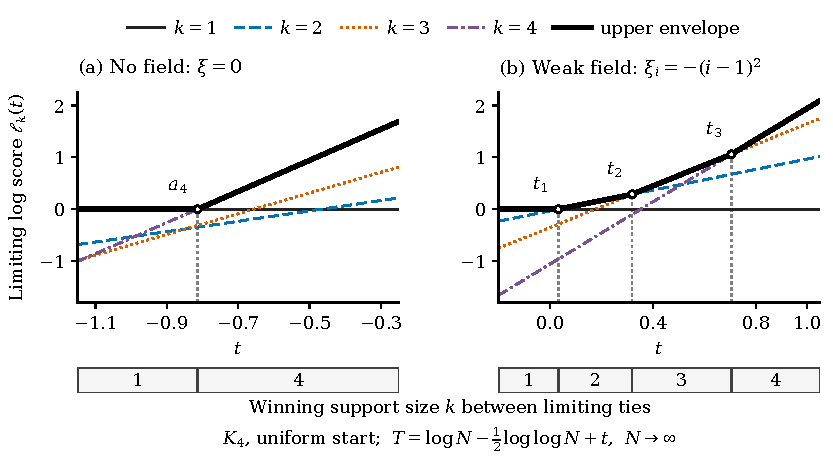
\includegraphics[width=0.52\textwidth]{fig_complete_envelope}
\caption{Support selection on the complete graph with four states, unit rates
and uniform start, in the window $T=\log N-\frac12\log\log N+t$.
Thin lines are limiting log face maxima relative to a vertex,
and the bold curve is their upper envelope. The winner jumps from one state
to all four at $t=a_4$. The scores are derived in Section~\ref{sec:complete},
and the marked tie concerns the limit, not a finite-$N$ equality}
\label{fig:complete-envelope}
\end{figure}
\else
\subsection{The complete graph and the layer near a vertex}\label{sec:intro-complete}

On the complete graph with the uniform start, $Q=J-dI$ with $J$ the all-ones matrix, every face
ties at first order and the constants decide. Sections~7 and~8 of the arXiv version of this
paper~\cite{arxivC1} treat this case, partly by the general theory and partly by exact arguments
of our preprint~\cite{paperB}, which this paper supersedes. A face of $k\ge2$ states crosses a
vertex exactly once, at a value $T_{N,k}$ with
\[
 T_{N,k}+\tfrac12\log T_{N,k}=\log N+a_k+O\Bigl(\frac1{\log N}\Bigr),\qquad
 a_k=\frac12\log(4\pi)-\frac{k+\frac12}{k-1}\log k .
\]
For $T\le N/d$ the most likely compositions
with a given support are those whose positive coordinates differ by at most $1$. Since
$a_2>a_3>\dots>a_d$, for large $N$ and $T$ up to a fixed multiple of $\log N$ the mode changes exactly once, from
the vertices straight to the compositions with $d$ positive coordinates. Near a vertex, for one
large count $b$ and small counts $a_1,\dots,a_\ell$, the crossing with a vertex lies at the odds
$\sqrt{y_a/b}\,(1+O(\sqrt{(|a|+1)/b}))$ of a switch, where $y_a$ is the positive root of
$\mathcal B(y)=1$ for an explicit polynomial $\mathcal B$ built from Laguerre polynomials. Then
$T$ is of order $\sqrt N$, and the lattice kernel of Theorem~\ref{thm:layer-counts} cannot be replaced by the Bessel kernel. This version leaves out
those two sections and keeps the numbers of the arXiv version, so Section~\ref{sec:boundary-layer}
is followed by Section~\ref{sec:verify}.
\fi

\subsection{Related work}\label{sec:related}

The exact law of the count vector goes back to Whittle~\cite{whittle1955},
Dawson and Good~\cite{dawsongood1957}, Goodman~\cite{goodman1958} and
Good~\cite{good1961}. For two states it is the Markov binomial law, whose exact form Gabriel~\cite{gabriel1959} gave. Dobrushin~\cite{dobrushin1953} found the limit laws of the number of visits of a two-state chain whose switch probabilities
scale with the length, and for switch probabilities of order $1/N$ the limit is
not Gaussian. This is the case $d=2$ of our regime. \v{C}ekanavi\v{c}ius and
Vellaisamy~\cite{cv2010} give compound Poisson approximations to the Markov
binomial law and cite the work on it since Dobrushin. Stadje~\cite{stadje1999}
finds the joint laws of the numbers of visits and their limits when one state
becomes nearly absorbing, with the transition probabilities out of it of order
$1/N$. Here every row of the transition matrix degenerates at the same rate.
Good proposed a saddle-point analysis of his formula (10) and did not carry it
out~\cite[pp.~42--43]{good1961}, and Theorem~\ref{thm:local}(a) is that analysis,
uniform in $T$ and with its constant. Part (b) does the same for his discrete
formula (3), uniformly in $T/N\le h_*$. Polettini~\cite{polettini2015} and
Carugno, Vivo and Coghi~\cite{cvc2022} derive the exact law from the BEST and
matrix-tree theorems.

For a fixed chain the occupation counts form a Markov additive process, and its
large deviations are classical. Miller~\cite{miller1961} proves a local large deviation theorem from the Perron root of the transform matrix, Ney and Nummelin~\cite{nn1987a,nn1987b} obtain the rates from its convergence parameter on general state spaces,
Kontoyiannis and Meyn~\cite[Theorem~6.3]{km2003} give exact large deviation
asymptotics for a real functional, and Herv\'e and Ledoux~\cite{herveledoux2013}
prove a local limit theorem for densities of the additive component. These
results concern a fixed transition matrix, and their constants depend on it. For
instance, Theorems~6.3 and~6.5 of~\cite{km2003} give the exact asymptotics of
$\Prob\{S_n\ge nc\}$ as $n\to\infty$, where $S_n$ is the partial sum of a real
functional of one geometrically ergodic chain, in the non-lattice and the lattice case, with no rate in $n$ and no
uniformity over kernels. Here the matrix $I+hQ$ tends to the identity and its
spectral gap $T/N$ tends to $0$, so these results give no bound uniform in $N$.
Theorem~\ref{thm:local}(b) is an exact local large deviation estimate for the whole
count vector of the chain killed on leaving $F$, with an explicit constant, and the
new point is that it is uniform as $I+hQ\to I$. At $h=0$ it joins
Theorem~\ref{thm:local}(a), the same estimate for the occupation times of the
continuous-time chain. We found no statement in these sources that covers either,
and none that is uniform as the chain degenerates.

In continuous time, Brydges, van der Hofstad and K\"onig~\cite{bhk2007} give an
explicit formula for the joint density of the local times on the event that the
range is a given set, and use it for large deviation upper bounds beyond the
exponential scale. On the event that the range up to time $T$ is $F$,
Lemma~\ref{lem:continuum} gives this density, mixed over the start and written
as Good's run expansion, and Theorem~\ref{thm:local}(a) gives its exact asymptotics
on compact subsets of the open face. Huang, Kious, Sidoravicius and
Tarr\`es~\cite{hkst2018} write the joint density of the local times, the last
exit tree and the cycling numbers of a chain with symmetric rates as a product
of Bessel functions, one for each edge. Pedler's occupation-time density for
two-state chains~\cite{pedler1971} and the Bessel forms of Kovchegov, Meredith
and Nir~\cite{kmn2010} for the occupation time of one state are exact formulas
for a fixed chain too. In the boundary layer the Bessel kernel arises
differently. It is the large-$T$ form of the contribution of the visits to one
state, after the facet is integrated out by a local law, and without
$\pi^{\rm in}=\pi^{\rm out}$ it can fail beyond $x$ of order $T^{1/3}$.

The rate inside a face is the Donsker and Varadhan functional of the killed
chain~\cite{dv1975,dupuisliu2015,chendeng2013}. Guillin, Nectoux and
Wu~\cite{gnw2024} prove a large deviation principle for the occupation measure
of a process conditioned to stay in a set. The quasi-ergodic law goes back to
Darroch and Seneta~\cite{darrochseneta1965,darrochseneta1967}, and Collet,
Mart\'inez and San Mart\'in~\cite{cmsm2013} is the standard reference. Dietz and
Sethuraman~\cite{dietz2007,dietz2005}, Bouguet and
Cloez~\cite{bouguetcloez2018} and Bena\"im, Bravo and Faure~\cite{bbf2026}
study chains whose switching decays along the trajectory, while here the rate is
fixed during each path and changes with $N$. Bertini, Gabrielli and
Landim~\cite{bgl2024}, Landim~\cite{landim2023} and Kim and Landim~\cite{kl2024}
expand the rate functions of a fixed chain in a parameter, the last for the
joint rate of the empirical measure and the flow~\cite{bfg2014,bfg2015}. Here
the functional enters through its restriction to each face, and faces of
different dimension compete.

The two-state walk is treated at every $N$ in~\cite{paperA}. Our
preprint~\cite{paperB} on the complete graph is \ifarxivbuild the first version
of this arXiv entry, and this version replaces it\else superseded by this
paper\fi. Table~\ref{tab:overlap} lists the results of \Bversion\ that we
reprove, where, which part, and how.\ifarxivbuild\else\ Sections~7 and~8 of the arXiv version of
this paper~\cite{arxivC1} reprove in addition Proposition~2.2, Theorems~3.1, 3.2 and~3.8,
Lemma~3.5, Proposition~3.6, Corollary~3.9, Example~3.10, Lemma~6.1 and Theorem~6.4
of~\cite{paperB}, and Table~1 there says how.\fi{} The other results of~\cite{paperB} are not
reproved here, namely Proposition~2.1, Proposition~3.7, Sections~4 and~5 on a
start and a field, Theorem~6.2, Remark~6.3 and Appendix~C. A companion
paper\ifarxivbuild~\cite{paperC2}\else, in preparation,\fi{} asks what the Donsker and Varadhan functional and the modal
supports determine about the generator.

\begin{table}[t]
\centering
\small
\caption{Results of \Bversion~\cite{paperB} reproved here. ``General'' means
that the proof is a case of the general theory of Sections~\ref{sec:model}
to~\ref{sec:secondorder}\ifarxivbuild, and ``as in~\cite{paperB}'' that it is the exact
argument of the preprint\fi}
\label{tab:overlap}
\begin{tabular}{@{}p{0.17\textwidth}p{0.25\textwidth}p{0.27\textwidth}p{0.2\textwidth}@{}}
\toprule
Item of~\cite{paperB} & Result here & Part covered & Method\\
\midrule
\ifarxivbuild
Prop.~2.2 & Lemma~\ref{lem:refresh}, \eqref{eq:runform}, \eqref{eq:SnVN} & all & as in~\cite{paperB}, with the run form from Lemma~\ref{lem:runs}\\
Thm.~3.1 & Cor.~\ref{cor:paperB}, Thm.~\ref{thm:simplex-crossing}(ii), (iv) & (ii) to (iv), and (i) without the term $-(k-1)/(8T)$ & general, and (iv) as in~\cite{paperB}\\
Thm.~3.2 & Thm.~\ref{thm:simplex-crossing}(i), (iii) & all but the term $1/(8T_{N,k})$ and the third-order expansion & (i) as in~\cite{paperB}, and (iii) general\\
Thm.~3.3 & Thm.~\ref{thm:stratified}, Ex.~\ref{ex:complete-face} & the local law (7), not the root (8) & general\\
Lemmas~3.4 and~3.5, Prop.~3.6 & Lemma~\ref{lem:weighted-cayley}, Prop.~\ref{prop:constant}(b), Ex.~\ref{ex:complete-face} & all but Prop.~3.6(5) & general, and Lemma~3.5 as in~\cite{paperB}\\
Thm.~3.8 & Thm.~\ref{thm:simplex-balance} & all & as in~\cite{paperB}\\
Cor.~3.9 & Cor.~\ref{cor:simplex-modes} & all & as in~\cite{paperB}, with Thm.~\ref{thm:simplex-crossing}(ii)\\
Ex.~3.10 & Rem.~\ref{rem:simplex-edge-mode} & all & as in~\cite{paperB}\\
Lemma~6.1 & Lemma~\ref{lem:uniform-laguerre-bessel} & all & as in~\cite{paperB}\\
Thm.~6.4 & Thm.~\ref{thm:vertex-uniform-root} & all & as in~\cite{paperB}\\
\else
Thm.~3.3 & Thm.~\ref{thm:stratified} & the local law (7) up to the closed form of its constant, not the root (8) & general\\
Lemma~3.4 & Prop.~\ref{prop:constant}(b) & all & general\\
\fi
\bottomrule
\end{tabular}
\end{table}

\emph{Organization.} Section~\ref{sec:model} sets up the exact law and
Section~\ref{sec:dv} the killed functional, in continuous and in discrete time. Section~\ref{sec:firstorder} proves
first-order face selection and gives the face maxima of reducible faces. It uses the local law and the face maxima of
Section~\ref{sec:secondorder}, whose proofs do not use
Section~\ref{sec:firstorder}. Section~\ref{sec:boundary-layer} treats the
boundary layer, \ifarxivbuild Sections~\ref{sec:complete} and~\ref{sec:vertex} the complete
graph, \fi and Section~\ref{sec:verify} the checks and the open questions.\ifarxivbuild\else\ The
arXiv version of this paper~\cite{arxivC1} has in addition Sections~7 and~8, on the complete graph
and near a vertex, with Appendices~C and~D. Its other sections and statements have the same numbers
as here.\fi

\section{Setting, notation and the exact law}\label{sec:model}

\subsection{Setting and notation}\label{sec:notation}

\emph{The chain.} Fix $d\ge2$ and a generator $Q$ on $[d]=\{1,\dots,d\}$. Its
rates are $q_{ij}\ge0$ for $i\ne j$, the exit rates are $q_i=\sum_{j\ne i}q_{ij}$,
$Q_{ii}=-q_i$, and $q_{\max}=\max_iq_i$. We also write $q$ for the vector
$(q_i)$. (The scalar $q=1-p$ of the two-state
walk appears only where we recall~\cite{paperA}, and the scalar $q$ of
Proposition~\ref{prop:pair} is a common exit rate.) The start
$\mu$ is a probability law on $[d]$, and $\mu(F)=\sum_{i\in F}\mu_i$. We write
$V=[d]$ for the face of all states. For $N\ge2$
and $T>0$ put
\[
 h=\frac TN,\qquad L=\log N,\qquad \tau=\frac TL .
\]
The chain $X_1,\dots,X_N$ has $X_1\sim\mu$ and transition matrix $I+hQ$. So at
each step it jumps from $i$ to $j$ with probability $hq_{ij}$, and $N$ steps
look like the continuous-time chain with generator $Q$ run for time $T$. We
assume $hq_{\max}\le\frac12$ unless we say otherwise. The \emph{composition} is
the vector of visit counts $n=(n_1,\dots,n_d)$, with
$n_i=\#\{t\le N:X_t=i\}$, so that $n_1+\dots+n_d=N$. We write $P_N(n)$ for the
probability that the chain has composition $n$, $\supp n=\{i:n_i>0\}$ for its
support, and $\alpha=n/N$ for the visit fractions.

\emph{Faces.} A face is a nonempty set $F\subseteq[d]$, of size
$k=k_F=\lvert F\rvert$. Let $\Delta_F$ be the set of probability vectors on
$[d]$ that vanish off $F$, and $\Delta_F^\circ$ the set of those that are
positive on $F$. We number the states of $F$ as $1,\dots,k$ and use the
coordinates $(\alpha_2,\dots,\alpha_k)$ on $\Delta_F$ and $(t_2,\dots,t_k)$ on
$\{t\in\R^F:t_1+\dots+t_k=T\}$. We write $x\cdot y=\langle x,y\rangle
=\sum_{i\in F}x_iy_i$ and $x\circ y=(x_iy_i)_{i\in F}$. Let
$A_F=(q_{ij})_{i,j\in F}$ with zero diagonal, and $Q_F=A_F-\operatorname{diag}
(q_i)_{i\in F}$. Since $q_i$ includes the rates of leaving $F$, $Q_F$ generates
the chain killed when it leaves $F$. The switching graph $G_F$ has an edge
$i\to j$ whenever $i,j\in F$, $i\ne j$ and $q_{ij}>0$.

\emph{Perron roots.} A square matrix $B$ is Metzler if its off-diagonal entries
are nonnegative, and then its Perron root $\varrho(B)$ is its largest real
eigenvalue.
If $B$ is irreducible, $\varrho(B)$ is simple and has positive left and right
eigenvectors~\cite{bermanplemmons1994}.

\begin{definition}[faces]\label{def:faces}
Let $F$ be a face. We call $F$ \emph{irreducible} if $G_F$ is strongly connected.
In particular every singleton is irreducible. We call $F$ \emph{admissible} if for some
$N$ some path $x_1\cdots x_N$ of positive probability has support exactly $F$
(for $0<hq_{\max}<1$ this does not depend on $h$).
We say that $F$ satisfies \textup{(H)} if $F$ is irreducible and $\mu(F)>0$.
The \emph{exit rate} of $F$ is $\lambda_F=-\varrho(Q_F)$, so
$\lambda_{\{i\}}=q_i$. If $F$ is irreducible, $r_F$ and $l_F$ are right and left
eigenvectors of $Q_F$ for $-\lambda_F$ with positive entries and
$\langle l_F,r_F\rangle=1$, and $\alpha^*_F=l_F\circ r_F$ is the
\emph{quasi-ergodic law} of $F$~\cite{darrochseneta1965,darrochseneta1967}. The
\emph{face maximum} is $M_F=\max\{P_N(n):\supp n=F\}$, with $\max\emptyset=0$.
\end{definition}

We call $\lambda_F$ the exit rate for the following reason. If $F$ is
irreducible, then $e^{TQ_F}r_F=e^{-T\lambda_F}r_F$ and $r_F$ is positive. So
the chance that the continuous-time chain started at a state of $F$ stays in
$F$ up to time $T$, which is a row sum of $e^{TQ_F}$, lies between
$e^{-T\lambda_F}\min r_F/\max r_F$ and $e^{-T\lambda_F}\max r_F/\min r_F$. If
$F$ is reducible, we order the strongly connected components $C_1,\dots,C_r$ of
$G_F$ so that every edge between components goes forward. Then $Q_F$ is block
triangular with diagonal blocks $Q_{C_j}$, and
$\lambda_F=\min_j\lambda_{C_j}$. In all cases $0\le\lambda_F\le\min_{i\in
F}q_i$, since the rows of $Q_F$ have sums at most $0$ and a Perron root is at
least every diagonal entry. For a face $F$ satisfying (H), the quasi-ergodic law
$\alpha^*_F$ is the long-run law of the visit fractions of the chain conditioned
to stay in $F$, and the best composition on $F$ sits near $N\alpha^*_F$
(Theorem~\ref{thm:facemax}).

\emph{The two-state walk.} The persistent random walk on $\Z$ makes its first
step left or right with probability $\frac12$, and each later step repeats the
previous one with probability $p$ and switches with probability $q=1-p$. Its
directions form the chain of Example~\ref{ex:models}(i). As on a Galton board,
\cite{paperA} calls a composition a \emph{bin}. For two states we identify a composition
with its number of right steps. For $a,b\ge1$ let
$S_{a,b}(u)=\sum_wu^{s(w)}$, the sum
over the words $w$ with $a$ right steps and $b$ left steps, where $s(w)$ is the
number of switches of $w$. Each such word has probability
$\frac12p^{N-1}(q/p)^{s(w)}$ for the walk with $N=a+b$ steps. So
$S_{a,b}(q/p)$ is the probability of composition $a$ divided by the probability
$\frac12p^{N-1}$ of an endpoint. For $N\ge2$ let
$S_N=S_{\lfloor N/2\rfloor,\lceil N/2\rceil}$, which belongs to a middle composition.
It is a nonzero polynomial with nonnegative coefficients
and no constant term, so $S_N(u)=1$ has exactly one positive root $u_N$, and
$p_N=1/(1+u_N)$ is the crossing of the middle and the endpoints. Put
$z_N=N(1-p_N)$ and $c_0=\frac12\log(\pi/8)$. By~\cite{paperA}, $z_N$ satisfies
the crossing equation $z_N+\frac12\log z_N=L+c_0+1/(8z_N)+O(1/L^2)$. We recall this
expansion only for comparison with Corollary~\ref{cor:paperA}.

\emph{Conventions.} Unless we say otherwise, $Q$, $\mu$ and the faces under
discussion are fixed, and every constant, every implied constant in $O(\cdot)$
and every threshold $N_0$ depends only on them and on the compact set
$\mathcal K$ when one appears. A bound that holds ``uniformly for $1\le T\le
N^{1/3}$'' holds for all $N\ge N_0$ and all $T$ in that range with one implied
constant. Subscripts as in $O_{\mathcal K}$ stress a dependence.

\subsection{Admissible faces}

\begin{lemma}[admissible faces]\label{lem:admissible}
Let $F$ be a face and $C_1,\dots,C_r$ the strongly connected components of
$G_F$. \textup{(a)} $F$ is admissible if and only if the components can be
numbered so that $\mu(C_1)>0$ and, for each $j<r$, $q_{xy}>0$ for some $x\in
C_j$ and $y\in C_{j+1}$. \textup{(b)} An irreducible face is admissible if and
only if $\mu(F)>0$. So \textup{(H)} holds exactly for the irreducible admissible
faces. \textup{(c)} If $Q$ has symmetric support, that is $q_{ij}>0$ exactly
when $q_{ji}>0$, then every admissible face is irreducible.
\end{lemma}

\begin{proof}
We translate paths into walks in $G_F$. Take a path of positive probability
with support $F$ and list the states of its maximal runs. This list is a walk
in $G_F$ that starts at a state of $\supp\mu$ and visits every state of $F$.
Conversely, every such walk $v_1,\dots,v_J$ is the list of runs of a path of
positive probability with support $F$, as soon as $N\ge J$. (The path follows the walk and then stays in its last state, and a stay
has positive probability.) So $F$ is admissible exactly when $G_F$ has a walk
that starts in $\supp\mu$ and visits every state of $F$.

(a) Suppose that there is such a walk. Once it has left a component $C$ for a
state $y\notin C$, it cannot come back to $C$. (If it did, $y$ could be reached
from $C$ and $C$ from $y$, so $y$ would belong to $C$.) Hence the walk visits
each component in one block of consecutive times, and it passes from one block
to the next along a single edge. We number the components in the order of these
blocks. The walk starts in $C_1$, so $\mu(C_1)>0$, and the edge from block $j$
to block $j+1$ is an edge $x\to y$ with $x\in C_j$ and $y\in C_{j+1}$. This is
the condition in (a).

Conversely, suppose that the components are numbered as in (a), with edges
$x_j\to y_{j+1}$ from $C_j$ to $C_{j+1}$ for $j<r$. Take $y_1\in C_1$ with
$\mu_{y_1}>0$ and any $x_r\in C_r$. Since $C_j$ is strongly connected, there is
a walk inside $C_j$ from $y_j$ to $x_j$ that visits every state of $C_j$. We
join these $r$ walks by the edges $x_j\to y_{j+1}$. The result is a walk that
starts in $\supp\mu$ and visits every state of $F$.

(b) This is (a) with $r=1$.

(c) If $Q$ has symmetric support, an edge from one component to another would
come with an edge back, and the two components would be the same. So no edge
joins two components, and the condition in (a) forces $r=1$.
\end{proof}

So $M_F>0$ for large $N$ if $F$ is admissible, and $M_F=0$ otherwise.

\subsection{The exact law}

For $m\in\Z_{\ge1}^F$ put $M=\sum_{i\in F}m_i$ and
$W(m)=\sum_c\mu_{c_1}\prod_{j<M}q_{c_jc_{j+1}}$, the sum over the words
$c=c_1\cdots c_M$ in $F$ with $c_j\ne c_{j+1}$ in which each $i\in F$ occurs
$m_i$ times. Such a word lists the states of the runs of a path, and $m_i$ is
the number of runs in state $i$.

\begin{lemma}[run expansion]\label{lem:runs}
Let $hq_{\max}\le1$ and let $n$ have support $F$. Then, with
$\binom{n_i-1}{m_i-1}=0$ for $m_i>n_i$ and $0^0=1$,
\[
P_N(n)=\sum_{m\in\Z_{\ge1}^F}W(m)\,h^{M-1}\prod_{i\in F}\binom{n_i-1}{m_i-1}
(1-hq_i)^{n_i-m_i}.
\]
\end{lemma}

This is Good's coefficient identity~\cite[(3)]{good1961}, with the exponents
$n_i-1$, for a chain of $N$ letters with any initial law, here for the chain
killed on leaving $F$. Grouping by runs is our way of writing it, and the proof
is short.

\begin{proof}
The states $c_1\cdots c_M$ of the maximal runs of a path with composition $n$
form a word as in $W(m)$. The path starts at $c_1$, of probability
$\mu_{c_1}$, it has $M-1$ switches, of probabilities $hq_{c_jc_{j+1}}$, and
$n_i-m_i$ stays in state $i$, of probability $1-hq_i$ each. The number of paths
with the word $c$ and composition $n$ is $\prod_i\binom{n_i-1}{m_i-1}$, the number
of ways to write each $n_i$ as an ordered sum of $m_i$ positive run lengths.
Summing over the words $c$ with given $m$ gives $W(m)$, and summing over $m$ gives
the claim.
\end{proof}

Lemma~\ref{lem:runs} is checked in Lean (Section~\ref{sec:verify}). For
$F=\{i\}$ the only path is $i^N$, so uniformly for $1\le T\le N^{1/2}$
\begin{equation}\label{eq:vertexmax}
M_{\{i\}}=\mu_i(1-hq_i)^{N-1}=\mu_ie^{-q_iT}\bigl(1+O(T^2/N)\bigr).
\end{equation}
For $t\in(0,\infty)^F$ let $H(t)=\sum_mW(m)\prod_{i\in F}t_i^{m_i-1}/(m_i-1)!$,
which is finite since $W(m)\le k^Mq_{\max}^{M-1}$. In the continuum limit the
binomial coefficients of Lemma~\ref{lem:runs} become the powers
$t_i^{m_i-1}/(m_i-1)!$, and Lemma~\ref{lem:discrete} below shows that the discrete
law is close to the following density.

\begin{lemma}[the continuum density]\label{lem:continuum}
Let $(Y_s)_{s\ge0}$ be the continuous-time chain with generator $Q$ and
$Y_0\sim\mu$, let $\mathcal O_i=\int_0^T\mathbf 1\{Y_s=i\}\,ds$, and let $E_F$
be the event that $Y$ stays in $F$ during $[0,T]$ and visits every state of $F$.
Then $\Prob(E_F,\ \mathcal O\in\cdot\,)$ has the density
$e^{-\langle q,t\rangle}H(t)$ in $(t_2,\dots,t_k)$ on
$\{t\in(0,\infty)^F:\sum_it_i=T\}$, and $\Prob(E_F,\ \mathcal O/T\in\cdot\,)$
has the density
\[
f_T(\alpha)=T^{k-1}e^{-T\langle q,\alpha\rangle}H(T\alpha)
\]
in $(\alpha_2,\dots,\alpha_k)$. For $n$ with support $F$ and $t=hn$,
$N^{-(k-1)}f_T(n/N)=h^{k-1}e^{-\langle q,t\rangle}H(t)$. For $F=\{i\}$,
$f_T=\Prob(E_F)=\mu_ie^{-q_iT}$.
\end{lemma}

The density is Good's formula~\cite[(10)]{good1961}. What we add is the killing,
that is, the subprobability with the full exit rates $q_i$ on the diagonal, and
the exponents $m_i-1$, which the proof checks.

\begin{proof}
Up to a null set, $E_F$ is the disjoint union of the events $E_c$ that $Y$
visits exactly $c_1,\dots,c_M$ in this order during $[0,T]$, over the words $c$
in the sums $W(m)$. Fix $c$, and let $s_j$ be the time that $Y$ spends in its
$j$-th run, so that $s_1+\dots+s_M=T$. For $j<M$ the run has the density
$q_{c_j}e^{-q_{c_j}s_j}$ and ends with a jump to $c_{j+1}$ of probability
$q_{c_jc_{j+1}}/q_{c_j}$, and the last run survives with probability
$e^{-q_{c_M}s_M}$. So on $\{s_j>0\ \forall j\}$ the event $E_c$ has the density
$\mu_{c_1}\prod_{j<M}q_{c_jc_{j+1}}\,e^{-\langle q,\mathcal O\rangle}$ in
$(s_1,\dots,s_{M-1})$, where $\mathcal O_i$ is the sum of the $s_j$ with $c_j=i$.
For each $i\ne c_M$ we replace the last holding time in state $i$ by
$\mathcal O_i$, a triangular change of variables with unit diagonal. With
$\mathcal O=t$ fixed, the $m_i-1$ other holding times in state $i$ are positive
with sum less than $t_i$, so they range over a simplex of volume
$t_i^{m_i-1}/(m_i-1)!$. Integrating them out gives the density
$\mu_{c_1}\prod_{j<M}q_{c_jc_{j+1}}\,e^{-\langle q,t\rangle}\prod_it_i^{m_i-1}/(m_i-1)!$
in the coordinates $t_i$ with $i\ne c_M$, and any $k-1$ of the coordinates give
the same Lebesgue measure on $\{\sum_it_i=T\}$. Summing over $c$ and $m$ gives
$e^{-\langle q,t\rangle}H(t)$, and $t=T\alpha$ has Jacobian $T^{k-1}$. For
$F=\{i\}$ the event $E_F$ says that $Y$ starts at $i$ and does not jump before
time $T$.
\end{proof}

\begin{example}[two models]\label{ex:models}
(i) For $d=2$, $q_{12}=q_{21}=1$ and uniform $\mu$ the chain is the persistent
walk, with $p=1-h$. So $T=N(1-p)$, the faces
$\{1\}$ and $\{2\}$ are the endpoints, and Lemma~\ref{lem:runs} is the run count
for two states. (ii) For $Q=J-dI$, with $J$ the all-ones matrix, the chain
switches to each other state with probability $h$ and keeps its state with
probability $p=1-(d-1)h$. With uniform $\mu$ it is the model of~\cite{paperB},
whose switch probability $r$ is our $h$. A word $x_1\cdots x_N$ then has
probability $\frac1dh^{N-1}(p/h)^{\#\{s<N:\,x_s=x_{s+1}\}}$, so the path law is the
one-dimensional $d$-state Potts chain with free boundaries. Here $q_i=d-1$ for
every $i$, so Lemma~\ref{lem:runs} reads
\begin{equation}\label{eq:runform}
 P_N(n)=p^{N-1}\sum_{a\in F}\mu_aS^{(a)}_n(u),\qquad u=\frac hp,
\end{equation}
for $p>0$ and $\supp n=F$, where $S^{(a)}_n(u)$ is the sum of $u^j$ over the words with
the counts $n$ that start with $a$ and have $j$ switches. Indeed such a word has
probability $\mu_ap^{N-1-j}h^j=\mu_ap^{N-1}u^j$. In both models $Q$ has symmetric
support and $\mu$ full support, so all admissible faces satisfy \textup{(H)} by
Lemma~\ref{lem:admissible}.
\end{example}
Figure~\ref{fig:simplex} shows exact support competition for the three-state path.
There $\lambda_F$ is $1$ for an end, $(3-\sqrt5)/2$ for a pair of neighbors and
$0$ for all three states, so to first order the mode moves at
$\tau=(1+\sqrt5)/2$ and at $\tau=(3+\sqrt5)/2$, that is, at $T=7.3$ and
$T=11.8$ for $N=90$. At $N=90$ it moves near $T=4.9$ and $T=8.5$. Corrections of
this size are the subject of Section~\ref{sec:secondorder}.

\begin{figure}[t]
\centering
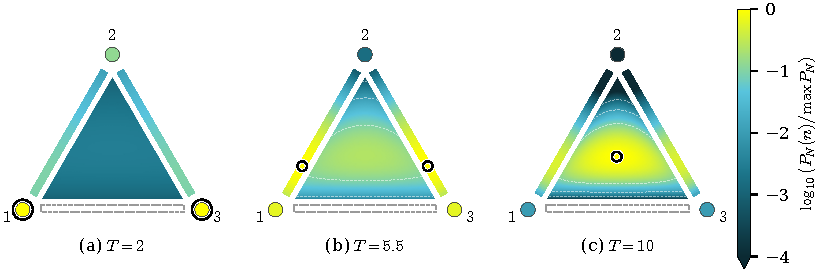
\includegraphics[width=\textwidth]{fig_simplex}
\caption{The exact law of the composition for the path $1-2-3$ (rate $1$ on
each edge, uniform start, $N=90$) on the simplex of visit fractions, with the
faces drawn apart. The triangle holds the compositions with three states, each
band those with two, and each disk a vertex. The color is the probability
relative to the mode, the thin lines are spaced by a factor of ten, and the
rings mark the modes. The mode is (a) at an end of the path, (b) on a pair of
neighbors and (c) inside. The dashed band $\{1,3\}$ has probability zero}
\label{fig:simplex}
\end{figure}

\section{The killed functional}\label{sec:dv}

Every rate in this paper is the restriction of one functional, the Donsker and
Varadhan functional of the chain.

\subsection{The restriction identity}\label{sec:restriction}

For a probability vector $\alpha$ on $[d]$ let
\begin{equation}\label{eq:JV}
 J_V(\alpha)=\sup_{u\in(0,\infty)^d}\sum_{i\in[d]}\alpha_i\Bigl(-\frac{(Qu)_i}{u_i}\Bigr)
 =\sup_{u\in(0,\infty)^d}\sum_{i\in[d]}\alpha_i\Bigl(q_i-\sum_{j\ne i}q_{ij}\frac{u_j}{u_i}\Bigr),
\end{equation}
the Donsker and Varadhan rate of the empirical measure of the continuous-time
chain with generator $Q$~\cite{dv1975}. For a face $F$ and $\alpha\in\Delta_F$ let
\[
 J_F(\alpha)=\sup_{u\in(0,\infty)^F}\sum_{i\in F}\alpha_i\Bigl(-\frac{(Q_Fu)_i}{u_i}\Bigr)
 =\sup_{u\in(0,\infty)^F}\sum_{i\in F}\alpha_i\Bigl(q_i-\sum_{j\in F\setminus\{i\}}q_{ij}\frac{u_j}{u_i}\Bigr),
\]
the same functional for the chain killed on leaving $F$. Let $q_i^{\rm out}(F)=\sum_{j\notin F}q_{ij}$. Taking $u=\ones$
gives $J_F(\alpha)\ge\sum_i\alpha_iq_i^{\rm out}(F)$, and dropping the terms
with $q_{ij}$ gives $J_F(\alpha)\le\sum_i\alpha_iq_i$.

\begin{proposition}[the restriction identity]\label{prop:restriction}
For every face $F$ and every $\alpha\in\Delta_F$, $J_F(\alpha)=J_V(\alpha)$. Hence
$J_F=J_{F'}$ on $\Delta_{F'}$ for every nonempty $F'\subseteq F$.
\end{proposition}

\begin{proof}
Fix $\alpha\in\Delta_F$ and $u\in(0,\infty)^d$. The terms of~\eqref{eq:JV} with
$i\notin F$ vanish, since $\alpha_i=0$ there. For $i\in F$ the terms with
$j\notin F$ are nonnegative and are subtracted, so
\[
 \sum_{i\in F}\alpha_i\Bigl(q_i-\sum_{j\ne i}q_{ij}\frac{u_j}{u_i}\Bigr)
 \le\sum_{i\in F}\alpha_i\Bigl(q_i-\sum_{j\in F\setminus\{i\}}q_{ij}\frac{u_j}{u_i}\Bigr)
 \le J_F(\alpha).
\]
So $J_V(\alpha)\le J_F(\alpha)$. Conversely, let $w\in(0,\infty)^F$ and let $u$
equal $w$ on $F$ and $\varepsilon$ off $F$. The terms with $j\notin F$ are then
$-q_{ij}\varepsilon/w_i$, which tend to zero as $\varepsilon\downarrow0$, and
the supremum over $w$ gives $J_V(\alpha)\ge J_F(\alpha)$. The second claim is the
first for $F$ and for $F'$.
\end{proof}

So the cost of a point of $\Delta_F$ does not depend on the face in which we
read it.

\subsection{The variational formula}\label{sec:spectral-geometry}

For a face $F$ and a field $v\in\R^F$ let
\begin{equation}\label{eq:lambdaFv}
 \lambda_F(v)=-\varrho\bigl(Q_F+\operatorname{diag}v\bigr),
\end{equation}
so that $\lambda_F(0)=\lambda_F$. If $F$ is irreducible, let $r$ and $l$ be
positive right and left Perron vectors of $Q_F+\operatorname{diag}v$ with
$l\cdot r=1$, and put $\alpha^*_F(v)=l\circ r$, so that $\alpha^*_F(0)=\alpha^*_F$.
Since $\sum_i\alpha_iv_i=v\cdot\alpha$,
\begin{equation}\label{eq:Jfield}
 J_F(\alpha)-v\cdot\alpha=\sup_{u\in(0,\infty)^F}\sum_{i\in F}\alpha_i
 \Bigl(-\frac{((Q_F+\operatorname{diag}v)u)_i}{u_i}\Bigr).
\end{equation}
So a field replaces the diagonal $q_i$ by $q_i-v_i$ and changes nothing else.

\begin{lemma}[monotonicity in the face]\label{lem:face-monotone}
If $F\subsetneq G$ are faces and $Q_G$ is irreducible, then
$\lambda_G(v_G)<\lambda_F(v_F)$ for every field $v\in\R^G$. Now let $Q$ be
irreducible. Then $\lambda_V(v)<\lambda_F(v_F)$ for every proper face $F$, and
for every fixed $v\in\R^d$ there is $\gamma(v)>0$ with
$\lambda_F(v_F)\ge\lambda_V(v)+\gamma(v)$ for all proper $F$. So the score
$\Phi_{\tau,v}(F)=|F|-1+\tau\lambda_F(v_F)$ is least at $V$ for
$\tau>(d-1)/\gamma(v)$.
\end{lemma}

The last two claims need $Q$ irreducible. For $d=2$, $q_{12}=1$ and $q_{21}=0$
we have $\lambda_V=0=\lambda_{\{2\}}$.

\begin{proof}
Choose $c$ with $B=Q_G+\operatorname{diag}v_G+cI\ge0$. Its principal submatrix on
$F$ is $Q_F+\operatorname{diag}v_F+cI$, since the diagonal of a killed generator
keeps the full exit rates. Let $\widetilde B$ be this submatrix padded with zeros
to $G\times G$. Then $0\le\widetilde B\le B$, and $\widetilde B\ne B$ because the
irreducible matrix $B$ has a positive entry in a row of $F$ and a column off $F$.
So $\varrho(\widetilde B)<\varrho(B)$~\cite[Ch.~2]{bermanplemmons1994},
and $\varrho(\widetilde B)$ is the Perron root of the submatrix on $F$, since the
padding adds only the eigenvalue $0$. This holds whether or not $F$ is
irreducible, and subtracting $c$ gives the first claim. If $Q$ is irreducible,
the first claim with $G=V$ gives the second. For fixed $v$ there are
finitely many proper faces, so $\gamma(v)$, the least of the numbers
$\lambda_F(v_F)-\lambda_V(v)$, is positive. Finally
$\Phi_{\tau,v}(F)-\Phi_{\tau,v}(V)=|F|-d+\tau(\lambda_F(v_F)-\lambda_V(v))\ge-(d-1)+\tau\gamma(v)$.
\end{proof}

\begin{proposition}[the rate on a face]\label{prop:rate}
Let $F$ be irreducible with $k=\lvert F\rvert\ge2$, and let $v\in\R^F$.
\begin{enumerate}[(a)]
\item On $\Delta_F$, $J_F(\alpha)-v\cdot\alpha\ge\lambda_F(v)$, with equality exactly at
$\alpha=\alpha^*_F(v)$. In particular $J_F\ge\lambda_F$, with equality exactly at
$\alpha^*_F=l_F\circ r_F$.
\item The rate $J_F$ is convex on $\Delta_F$ and strictly convex on $\Delta_F^\circ$. For
$\alpha\in\Delta_F^\circ$ the supremum defining $J_F(\alpha)$ is attained at a
vector $u=r_\alpha$, which is unique up to a positive factor, and $\alpha$ is
the stationary law of the generator on $F$ with off-diagonal entries
$q_{ij}r_{\alpha,j}/r_{\alpha,i}$.
\item If there is $\nu\in(0,\infty)^F$ with $\nu_iq_{ij}=\nu_jq_{ji}$ for all
$i,j\in F$, then for every $\alpha\in\Delta_F$
\[
 J_F(\alpha)=\sum_{\{i,j\}\subseteq F,\ i\ne j}\bigl(\sqrt{\alpha_iq_{ij}}-\sqrt{\alpha_jq_{ji}}\bigr)^2
 +\sum_{i\in F}\alpha_iq_i^{\rm out}(F).
\]
\item For every nonempty face $F'\subsetneq F$ and every
$\alpha\in\Delta_{F'}$, $J_F(\alpha)-v\cdot\alpha=J_{F'}(\alpha)-v\cdot\alpha\ge\lambda_{F'}(v_{F'})>\lambda_F(v)$.
\end{enumerate}
\end{proposition}

For symmetric $Q_F$, $l_F=r_F$ and $\alpha^*_F$ is the entrywise square of the
Perron vector normalized in $\ell^2$. On a face that is not reversible the
formula in (c) is only an upper bound, by its proof.

\begin{proof}
Put $B=Q_F+\operatorname{diag}v$, an irreducible Metzler matrix with the switching
graph $G_F$ and $\lambda_F(v)=-\varrho(B)$.

\emph{Setup.} With $u=e^\psi$, \eqref{eq:Jfield} reads
$J_F(\alpha)-v\cdot\alpha=\sup_\psi\Psi_\alpha(\psi)$ with
\[
\Psi_\alpha(\psi)=\sum_i\alpha_i(q_i-v_i)-\sum_{i\ne j}\alpha_iq_{ij}e^{\psi_j-\psi_i},
\]
where $i,j$ run over $F$. It is concave in $\psi$, affine in $\alpha$, and
unchanged when a constant is added to $\psi$. Let $G^\psi$ be the conservative
generator on $F$ with off-diagonal entries $q_{ij}e^{\psi_j-\psi_i}$. It has the
graph $G_F$, so it has exactly one stationary law, and it does not involve $v$.
Since $\nabla_\psi\Psi_\alpha=-\alpha^\top G^\psi$ and a differentiable concave
function attains its maximum exactly at its critical points, $\psi$ attains the
supremum if and only if $\alpha$ is the stationary law of $G^\psi$. We call this
the criterion.

\emph{A lower bound on every face.} Let $F'$ be any face, irreducible or not, and
$B'=Q_{F'}+\operatorname{diag}v_{F'}$. We show
$J_{F'}(\alpha)-v\cdot\alpha\ge-\varrho(B')$ on $\Delta_{F'}$. Let
$s>\varrho(B')$ and write $B'=B_0-cI$ with $B_0\ge0$. Then $s+c>\varrho(B_0)$, so
$u=(sI-B')^{-1}\ones=\sum_{\ell\ge0}(s+c)^{-\ell-1}B_0^\ell\ones$ converges and is
positive. Since $(sI-B')u=\ones$, we get $-(B'u)_i/u_i=-s+1/u_i>-s$ at every
state, and letting $s\downarrow\varrho(B')$ gives the claim.

\emph{The value at $\alpha^*_F(v)$.} Take $\psi=\log r$ and $R=\operatorname{diag}r$.
Then $G^\psi=R^{-1}(B-\varrho(B)I)R$, since the off-diagonal entries agree and
$Br=\varrho(B)r$. So $(l\circ r)^\top G^\psi=l^\top(B-\varrho(B)I)R=0$, and by the
criterion $\psi$ attains the supremum at $\alpha^*_F(v)$. Every ratio
$-(Br)_i/r_i$ equals $\lambda_F(v)$, so the value is $\lambda_F(v)$.

(b) Convexity holds because $J_F$ is a supremum of affine functions. Let
$\alpha\in\Delta_F^\circ$ and take $v=0$.

\emph{The supremum is attained.} Normalize $\min_i\psi_i=0$ and put
$\bar\psi=\max_i\psi_i$. Let $a$ be the least positive rate $q_{ij}$ in $F$. A
shortest path in $G_F$ from a state where $\psi=0$ to a state where
$\psi=\bar\psi$ has at most $k-1$ edges, so one of its edges $i\to j$ has
$\psi_j-\psi_i\ge\bar\psi/(k-1)$. Keeping only this edge gives
$\Psi_\alpha(\psi)\le\sum_i\alpha_iq_i-a(\min_i\alpha_i)e^{\bar\psi/(k-1)}$, which
tends to $-\infty$ as $\bar\psi\to\infty$. So the continuous function
$\Psi_\alpha$ attains its supremum on a bounded set. Write $r_\alpha=e^\psi$ for a
maximizer. The last claim of (b) is the criterion.

\emph{The maximizer is unique up to a factor.} If $\psi$ and $\psi+\delta$ both
attain the supremum, $\Psi_\alpha$ is constant on the segment between them. There
it is a constant minus a sum of the convex functions
$\alpha_iq_{ij}e^{\psi_j-\psi_i+s(\delta_j-\delta_i)}$, so each of them is affine
in $s$, and $\delta_j=\delta_i$ on every edge of $G_F$. As $G_F$ is strongly
connected, $\delta$ is constant.

\emph{Strict convexity.} Let $\alpha^0\ne\alpha^1$ lie in $\Delta_F^\circ$, put
$\alpha^s=(1-s)\alpha^0+s\alpha^1$ with $0<s<1$, and let $\psi$ attain
$J_F(\alpha^s)$. Since $\Psi_\alpha(\psi)$ is affine in $\alpha$,
$J_F(\alpha^s)=(1-s)\Psi_{\alpha^0}(\psi)+s\Psi_{\alpha^1}(\psi)\le(1-s)J_F(\alpha^0)+sJ_F(\alpha^1)$.
Equality would make $\alpha^0$ and $\alpha^1$ both stationary for $G^\psi$ by the
criterion, which is impossible.

(d) The equality is Proposition~\ref{prop:restriction}. The lower bound on $F'$
gives $J_{F'}(\alpha)-v\cdot\alpha\ge\lambda_{F'}(v_{F'})$, and
Lemma~\ref{lem:face-monotone} with $G=F$ gives $\lambda_{F'}(v_{F'})>\lambda_F(v)$.

(a) The lower bound and the value at $\alpha^*_F(v)$ are proved above. Let
$\alpha\ne\alpha^*_F(v)$. If $\alpha$ lies on the boundary of $\Delta_F$, then (d)
with $F'=\supp\alpha$ gives $J_F(\alpha)-v\cdot\alpha>\lambda_F(v)$. If
$\alpha\in\Delta_F^\circ$ and equality held, strict convexity would give a value
below $\lambda_F(v)$ at $\frac12(\alpha+\alpha^*_F(v))$.

(c) Since $q_i=\sum_{j\in F\setminus\{i\}}q_{ij}+q_i^{\rm out}(F)$, the function
inside the supremum is $\sum_i\alpha_iq_i^{\rm out}(F)$ plus, for each pair
$\{i,j\}$, the term $\alpha_iq_{ij}(1-u_j/u_i)+\alpha_jq_{ji}(1-u_i/u_j)$. By the
AM--GM inequality this term is at most
$(\sqrt{\alpha_iq_{ij}}-\sqrt{\alpha_jq_{ji}})^2$, which gives the upper bound. For
$\alpha\in\Delta_F^\circ$ the vector $u_i=\sqrt{\alpha_i/\nu_i}$ gives
$\alpha_iq_{ij}u_j/u_i=\alpha_jq_{ji}u_i/u_j$ by $\nu_iq_{ij}=\nu_jq_{ji}$, so there is
equality for every pair at once. If some $\alpha_i$ vanish, take $u_i=\varepsilon$
for these $i$ and let $\varepsilon\to0$. A pair with $\alpha_i=0<\alpha_j$ then has
the term $\alpha_jq_{ji}(1-\varepsilon/u_j)\to\alpha_jq_{ji}$, which is its bound, and
a pair with $\alpha_i=\alpha_j=0$ has the term $0$.
\end{proof}

\begin{proposition}[the variational formula]\label{prop:variational}
Let $F$ be irreducible. For every $v\in\R^F$,
\[
 \lambda_F(v)=\min_{\alpha\in\Delta_F}\bigl(J_F(\alpha)-v\cdot\alpha\bigr),
\]
and the minimum is attained only at $\alpha^*_F(v)$. Equivalently, $-\lambda_F(v)$
is the Legendre transform of $J_F$ at $v$, and $J_F$ is the Legendre transform of
$v\mapsto-\lambda_F(v)$ on $\Delta_F^\circ$. The map $v\mapsto\lambda_F(v)$ is
concave and real-analytic, and $\lambda_F(v+c\ones)=\lambda_F(v)-c$. If $Q_F$ is
reversible with respect to $\nu$, let $S_F=D_{\sqrt\nu}(-Q_F)D_{\sqrt\nu}^{-1}$, where $D_x=\operatorname{diag}x$.
Then with $\psi_i=\sqrt{\alpha_i}$,
\[
 J_F(\alpha)-v\cdot\alpha=\sum_{i\in F}(q_i-v_i)\alpha_i-\sum_{i\ne j\in F}\sqrt{q_{ij}q_{ji}}\,\psi_i\psi_j
\]
is the Rayleigh quotient of the symmetric matrix $S_F-\operatorname{diag}v$ at the
unit vector $\psi$, and $\lambda_F(v)=\lambda_{\min}(S_F-\operatorname{diag}v)$.
\end{proposition}

The formula is the finite form of the Donsker and Varadhan formula for the
principal eigenvalue~\cite{dv1975}, close to the characterization of Collatz and
Wielandt~\cite[Ch.~2]{bermanplemmons1994}.

\begin{proof}
The formula and the unique minimizer are Proposition~\ref{prop:rate}(a). As a
minimum of affine functions of $v$, $\lambda_F(v)$ is concave. It is
real-analytic because the Perron root of an irreducible Metzler matrix is a simple
eigenvalue, and the shift is clear.

\emph{Legendre duality.} The formula says
$-\lambda_F(v)=\max_\alpha(v\cdot\alpha-J_F(\alpha))$. Conversely
$J_F(\alpha)\ge v\cdot\alpha+\lambda_F(v)$ for all $\alpha$ and $v$. Let
$\alpha\in\Delta_F^\circ$, take $r_\alpha$ from Proposition~\ref{prop:rate}(b), and
put $v=q-A_Fr_\alpha/r_\alpha$, with the quotient taken entrywise. Then $Q_F+\operatorname{diag}v$ has the
off-diagonal entries of $Q_F$ and the diagonal $-A_Fr_\alpha/r_\alpha$, so
$r_\alpha>0$ is a null vector of it. Only the Perron root has a positive
eigenvector, so $\lambda_F(v)=0$. Also $J_F(\alpha)=\langle q-A_Fr_\alpha/r_\alpha,\alpha\rangle
=v\cdot\alpha$, so equality holds at this $v$.

\emph{The reversible form.} Reversibility gives
$\sqrt{\nu_i}\,q_{ij}/\sqrt{\nu_j}=\sqrt{q_{ij}q_{ji}}$, so $S_F$ is symmetric with
diagonal $q_i$ and off-diagonal entries $-\sqrt{q_{ij}q_{ji}}$. Expanding the
squares in Proposition~\ref{prop:rate}(c) gives
$J_F(\alpha)=\langle\psi,S_F\psi\rangle$, and subtracting
$v\cdot\alpha=\langle\psi,\operatorname{diag}(v)\psi\rangle$ gives the display. Every
unit vector $\psi\ge0$ arises from $\alpha=\psi\circ\psi$, and the off-diagonal
entries of $S_F-\operatorname{diag}v$ are nonpositive, so passing to the entrywise
modulus does not increase the quadratic form. Hence the minimum over $\Delta_F$ is
$\lambda_{\min}(S_F-\operatorname{diag}v)$.
\end{proof}

\subsection{The functional of the discrete chain}\label{sec:discrete-rate}

When $T$ is a fixed fraction of $N$ the counts follow the functional of the
discrete chain itself. Let $0<h<1/q_{\max}$ and $p_i=1-hq_i$, so that $I+hQ$ is
a stochastic matrix with positive diagonal. For a face $F$ and
$\alpha\in\Delta_F$ let
\[
 J^{(h)}_F(\alpha)=\frac1h\sup_{u\in(0,\infty)^F}\sum_{i\in F}\alpha_i
 \log\frac{u_i}{((I+hQ_F)u)_i},
\]
and put $J^{(0)}_F=J_F$. For $F=V$, $hJ^{(h)}_V$ is the Donsker and Varadhan rate
of the empirical measure of the chain with transition matrix
$I+hQ$~\cite{dv1975}. For $\psi\in\R^F$ put
$\theta_i(\psi)=\sum_{j\in F\setminus\{i\}}q_{ij}e^{\psi_j-\psi_i}$, and let
$L_h(y)=\int_0^1y\,ds/(1-shy)$, which is $-\log(1-hy)/h$ for $h>0$ and $y$ for
$h=0$. With $u=e^\psi$ we have $((I+hQ_F)u)_i/u_i=p_i+h\theta_i(\psi)$, so
\[
 J^{(h)}_F(\alpha)=\sup_{\psi\in\R^F}G_h(\alpha,\psi),\qquad
 G_h(\alpha,\psi)=\sum_{i\in F}\alpha_iL_h\bigl(q_i-\theta_i(\psi)\bigr),
\]
and at $h=0$ this is the supremum that defines $J_F$. Since $L_h(y)\ge y$, we
have $J^{(h)}_F\ge J_F$. We say that a function on $[0,h_*]\times U$ is
real-analytic up to $h=0$ if near each point it is the restriction of a
real-analytic function on an open set.

\begin{proposition}[the discrete functional]\label{prop:discrete-rate}
Fix $h_*$ with $h_*q_{\max}<1$.
\begin{enumerate}[(a)]
\item For every face $F$, every $0<h<1/q_{\max}$ and every $\alpha\in\Delta_F$,
$J^{(h)}_F(\alpha)=J^{(h)}_V(\alpha)$. Hence $J^{(h)}_F=J^{(h)}_{F'}$ on
$\Delta_{F'}$ for every nonempty $F'\subseteq F$.
\item Let $F$ be irreducible with $k\ge2$, and let
$(h,\alpha)\in[0,h_*]\times\Delta_F^\circ$. The supremum defining
$J^{(h)}_F(\alpha)$ is attained at exactly one $\psi=\psi^{(h)}(\alpha)$ with
$\psi_1=0$, and there the Hessian of $G_h(\alpha,\cdot)$ in
$(\psi_2,\dots,\psi_k)$ is negative definite. The maps $\psi^{(h)}(\alpha)$,
$\theta^{(h)}(\alpha)=\theta(\psi^{(h)}(\alpha))$ and $J^{(h)}_F(\alpha)$ are
real-analytic on $[0,h_*]\times\Delta_F^\circ$ up to $h=0$, and
$\theta^{(0)}(\alpha)=A_Fr_\alpha/r_\alpha$ with $r_\alpha$ from
Proposition~\ref{prop:rate}(b). The function $J^{(h)}_F$ is convex on $\Delta_F$
and strictly convex on $\Delta_F^\circ$.
\item Let $F$ be irreducible with $k\ge2$, $0\le h\le h_*$,
$\alpha\in\Delta_F^\circ$ and $\psi\in\R^F$, and put $\theta=\theta(\psi)$. Then
$\psi$ attains the supremum if and only if the vector
$(\alpha_i/(p_i+h\theta_i))_{i\in F}$ is proportional to $l\circ e^\psi$, where
$l$ is a positive left null vector of $A_F-\operatorname{diag}\theta$.
\end{enumerate}
\end{proposition}

\begin{proof}
(a) As in the proof of Proposition~\ref{prop:restriction}, the terms
$hq_{ij}u_j$ with $j\notin F$ only increase $((I+hQ)u)_i$, which gives
$J^{(h)}_V\le J^{(h)}_F$ on $\Delta_F$, and $u=\varepsilon$ off $F$ with
$\varepsilon\downarrow0$ gives the converse, since the diagonal of $I+hQ_F$ keeps
the full exit rates. The second claim is the first for $F$ and for $F'$.

(c) We have $\partial\theta_i/\partial\psi_m=q_{im}e^{\psi_m-\psi_i}$ for
$m\ne i$ and $\partial\theta_i/\partial\psi_i=-\theta_i$, and
$L_h'(y)=1/(1-hy)$. So with $w_i=\alpha_i/(p_i+h\theta_i)$ the gradient of
$G_h(\alpha,\cdot)$ is $-w^\top G^\psi$, where $G^\psi$ is the conservative
generator of the proof of Proposition~\ref{prop:rate}, with off-diagonal entries
$q_{ij}e^{\psi_j-\psi_i}$. The function $G_h(\alpha,\cdot)$ is concave by the
proof of (b) below. So $\psi$ attains the supremum if and only if $w$ is
proportional to the stationary law of $G^\psi$. With
$U=\operatorname{diag}(e^\psi)$ we have
$G^\psi=U^{-1}(A_F-\operatorname{diag}\theta)U$, whose stationary law is
proportional to $l\circ e^\psi$.

(b) \emph{Concavity.} At $h=0$ the Hessian of $-G_0$ in a direction $\delta$ is
$\sum_i\alpha_i\sum_{j\ne i}q_{ij}e^{\psi_j-\psi_i}(\delta_j-\delta_i)^2$. For
$h>0$,
\[
 -hG_h(\alpha,\psi)=\sum_{i\in F}\alpha_i
 \log\Bigl(p_i+\sum_{j\in F\setminus\{i\}}hq_{ij}e^{\psi_j-\psi_i}\Bigr).
\]
The $i$-th term is $\alpha_i$ times the logarithm of a sum of exponentials of
the affine functions $0$ and $\psi_j-\psi_i$, with the positive weights $p_i$ and
$hq_{ij}$. Its second derivative in a direction $\delta$ is $\alpha_i$ times the
variance of the values $0$ and $\delta_j-\delta_i$ under the weights
proportional to $p_i$ and $hq_{ij}e^{\psi_j-\psi_i}$. As $p_i>0$, it vanishes
only if $\alpha_i=0$ or $\delta_j=\delta_i$ on every edge $i\to j$ of $G_F$. So
for every $h\in[0,h_*]$ the function $G_h(\alpha,\cdot)$ is concave, and for
$\alpha\in\Delta_F^\circ$ its Hessian is negative definite on $\{\delta_1=0\}$,
since $G_F$ is strongly connected. This is where $h_*q_{\max}<1$ is used.

\emph{The supremum is attained.} Let $\psi_1=0$ and let $\bar\psi$ be the
largest difference of two entries of $\psi$. As in the proof of
Proposition~\ref{prop:rate}(b), some edge $i\to j$ has
$\psi_j-\psi_i\ge\bar\psi/(k-1)$, so $\theta_i(\psi)\ge ae^{\bar\psi/(k-1)}$ with
$a$ the least positive rate in $F$. Since $L_h$ is increasing and tends to
$-\infty$ at $-\infty$, the term of $i$ tends to $-\infty$ as $\bar\psi\to\infty$,
while every term is at most $\alpha_iL_h(q_i)\le q_{\max}/p_{\min}$, with
$p_{\min}=1-h_*q_{\max}$. So the supremum is attained, and by strict concavity at
exactly one $\psi$ with $\psi_1=0$.

\emph{Analyticity.} The function $L_h(y)$ is real-analytic in $(h,y)$ where
$1-hy>0$, including $h=0$ and small negative $h$, and $1-h(q_i-\theta_i)\ge p_i>0$
for $h\in[0,h_*]$. So $G$ is real-analytic near every point $(h,\alpha,\psi)$ with
$h\in[0,h_*]$. At the maximizer the gradient in $(\psi_2,\dots,\psi_k)$ vanishes
and the Hessian is invertible. The implicit function theorem gives a real-analytic
solution near $(h,\alpha)$, which is $\psi^{(h)}(\alpha)$ for $h\ge0$ by
uniqueness. Hence $\theta^{(h)}(\alpha)$ and
$J^{(h)}_F(\alpha)=G_h(\alpha,\psi^{(h)}(\alpha))$ are real-analytic up to
$h=0$. At $h=0$ the maximizer is $\log r_\alpha$, normalized.

\emph{Convexity.} As a supremum of affine functions, $J^{(h)}_F$ is convex. Let
$\alpha^0\ne\alpha^1$ lie in $\Delta_F^\circ$, let $0<s<1$, and let $\psi$ attain
$J^{(h)}_F(\alpha^s)$ at $\alpha^s=(1-s)\alpha^0+s\alpha^1$. Equality in
$J^{(h)}_F(\alpha^s)\le(1-s)J^{(h)}_F(\alpha^0)+sJ^{(h)}_F(\alpha^1)$ would make
$\psi$ attain the supremum at $\alpha^0$ and at $\alpha^1$. By (c) both would then
be proportional to $((p_i+h\theta_i)l_ie^{\psi_i})_{i\in F}$, and as probability
vectors they would be equal.
\end{proof}

For a field $v\in\R^F$, $J^{(h)}_F(\alpha)-v\cdot\alpha$ is $1/h$ times the
supremum of $\sum_i\alpha_i\log(u_i/(Mu)_i)$ with
$M=e^{h\operatorname{diag}v}(I+hQ_F)$, since $-hv_i\alpha_i=\alpha_i\log e^{-hv_i}$.
For any face $F'$ and $v\in\R^{F'}$ we put
$\lambda^{(h)}_{F'}(v)=-\frac1h\log\varrho\bigl(e^{h\operatorname{diag}v}(I+hQ_{F'})\bigr)$,
which is defined since the matrix is nonnegative with a positive diagonal.

\begin{proposition}[the discrete exit rate]\label{prop:discrete-variational}
Let $F$ be irreducible with $k\ge2$, let $0<h<1/q_{\max}$ and $v\in\R^F$, and
put $M=e^{h\operatorname{diag}v}(I+hQ_F)$. Let $r$ and $l$ be positive right and
left Perron vectors of $M$ with $l\cdot r=1$, and put
$\alpha^{*(h)}_F(v)=l\circ r$.
\begin{enumerate}[(a)]
\item On $\Delta_F$, $J^{(h)}_F(\alpha)-v\cdot\alpha\ge\lambda^{(h)}_F(v)$, with
equality only at $\alpha^{*(h)}_F(v)$, which lies in $\Delta_F^\circ$. For every
nonempty face $F'\subsetneq F$ and every $\alpha\in\Delta_{F'}$,
$J^{(h)}_F(\alpha)-v\cdot\alpha\ge\lambda^{(h)}_{F'}(v_{F'})>\lambda^{(h)}_F(v)$.
\item At $v=0$, $\varrho(M)=1-h\lambda_F$ and $\alpha^{*(h)}_F(0)=\alpha^*_F$, so
$\lambda^{(h)}_F(0)=-\frac1h\log(1-h\lambda_F)$ for every $h$.
\item Fix $h_*$ with $h_*q_{\max}<1$, and put $\lambda^{(0)}_F(v)=\lambda_F(v)$ and
$\alpha^{*(0)}_F(v)=\alpha^*_F(v)$. Then $\lambda^{(h)}_F(v)$ and
$\alpha^{*(h)}_F(v)$ are real-analytic on $[0,h_*]\times\R^F$ up to $h=0$.
\end{enumerate}
\end{proposition}

\begin{proof}
Put $B=(M-I)/h$. Its off-diagonal entries $e^{hv_i}q_{ij}$ are nonnegative and
positive exactly on the edges of $G_F$, so $B$ is an irreducible Metzler matrix.
Its entries are real-analytic in $(h,v)$ up to $h=0$, and $B=Q_F+\operatorname{diag}v$
at $h=0$. Let $\kappa=\varrho(B)$. Then $\varrho(M)=1+h\kappa$, and $M$ and $B$
have the same Perron vectors. As $\kappa$ is a simple eigenvalue of $B$, it and the
normalized Perron vectors are real-analytic in $(h,v)$ up to $h=0$, and so is
$\lambda^{(h)}_F(v)=-\kappa\int_0^1ds/(1+sh\kappa)$. This gives (c). At $v=0$ we
have $B=Q_F$ for every $h$, which gives (b).

(a) \emph{A lower bound on every face.} Let $F'\subseteq F$ be nonempty,
irreducible or not, and let $M'$ be the principal submatrix of $M$ on $F'$, which
is $e^{h\operatorname{diag}v_{F'}}(I+hQ_{F'})$ since the diagonal keeps the full
exit rates. For $\alpha\in\Delta_{F'}$, part (a) of
Proposition~\ref{prop:discrete-rate} gives
$J^{(h)}_F(\alpha)=J^{(h)}_{F'}(\alpha)$, so $J^{(h)}_F(\alpha)-v\cdot\alpha$ is
$1/h$ times the supremum of $\sum_{i\in F'}\alpha_i\log(u_i/(M'u)_i)$ over
$u\in(0,\infty)^{F'}$. Let $s>\varrho(M')$. As $M'\ge0$, the vector
$u=(sI-M')^{-1}\ones=\sum_{j\ge0}s^{-j-1}M'^j\ones$ is positive, and $M'u=su-\ones$.
Also $M'u>0$, since $M'$ has a positive diagonal. So $u_i/(M'u)_i>1/s$ for every
$i$, and letting $s\downarrow\varrho(M')$ gives
$J^{(h)}_F(\alpha)-v\cdot\alpha\ge\lambda^{(h)}_{F'}(v_{F'})$. If $F'\ne F$, then
$M'$ padded with zeros is at most $M$ and differs from it, since the irreducible
$M$ has a positive entry in a row of $F'$ and a column off $F'$. So
$\varrho(M')<\varrho(M)$~\cite[Ch.~2]{bermanplemmons1994}, which gives the second
claim. The case $F'=F$ is the lower bound.

\emph{Equality.} With $u=r$ every ratio $r_i/(Mr)_i$ is $1/\varrho(M)$. The
function $\psi\mapsto\sum_i\alpha_i(\psi_i-\log(Me^\psi)_i)$ is concave, and at
$\psi=\log r$ its derivative in $\psi_m$ is
$\alpha_m-\sum_i\alpha_iM_{im}r_m/(\varrho(M)r_i)$. For $\alpha=l\circ r$ this is
$\alpha_m-(l^\top M)_mr_m/\varrho(M)=0$. So $u=r$ attains the supremum at
$\alpha^{*(h)}_F(v)$, and equality holds there. This point lies in $\Delta_F^\circ$
since $r,l>0$.

\emph{Uniqueness.} On the boundary of $\Delta_F$ the inequality is strict by the
second claim. In $\Delta_F^\circ$, $J^{(h)}_F(\alpha)-v\cdot\alpha$ is strictly
convex by Proposition~\ref{prop:discrete-rate}(b), so it has only one minimizer.
\end{proof}


% ---------- the law on a face ----------
\section{First-order face selection}\label{sec:firstorder}

The mode sits on a face that minimizes $\Phi_\tau$ (Theorem~\ref{thm:first}), and the
winners can be read off a convex hull (Theorem~\ref{thm:hull}).

\subsection{An example with four states on a cycle}\label{sec:worked}

Take $d=4$ states on a cycle, with rate $1$ between neighbors and the uniform
start. Up to symmetry the admissible faces are a vertex, an adjacent pair, an
arc of three states and the whole cycle, with exit rates $2$, $1$, $2-\sqrt2$
and $0$. (For the arc, $-Q_F=2I-A$ with $A$ the adjacency matrix of the path
$1-2-3$, whose largest eigenvalue is $\sqrt2$.) The chain stays in a face $F$
up to time $T$ with probability about $e^{-T\lambda_F}$. Given that it stays,
its visit fractions fluctuate on the scale $T^{-1/2}$ in each of the
$|F|-1$ free directions, so this mass is shared by about
$(N/\sqrt T)^{|F|-1}$ compositions. Hence
$M_F\approx N^{-(|F|-1)}T^{(|F|-1)/2}e^{-T\lambda_F}$, and with $T=\tau\log N$
this is $N^{-\Phi_\tau(F)}$ up to powers of $\log N$.
Figure~\ref{fig:C4worked}(a) plots the four exponents. The vertices win for
$\tau<1$, the pairs for $1<\tau<2$ and the whole cycle for $\tau>2$. The arcs
never win, since they beat the pairs only for $\tau>1+\sqrt2$, where the
cycle beats them. The whole cycle carries almost all the mass for every
$\tau>0$, and it carries the mode only for $\tau>2$, because it spreads its
mass over about $N^3$ compositions. Theorems~\ref{thm:first}
and~\ref{thm:facemax} make this rule exact, and for a pair
Corollary~\ref{cor:symface} gives the constant $1/\sqrt{2\pi}$ in front.

\begin{figure}[t]
\centering
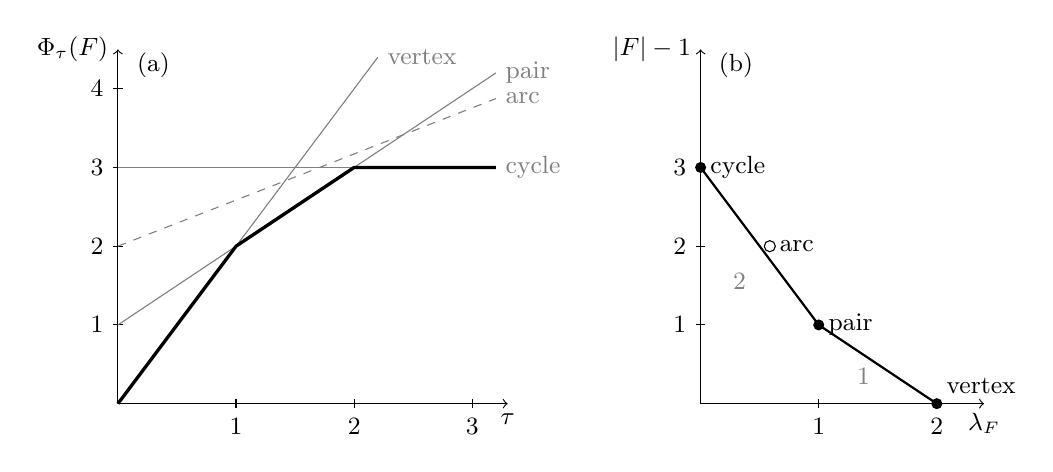
\begin{tikzpicture}[x=1.5cm,y=1.0cm,font=\small]
 \draw[->] (0,0) -- (3.3,0) node[below] {$\tau$};
 \draw[->] (0,0) -- (0,4.5) node[left] {$\Phi_\tau(F)$};
 \foreach \x in {1,2,3} \draw (\x,0.06) -- (\x,-0.06) node[below] {$\x$};
 \foreach \y in {1,2,3,4} \draw (0.04,\y) -- (-0.04,\y) node[left] {$\y$};
 \draw[gray] (0,0) -- (2.2,4.4) node[anchor=west] {vertex};
 \draw[gray] (0,1) -- (3.2,4.2) node[anchor=west] {pair};
 \draw[gray,dashed] (0,2) -- (3.2,{2+0.5858*3.2}) node[anchor=west] {arc};
 \draw[gray] (0,3) -- (3.2,3) node[anchor=west] {cycle};
 \draw[very thick] (0,0) -- (1,2) -- (2,3) -- (3.2,3);
 \node at (0.3,4.3) {(a)};
 \begin{scope}[xshift=7.4cm]
 \draw[->] (0,0) -- (2.4,0) node[below] {$\lambda_F$};
 \draw[->] (0,0) -- (0,4.5) node[left] {$\lvert F\rvert-1$};
 \foreach \x in {1,2} \draw (\x,0.06) -- (\x,-0.06) node[below] {$\x$};
 \foreach \y in {1,2,3} \draw (0.04,\y) -- (-0.04,\y) node[left] {$\y$};
 \draw[thick] (2,0) -- (1,1) -- (0,3);
 \fill (2,0) circle (2pt) node[above right] {vertex};
 \fill (1,1) circle (2pt) node[right] {pair};
 \draw[fill=white] (0.5858,2) circle (2pt) node[right] {arc};
 \fill (0,3) circle (2pt) node[right] {cycle};
 \node[gray] at (1.38,0.35) {$1$};
 \node[gray] at (0.33,1.55) {$2$};
 \node at (0.3,4.3) {(b)};
 \end{scope}
\end{tikzpicture}
\caption{The 4-cycle. (a) The exponents $\Phi_\tau(F)=\tau\lambda_F+\lvert
F\rvert-1$ of the four kinds of faces against $\tau$, and their lower envelope
(bold). The mode sits on the face whose line is lowest, namely a vertex for
$\tau<1$, an adjacent pair for $1<\tau<2$ and the whole cycle for $\tau>2$. The
dashed line of the arc of three states is never lowest. (b) The same faces as points
$(\lambda_F,\lvert F\rvert-1)$, with the lower-left boundary of their convex
hull. The gray numbers are minus the slopes of its edges, the values of $\tau$
where the winner changes (Theorem~\ref{thm:hull}). The arc (open) lies above
the boundary}
\label{fig:C4worked}
\end{figure}

\subsection{Face selection}

We also need an upper bound on a whole face, including near its boundary, where
the local law does not apply. For an irreducible face $F$ put
$V_F=\{\theta\in\R^F:\varrho(A_F-\operatorname{diag}\theta)=0\}$. Each
$\theta\in V_F$ gives an exponential bound with the linear rate
$\alpha\mapsto\langle q-\theta,\alpha\rangle$, and $J_F$ is the supremum of these
linear rates. Indeed, for $u\in(0,\infty)^F$ the vector $\theta=A_Fu/u$
(entrywise) lies in $V_F$, since $u$ is a positive null vector of the irreducible
Metzler matrix $A_F-\operatorname{diag}\theta$ and only its Perron root has a
positive eigenvector. Then $\langle q-\theta,\alpha\rangle$ is the function of $u$
inside the supremum that defines $J_F(\alpha)$. Conversely every $\theta\in V_F$
arises in this way from a positive Perron vector of
$A_F-\operatorname{diag}\theta$. For a field $v\in\R^F$ the vector
$\theta=q-v-\lambda_F(v)\ones$ lies in $V_F$, since
$A_F-\operatorname{diag}\theta=Q_F+\operatorname{diag}v+\lambda_F(v)I$.

\begin{lemma}[a uniform upper bound]\label{lem:upper}
Let $F$ be irreducible with $k=\lvert F\rvert\ge2$, and let $\theta\in V_F$.
There is $C_\theta$, depending on $\theta$, $Q$ and $\mu$ and bounded for $\theta$
in compact subsets of $V_F$, such that for every $n\in\Z_{\ge0}^F$ with
$\supp n=F$ and every $h$ with $hq_{\max}\le\frac12$, the probability that
$X_1,\dots,X_{\lvert n\rvert}$ have composition $n$ is at most
$C_\theta h^{k-1}\exp\bigl(-h\langle n,q-\theta\rangle+C_\theta h^2\lvert
n\rvert\bigr)$.
\end{lemma}

The proof is in Appendix~\ref{app:torus}. The lemma holds for a path of any
length $\lvert n\rvert$, so it also applies to the blocks of a path. With
$\theta=q-v-\lambda_F(v)\ones$ and $\lvert n\rvert=N$ it gives
\begin{equation}\label{eq:upper-field}
 P_N(n)e^{Tv\cdot n/N}\le C_\theta h^{k-1}e^{-T\lambda_F(v)+C_\theta T^2/N}
\end{equation}
for every $n$ with support $F$. For $v=0$ this is the upper half of the rule
$M_F\approx N^{-(k-1)}e^{-T\lambda_F}$ of Section~\ref{sec:worked}, up to a power
of $T$. The next theorem uses the local law and the face maxima of
Section~\ref{sec:secondorder}, which are proved there without it.

\begin{theorem}[first-order face selection]\label{thm:first}
Fix $Q$ and $\mu$.
\begin{enumerate}[(i)]
\item Let $F$ satisfy (H), let $k=\lvert F\rvert$, and let
$\mathcal K\subset\Delta_F^\circ$ be compact. There is $N_0$ such that,
uniformly for $N\ge N_0$, $1\le T\le N^{1/3}$ and $\supp n=F$ with
$n/N\in\mathcal K$,
\[
 \log P_N(n)=-(k-1)L-T\,J_F(n/N)+O_{\mathcal K}(1+\log T).
\]
\item Let $F$ be admissible with components $C_1,\dots,C_r$, and let $k^*$ be
the least size of a component $C_j$ with $\lambda_{C_j}=\lambda_F$. There are
$\kappa$, $T_0$ and $N_0$ such that for $N\ge N_0$ and $T_0\le T\le N^{1/3}$
\begin{align*}
 \log M_F&\ge-(k_F-1)L+(k_F-k^*)\log T-T\lambda_F-\kappa,\\
 \log M_F&\le-(k_F-1)L+(k_F-1)\log T-T\lambda_F+\kappa.
\end{align*}
If $F$ is not admissible, $M_F=0$.
\item Let $T=\tau L$ with $\tau>0$ fixed, and let $\mathcal F_\tau$ be the set
of admissible faces that minimize $\Phi_\tau$. Then
$\log\max_nP_N(n)=-L\min_F\Phi_\tau(F)+O(\log L)$, with the minimum over
admissible faces, and for large $N$ every global mode $\hat n$ has
$\supp\hat n\in\mathcal F_\tau$. This holds for every start $\mu$.
\item If in (iii) every face in $\mathcal F_\tau$ is irreducible, then every
global mode $\hat n$ satisfies $\hat n/N=\alpha^*_F+O(1/L)$ with
$F=\supp\hat n$. This is the case when $Q$ has symmetric support or $\mu$ has
full support (Theorem~\ref{thm:hull}(c)).
\end{enumerate}
\end{theorem}

In words, a composition whose fractions $\alpha$ stay in a compact part of the
open face has probability $N^{-(k-1)}e^{-TJ_F(\alpha)}$ up to a bounded factor
and a power of $T$. The best composition on an admissible face has probability
$N^{-(k_F-1)}e^{-T\lambda_F}$ times a power of $T$ with exponent between $0$ and
$k_F-1$. With $T=\tau L$ the exponent of $N$ is $-\Phi_\tau(F)$, and the mode lies
on a face that minimizes it, whatever the start.

\begin{proof}
(i) For $k=1$ this is~\eqref{eq:vertexmax}, since $J_{\{i\}}=q_i$. For $k\ge2$,
Lemma~\ref{lem:discrete} gives $P_N(n)=N^{-(k-1)}f_T(n/N)(1+O(T^2/N))$. For
$T\ge T_1$ Theorem~\ref{thm:local} gives
$\log f_T(\alpha)=\frac{k-1}2\log T+\log C_F(\alpha)-TJ_F(\alpha)+O_{\mathcal K}(1)$
on $\mathcal K$, and for $1\le T\le T_1$ this holds because $f_T$ and $C_F$ are
positive and continuous on $[1,T_1]\times\mathcal K$. As $\log C_F$ is bounded on
$\mathcal K$, adding $\log N^{-(k-1)}=-(k-1)L$ gives (i).

(ii) Let $F$ be admissible. A path visits each component in one block of
consecutive times (proof of Lemma~\ref{lem:admissible}), and an irreducible face
is one component, with $k^*=k_F$. For the upper bound, Lemma~\ref{lem:upper} (or a
direct count if $\lvert C\rvert=1$) bounds a block of length $N_C$ in the
component $C$ by $O(h^{\lvert C\rvert-1}e^{-h\lambda_CN_C})$, and each of the
$r-1$ switches between blocks gives a factor $h$. As $\lambda_C\ge\lambda_F$, this
gives $M_F=O(h^{k_F-1}e^{-T\lambda_F})$. For the lower bound the path spends about
$N/T$ visits in each component except one of least exit rate, which loses a
bounded factor per component, and we divide by the number of compositions. The
details are in Appendix~\ref{app:first}.

(iii) For large $N$ we have $T_0\le T=\tau L\le N^{1/3}$, and both bounds in (ii)
read $\log M_F=-L\,\Phi_\tau(F)+O(\log L)$ for every admissible face, while
$M_F=0$ for the others. Since $\max_nP_N(n)=\max_FM_F$ over finitely many faces,
the first claim follows. Let $m_\tau=\min_F\Phi_\tau(F)$. An admissible
$F\notin\mathcal F_\tau$ has $\Phi_\tau(F)\ge m_\tau+\varepsilon_0$ for a fixed
$\varepsilon_0>0$, so $M_F\le N^{-m_\tau-\varepsilon_0+o(1)}$, which is smaller
than $\max_nP_N(n)=N^{-m_\tau+o(1)}$ for large $N$. A global mode has positive
probability, so its support is admissible, and hence it lies in $\mathcal F_\tau$.

(iv) By (iii), for large $N$ a global mode $\hat n$ maximizes $P_N$ on its face
$F\in\mathcal F_\tau$, which satisfies (H) by Lemma~\ref{lem:admissible}(b). So
Theorem~\ref{thm:facemax} with $T=\tau L\le N^{1/3}$ gives
$\hat n/N=\alpha^*_F+O(1/L)$.
\end{proof}

For a reducible face we only have the bounds in (ii), and in
Example~\ref{ex:threecycle} the power of $T$ differs from $(k_F-1)/2$.

\begin{remark}[a field]\label{rem:first-field}
Let $v\in\R^d$, put $M_F(T,v)=\max\{P_N(n)e^{Tv\cdot n/N}:\supp n=F\}$ and
$\Phi_{\tau,v}(F)=|F|-1+\tau\lambda_F(v_F)$. On an admissible face,
$Q_F+\operatorname{diag}v_F$ is block triangular in the order of the
components, so $\lambda_F(v_F)=\min_j\lambda_{C_j}(v_{C_j})$. The upper bound in
(ii) holds for $M_F(T,v)$ with $\lambda_F(v_F)$ in place of $\lambda_F$. The proof
in Appendix~\ref{app:first} applies with~\eqref{eq:upper-field} on each block and
the exact weight $e^{hv_iN_j}$ on a block $\{i\}$. For $F$ satisfying (H),
Theorem~\ref{thm:facemax} gives the matching lower bound. If $\mu$ has full
support, a reducible admissible face $F$ has a component $C$ with
$\lambda_C(v_C)=\lambda_F(v_F)$, which is admissible with fewer states, so
$\Phi_{\tau,v}(C)\le\Phi_{\tau,v}(F)-1$. So if $\mu$ has full support, then for
fixed $\tau$ and $v$, (iii)
and (iv) hold for the weighted law with $\Phi_{\tau,v}$ and $\alpha^*_F(v)$, every
face that minimizes $\Phi_{\tau,v}$ is irreducible, and a strict minimizer carries
every maximizer of the weighted law for large $N$.
\end{remark}

\subsection{Reading the winners off a convex hull}

For an admissible face $F$ put $P_F=(\lambda_F,\lvert F\rvert-1)$, and let $S$
be the set of these points. Then $\Phi_\tau(F)=\tau x+y$ at $(x,y)=P_F$. Picture
a line of slope $-\tau$ moving up from far below. The first points of $S$ that
it touches are the winners at $\tau$. For each $\tau>0$ the points of
$\operatorname{conv}S$ where $\tau x+y$ is least form a vertex or an edge of
$\operatorname{conv}S$, and we call the union of these over all $\tau>0$ the
lower-left boundary of $\operatorname{conv}S$. Figure~\ref{fig:C4worked}(b) shows
it for the 4-cycle.

\begin{theorem}[geometry of the winners]\label{thm:hull}
Let $\mathcal F_\tau$ be the set of admissible faces that minimize
$\Phi_\tau$.
\begin{enumerate}[(a)]
\item The lower-left boundary of $\operatorname{conv}S$ is a path whose
vertices lie in $S$. Read from right to left, they are
$v_i=(\lambda^{(i)},y^{(i)})$, $0\le i\le m$, with
$\lambda^{(0)}>\dots>\lambda^{(m)}$ and $y^{(0)}<\dots<y^{(m)}$. Put
$\tau_i=(y^{(i)}-y^{(i-1)})/(\lambda^{(i-1)}-\lambda^{(i)})$ for $1\le i\le m$,
$\tau_0=0$ and $\tau_{m+1}=\infty$. Then $\tau_1<\dots<\tau_m$. For
$\tau_i<\tau<\tau_{i+1}$, $\mathcal F_\tau$ is the set of faces $F$ with
$P_F=v_i$. At $\tau=\tau_i$ it is the set of faces whose point lies on the
closed edge $[v_{i-1},v_i]$.
\item If $0<\tau<\tau'$, $F\in\mathcal F_\tau$ and $G\in\mathcal F_{\tau'}$,
then $\lambda_F\ge\lambda_G$ and $\lvert F\rvert\le\lvert G\rvert$. Both
inequalities are strict when $\mathcal F_\tau\cap\mathcal F_{\tau'}=\emptyset$.
\item If $Q$ has symmetric support, or $\mu$ has full support, then every face
in $\mathcal F_\tau$ is irreducible, for every $\tau>0$.
\end{enumerate}
\end{theorem}

In words, as $\tau$ grows the winners walk up the lower-left boundary of the
hull, from small faces with large exit rates to large faces with small exit
rates, and they change at the values $\tau_i$, minus the slopes of its edges.

\begin{proof}
(a) We study the least value $g(\tau)=\min_{(x,y)\in S}(\tau x+y)$ for $\tau>0$. Each point
$(x,y)$ of $S$ gives the affine function $\tau\mapsto\tau x+y$, whose slope is $x$, and different
points give different functions. So $g$ is a minimum of finitely many affine functions. It is
concave and piecewise affine. Let $\tau_1<\dots<\tau_m$ be the points of $(0,\infty)$ where its
slope changes, and put $\tau_0=0$ and $\tau_{m+1}=\infty$.

\emph{Between two kinks.} On $(\tau_i,\tau_{i+1})$ the function $g$ is affine. The affine
function of a point of $S$ is nowhere below $g$. So if it equals $g$ at one $\tau$ inside this
interval, it equals $g$ on the whole interval. Hence exactly one point of $S$ attains $g$ there.
We call it $v_i=(\lambda^{(i)},y^{(i)})$, and for $\tau_i<\tau<\tau_{i+1}$ the set
$\mathcal F_\tau$ consists of the faces $F$ with $P_F=v_i$. The slope of $g$ on this interval is
$\lambda^{(i)}$. The slope of a concave function decreases, and it changes at each $\tau_i$, so
$\lambda^{(0)}>\dots>\lambda^{(m)}$. By continuity both $v_{i-1}$ and $v_i$ attain $g(\tau_i)$,
namely
\[
\tau_i\lambda^{(i-1)}+y^{(i-1)}=\tau_i\lambda^{(i)}+y^{(i)} .
\]
This is the formula for $\tau_i$ in the statement, and since $\tau_i>0$ it gives
$y^{(i)}>y^{(i-1)}$.

\emph{At a kink.} The points $(x,y)$ of $S$ that attain $g(\tau_i)$ are those on the line
$\tau_ix+y=g(\tau_i)$, which passes through $v_{i-1}$ and $v_i$. Let $(x,y)$ be one of them. For
$\tau$ slightly below $\tau_i$ we have $\tau x+y\ge g(\tau)=\tau\lambda^{(i-1)}+y^{(i-1)}$, with
equality at $\tau=\tau_i$. Subtracting gives $(\tau-\tau_i)(x-\lambda^{(i-1)})\ge0$, so
$x\le\lambda^{(i-1)}$. In the same way, $\tau$ slightly above $\tau_i$ gives
$x\ge\lambda^{(i)}$. So $(x,y)$ lies on the closed edge $[v_{i-1},v_i]$. Conversely every point of
$S$ on this edge lies on the line and so attains $g(\tau_i)$.

\emph{The boundary.} On $\operatorname{conv}S$ the function $\tau x+y$ is least exactly on the
convex hull of the points of $S$ where it is least. By the two steps above this hull is the
vertex $v_i$ for $\tau_i<\tau<\tau_{i+1}$ and the edge $[v_{i-1},v_i]$ for $\tau=\tau_i$. So the
lower-left boundary is the path $v_0\cdots v_m$, and its vertices lie in $S$.

(b) We add two inequalities. Since $F$ wins at $\tau$ and $G$ wins at $\tau'$, we have
$\Phi_\tau(F)\le\Phi_\tau(G)$ and $\Phi_{\tau'}(G)\le\Phi_{\tau'}(F)$. Adding them gives
$(\tau'-\tau)(\lambda_F-\lambda_G)\ge0$, so $\lambda_F\ge\lambda_G$. Then the first inequality
gives $\lvert F\rvert-\lvert G\rvert\le\tau(\lambda_G-\lambda_F)\le0$. If
$\lambda_F=\lambda_G$, the two inequalities give $\lvert F\rvert=\lvert G\rvert$, so
$\Phi_{\tau'}(F)=\Phi_{\tau'}(G)$ and $F\in\mathcal F_{\tau'}$. So if $\mathcal F_\tau$ and
$\mathcal F_{\tau'}$ are disjoint, then $\lambda_F>\lambda_G$, and the first inequality gives
$\lvert F\rvert<\lvert G\rvert$.

(c) With symmetric support every admissible face is irreducible by
Lemma~\ref{lem:admissible}(c). Now let $\mu$ have full support, and let $F$ be admissible and
reducible. Take a component $C$ of $F$ with $\lambda_C=\lambda_F$. It is irreducible with
$\mu(C)>0$, so it is admissible by Lemma~\ref{lem:admissible}(b). It has the same exit rate as
$F$ and fewer states, so $\Phi_\tau(C)\le\Phi_\tau(F)-1$. Hence $F\notin\mathcal F_\tau$.
\end{proof}

Lean checks part (b), the fact that a face with a proper subface of the same exit
rate never wins, and part (a) when the least exit rate of each size decreases
strictly with the size. In that case the vertices of the hull are sizes, and
Lean checks which size wins between consecutive kinks and that consecutive
vertices tie at $\tau_i$. The general path structure in (a) and the ties along
a closed edge are proved only here. A face with small $\lambda_F$ for
its size is a set of states that the chain rarely leaves, a well-separated community. As $\tau$
grows the exit rate counts for more, and the mode moves to larger communities. It need not
grow around its first vertex, and it can move to a disjoint community.
For symmetric $Q$, $\lambda_F$ is the least value of
$\sum_{i<j}q_{ij}(f_i-f_j)^2$, the sum over all pairs in $[d]$, over unit
vectors $f$ supported in $F$ (Rayleigh--Ritz), and it
decreases strictly as a connected face grows, by Lemma~\ref{lem:face-monotone}. Since faces of one size share the term
$\lvert F\rvert-1$, only the faces with the least exit rate of each size can win. Figure~\ref{fig:cycles}(a) shows $S$ for the 6-cycle.

\begin{figure}[t]
\centering
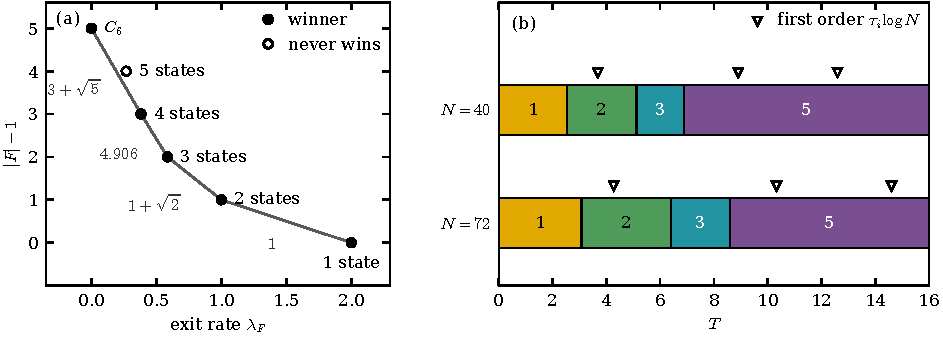
\includegraphics[width=\textwidth]{fig_cycles}
\caption{(a) The points $(\lambda_F,\lvert F\rvert-1)$ of the arcs of the 6-cycle $C_6$ and of $C_6$ itself,
with the lower-left boundary of their hull. The numbers beside the edges are the switch values
$\tau_i$ of Theorem~\ref{thm:hull}. The winners (filled) are the arcs of one to four states and
$C_6$, and the arc of five states (open) never wins. (b) The support size of the exact mode on
$C_5$ with the uniform start, against $T$, at $N=40$ and $N=72$. The mode skips the arc of four
states. The triangles mark the first-order switch points $\tau_i\log N$ with $\tau_i=1$,
$1+\sqrt2$ and $2+\sqrt2$}
\label{fig:cycles}
\end{figure}

\section{The second-order theory}\label{sec:secondorder}

To locate a crossing up to $o(1)$ we need the power of $T$ and the constant in front
of $N^{-(k-1)}e^{-T\lambda_F}$ for every face that satisfies (H). In this section
gradients and Hessians in $\alpha$ are taken in the coordinates
$\alpha'=(\alpha_2,\dots,\alpha_k)$, $|\cdot|$ is the Euclidean norm, and
$q=(q_i)_{i\in F}$.

\subsection{The tilted chain and the constant}\label{sec:tilt}

To find the probability of a composition with fractions $\alpha$ we change the
rates so that $\alpha$ becomes typical. The optimal vector $r_\alpha$ in the
definition of $J_F(\alpha)$ gives a new generator $\widehat Q_\alpha$ on $F$, with
the same switching graph, whose stationary law is exactly $\alpha$. Under it the
visit fractions satisfy a central limit theorem with covariance
$\Gamma_\alpha/T$, and the price of the change of rates is $e^{-TJ_F(\alpha)}$
times boundary factors for the start and the end of the path. The constant
$C_F(\alpha)$ collects these factors and the Gaussian normalization.

\begin{definition}[tilt and constants]\label{def:tilt}
Let $F$ be irreducible with $k\ge2$. For
$\alpha\in\Delta_F^\circ$ let $r_\alpha$ attain the supremum defining
$J_F(\alpha)$ (Proposition~\ref{prop:rate}(b)), and put
$\theta(\alpha)=A_Fr_\alpha/r_\alpha$ and $l_\alpha=\alpha/r_\alpha$
(entrywise). The \emph{tilted generator} is
$\widehat Q_\alpha=R^{-1}(A_F-\operatorname{diag}\theta(\alpha))R$ with
$R=\operatorname{diag}r_\alpha$. With $D=\operatorname{diag}\alpha$ let
\[
Z_\alpha=(\ones\alpha^\top-\widehat Q_\alpha)^{-1}-\ones\alpha^\top,
\qquad\Gamma_\alpha=DZ_\alpha+Z_\alpha^\top D,
\]
and let $\Sigma_\alpha$ be $\Gamma_\alpha$ with the row and column of state
$1$ deleted. Finally let
\[
C_F(\alpha)=\frac{(\mu\cdot r_\alpha)(l_\alpha\cdot\ones)}
{(2\pi)^{(k-1)/2}\sqrt{\det\Sigma_\alpha}},\qquad K_F=C_F(\alpha^*_F).
\]
\end{definition}

For a single state we put $K_{\{i\}}=\mu_i$.
Nothing in Definition~\ref{def:tilt} changes when $r_\alpha$ is scaled, and nothing
in it involves the diagonal of $Q_F$. The objects depend on $A_F$ and $\mu$ only, so a
field does not change them. For $v\in\R^F$ we put $K_F(v)=C_F(\alpha^*_F(v))$, so
that $K_F(0)=K_F$, and $K_{\{i\}}(v)=\mu_i$. Also
$l_\alpha\cdot r_\alpha=1$ and $J_F(\alpha)=\langle q-\theta(\alpha),\alpha\rangle$. Since
$r_\alpha$ minimizes $u\mapsto\sum_{i\ne j}\alpha_iq_{ij}u_j/u_i$, its derivative in $u_j$, which
is $\sum_il_{\alpha,i}q_{ij}-l_{\alpha,j}\theta_j(\alpha)$, vanishes at $r_\alpha$. Hence
\begin{equation}\label{eq:stationary}
l_\alpha^\top\bigl(A_F-\operatorname{diag}\theta(\alpha)\bigr)=0 .
\end{equation}
Also $(A_F-\operatorname{diag}\theta(\alpha))r_\alpha=0$ with $r_\alpha>0$, so $\theta(\alpha)\in
V_F$~\cite{bermanplemmons1994}. So $\widehat Q_\alpha$ is an irreducible generator with the
same off-diagonal zero pattern as $A_F$, and by~\eqref{eq:stationary} its stationary law is
$\alpha$. If $(\ones\alpha^\top-\widehat Q_\alpha)v=0$, multiplying by $\alpha^\top$ gives
$\alpha^\top v=0$, so $\widehat Q_\alpha v=0$. Hence $v$ is a multiple of $\ones$, and
$\alpha^\top v=0$ gives $v=0$. Thus $Z_\alpha$ exists, and
\begin{equation}\label{eq:Zprops}
Z_\alpha\ones=0,\qquad\alpha^\top Z_\alpha=0,\qquad
-\widehat Q_\alpha Z_\alpha=I-\ones\alpha^\top .
\end{equation}
So $\Gamma_\alpha\ones=0$. As $\Gamma_\alpha$ is symmetric, its adjugate is then a multiple of
$\ones\ones^\top$, so deleting another state instead of state $1$ gives the same
$\det\Sigma_\alpha$. At $\alpha^*_F$ the vector $u=r_F$ gives the value $\lambda_F=J_F(\alpha^*_F)$,
so $r_{\alpha^*_F}$ is a multiple of $r_F$, $\theta(\alpha^*_F)=q-\lambda_F\ones$, and
$l_{\alpha^*_F}$ is the matching multiple of $l_F$.

For conductances $c_{ij}=c_{ji}$ on $F$ let
$\tree(c)=\sum_{\mathcal T}\prod_{\{i,j\}\in\mathcal T}c_{ij}$, the sum over
the spanning trees $\mathcal T$ of the complete graph on $F$.

\begin{proposition}[the constant]\label{prop:constant}
Let $F$ be irreducible with $k\ge2$.
\begin{enumerate}[(a)]
\item The maps $\alpha\mapsto\theta(\alpha)$, $J_F(\alpha)$, $\Sigma_\alpha$,
$r_\alpha$ and $l_\alpha$ (with $\sum_ir_{\alpha,i}=1$) are real-analytic on
$\Delta_F^\circ$, $\Sigma_\alpha$ is positive definite, and
$\nabla^2J_F(\alpha)=\Sigma_\alpha^{-1}$. Hence
$\det\Sigma_\alpha\cdot\det\nabla^2J_F(\alpha)=1$ and
$C_F(\alpha)=(\mu\cdot r_\alpha)(l_\alpha\cdot\ones)
\sqrt{\det\nabla^2J_F(\alpha)/(2\pi)^{k-1}}$.
\item Suppose that $\nu_iq_{ij}=\nu_jq_{ji}$ for $i,j\in F$ and some
$\nu\in(0,\infty)^F$. Then $r_\alpha$ is a multiple of $\sqrt{\alpha/\nu}$
and $l_\alpha$ of $\sqrt{\alpha\nu}$, and $\widehat Q_\alpha$ is reversible
with conductances $c_{ij}(\alpha)=\sqrt{\alpha_i\alpha_j}\,q_{ij}\sqrt{\nu_i/\nu_j}$.
Also $J_F(\alpha)=\sum_iq_i\alpha_i-\sum_{i\ne j}c_{ij}(\alpha)$, and
\[
\det\Sigma_\alpha=\frac{2^{k-1}(\prod_i\alpha_i)^2}{\tree(c(\alpha))},\qquad
C_F(\alpha)=\frac{(\mu\cdot r_\alpha)(l_\alpha\cdot\ones)}{(4\pi)^{(k-1)/2}}
\,\frac{\sqrt{\tree(c(\alpha))}}{\prod_i\alpha_i}.
\]
\end{enumerate}
\end{proposition}

\begin{proof}
The proof of (a) is in Appendix~\ref{app:torus} and uses Lemma~\ref{lem:perron}.

(b) We guess the vector $r_\alpha$ and check that the guess is a critical point. Put
$u=\sqrt{\alpha/\nu}$ and $l=\alpha/u=\sqrt{\alpha\nu}$ entrywise. As we saw
before~\eqref{eq:stationary}, the derivative of $\sum_{i\ne j}\alpha_iq_{ij}u_j/u_i$ in $u_j$ is
$\sum_il_iq_{ij}-l_j(A_Fu)_j/u_j$. Here
\[
\sum_il_iq_{ij}=\sum_i\sqrt{\alpha_i\nu_i}\,q_{ij}\qquad\text{and}\qquad
\frac{l_j(A_Fu)_j}{u_j}=\nu_j\sum_iq_{ji}\sqrt{\alpha_i/\nu_i}
=\sum_i\sqrt{\alpha_i\nu_i}\,q_{ij},
\]
where the last step uses $\nu_jq_{ji}=\nu_iq_{ij}$. So the derivative vanishes at $u$. The
function is convex in $\log u$, so its critical point $u$ is a minimizer, and the minimizer is
unique up to a factor (Proposition~\ref{prop:rate}(b)). Hence $r_\alpha$ is a multiple of $u$ and
$l_\alpha$ is the matching multiple of $l$. Then
$\alpha_i(\widehat Q_\alpha)_{ij}=l_iq_{ij}u_j=c_{ij}(\alpha)$ for $i\ne j$, and
$c_{ij}(\alpha)=c_{ji}(\alpha)$ because $q_{ij}\sqrt{\nu_i/\nu_j}=q_{ji}\sqrt{\nu_j/\nu_i}$.
So $\widehat Q_\alpha$ is reversible with these conductances. Also
$\alpha_i\theta_i(\alpha)=l_i(A_Fu)_i=\sum_{j\ne i}c_{ij}(\alpha)$, and
$J_F(\alpha)=\langle q-\theta(\alpha),\alpha\rangle$ gives the formula for $J_F$.

For the determinant we express the quadratic form of $\Sigma_\alpha$ through the Laplacian of the
conductances, namely $\mathcal L=-D\widehat Q_\alpha$. It is symmetric, its off-diagonal entries
are $-c_{ij}(\alpha)$, and $\mathcal L\ones=0$. Fix $\eta\in\R^F$ with $\eta_1=0$, and put
$w=Z_\alpha\eta$ and $\zeta=D\eta-(\alpha\cdot\eta)\alpha$. By~\eqref{eq:Zprops},
$\mathcal Lw=D(I-\ones\alpha^\top)\eta=\zeta$ and $\alpha\cdot w=0$. So
$\eta^\top\Gamma_\alpha\eta=2(D\eta)^\top w=2\zeta^\top w$, where the second step uses
$\alpha\cdot w=0$. Next we remove state $1$. Let $v=w-w_1\ones$,
so that $v_1=0$. Since $\zeta\cdot\ones=0$ and $\mathcal L\ones=0$, we have
$\zeta^\top w=\zeta^\top v$ and $\mathcal Lv=\zeta$. We write primes for the coordinates
$2,\dots,k$, $D'=\operatorname{diag}\alpha'$, and $\mathcal L_{(1)}$ for $\mathcal L$ without row
and column $1$. As $v_1=0$, the rows $2,\dots,k$ of $\mathcal Lv=\zeta$ say that
$\mathcal L_{(1)}v'=\zeta'$, and as $\eta_1=0$ we have $\zeta'=(D'-\alpha'\alpha'^\top)\eta'$. The
matrix-tree theorem~\cite{bollobas1998} gives $\det\mathcal L_{(1)}=\tree(c(\alpha))$, which is
positive because $F$ is irreducible. So $\mathcal L_{(1)}$ is invertible, and
\[
\eta'^\top\Sigma_\alpha\eta'=2\zeta'^\top v'
=2\eta'^\top(D'-\alpha'\alpha'^\top)\mathcal L_{(1)}^{-1}(D'-\alpha'\alpha'^\top)\eta'
\]
for every $\eta'\in\R^{k-1}$. Both matrices are symmetric, hence
$\Sigma_\alpha=2(D'-\alpha'\alpha'^\top)\mathcal L_{(1)}^{-1}(D'-\alpha'\alpha'^\top)$. We take
determinants. The matrix determinant lemma gives
$\det(D'-\alpha'\alpha'^\top)=\prod_{i\ge2}\alpha_i\,(1-\sum_{i\ge2}\alpha_i)=\prod_i\alpha_i$.
So $\det\Sigma_\alpha=2^{k-1}(\prod_i\alpha_i)^2/\tree(c(\alpha))$, and putting this into
Definition~\ref{def:tilt} gives the formula for $C_F(\alpha)$.
\end{proof}

\begin{corollary}[symmetric faces]\label{cor:symface}
Let $F$ satisfy \textup{(H)} with $k\ge2$, and let $Q_F$ be symmetric with constant row sums.
Then $\lambda_F=q_i-\sum_{j\in F\setminus\{i\}}q_{ij}$ for every $i\in F$, $\alpha^*_F$ is uniform
on $F$, and
\[
K_F=\mu(F)\,k^{(k+1)/2}\sqrt{\tree(q_F)}\,(4\pi)^{-(k-1)/2},
\]
where $\tree(q_F)$ is $\tree(c)$ for the conductances $c_{ij}=q_{ij}$, $i,j\in F$.
\end{corollary}

\begin{proof}
The positive vector $\ones$ is a right and left eigenvector of $Q_F$, so it belongs to the
Perron root. So $\lambda_F$ is minus the row sum, $r_F$ and $l_F$ are multiples of $\ones$, and
$\alpha^*_F=\ones/k$.
At $\alpha=\ones/k$, Proposition~\ref{prop:constant}(b) with $\nu=\ones$ gives
$r_\alpha=\ones$, $l_\alpha=\alpha$ and $(\mu\cdot r_\alpha)(l_\alpha\cdot\ones)=\mu(F)$.
Also $c_{ij}(\alpha)=q_{ij}/k$, so $\tree(c(\alpha))=k^{-(k-1)}\tree(q_F)$, and
$\prod_i\alpha_i=k^{-k}$.
\end{proof}

\subsection{The local law and the face maxima}\label{sec:locallaw}

A field $v\in\R^F$ enters the continuum density as an exact factor. By
Lemma~\ref{lem:continuum}, $f_T(\alpha)e^{Tv\cdot\alpha}$ is the density $f_T$ of
the killed matrix $Q_F+\operatorname{diag}v$, which has the same $A_F$ and $\mu$ and
the diagonal $q-v$ in place of $q$. On the lattice the factor is
$e^{Tv\cdot n/N}=e^{h\langle v,n\rangle}$.

\emph{The discrete constant.} Let $F$ be irreducible with $k\ge2$, fix $h_*$ with
$h_*q_{\max}<1$, and let
$(h,\alpha)\in[0,h_*]\times\Delta_F^\circ$. Let $\theta=\theta^{(h)}(\alpha)$ be the
vector of Proposition~\ref{prop:discrete-rate}(b), let $r$ and $l$ be positive right
and left null vectors of $A_F-\operatorname{diag}\theta$ with $l\cdot r=1$, put
$c_h(\alpha)=\sum_i\alpha_i/(1-hq_i+h\theta_i)$, and let
\[
 C^{(h)}_F(\alpha)=c_h(\alpha)\,(\mu\cdot r)(l\cdot\ones)
 \sqrt{\det\nabla^2J^{(h)}_F(\alpha)/(2\pi)^{k-1}} .
\]
Lemma~\ref{lem:discrete-hessian} shows that $\nabla^2J^{(h)}_F$ is positive definite
and that $C^{(h)}_F$ is positive and real-analytic up to $h=0$. At $h=0$ we have
$c_0=1$ and $\theta^{(0)}(\alpha)=\theta(\alpha)$, so $C^{(0)}_F=C_F$ by
Proposition~\ref{prop:constant}(a). For $v\in\R^F$ put
$K^{(h)}_F(v)=C^{(h)}_F(\alpha^{*(h)}_F(v))$ and $K^{(h)}_F=K^{(h)}_F(0)$, and for a
single state $K^{(h)}_{\{i\}}(v)=\mu_i/(1-hq_i)$. At $\alpha^*_F$ the maximizer of
Proposition~\ref{prop:discrete-rate}(b) is $\log r_F$ up to a constant, for every
$h$, by part (c) of that proposition. So
$\theta^{(h)}(\alpha^*_F)=q-\lambda_F\ones$ and
$c_h(\alpha^*_F)=1/(1-h\lambda_F)$.

\begin{theorem}[local law]\label{thm:local}
Let $F$ satisfy \textup{(H)} with $k\ge2$, and let $\mathcal K\subset\Delta_F^\circ$ be
compact.
\begin{enumerate}[(a)]
\item Uniformly for $\alpha\in\mathcal K$, $T\ge1$ and $v\in\R^F$,
\[
f_T(\alpha)e^{Tv\cdot\alpha}=T^{(k-1)/2}C_F(\alpha)e^{-T(J_F(\alpha)-v\cdot\alpha)}\bigl(1+O_{\mathcal K}(1/T)\bigr).
\]
\item Fix $h_*$ with $h_*q_{\max}<1$. Uniformly for $1\le T\le h_*N$,
$\supp n=F$ with $\alpha=n/N\in\mathcal K$, and $v\in\R^F$,
\[
P_N(n)e^{Tv\cdot\alpha}=N^{-(k-1)}T^{(k-1)/2}C^{(h)}_F(\alpha)
e^{-T(J^{(h)}_F(\alpha)-v\cdot\alpha)}\bigl(1+O_{\mathcal K}(1/T)\bigr).
\]
\end{enumerate}
For $F=\{i\}$, $f_T=\mu_ie^{-q_iT}$ and $P_N(Ne_i)=\mu_i(1-hq_i)^{N-1}$.
\end{theorem}

The field cancels from the two sides, so the case $v=0$ is the whole content, and the
error does not depend on $v$. In (b) the ratio of the two sides lies between two
positive constants for all $T$ in the range, so the error is relative.

\emph{Idea of the proof.} The proof is in Appendix~\ref{app:torus}. The
generating function of the words in $H$ is a matrix resolvent, so
Cauchy's formula writes $H$ as an integral over a torus with the radii
$\theta_2(\alpha),\dots,\theta_k(\alpha)$ (Lemma~\ref{lem:torus}).
All the coefficients are nonnegative, so the integrand is largest at the real
point, and a Laplace lemma with a parameter (Lemma~\ref{lem:laplace}) gives the
expansion. The Hessian at the real point comes from the Perron root of a
perturbed generator (Lemma~\ref{lem:perron}), which brings in $\Sigma_\alpha$.
Also $f_T(\alpha)$ is continuous and positive in $(T,\alpha)$, as
$H$ is a convergent power series with some $W(m)>0$ by (H). For (b) the same torus
carries Good's discrete formula, with $e^{t_iz_i}$ replaced by $(1-hq_i+hz_i)^{n_i-1}$
(Lemma~\ref{lem:torus}). In the variable $z$ the integrand is analytic in $h$ up to
$h=0$, where it is the integrand of (a), so one Laplace argument with $(h,\alpha)$ in
the compact set $[0,h_*]\times\mathcal K$ covers $1\le T\le h_*N$. Only for
bounded $T$ does the proof use the comparison of Lemma~\ref{lem:discrete}, to keep
the ratio bounded below.

\begin{lemma}[discrete and continuum]\label{lem:discrete}
Let $F$ satisfy \textup{(H)} with $k\ge2$, and let $\mathcal K\subset\Delta_F^\circ$ be
compact. Uniformly for $\operatorname{supp}n=F$ with $n/N\in\mathcal K$ and
$1\le T\le N^{1/2}$,
$P_N(n)=N^{-(k-1)}f_T(n/N)(1+O_{\mathcal K}(T^2/N))$.
\end{lemma}

The proof is in Appendix~\ref{app:torus}. A field
multiplies both sides by the same factor $e^{Tv\cdot n/N}$. Theorem~\ref{thm:local}(b)
makes this transfer unnecessary for the local law, but the proofs of
Theorem~\ref{thm:local}(b) for bounded $T$ and of Lemma~\ref{lem:derivative} use it.
Together with the restriction identities the local law gives one display for all
faces.

\begin{theorem}[the stratified local law]\label{thm:stratified}
Fix $Q$, a start $\mu$ and $h_*$ with $h_*q_{\max}<1$. Let $F$ satisfy \textup{(H)} with
$|F|=k\ge2$, and let $\mathcal K\subset\Delta_F^\circ$ be compact.
\begin{enumerate}[(a)]
\item Uniformly for $\supp n=F$, $n/N\in\mathcal K$ and $1\le T\le h_*N$,
\[
 -\log P_N(n)=(k-1)L+T\,J^{(h)}_V(n/N)-\frac{k-1}2\log T-\log C^{(h)}_F(n/N)
 +O_{\mathcal K}\Bigl(\frac1T\Bigr).
\]
\item Uniformly for $\supp n=F$, $n/N\in\mathcal K$ and $1\le T\le N^{1/3}$,
\[
 -\log P_N(n)=(k-1)L+T\,J_V(n/N)-\frac{k-1}2\log T-\log C_F(n/N)+O_{\mathcal K}\Bigl(\frac1T+\frac{T^2}N\Bigr).
\]
\end{enumerate}
For a singleton, $-\log P_N(Ne_i)=-\log\mu_i-(N-1)\log(1-hq_i)$, which is
$Tq_i-\log\mu_i+O(T^2/N)$. With $T=\tau L$ the coefficient of $L$ in (b) is
$(k-1)+\tau J_V(n/N)$, the lattice entropy of the face plus $\tau$ times the
Donsker and Varadhan cost of the point.
\end{theorem}

\begin{proof}
(a) This is Theorem~\ref{thm:local}(b) with $v=0$ and
Proposition~\ref{prop:discrete-rate}(a), which replaces $J^{(h)}_F$ by $J^{(h)}_V$
on $\Delta_F$. (b) By Proposition~\ref{prop:discrete-rate}(b) and
Lemma~\ref{lem:discrete-hessian}, $J^{(h)}_F$ and $\log C^{(h)}_F$ are
real-analytic in $(h,\alpha)$ up to $h=0$, so
$TJ^{(h)}_F=TJ_F+O(Th)=TJ_F+O(T^2/N)$ and $\log C^{(h)}_F=\log C_F+O(T/N)$
uniformly on $\mathcal K$. Put this into (a) and replace $J_F$ by $J_V$ on
$\Delta_F$ by Proposition~\ref{prop:restriction}. Part (b) also follows from
Theorem~\ref{thm:local}(a) and Lemma~\ref{lem:discrete}. The singleton case is the
path $i^N$ and~\eqref{eq:vertexmax}.
\end{proof}

For a field $v\in\R^d$ we write $\lambda_F(v)$, $\alpha^*_F(v)$, $K_F(v)$,
$\lambda^{(h)}_F(v)$, $\alpha^{*(h)}_F(v)$ and $K^{(h)}_F(v)$ for the quantities of
$v_F$, and
\[
M_F(T,v)=\max\{P_N(n)e^{Tv\cdot n/N}:\supp n=F\},
\]
so that $M_F(T,0)=M_F$.

\begin{theorem}[face maxima]\label{thm:facemax}
Let $F$ satisfy \textup{(H)}, let $\mathcal V\subset\R^d$ be compact, and fix $h_*$ with
$h_*q_{\max}<1$.
\begin{enumerate}[(a)]
\item If $k\ge2$, then uniformly for $v\in\mathcal V$ and $1\le T\le h_*N$,
\[
M_F(T,v)=N^{-(k-1)}T^{(k-1)/2}K^{(h)}_F(v)e^{-T\lambda^{(h)}_F(v)}\bigl(1+O_{\mathcal V}(1/T)\bigr),
\]
and every maximizer $\hat n$ satisfies $\hat n/N=\alpha^{*(h)}_F(v)+O_{\mathcal V}(1/T)$.
At $v=0$ this reads
$M_F=N^{-(k-1)}T^{(k-1)/2}K^{(h)}_F(1-h\lambda_F)^N(1+O(1/T))$ with
$\hat n/N=\alpha^*_F+O(1/T)$. For $k=1$,
$M_{\{i\}}(T,v)=e^{Tv_i}\mu_i(1-hq_i)^{N-1}=K^{(h)}_{\{i\}}(v)e^{-T\lambda^{(h)}_{\{i\}}(v)}$
exactly.
\item If $k\ge2$, then uniformly for $v\in\mathcal V$ and $1\le T\le N^{1/3}$,
\[
M_F(T,v)=N^{-(k-1)}T^{(k-1)/2}K_F(v)e^{-T\lambda_F(v)}\bigl(1+O_{\mathcal V}(1/T+T^2/N)\bigr),
\]
and every maximizer $\hat n$ satisfies $\hat n/N=\alpha^*_F(v)+O_{\mathcal V}(1/T)$. For
$k=1$, $M_{\{i\}}(T,v)=e^{Tv_i}M_{\{i\}}$ with $M_{\{i\}}$ given by~\eqref{eq:vertexmax}.
In both cases, uniformly for $v\in\mathcal V$ and $1\le T\le N^{1/3}$,
\begin{equation}\label{eq:logmax}
\log M_F(T,v)=-(k-1)L+\tfrac{k-1}2\log T+\log K_F(v)-T\lambda_F(v)+O_{\mathcal V}(1/T+T^2/N).
\end{equation}
\end{enumerate}
\end{theorem}

The constants depend on $\mathcal V$ only through the compact set
$\{\alpha^{*(h)}_F(v):0\le h\le h_*,\ v\in\mathcal V\}$, the bounds of
$\lambda^{(h)}_F$ and $K^{(h)}_F$ on $[0,h_*]\times\mathcal V$, and finitely many
vectors of $V_F$.

\begin{proof}
(a) For $k=1$ the only composition is $Ne_i$. Let $k\ge2$. For
$(h,v)\in[0,h_*]\times\mathcal V$ put
$J^{h,v}(\alpha)=J^{(h)}_F(\alpha)-v\cdot\alpha-\lambda^{(h)}_F(v)$, which is
nonnegative on $\Delta_F$ and vanishes only at $\alpha^{*(h)}_F(v)$, by
Proposition~\ref{prop:discrete-variational}(a) for $h>0$ and
Proposition~\ref{prop:rate}(a) for $h=0$. Put
$X=N^{-(k-1)}T^{(k-1)/2}K^{(h)}_F(v)e^{-T\lambda^{(h)}_F(v)}$, the value that (a)
claims, and write $x=\alpha'-\alpha^{*(h)}_F(v)'$ for the displacement of $\alpha$
from $\alpha^{*(h)}_F(v)$. Below, constants depend only on $Q$, $\mu$, $h_*$ and
$\mathcal V$.

\emph{The balls.} By Proposition~\ref{prop:discrete-variational}(c) the set
$\mathcal A=\{\alpha^{*(h)}_F(v):0\le h\le h_*,\ v\in\mathcal V\}$ is a compact subset
of $\Delta_F^\circ$, and $\lambda^{(h)}_F(v)$ and $\log K^{(h)}_F(v)$ are bounded. By
Proposition~\ref{prop:discrete-rate}(b) and Lemma~\ref{lem:discrete-hessian},
$J^{(h)}_F$ and $\log C^{(h)}_F$ are real-analytic in $(h,\alpha)$ up to $h=0$, with
$\nabla^2J^{(h)}_F$ positive definite, and $J^{h,v}$ has a critical point at
$\alpha^{*(h)}_F(v)$. Taylor's theorem with bounds on the derivatives of order up to
three on $[0,h_*]$ times a compact neighborhood of $\mathcal A$ gives $\rho_0>0$ and
positive constants $c_U$, $C_U$, $C_1$ and $C_3$ with the following properties. The
set $\mathcal K_{\mathcal V}$ of points within $\rho_0$ of $\mathcal A$ lies in
$\Delta_F^\circ$, and for $(h,v)\in[0,h_*]\times\mathcal V$ the ball
$U(h,v)=\{|x|\le\rho_0\}$ satisfies
\[
c_U|x|^2\le J^{h,v}\le C_U|x|^2,\qquad
\bigl|\log(C^{(h)}_F/K^{(h)}_F(v))-g\cdot x\bigr|\le C_1|x|^2
\]
on $U(h,v)$, where $g=\nabla\log C^{(h)}_F(\alpha^{*(h)}_F(v))$ has $|g|\le C_1$.
Also $\log C^{(h)}_F$ is $C_3$-Lipschitz on $\mathcal K_{\mathcal V}$.

\emph{Outside $U(h,v)$.} For $\beta\in\Delta_F$ the definition of $J^{(h)}_F$ and
$((I+hQ_F)u)_i/u_i=1-hq_i+h\theta_i$ with $\theta=A_Fu/u$ give
$J^{(h)}_F(\beta)=\sup_{\theta\in V_F}\sum_i\beta_iL_h(q_i-\theta_i)$, and for fixed
$\theta\in V_F$ the sum is continuous in $(h,\beta)\in[0,h_*]\times\Delta_F$, since
$1-h(q_i-\theta_i)\ge1-h_*q_{\max}$. The set $\mathcal E$ of triples
$(h,v,\beta)\in[0,h_*]\times\mathcal V\times\Delta_F$ with $\beta\notin U(h,v)^\circ$ is
compact, and $J^{h,v}(\beta)$ is positive and lower semicontinuous on it. So
$J^{h,v}\ge3\eta$ on $\mathcal E$ for some $\eta>0$. For each point of $\mathcal E$
the supremum gives $\theta\in V_F$ with
$\sum_i\beta_iL_h(q_i-\theta_i)-v\cdot\beta>\lambda^{(h)}_F(v)+2\eta$, and the same
$\theta$ works near that point. By compactness finitely many vectors
$\theta_j\in V_F$ suffice. Now let $\supp n=F$ with $(h,v,n/N)\in\mathcal E$, and take $j$ that
works there. The bound~\eqref{eq:A-chernoff} with $\theta=\theta_j$, multiplied by
$e^{h\langle v,n\rangle}$, gives, since
$(1-hq_i+h\theta_{j,i})^{n_i}=e^{-hn_iL_h(q_i-\theta_{j,i})}$ with $hn_i=T\beta_i$ for
$\beta=n/N$,
\[
P_N(n)e^{Tv\cdot n/N}\le C(T/N)^{k-1}e^{-T(\lambda^{(h)}_F(v)+2\eta)}=X\cdot O\bigl(T^{(k-1)/2}e^{-2\eta T}\bigr).
\]

\emph{Inside $U(h,v)$.} By Theorem~\ref{thm:local}(b) with
$\mathcal K=\mathcal K_{\mathcal V}$, for $\alpha=n/N\in U(h,v)$,
\begin{equation}\label{eq:insideU}
P_N(n)e^{Tv\cdot n/N}=X\,\tfrac{C^{(h)}_F(\alpha)}{K^{(h)}_F(v)}\,e^{-TJ^{h,v}(\alpha)}(1+E),
\qquad|E|\le C_2/T,
\end{equation}
and $1+E$ lies between two positive constants. For $T\ge2C_1/c_U$ the logarithm of
the two middle factors is at most
\[
g\cdot x+C_1|x|^2-c_UT|x|^2\le g\cdot x-\tfrac{c_UT}2|x|^2\le\frac{|g|^2}{2c_UT},
\]
the maximum of a concave quadratic. So $P_N(n)e^{Tv\cdot n/N}\le X(1+O(1/T))$ on
$U(h,v)$. The bound outside $U(h,v)$ is smaller for large $T$, and hence
$M_F(T,v)\le X(1+O(1/T))$. For the lower bound let $n^0$ have support $F$ and
$|n^0_i-N\alpha^{*(h)}_F(v)_i|<1$ for all $i$, which exists for $N\ge N_0$. Then
$|x|\le k/N$, $C^{(h)}_F(n^0/N)\ge K^{(h)}_F(v)e^{-kC_3/N}$ and
$TJ^{h,v}(n^0/N)\le C_Uk^2T/N^2\le C_Uk^2h_*/N$. Since $1/N\le h_*/T$,
\eqref{eq:insideU} gives $P_N(n^0)e^{Tv\cdot n^0/N}\ge X(1-O(1/T))$.

\emph{Bounded $T$.} Fix $T_2$ such that the two bounds give
$M_F(T,v)/X\in[\frac12,\frac32]$ for $T\ge T_2$. For $1\le T\le T_2$ the same three
steps, with $1+E$ between two positive constants, give $M_F(T,v)/X\in[c,C]$ with
$0<c<C$. This proves the first display, and Proposition~\ref{prop:discrete-variational}(b)
gives the form at $v=0$.

\emph{The maximizer.} Let $\hat n$ be a maximizer with displacement $\hat x$. For
$T\ge T_3$ the bound outside $U(h,v)$ is below $X/2\le P_N(n^0)e^{Tv\cdot n^0/N}$, so
$\hat n/N\in U(h,v)$, and $|E|\le\frac12$ in~\eqref{eq:insideU}. Taking logarithms in
the comparison of $\hat n$ with $n^0$, and using
$\log(C^{(h)}_F/K^{(h)}_F(v))\le C_3|\hat x|$ and $TJ^{h,v}\ge c_UT|\hat x|^2$, we get
\[
c_UT|\hat x|^2\le C_3|\hat x|+\frac{C_4}T
\]
for all $T_3\le T\le h_*N$. Solving the quadratic inequality gives
$|\hat x|\le\bigl(C_3+\sqrt{C_3^2+4c_UC_4}\bigr)/(2c_UT)$. For $1\le T<T_3$ the claim
holds since $|\hat x|$ is bounded.

(b) By Proposition~\ref{prop:discrete-variational}(c) and
Lemma~\ref{lem:discrete-hessian}, uniformly for $v\in\mathcal V$,
$K^{(h)}_F(v)=K_F(v)(1+O(h))$, $\lambda^{(h)}_F(v)=\lambda_F(v)+O(h)$ and
$\alpha^{*(h)}_F(v)=\alpha^*_F(v)+O(h)$. For $T\le N^{1/3}$ we have
$h\le T^2/N\le1/T$ and $Th=T^2/N\le1$. So the value $X$ in (a) is
$N^{-(k-1)}T^{(k-1)/2}K_F(v)e^{-T\lambda_F(v)}(1+O(T^2/N))$, and every maximizer is
within $O(1/T)$ of $\alpha^*_F(v)$. For $k=1$ the formula is the path $i^N$,
and~\eqref{eq:logmax} is the logarithm of the two displays.

\emph{The continuum route to (b).} Part (b) also follows from the proof of (a)
with $J_F$, $C_F$, $K_F(v)$, $\lambda_F(v)$, Theorem~\ref{thm:local}(a) together
with Lemma~\ref{lem:discrete}, and Lemma~\ref{lem:upper} in place of $J^{(h)}_F$,
$C^{(h)}_F$, $K^{(h)}_F(v)$, $\lambda^{(h)}_F(v)$, Theorem~\ref{thm:local}(b)
and~\eqref{eq:A-chernoff}. In~\eqref{eq:insideU} the error is then
$|E|\le C_2(1/T+T^2/N)$, which is at most $\frac12$ for $T_2\le T\le N^{1/3}$ and large $N$.
For bounded $T$ we use that $f_T$ is continuous and positive. In the step that locates the
maximizer the comparison gives $c_UT|\hat x|^2\le C_3|\hat x|+C_4(1/T+T^2/N)$, and
$T^2/N\le1/T$ gives $|\hat x|=O(1/T)$. Proposition~\ref{prop:uniform-facemax} makes this
route uniform over a class of chains.
\end{proof}

\emph{The range of part (b).} The proof of Theorem~\ref{thm:facemax}(b) from part (a)
uses only $Th\le1$ and $h\le1/T$, so it gives the display and the location of the
maximizer for $1\le T\le N^{1/2}$. The same lines give Theorem~\ref{thm:stratified}(b)
for $T\le N^{1/2}$. We state both for $T\le N^{1/3}$, the range of the continuum route,
which needs $T^2/N\le1/T$ to locate the maximizer and is the route that
Proposition~\ref{prop:uniform-facemax} makes uniform. The error $T^2/N$ is not an
artifact of the proof. By the envelope theorem and $L_h(y)=y+hy^2/2+O(h^2)$ for bounded $y$,
uniformly on $\mathcal K$,
\[
 TJ^{(h)}_F(\alpha)=TJ_F(\alpha)+\frac{T^2}{2N}\sum_{i\in F}\alpha_i\bigl(q_i-\theta_i(\alpha)\bigr)^2
 +O\Bigl(\frac{T^3}{N^2}\Bigr),
\]
and $-N\log(1-h\lambda_F)=T\lambda_F+T^2\lambda_F^2/(2N)+O(T^3/N^2)$. The sum
vanishes only where $\theta(\alpha)=q$. Since $\theta$ determines $\alpha$, as the
stationary law of $R^{-1}(A_F-\operatorname{diag}\theta)R$ with $R$ the diagonal of
the Perron vector, this happens only when $\lambda_F=0$ and $\alpha=\alpha^*_F$. So
the continuum exponent $TJ_V$ fails when $T$ is of order $N^{1/2}$, while the
discrete functional absorbs every power of $T/N$ and has no threshold below $h_*N$.
Theorems~\ref{thm:first}(ii) and~\ref{thm:reducible}, which cover reducible faces, and
\ifarxivbuild Theorem~\ref{thm:simplex-crossing}(ii) on the complete graph\else the crossing on the
complete graph in the arXiv version of this paper~\cite{arxivC1}\fi{} are stated for
$T\le N^{1/3}$, and the tie windows of Theorem~\ref{thm:window} for $T$ of order
$L$. We have not extended them.

\subsection{Crossings and tie windows}\label{sec:crossings}

\begin{theorem}[the crossing equation]\label{thm:crossing}
Let $F$ and $G$ satisfy \textup{(H)}, with $\Delta=k_F-k_G\ge1$ and
$\delta=\lambda_G-\lambda_F>0$, and let $D_N(T)=\log M_F-\log M_G$.
\begin{enumerate}[(i)]
\item For large $N$, $D_N$ has a zero in
$[\frac{\Delta}{2\delta}L,\frac{2\Delta}{\delta}L]$.
\item Fix $h_*$ with $h_*q_{\max}<1$. For large $N$, every zero $T_N\in[1,h_*N]$ of
$D_N$ satisfies
\begin{equation}\label{eq:crossing}
\delta T_N+\frac\Delta2\log T_N=\Delta L-\log\frac{K_F}{K_G}
+O\Bigl(\frac1L\Bigr).
\end{equation}
\item All such zeros lie in one interval of length $O(1/L)$, and
\[
T_N=\frac\Delta\delta\Bigl[L-\frac12\log L+b_{FG}\Bigr]
+O\Bigl(\frac{\log L}L\Bigr),\qquad
b_{FG}=-\frac12\log\frac\Delta\delta-\frac1\Delta\log\frac{K_F}{K_G}.
\]
\item For large $N$, $D_N$ has exactly one zero in $[1,h_*N]$.
\end{enumerate}
\end{theorem}

\begin{proof}
\emph{Where the zeros lie.} We show that for large $N$ every zero of $D_N$ in
$[1,h_*N]$ lies in $W=[\frac\Delta{2\delta}L,\frac{2\Delta}\delta L]$. By
Theorem~\ref{thm:facemax}(a) with $v=0$ for $F$, and for $G$ too if $k_G\ge2$,
uniformly for $1\le T\le h_*N$,
\[
D_N(T)=-\Delta L+\Xi_N(T)+\log\frac{K^{(h)}_F}{K^{(h)}_G}+O\Bigl(\frac1T\Bigr),
\qquad\Xi_N(T)=N\log\frac{1-h\lambda_F}{1-h\lambda_G}+\frac\Delta2\log T .
\]
If $G=\{j\}$ this holds by the exact formula $M_G=K^{(h)}_G(1-h\lambda_G)^N$ of
Theorem~\ref{thm:facemax}(a). Since $\lambda_F<\lambda_G\le q_{\max}<1/h$,
\[
\Xi_N'(T)=\frac{\lambda_G}{1-h\lambda_G}-\frac{\lambda_F}{1-h\lambda_F}+\frac\Delta{2T}
=\frac\delta{(1-h\lambda_F)(1-h\lambda_G)}+\frac\Delta{2T}\ge\delta,
\]
and the first term of $\Xi_N$ vanishes at $T=0$, so $\Xi_N(T)\ge\delta T$ for $T\ge1$.
The constants $K^{(h)}_F$ and $K^{(h)}_G$ are continuous and positive in
$h\in[0,h_*]$, so the logarithm of their ratio is bounded. So a zero $T_N$ has
$\Xi_N(T_N)=\Delta L+O(1)$, hence $\delta T_N\le\Delta L+O(1)$ and
$T_N<\frac{2\Delta}\delta L$. For $T\le\frac{2\Delta}\delta L$ we have $Th=O(L^2/N)$,
so $\Xi_N(T)=\delta T+\frac\Delta2\log T+O(L^2/N)$, and
$\Xi_N(\frac\Delta{2\delta}L)=\frac\Delta2L+O(\log L)$. As $\Xi_N$ is increasing,
$T_N>\frac\Delta{2\delta}L$ for large $N$. Also $W\subset[1,N^{1/3}]$ for large $N$.

\emph{On $W$.} We subtract~\eqref{eq:logmax} for $G$ from~\eqref{eq:logmax} for $F$.
Uniformly on $[1,N^{1/3}]$,
\[
D_N(T)=-\Delta L+\Xi(T)+\log\frac{K_F}{K_G}+O\Bigl(\frac1T+\frac{T^2}N\Bigr),
\qquad\Xi(T)=\delta T+\frac\Delta2\log T .
\]
The function $\Xi$ is increasing, with $\Xi'\ge\delta$.

(i) At $T=\frac{\Delta}{2\delta}L$ the display gives $D_N=-\frac\Delta2L+O(\log L)<0$, and at
$T=\frac{2\Delta}\delta L$ it gives $D_N=\Delta L+O(\log L)>0$. For fixed $N$, $M_F$ is a maximum
of finitely many polynomials in $h$, and it is positive because $F$ is admissible. The same holds
for $G$. So $D_N$ is continuous and has a zero in between.

(ii) Let $T_N\in[1,h_*N]$ be a zero. By the first step $T_N\in W$, so $T_N$ is of
order $L$, the error term of the display is $O(1/T_N+T_N^2/N)=O(1/L)$, and
$D_N(T_N)=0$ is~\eqref{eq:crossing}.

(iii) Let $T^\circ$ be the solution of $\Xi(T^\circ)=\Delta L-\log(K_F/K_G)$. By (ii) every zero
has $\Xi(T_N)=\Xi(T^\circ)+O(1/L)$, and $\Xi'\ge\delta$, so every zero is within $O(1/L)$ of
$T^\circ$. To solve for $T^\circ$, we use $T^\circ=\frac\Delta\delta L+O(\log L)$, so
$\log T^\circ=\log L+\log\frac\Delta\delta+O(\log L/L)$. Putting this into
$\delta T^\circ=\Delta L-\frac\Delta2\log T^\circ-\log(K_F/K_G)$ and dividing by $\delta$ gives
the explicit form.

(iv) By the first step, for large $N$ every zero in $[1,h_*N]$ lies in $W$. We show that $D_N$ is strictly increasing
on $W$. For fixed $N$, $M_F$ is the maximum of the finitely many polynomials $T\mapsto P_N(n)$
with $\supp n=F$ that are not identically zero. By Lemma~\ref{lem:runs} each term of such a
polynomial is either zero for all $h$ or positive for all $0<h<1/q_{\max}$, so these polynomials
are positive on $W$. So $\log M_F$ has at each $T\in W$ a right
derivative, the largest $\partial_T\log P_N(n)$ over the maximizers $n$ at $T$, and a left
derivative, the least of them. By Theorem~\ref{thm:facemax} every maximizer has
$n/N=\alpha^*_F+O(1/L)$ on $W$. So for large $N$ it lies in a closed ball
$\mathcal K\subset\Delta_F^\circ$ around $\alpha^*_F$, and $J_F(n/N)=\lambda_F+O(1/L)$, since
$J_F$ is smooth on $\mathcal K$ with $J_F(\alpha^*_F)=\lambda_F$. Lemma~\ref{lem:derivative}
then gives both one-sided derivatives of $\log M_F$ as $-\lambda_F+O(1/L)$ on $W$. The same
holds for $G$ if $k_G\ge2$. If $G=\{j\}$, then $\log M_G=\log\mu_j+(N-1)\log(1-hq_j)$ has the
derivative $-(N-1)q_j/(N(1-hq_j))=-\lambda_G+O(L/N)$. So both one-sided derivatives of $D_N$
are $\delta+O(1/L)\ge\delta/2$ on $W$ for large $N$. A continuous function whose right
derivative is positive at every point of an interval is strictly increasing there. So $D_N$
has at most one zero in $W$, and by (i) it has one.
\end{proof}

On the $4$-cycle at $N=10^{14}$ the explicit form in (iii) differs from the root
of~\eqref{eq:crossing} without its error term by $0.035$ for a vertex against a pair and by
$0.087$ for a pair against the cycle, the two crossings that carry the mode. So computations
should solve~\eqref{eq:crossing}.

At a switch value $\tau^*=\tau_i$ of Theorem~\ref{thm:hull}(a) several faces minimize
$\Phi_{\tau^*}$, sometimes more than two, as all faces do at $\tau^*=1$ for the
complete graph $Q=J-dI$, where $\lambda_F=d-|F|$\ifarxivbuild{} (Corollary~\ref{cor:paperB})\fi. Then the competition plays out in a window $T=\tau^*(L-\frac12\log L+t)$ with $t$ of
order $1$. In this window each tied face has a line $\ell_F(t)$, and the mode
follows the highest line.

\begin{theorem}[tie windows]\label{thm:window}
Fix $\tau^*>0$. Let $m^*$ be the least value of $\Phi_{\tau^*}$ over the
admissible faces and $\mathcal F^*$ the set of minimizers. Assume that every
face in $\mathcal F^*$ is irreducible. By Theorem~\ref{thm:hull}(c) this holds
if $Q$ has symmetric support or $\mu$ has full support. Put $T=\tau^*(L-\frac12\log L+t)$, and for
$F\in\mathcal F^*$ let
$\ell_F(t)=\log K_F+\frac{k_F-1}2\log\tau^*-\tau^*\lambda_Ft$ and
$E(t)=\max_{G\in\mathcal F^*}\ell_G(t)$. The function $E$ is convex and piecewise linear. We call
the finitely many points where its slope changes the \emph{kinks} of $E$, and we write $t_j$ for
them.
\begin{enumerate}[(i)]
\item Uniformly for $t$ in compact sets, for $F\in\mathcal F^*$,
$\log M_F=-m^*L+\frac{m^*}2\log L+\ell_F(t)+O(\log L/L)$.
\item There are $\varepsilon_1,\varepsilon_0>0$ such that for large $N$ and
$|T/L-\tau^*|\le\varepsilon_1$, every admissible $F\notin\mathcal F^*$ has
$M_F\le N^{-\varepsilon_0}\max_{G\in\mathcal F^*}M_G$.
\item There are $\varepsilon,t_0>0$ such that the following holds for large $N$. If
$t_0\le t\le\varepsilon L$, then every global mode lies on a face $F\in\mathcal F^*$ with
$\ell_F=E$ on $[t_0,\infty)$. If $-\varepsilon L\le t\le-t_0$, then every global mode lies on a
face $F\in\mathcal F^*$ with $\ell_F=E$ on $(-\infty,-t_0]$. A face of the first kind has the
least $\lambda_F$ in $\mathcal F^*$, and a face of the second kind has the largest.
\end{enumerate}
The numbers $\varepsilon_0$, $\varepsilon_1$, $\varepsilon$ and $t_0$ depend only on $Q$,
$\mu$ and $\tau^*$.
Consequently the following holds for every $\eta>0$ and large $N$. If $|t|\le\varepsilon L$ and
$t$ is at distance at least $\eta$ from every kink of $E$, then every global mode lies on a face
whose line equals $E$ near $t$. So for $|t|\le\varepsilon L$ the line of the face that carries
the global mode changes only at $T=\tau^*(L-\frac12\log L+t_j)+o(1)$, where $t_j$ runs over the
kinks of $E$, and it changes near each kink. Coincident lines do not distinguish
their faces at this order.
\end{theorem}

\begin{proof}
Every $F\in\mathcal F^*$ is admissible and irreducible, so it satisfies (H) by
Lemma~\ref{lem:admissible}(b). We first put $T$ into~\eqref{eq:logmax}. Write
$T=\tau^*L(1+y)$ with $y=(t-\frac12\log L)/L$, so that $|y|\le\frac12$ for $|t|\le L/4$ and
large $N$. Then $\log T=\log\tau^*+\log L+\log(1+y)$ and
$T\lambda_F=\tau^*\lambda_F(L-\frac12\log L+t)$, and the error term of~\eqref{eq:logmax} is
$O(1/L)$. Since $\tau^*\lambda_F+k_F-1=m^*$, we get, uniformly for $|t|\le L/4$,
\begin{equation}\label{eq:windowline}
\log M_F=-m^*L+\tfrac{m^*}2\log L+\ell_F(t)+\tfrac{k_F-1}2\log(1+y)+O(1/L)
\qquad(F\in\mathcal F^*).
\end{equation}

(i) For $t$ in a compact set, $y=O(\log L/L)$, so $\log(1+y)=O(\log L/L)$
in~\eqref{eq:windowline}.

(ii) Let $g>0$ be the least value of $\Phi_{\tau^*}(F)-m^*$ over the admissible
$F\notin\mathcal F^*$. If there is no such face, (ii) says nothing, and we put $g=1$. Put
$\varepsilon_1=\min\bigl(\tau^*/2,\,g/(4q_{\max}+4)\bigr)$. If $|T/L-\tau^*|\le\varepsilon_1$, then
$\frac12\tau^*L\le T\le\frac32\tau^*L$, so for large $N$ we are in the range of
Theorem~\ref{thm:first}(ii) and $\log T=O(\log L)$. Take an admissible $F\notin\mathcal F^*$ and
any $G\in\mathcal F^*$. Since $0\le\lambda_F,\lambda_G\le q_{\max}$
(Section~\ref{sec:notation}), $\Phi_\tau(F)-\Phi_\tau(G)$ has slope at most $q_{\max}$ in
absolute value, and it is at least $g$ at $\tau^*$. So it is at least $g/2$ for
$|\tau-\tau^*|\le\varepsilon_1$. With $\tau=T/L$ the
upper bound of Theorem~\ref{thm:first}(ii) for $F$ and the lower bound for $G$ give
$\log M_F-\log M_G\le-(\Phi_\tau(F)-\Phi_\tau(G))L+O(\log L)\le-\frac g4L$ for large $N$. So (ii)
holds with $\varepsilon_0=g/4$.

(iii) Take $\varepsilon=\min(\frac14,\varepsilon_1/(2\tau^*))$. Then for $|t|\le\varepsilon L$
and large $N$ we have $|T/L-\tau^*|=\tau^*|y|\le\varepsilon_1$, so (ii) applies and no global
mode lies on a face outside $\mathcal F^*$. It remains to compare the tied faces. Let $t_0\ge1$
be larger than every $|t_j|$, so that $E$ is a single line on $[t_0,\infty)$. Let
$F\in\mathcal F^*$ have this line, and let $G\in\mathcal F^*$ have another line. We show that
$M_F>M_G$ for $t_0\le t\le\varepsilon L$ if $t_0$ and $N$ are large. Since $\ell_F\ge\ell_G$
on $[t_0,\infty)$, the slopes satisfy $\lambda_F\le\lambda_G$. As both faces are tied,
\[
\Delta=k_F-k_G=\tau^*(\lambda_G-\lambda_F)\ge0 .
\]
There are two cases.

First let $\Delta=0$. Then the two lines are parallel, and $\ell_F-\ell_G=\log(K_F/K_G)>0$. The
terms with $\log(1+y)$ in~\eqref{eq:windowline} are the same for $F$ and $G$, so
$\log(M_F/M_G)=\log(K_F/K_G)+O(1/L)>0$ for large $N$.

Now let $\Delta>0$. Then $\ell_F(t)-\ell_G(t)=\Delta t+\ell_F(0)-\ell_G(0)$,
and~\eqref{eq:windowline} gives
\[
\log\frac{M_F}{M_G}=\Delta t+\ell_F(0)-\ell_G(0)+\frac\Delta2\log(1+y)+O\Bigl(\frac1L\Bigr).
\]
For large $N$ and $t\ge1$ we have $|\log(1+y)|\le2|y|\le(2t+\log L)/L\le t/2$. So the right
side is at least $\frac34\Delta t-C$, which is positive for $t\ge t_0$ once $t_0$ is large.

So for $t_0\le t\le\varepsilon L$ every global mode lies on a face whose line is $E$ on
$[t_0,\infty)$. The slope of $\ell_F$ is $-\tau^*\lambda_F$, and $E$ follows the line of largest
slope on the far right, so such a face has the least $\lambda_F$ in $\mathcal F^*$. The case
$t\le-t_0$ is the same with the signs reversed.

\emph{The consequence.} Fix $\eta>0$ and let
$S_\eta=[-t_0,t_0]\setminus\bigcup_j(t_j-\eta,t_j+\eta)$. For $G\in\mathcal F^*$ the function
$E-\ell_G$ is convex, piecewise linear and nonnegative, with kinks only at kinks of $E$. So on
each interval of $S_\eta$ either $\ell_G=E$ or $E-\ell_G\ge g_\eta$ for some $g_\eta>0$. Let
$t\in S_\eta$ and $\ell_F(t)=E(t)$. By (i), every $G\in\mathcal F^*$ whose line is not $E$ near
$t$ has $\log(M_F/M_G)\ge g_\eta-O(\log L/L)>0$, and by (ii) the faces outside $\mathcal F^*$
are smaller still. With (iii) for $t_0\le|t|\le\varepsilon L$ this gives the claim, and the line
does change near each kink, since $E$ is a different line on its two sides.
\end{proof}


\begin{corollary}[where the mode changes]\label{cor:mode-changes}
Let $Q$ have symmetric support or $\mu$ full support. Let $v_0,\dots,v_m$ and
$\tau_1<\dots<\tau_m$ be the vertices and switch values of Theorem~\ref{thm:hull}(a), and
assume that no point of $\mathcal S$ other than $v_{i-1}$ and $v_i$ lies on the edge
$[v_{i-1},v_i]$, for $1\le i\le m$. Put $\Delta_i=y^{(i)}-y^{(i-1)}$ and
$\delta_i=\lambda^{(i-1)}-\lambda^{(i)}$, let $K^{(i)}$ be the largest $K_F$ over the faces
$F$ with $P_F=v_i$, and let $T_{N,i}$ be the root of
$\delta_iT+\frac{\Delta_i}2\log T=\Delta_iL-\log(K^{(i)}/K^{(i-1)})$. Fix $0<a<b$. There are
$C$ and $N_0$ such that for $N\ge N_0$ and every $T\in[aL,bL]$ with $|T-T_{N,j}|\ge C/L$ for
all $j$, every global mode $\hat n$ has $P_{\supp\hat n}=v_i$, where $i$ is the number of $j$
with $T_{N,j}<T$.
\end{corollary}

\begin{proof}
By Theorem~\ref{thm:hull}(a) each face whose point lies on the lower-left boundary belongs to
some $\mathcal F_\tau$, so it satisfies (H) by Theorem~\ref{thm:hull}(c) and
Lemma~\ref{lem:admissible}(b). Let $\mathbb F_i$ be the set of faces $F$ with $P_F=v_i$, and
$M^{(i)}=\max_{F\in\mathbb F_i}M_F$. These faces share $|F|-1=y^{(i)}$ and
$\lambda_F=\lambda^{(i)}$. So for $T$ of order $L$,~\eqref{eq:logmax} gives
$\log(M^{(i)}/M^{(i-1)})=\Xi_i(T)-\Xi_i(T_{N,i})+O(1/L)$ with
$\Xi_i(T)=\delta_iT+\frac{\Delta_i}2\log T$, and $\Xi_i'\ge\delta_i$. Also
$T_{N,i}=\tau_iL+O(\log L)$. Put $\tau_0=0$ and $\tau_{m+1}=\infty$.

\emph{Near a switch value.} By Theorem~\ref{thm:hull}(a) and the assumption,
$\mathcal F_{\tau_i}=\mathbb F_{i-1}\cup\mathbb F_i$. Theorem~\ref{thm:window}(ii) with
$\tau^*=\tau_i$ gives $\varepsilon_1>0$ such that for large $N$ and $|T/L-\tau_i|\le\varepsilon_1$
no face outside $\mathbb F_{i-1}\cup\mathbb F_i$ carries a global mode. We shrink
$\varepsilon_1$ below a third of every gap $\tau_{j+1}-\tau_j$. Then this window contains
$T_{N,i}$ and no other $T_{N,j}$, and by the display there is $C$ such that the global modes lie
in $\mathbb F_i$ for $T\ge T_{N,i}+C/L$ and in $\mathbb F_{i-1}$ for $T\le T_{N,i}-C/L$.

\emph{Between switch values.} Let $J\subset(\tau_i,\tau_{i+1})$ be compact. For $\tau\in J$ only
$v_i$ attains the least value of $\Phi_\tau$ on $\mathcal S$. So $\Phi_\tau(F)-\Phi_\tau(G)\ge g_J>0$
for $\tau\in J$, $G\in\mathbb F_i$ and every admissible $F$ with $P_F\ne v_i$. The bounds of
Theorem~\ref{thm:first}(ii), with $k^*=k_G$ for the irreducible face $G$, give
$\log M_F-\log M_G\le-g_JL+(d-1)\log T+2\kappa<0$ for $T/L\in J$ and large $N$. So every
global mode lies in $\mathbb F_i$, and no $T_{N,j}$ lies in $LJ$. Finitely many windows and
intervals $J$ cover $[a,b]$.
\end{proof}

The equation for $T_{N,i}$ is~\eqref{eq:crossing} for a face of largest constant on each side,
so Theorem~\ref{thm:crossing}(iii) gives $T_{N,i}$ explicitly. If three or more points of
$\mathcal S$ lie on one edge, Theorem~\ref{thm:window} locates the changes only up to $o(1)$. At a
kink of $E$ where the line of $G$ gives way to that of $F$, $\Delta=\tau^*\delta$ and
$t_j=b_{FG}$, so the kink is where Theorem~\ref{thm:crossing}(iii) puts the crossing of $F$ and
$G$. The coefficient $\frac12$ of $\log\log N$ comes from the power $T^{(k-1)/2}$ in
Theorem~\ref{thm:facemax}, so it needs only (H).

\subsection{A reducible face}\label{sec:reducible}

The best composition of a reducible face can visit a state only once, with no
Gaussian window in that direction. Then the coefficient $\frac12$ of
Theorem~\ref{thm:crossing} can fail, and in the next example it is $1$ and then $0$, as
Corollary~\ref{cor:reducible-crossing} predicts.

\begin{example}[a directed $3$-cycle]\label{ex:threecycle}
Let $d=3$, $q_{12}=b>2$, $q_{23}=q_{31}=1$, all other rates $0$, and
$\mu_1=1$. From state $1$ the chain moves only along $1\to2\to3\to1$, so the
admissible faces are $\{1\}$, $\{1,2\}$ (reducible, $\lambda=1$) and
$\{1,2,3\}$ (irreducible, $\lambda=0$).
\begin{enumerate}[(i)]
\item Exactly $M_{\{1\}}=(1-bh)^{N-1}$ and $M_{\{1,2\}}=bh(1-h)^{N-2}$, and the latter is
attained only at $n=(1,N-1,0)$. For the full face,
$\alpha^*=(1,b,b)/(1+2b)$ and $K_{\{1,2,3\}}=(1+2b)^2/(2\sqrt3\,\pi b)$.
\item The equation $M_{\{1\}}=M_{\{1,2\}}$ has exactly one root $T^{(1)}_N$ with $bh<1$, and
$T^{(1)}_N=\frac1{b-1}[L-\log L+\log\frac{b-1}b]+O(\log L/L)$. The coefficient of
$\log\log N$ in the bracket is $1$.
\item Every root $T\in[L/2,2L]$ of $M_{\{1,2\}}=M_{\{1,2,3\}}$ satisfies
$T=L+\log\frac{2\sqrt3\,\pi b^2}{(1+2b)^2}+O(1/L)$, so the coefficient of
$\log\log N$ is $0$.
\end{enumerate}
\end{example}

\begin{proof}[Proof]
(i) A path with support $\{1,2\}$ is $1^{n_1}2^{n_2}$, of probability
$(1-bh)^{n_1-1}\,bh\,(1-h)^{n_2-1}$. Moving one visit from state $2$ to state $1$
multiplies it by $(1-bh)/(1-h)<1$, so the maximum is at $n_1=1$. On the full face $Q$
is a generator, so $\lambda=0$, $r=\ones$, $l=\alpha^*$ and $\alpha^*$ is the stationary law
$(1,b,b)/(1+2b)$. So $(\mu\cdot r)(l\cdot\ones)=1$ and
$K_{\{1,2,3\}}=(2\pi)^{-1}(\det\Sigma_{\alpha^*})^{-1/2}$. By the inequality of the
arithmetic and geometric means, the infimum of
$b\alpha_1u_2/u_1+\alpha_2u_3/u_2+\alpha_3u_1/u_3$ over $u>0$ is $3\phi(\alpha)$ with
$\phi(\alpha)=(b\alpha_1\alpha_2\alpha_3)^{1/3}$. So
$J_V(\alpha)=b\alpha_1+\alpha_2+\alpha_3-3\phi(\alpha)$ by~\eqref{eq:JV}, and by
Proposition~\ref{prop:constant}(a), $\det\Sigma_{\alpha^*}$ is the inverse of the determinant
of the Hessian of $J_V$ in $(\alpha_2,\alpha_3)$ at $\alpha^*$. In all three coordinates the
Hessian of $-3\phi$ is $\phi D^{-1}(I-\frac13\ones\ones^\top)D^{-1}$ with
$D=\operatorname{diag}\alpha$. At $\alpha^*=(c,bc,bc)$ with $c=1/(1+2b)$ we have $\phi=bc$, and
the substitution $\alpha_1=1-\alpha_2-\alpha_3$ gives the Hessian
\[
\frac{1+2b}{3b}\begin{pmatrix}2b^2+2b+2&2b^2+2b-1\\2b^2+2b-1&2b^2+2b+2\end{pmatrix},
\]
whose determinant is $(1+2b)^4/(3b^2)$. Hence $\det\Sigma_{\alpha^*}=3b^2/(1+2b)^4$, which
gives the value of $K_{\{1,2,3\}}$.

(ii) The function $\log(M_{\{1,2\}}/M_{\{1\}})=\log(bh)+(N-2)\log(1-h)-(N-1)\log(1-bh)$
has the derivative $1/h-(N-2)/(1-h)+(N-1)b/(1-bh)>0$ in $h$, since $b>1$ and
$1-bh<1-h$. It tends to $-\infty$ as $h\to0$ and to $+\infty$ as $bh\to1$, so it has
exactly one zero. Its expansion $\log b+\log T-L+(b-1)T+O(T^2/N)$ gives
$(b-1)T+\log T=L-\log b+O(T^2/N)$ at the zero, and with $\log T=\log L-\log(b-1)+O(\log L/L)$
this gives the formula.

(iii) For the full face $k=3$, so Theorem~\ref{thm:facemax} gives
$\log M_{\{1,2,3\}}=-2L+\log T+\log K_{\{1,2,3\}}+O(1/L)$ on $[L/2,2L]$, with the same
power $T^1$ as $\log M_{\{1,2\}}=\log b+\log T-L-T+O(T^2/N)$. So $\log T$ cancels, and
equating the two gives $T=L+\log b-\log K_{\{1,2,3\}}+O(1/L)$.
\end{proof}


\subsection{Face maxima uniformly over a class}\label{sec:uniform-class}

The constants of Theorem~\ref{thm:facemax} depend on $Q$ and $\mu$. We make them
uniform over a compact class of reversible chains on a fixed graph. This is a forward
statement about the face maxima, and the companion paper~\cite{paperC2} uses it to make its
finite-horizon recovery uniform over such a class.

Fix a connected graph $\mathcal G=([d],\mathcal E)$, numbers $0<w_*\le R$ and
$0<\mu_*\le1/d$, and a compact set $\mathcal V\subset\R^d$ of fields. A generator $Q$ is
\emph{on $\mathcal G$} if $q_{ij}>0$ exactly when $\{i,j\}\in\mathcal E$. For a reversible
irreducible $Q$ with stationary law $\pi$ put $w_{ij}=q_{ij}q_{ji}$ and
$S_V=D_{\sqrt\pi}(-Q)D_{\sqrt\pi}^{-1}$, with $D_x=\operatorname{diag}x$, the matrix $S_F$ of
Proposition~\ref{prop:variational} for $F=V$. It is symmetric, with diagonal $q_i$ and
the entries $-\sqrt{w_{ij}}$ on edges. Let $\mathcal C$ be the set of reversible
irreducible generators on $\mathcal G$ with $\|S_V\|_2\le R$ and $\sqrt{w_{ij}}\ge w_*$ on
every edge, and let $\mathcal M$ be the set of starts with $\min_i\mu_i\ge\mu_*$. We use
$M_F(T,v)$, $\alpha^*_F(v)$ and $K_F(v)$ as defined before Theorem~\ref{thm:facemax}.

\begin{proposition}[uniform face maxima on the class]\label{prop:uniform-facemax}
Let $\mathcal G$ induce a connected graph on the face $F$, with $k=|F|\ge2$. There are
$N_0$ and $C$, depending only on $\mathcal G$, $R$, $w_*$, $\mu_*$ and $\mathcal V$, such that for all
$Q\in\mathcal C$, $\mu\in\mathcal M$ and $v\in\mathcal V$ the following hold.
\begin{enumerate}[(a)]
\item For all $N\ge2$ and $T>0$ with $TR\le N/2$,
$M_F(T,v)\le C(T/N)^{k-1}e^{-T\lambda_F(v)+CT^2/N}$.
\item For $N\ge N_0$ and $1\le T\le N^{1/3}$, we have $C^{-1}\le K_F(v)\le C$ and
\[
 M_F(T,v)=K_F(v)\,N^{-(k-1)}T^{(k-1)/2}e^{-T\lambda_F(v)}(1+E),\qquad
 |E|\le C\Bigl(\frac1T+\frac{T^2}N\Bigr).
\]
\end{enumerate}
For a singleton, $M_{\{i\}}(T,v)=\mu_i(1-Tq_i/N)^{N-1}e^{Tv_i}$ exactly.
\end{proposition}

\begin{proof}
For fixed $(Q,\mu)$, part (b) is Theorem~\ref{thm:facemax}(b) with the compact
set $\mathcal V$ of fields, whose constants already do not depend on
$v\in\mathcal V$. We use its continuum route, given at the end of the proof of
Theorem~\ref{thm:facemax}. Part (a) is~\eqref{eq:upper-field}, that is, Lemma~\ref{lem:upper}
with the Perron tilt $\theta=q-v-\lambda_F(v)\ones\in V_F$, and the singleton is
the path $i^N$. It remains to show that no constant depends on $(Q,\mu)$ either.

\emph{The parameter set is compact.} Let $\mathcal P=\mathcal C\times\mathcal M\times\mathcal V$.
Since $S_V$ is symmetric and similar to $-Q$, it is positive semidefinite, so
$0\le q_l\le R$ for every $l$ and $\sqrt{w_{ij}}\le R$ on every edge.
On an edge $q_{ij}\ge w_*^2/R$, since $q_{ij}q_{ji}\ge w_*^2$ and $q_{ji}\le R$, and off the
edges $q_{ij}=0$. Reversibility is the closed condition of Kolmogorov on cycle products,
and $\|S_V\|_2\le R$ is closed since $\pi$ is continuous. So $\mathcal P$ is compact, and
every connected face is irreducible for every $Q\in\mathcal C$.

\emph{Joint regularity.} The Perron root is simple, so $\lambda_F(v)$, the normalized
Perron vectors and $\alpha^*_F(v)$ are real-analytic in $(Q,v)$. The proof of
Proposition~\ref{prop:constant}(a), run with $Q$ as an extra variable, makes
$\theta(\alpha)$, $r_\alpha$, $l_\alpha$, $\Sigma_\alpha$, $J_F$ and $C_F$ real-analytic in
$(\alpha,Q)$, and $C_F$ is linear in $\mu$. So $K_F(v)$ is continuous and positive on
$\mathcal P$, which gives its bounds, and there is $\varepsilon_0>0$ with
$\alpha^*_{F,i}(v)\ge2k\varepsilon_0$ on $\mathcal P$. Put
$\mathcal K_0=\{\alpha\in\Delta_F:\alpha_i\ge\varepsilon_0\ \forall i\}$.

\emph{The constants.} They are the following, and each is continuous on $\mathcal P$ or on
$\mathcal P\times\mathcal K_0$, or comes from a compactness argument run there.
(i) The constant $C_\theta$ of Lemma~\ref{lem:upper} is built from the factor $b(z')$ of
Lemma~\ref{lem:torus}. This factor is continuous where the
radius condition~\eqref{eq:A-radii} holds strictly, as it does on $V_F$. So it is continuous along the Perron tilt.
(ii) In Theorem~\ref{thm:local}(a) the Perron root in~\eqref{eq:A-radii} at $\theta'(\alpha)$ is
continuous and negative on $\mathcal P\times\mathcal K_0$, so one radius margin serves, and
Lemma~\ref{lem:laplace} applies on the compact space $\mathcal P\times\mathcal K_0$, since
the matrix $\mathcal J$ of Appendix~\ref{app:torus} is continuous and positive definite and
$\chi(\alpha,0)=(\mu\cdot r_\alpha)(l_\alpha\cdot\ones)\prod_{i\ge2}\theta_i(\alpha)/\alpha_1$ is
continuous and positive.
(iii) Step~3 of the proof of Lemma~\ref{lem:discrete} needs only $\Upsilon(1)\le CT$, with $C$
uniform on $\mathcal P\times\mathcal K_0$, and we prove this directly. The upper bound
$H_e(T\alpha)\le e^{k-1}b(\theta')\prod_{i\ge2}\theta_i\,e^{eT\langle\alpha,\theta\rangle}$ of that
step, with $\theta=\theta(\alpha)$, has a constant that is continuous on
$\mathcal P\times\mathcal K_0$ by (i). For the lower bound take a walk $c^0$ in $\mathcal G$ through
every state of $F$ with at most $2k-1$ letters, for instance along a depth-first search of a
spanning tree of the graph that $\mathcal G$ induces on $F$, and let $m^0$ count its letters.
Every start has $\mu_{c^0_1}\ge\mu_*$ and every edge has $q_{ij}\ge w_*^2/R$, so for $T\ge1$ and
$\alpha\in\mathcal K_0$ the term of $m^0$ in $H(T\alpha)$ is at least
\[
\mu_*\min\Bigl(1,\frac{w_*^2}R\Bigr)^{2k-2}\prod_{i\in F}\frac{(T\alpha_i)^{m^0_i-1}}{(m^0_i-1)!}
\ge\mu_*\min\Bigl(1,\frac{w_*^2}R\Bigr)^{2k-2}\frac{\min(1,\varepsilon_0)^{k-1}}{(k-1)!}=c_0>0,
\]
since $\sum_i(m^0_i-1)\le k-1$ and $T\alpha_i\ge\varepsilon_0$. So
$\Upsilon(1)=\log H_e(T\alpha)-\log H(T\alpha)\le C+eT\max\theta_i-\log c_0\le C'T$, uniformly on
$\mathcal P\times\mathcal K_0$. Step~4 uses only $q_{\max}\le R$ and
$n_{\min}\ge\varepsilon_0N$.
(iv) In the continuum route to Theorem~\ref{thm:facemax}(b) the bounds for $\Sigma_\alpha^{-1}$, for the third
derivatives of $J_F$ and for two derivatives of $\log C_F$ are continuous on
$\mathcal P\times\mathcal K_0$, which gives one radius $\rho_0\le\varepsilon_0$ and uniform
$c_U$, $C_U$, $C_1$ and $C_3$. Away from the ball, $J_F(\beta)-v\cdot\beta-\lambda_F(v)$ is
lower semicontinuous and positive on a compact subset of $\mathcal P\times\Delta_F$, hence at
least $3\eta$, and finitely many vectors $\theta_u=A_Fu/u\in V_F$ serve, with constants
bounded by (i). For bounded $T$, $f_T$ is continuous and positive on
$[1,T_2]\times\mathcal P\times\mathcal K_0$.
\end{proof}

\section{The boundary layer at a facet}\label{sec:boundary-layer}

The local law of Theorem~\ref{thm:local} holds on compact subsets of the open face. This
section follows the law of the occupation times from the inside of a face $F$ to one of its
facets $G=F\setminus\{i\}$, where the time spent in $i$ is small. We prove an exact formula
for the law near the facet, which is the run expansion with the runs in $i$ pulled out
(Lemmas~\ref{lem:layer-exact} and~\ref{lem:layer-exact-discrete}). It reduces the layer to
one statement about a weighted chain on $G$, a local law with a small complex parameter. We
prove that statement for every facet (Theorem~\ref{thm:L-facet}), in closed form when $G$ has one
or two states (Lemma~\ref{lem:L-two}), and the layer theorem (Theorem~\ref{thm:layer}) follows for
every face with at least two states. We compute the constants of the layer for every irreducible $Q$
(Proposition~\ref{prop:layer-constants}). Their exponent matches the rate of the local law for
every irreducible $Q$. Their prefactor matches the constant of the local law when $Q$ is
reversible (Proposition~\ref{prop:layer-prefactor}), and we do not prove the prefactor match
without reversibility. The near-vertex theorem of Section~\ref{sec:vertex}
is the pair-face case of this picture on the lattice (Section~\ref{sec:layer-vertex}).

\subsection{Setting}\label{sec:layer-setting}

Let $F$ be an irreducible face with $k=|F|\ge2$, let $i\in F$, and put $G=F\setminus\{i\}$.
We assume that $G$ satisfies (H), so $G$ is irreducible and $\mu(G)>0$. The start mass
$\mu_i$ may be zero. For $j\in G$ put
\[
c^-_j=q_{ji},\qquad c^+_j=q_{ij},
\]
the rates into $i$ and out of $i$. Both vectors are nonnegative and nonzero, since $F$ is
irreducible. For $z\in\mathbb C$ let
\[
Q_G(z)=Q_G+z\,c^-(c^+)^\top,\qquad \mu^{(z)}=\mu_G+z\mu_ic^+,\qquad e^{(z)}=\ones+zc^- ,
\]
and write $Q_G(z)=A(z)-\operatorname{diag}d(z)$ with $A(z)$ the off-diagonal part and
$d(z)=q_G-z\,c^-\circ c^+$. A jump $j\to j'$ of $Q_G(z)$ of rate $zc^-_jc^+_{j'}$ stands for a
visit to $i$ that is entered from $j$ and left to $j'$.

\emph{Occupation coordinates.} Let $E_F$ be the event of Lemma~\ref{lem:continuum}. On $E_F$
let $s\in(0,\infty)^G$ be the times spent in the states of $G$, $S=\sum_{j\in G}s_j$, and
$x=T-S$ the time spent in $i$. We write
\[
f_F(s,x)=e^{-\langle q_G,s\rangle-q_ix}H_F(s,x),\qquad f_G(s)=e^{-\langle q_G,s\rangle}H_G(s),
\]
where $H_F$ and $H_G$ are the sums $H$ of Lemma~\ref{lem:continuum} for the faces $F$ and $G$.
By that lemma $f_F$ is the density of the occupation times on $E_F$ in any $k-1$ of the
coordinates, and $f_G(s)$ is the same density for $G$ at total time $S$. In this
notation Theorem~\ref{thm:local} for the face $G$ reads
\begin{equation}\label{eq:layer-local-G}
f_G(S\beta)=S^{-(k-2)/2}C_G(\beta)e^{-SJ_G(\beta)}\bigl(1+O_{\mathcal K}(1/S)\bigr)
\end{equation}
uniformly for $\beta$ in a compact $\mathcal K\subset\Delta_G^\circ$ and $S\ge1$, with
$C_G(\beta)=\mu_j$ and $J_G=q_j$ when $G=\{j\}$. The profile on the facet is
$\beta=s/S\in\Delta_G^\circ$.

\emph{The weighted chain.} For real $z\ge0$ the matrix $Q_G(z)$ is Metzler and irreducible.
We let $J_G(\beta,z)$ be its rate, the supremum in Proposition~\ref{prop:rate} with $Q_G(z)$
in place of $Q_F$, and $C_G(\beta,z)$ its local-law constant, which is
Definition~\ref{def:tilt} for the off-diagonal part $A(z)$ with the start $\mu^{(z)}$ in place
of $\mu$ and the end vector $e^{(z)}$ in place of $\ones$, namely
\[
C_G(\beta,z)=\frac{(\mu^{(z)}\cdot r_\beta(z))(l_\beta(z)\cdot e^{(z)})}{(2\pi)^{(k-2)/2}\sqrt{\det\Sigma_\beta(z)}} .
\]
So $J_G(\beta,0)=J_G(\beta)$ and $C_G(\beta,0)=C_G(\beta)$.

\emph{The facet constants.} Let $r_\beta=r_\beta(0)$ and $l_\beta=\beta/r_\beta$ be the vectors
of Definition~\ref{def:tilt} for the face $G$, so $l_\beta\cdot r_\beta=1$. Put
\[
a_\beta=c^-\cdot l_\beta,\qquad b_\beta=c^+\cdot r_\beta,\qquad \omega_\beta=a_\beta b_\beta,\qquad
\pi^{\rm in}_{\beta,j}=\frac{c^-_jl_{\beta,j}}{a_\beta},\qquad \pi^{\rm out}_{\beta,j}=\frac{c^+_jr_{\beta,j}}{b_\beta}.
\]
Only $\omega_\beta$ is intrinsic, since $a_\beta$ and $b_\beta$ move in opposite ways when
$r_\beta$ is scaled. The law $\pi^{\rm in}_\beta$ is the law of the state from which the
tilted chain enters $i$, and $\pi^{\rm out}_\beta$ the law of the state into which it leaves
$i$. Let $\mathcal L_\beta$ be the Laplacian on $G$ with the conductances
$\kappa_{jj'}=l_{\beta,j}q_{jj'}r_{\beta,j'}+l_{\beta,j'}q_{j'j}r_{\beta,j}$ for $j\ne j'$,
which are those of the additive reversibilization of the tilted generator
$\widehat Q_\beta$. Its kernel is $\R\ones$, since $G$ is irreducible. Let
$\mathcal L_\beta^+$ be its pseudo-inverse and
\begin{equation}\label{eq:layer-gamma}
\gamma_\beta=q_i+\frac{\omega_\beta}2\,(\pi^{\rm out}_\beta-\pi^{\rm in}_\beta)^\top\mathcal L_\beta^+(\pi^{\rm out}_\beta-\pi^{\rm in}_\beta).
\end{equation}
The quadratic form is the effective resistance of the network $\kappa$ between the laws
$\pi^{\rm in}_\beta$ and $\pi^{\rm out}_\beta$. So $\gamma_\beta\ge q_i$, with equality exactly
when the two laws agree. Finally put
\[
\zeta=2\sqrt{\omega_\beta Sx},\qquad z_*=\sqrt{\frac x{\omega_\beta S}},\qquad
\mathbf B_\beta(x,S)=e^{-\gamma_\beta x}\sqrt{\frac{\omega_\beta S}x}\,I_1(\zeta),
\]
with the modified Bessel function $I_1$. We call $\mathbf B_\beta$ the Bessel kernel.

\subsection{The exact representation}\label{sec:layer-exact}

\begin{lemma}[the runs in $i$ pulled out]\label{lem:layer-exact}
For $z\in\mathbb C$ and $s\in(0,\infty)^G$ let
\begin{gather*}
f^{(z)}_G(s)=e^{-\langle d(z),s\rangle}\sum_{m\in\Z_{\ge1}^G}W_z(m)\prod_{j\in G}\frac{s_j^{m_j-1}}{(m_j-1)!},\\
W_z(m)=\sum_w\mu^{(z)}_{w_1}\prod_{l<|w|}A(z)_{w_lw_{l+1}}\,e^{(z)}_{w_{|w|}},
\end{gather*}
the inner sum over the words $w$ in $G$ with no two equal neighbours and $m_j$ letters $j$.
Then $z\mapsto f^{(z)}_G(s)$ is entire, $f^{(0)}_G=f_G$, and for $x>0$ and every $\rho>0$
\begin{align}
f_F(s,x)&=e^{-q_ix}\sum_{K\ge1}\frac{x^{K-1}}{(K-1)!}\,[z^K]f^{(z)}_G(s)\label{eq:layer-series}\\
&=e^{-q_ix}\,\frac1{2\pi\mathrm i}\oint_{|z|=\rho}e^{x/z}f^{(z)}_G(s)\,\frac{dz}{z^2}.\label{eq:layer-contour}
\end{align}
\end{lemma}

So $f^{(z)}_G$ is the killed density on the facet of the chain in which each visit to $i$ is
replaced by an instantaneous jump $j\to j'$ of rate $zc^-_jc^+_{j'}$, and $z$ counts the
visits. The $K$ visits have total length $x$, with density $q_i^Kx^{K-1}e^{-q_ix}/(K-1)!$,
and each return carries a factor $c^+_{j'}/q_i$. So the powers of $q_i$ cancel.

\begin{proof}
Fix a word $c$ in $F$ with no equal neighbours, every letter of $F$, and $K=m_i(c)\ge1$
letters $i$. Its term in $H_F(s,x)$ is $\mu_{c_1}\prod q_{c_lc_{l+1}}$ times
$x^{K-1}/(K-1)!$ times $\prod_{j\in G}s_j^{m_j-1}/(m_j-1)!$. The letters $i$ are isolated in
$c$. We delete them and mark the places where they were. The result is a marked word $c'$ in
$G$, in which two equal neighbours occur exactly where $c$ had $j\,i\,j$. A mark between
letters $j$ and $j'$ carries $q_{ji}q_{ij'}=c^-_jc^+_{j'}$. A mark before the first letter $j'$
carries $\mu_ic^+_{j'}$, and a mark after the last letter $j$ carries $c^-_j$. Two neighbours
without a mark are different and carry $q_{jj'}$. So the weight of $c$ is the product of these
weights. Between two different letters of $c'$ there is at most one mark, and between two
equal letters exactly one.

We group the marked words by their reduced word $w$, obtained by merging each block of equal
letters of $c'$ into one letter, and by the numbers $n_1,n_2,\dots$ of marks inside the
blocks. If $j$ forms $\varrho$ blocks with $n$ inner marks in all, it has $\varrho+n$ letters
in $c'$, and there are $\binom{n+\varrho-1}{\varrho-1}$ ways to spread the marks. Since
$\binom{n+\varrho-1}{\varrho-1}/(n+\varrho-1)!=1/(n!(\varrho-1)!)$,
\[
\sum_{n\ge0}\binom{n+\varrho-1}{\varrho-1}\frac{y^ns^{n+\varrho-1}}{(n+\varrho-1)!}=e^{ys}\frac{s^{\varrho-1}}{(\varrho-1)!}.
\]
With $y=zc^-_jc^+_j$, one power of $z$ for each mark, the inner marks give the factor
$e^{zc^-_jc^+_js_j}$, which is the diagonal part of $d(z)$. The marks between different
letters give $A(z)$, and the first and last marks give $\mu^{(z)}$ and $e^{(z)}$. Collecting
the powers of $z$ gives~\eqref{eq:layer-series}. The entries of $A(z)$, $\mu^{(z)}$ and
$e^{(z)}$ are at most $q_{\max}(1+|z|q_{\max})$, $1+|z|q_{\max}$ and $1+|z|q_{\max}$ in
modulus. So the bound $W(m)\le k^Mq_{\max}^{M-1}$ of Section~\ref{sec:model} holds for $W_z$
with $q_{\max}$ replaced by $q_{\max}(1+|z|q_{\max})$, up to a factor $(1+|z|q_{\max})^2$, and
the series for $f^{(z)}_G(s)$ converges locally uniformly in $z$. Hence it is entire. For
$z=0$ no word carries a mark, and $f^{(0)}_G$ is the sum of Lemma~\ref{lem:continuum} for $G$.
Finally we expand $e^{x/z}=\sum_{n\ge0}x^nz^{-n}/n!$ and integrate term by term on the circle.
This gives $\sum_{n\ge0}(x^n/n!)[z^{n+1}]f^{(z)}_G(s)$, which is~\eqref{eq:layer-series}.
\end{proof}

The discrete law has the same structure. The only change is that the visits to $i$ come in
blocks of steps, whose lengths form a composition of $n_i$.

\begin{lemma}[the discrete form]\label{lem:layer-exact-discrete}
Let $hq_{\max}\le1$, $\supp n=F$, $N'=N-n_i$, and let $\hat n$ be $n$ restricted to $G$. For
$z\in\mathbb C$ let
\[
P^{(z)}_{N'}(\hat n)=\sum_{x}\mu^{h,(z)}_{x_1}\prod_{t<N'}\bigl(I+hQ_G+zh^2c^-(c^+)^\top\bigr)_{x_tx_{t+1}}e^{h,(z)}_{x_{N'}},
\]
the sum over the words $x_1\cdots x_{N'}$ in $G$ with composition $\hat n$, where
$\mu^{h,(z)}=\mu_G+zh\mu_ic^+$ and $e^{h,(z)}=\ones+zhc^-$. Then $P^{(0)}_{N'}(\hat n)$ is the
probability of the composition $\hat n$ for the chain run for $N'$ steps, and
\[
P_N(n)=\sum_{K\ge1}\binom{n_i-1}{K-1}(1-hq_i)^{n_i-K}\,[z^K]P^{(z)}_{N'}(\hat n).
\]
\end{lemma}

\begin{proof}
We delete the maximal blocks of $i$ from a path with composition $n$. What is left is a path
$x_1\cdots x_{N'}$ in $G$ with composition $\hat n$. A block of length $\ell$ between
$x_t=j$ and $x_{t+1}=j'$ replaces the factor $(I+hQ)_{jj'}$ by
$hq_{ji}(1-hq_i)^{\ell-1}hq_{ij'}$. A block at the start replaces $\mu_{x_1}$ by
$\mu_i(1-hq_i)^{\ell-1}hq_{ix_1}$, and a block at the end adds the factor
$hq_{x_{N'}i}(1-hq_i)^{\ell-1}$. We count the blocks by $z$. If there are $K$ blocks, the
factors $(1-hq_i)^{\ell-1}$ give $(1-hq_i)^{n_i-K}$, and the block lengths form one of the
$\binom{n_i-1}{K-1}$ compositions of $n_i$ into $K$ positive parts.
\end{proof}

\subsection{Pair faces}\label{sec:layer-pair}

For $k=2$ the facet is one state and the weighted chain has no words to sum. The contour
formula then gives the law in closed form.

\begin{proposition}[pair faces]\label{prop:pair-face}
Let $F=\{j,i\}$ with $q_{ji},q_{ij}>0$ and $\mu_j>0$, and put $\omega=q_{ji}q_{ij}$ and
$\zeta=2\sqrt{\omega sx}$. For all $s,x>0$
\[
f_F(s,x)=\mu_je^{-q_js-q_ix}\Bigl[\sqrt{\frac{\omega s}x}\,I_1(\zeta)+\Bigl(q_{ji}+\frac{\mu_i}{\mu_j}q_{ij}\Bigr)I_0(\zeta)
+\frac{\mu_i}{\mu_j}\sqrt{\frac{\omega x}s}\,I_1(\zeta)\Bigr].
\]
Here $\omega_\beta=\omega$, $\gamma_\beta=q_i$ and $f_G(s)=\mu_je^{-q_js}$, and for all
$s,x>0$
\[
0\le\frac{f_F(s,x)}{f_G(s)\mathbf B_\beta(x,s)}-1\le\Bigl(q_{ji}+\frac{\mu_i}{\mu_j}q_{ij}\Bigr)\Bigl(\frac1{\omega s}+\sqrt{\frac x{\omega s}}\Bigr)+\frac{\mu_i}{\mu_j}\,\frac xs .
\]
\end{proposition}

This is the facet version of the formula of Pedler for the occupation times of a
two-state chain~\cite{pedler1971}, and Kovchegov, Meredith and Nir give Bessel densities of
the same kind~\cite{kmn2010}. What is new is the reading as a layer with an explicit
two-sided bound. For $x\le T/2$ the bound is $O(1/T+\sqrt{x/T})$, and the term
$\sqrt{x/T}$ is attained, since the middle term of the formula has exactly this size.

\begin{proof}
For $G=\{j\}$ the only word is $j$, so
$f^{(z)}_G(s)=(\mu_j+z\mu_iq_{ij})(1+zq_{ji})e^{-(q_j-z\omega)s}$. With $z=z_*t$ and
$z_*=\sqrt{x/(\omega s)}$ we have $x/z+\omega sz=\frac\zeta2(t+1/t)$, and the generating
function $e^{(\zeta/2)(t+1/t)}=\sum_{n\in\Z}I_n(\zeta)t^n$~\cite[Eq.~10.35.1]{dlmf} gives
\begin{equation}\label{eq:layer-bessel-moments}
\frac1{2\pi\mathrm i}\oint e^{x/z+\omega sz}z^{n-2}\,dz=z_*^{n-1}I_{n-1}(\zeta)\qquad(n\in\Z).
\end{equation}
We put this into~\eqref{eq:layer-contour} for $n=0,1,2$ and use $I_{-1}=I_1$. This gives the
formula. Each term is nonnegative, which gives the lower bound. For the upper bound we divide
the last two terms by the first. This gives
$(q_{ji}+\frac{\mu_i}{\mu_j}q_{ij})z_*I_0(\zeta)/I_1(\zeta)+\frac{\mu_i}{\mu_j}x/s$. The lower
bound $I_1(\zeta)/I_0(\zeta)\ge\zeta/(1+\sqrt{1+\zeta^2})$ of Amos~\cite{amos1974} gives
$I_0/I_1\le(1+\sqrt{1+\zeta^2})/\zeta\le1+2/\zeta$, and $z_*(1+2/\zeta)=\sqrt{x/(\omega s)}+1/(\omega s)$.
For a pair $\beta=(1)$, the vectors of the facet are $r_\beta=l_\beta=1$, so
$\omega_\beta=\omega$ and $\pi^{\rm in}_\beta=\pi^{\rm out}_\beta$, which gives
$\gamma_\beta=q_i$.
\end{proof}

\subsection{The constants for every irreducible chain}\label{sec:layer-constants}

The rate on $F$ is homogeneous of degree one in the occupation times, and we write
$J_F(s,x)=TJ_F((s,x)/T)$. For $u\in(0,\infty)^G$ put
\[
\Psi_\beta(u)=\sum_{j\in G}\beta_j\Bigl(q_j-\sum_{j'\in G\setminus\{j\}}q_{jj'}\frac{u_{j'}}{u_j}\Bigr),\qquad
P_\beta(u)=(c^+\cdot u)\sum_{j\in G}\frac{c^-_j\beta_j}{u_j}.
\]
Since $\sum_j\beta_j(-(Q_G(z)u)_j/u_j)=\Psi_\beta(u)-zP_\beta(u)$, the rate of the weighted
chain is $J_G(\beta,z)=\sup_u[\Psi_\beta(u)-zP_\beta(u)]$ for real $z\ge0$.

\begin{proposition}[the facet expansion of the rate]\label{prop:layer-constants}
Let $F$ be irreducible, $i\in F$, and $G=F\setminus\{i\}$ irreducible.
\begin{enumerate}[(i)]
\item For $s=S\beta$ with $\beta\in\Delta_G^\circ$ and $x>0$,
\[
J_F(s,x)=q_ix+\sup_{z>0}\bigl[S\,J_G(\beta,z)-x/z\bigr].
\]
\item The map $z\mapsto J_G(\beta,z)$ is real-analytic near $z=0$, jointly with $\beta$, and
\[
J_G(\beta,0)=J_G(\beta),\qquad \partial_zJ_G(\beta,0)=-\omega_\beta,\qquad
\partial_z^2J_G(\beta,0)=2\omega_\beta(\gamma_\beta-q_i).
\]
\item There are $\delta>0$ and $C$ such that, uniformly for $\beta$ in a compact subset of
$\Delta_G^\circ$ and $0<x\le\delta S$,
\[
\Bigl|J_F(s,x)-\bigl(S\,J_G(\beta)+q_ix-2\sqrt{\omega_\beta Sx}+(\gamma_\beta-q_i)x\bigr)\Bigr|\le C\,x^{3/2}S^{-1/2}.
\]
\item If $\nu_jq_{jj'}=\nu_{j'}q_{j'j}$ on $F$ for some $\nu\in(0,\infty)^F$, then
$\pi^{\rm in}_\beta=\pi^{\rm out}_\beta$, $\gamma_\beta=q_i$, $J_G(\beta,z)=J_G(\beta)-z\omega_\beta$
for all real $z\ge0$, $\omega_\beta=\bigl(\sum_{j\in G}\sqrt{q_{ij}q_{ji}\beta_j}\bigr)^2$, and
for all $s=S\beta$ and $x>0$
\[
J_F(s,x)=S\,J_G(\beta)+q_ix-2\sqrt{\omega_\beta Sx}.
\]
\end{enumerate}
\end{proposition}

So in the visit fraction $\alpha_i$ the rate has a square-root singularity
$-2\sqrt{\omega_\beta\alpha_i}$ at the facet, and the time in $i$ is charged at the rate
$\gamma_\beta$, not $q_i$.

\begin{proof}
(i) In the supremum that defines $J_F(s,x)$ we write $u=(u_G,\epsilon)$ with
$\epsilon=u_i$. The terms with $\epsilon$ are
$-\epsilon\sum_js_jc^-_j/u_j-(x/\epsilon)(c^+\cdot u_G)$, and both coefficients are positive.
Their supremum over $\epsilon>0$ is $-2\sqrt{xS\,P_\beta(u_G)}$. So
$J_F(s,x)=q_ix+\sup_u[S\Psi_\beta(u)-2\sqrt{xSP_\beta(u)}]$. Now
$2\sqrt{xSP}=\inf_{z>0}[SzP+x/z]$, and we exchange the two suprema.

(ii) Write $u=e^\psi$. For real $z\ge0$ the function $\psi\mapsto\Psi_\beta(e^\psi)-zP_\beta(e^\psi)$
is concave, since $P_\beta(e^\psi)$ is a positive combination of the convex functions
$e^{\psi_m-\psi_j}$, and it does not change when a constant is added to $\psi$. At $z=0$ its
maximizer is $\psi_0=\log r_\beta$, unique up to a constant (Proposition~\ref{prop:rate}(b)).
The Hessian of $\sum_{j\ne j'}\beta_jq_{jj'}e^{\psi_{j'}-\psi_j}$ at $\psi_0$ is the Laplacian
with the conductances $\kappa_{jj'}$, because $\beta_jq_{jj'}r_{\beta,j'}/r_{\beta,j}=l_{\beta,j}q_{jj'}r_{\beta,j'}$.
So the Hessian of $\Psi_\beta$ at $\psi_0$ is $-\mathcal L_\beta$, which is negative definite on
the complement of the constants. By the implicit function theorem on that complement, the
critical point $\psi(z)$ is real-analytic in $(\beta,z)$ near $(\beta,0)$, and for real $z\ge0$
it is the maximizer by concavity. So $J_G(\beta,z)=\Psi_\beta(\psi(z))-zP_\beta(\psi(z))$ is
real-analytic. The envelope theorem gives $\partial_zJ_G=-P_\beta(\psi(z))$, so
$\partial_zJ_G(\beta,0)=-(c^+\cdot r_\beta)(c^-\cdot l_\beta)=-\omega_\beta$. Differentiating the
critical equation gives $-\mathcal L_\beta\psi'(0)=\nabla P$, with $\nabla P$ the gradient of
$P_\beta(e^\psi)$ at $\psi_0$. Its entries are
\[
\partial_{\psi_m}P=c^+_mr_{\beta,m}\,(c^-\cdot l_\beta)-(c^+\cdot r_\beta)\,c^-_ml_{\beta,m}=\omega_\beta(\pi^{\rm out}_{\beta,m}-\pi^{\rm in}_{\beta,m}),
\]
which sum to zero. So $\partial_z^2J_G(\beta,0)=-\nabla P\cdot\psi'(0)=\nabla P^\top\mathcal L_\beta^+\nabla P$,
and this is $2\omega_\beta(\gamma_\beta-q_i)$ by~\eqref{eq:layer-gamma}.

(iii) By the proof of (i), $J_F(s,x)-q_ix=S\sup_\psi[\Psi_\beta(\psi)-2\varepsilon P_\beta(\psi)^{1/2}]$
with $\varepsilon=\sqrt{x/S}$. The maximizer lies in a bounded set of $\psi$ modulo constants,
uniformly for $\beta$ in a compact set, as in the proof of Proposition~\ref{prop:rate}(b).
Comparing its value with the value at $\psi_0$ gives
$\Psi_\beta(\psi_0)-\Psi_\beta(\psi^*)\le2\varepsilon\sup P_\beta^{1/2}$ on that set, and the
strict concavity near $\psi_0$ then gives $\psi^*-\psi_0=O(\varepsilon^{1/2})$. The critical
equation $\nabla\Psi_\beta(\psi^*)=\varepsilon\nabla P_\beta(\psi^*)/\sqrt{P_\beta(\psi^*)}$ has a
right side of size $O(\varepsilon)$, and $\nabla^2\Psi_\beta$ is invertible near $\psi_0$ on the
complement of the constants, so $\psi^*-\psi_0=O(\varepsilon)$. Now we expand to
second order around $\psi_0$. With $g=\nabla(P^{1/2})=\nabla P/(2\sqrt{\omega_\beta})$, the maximizer
is $\psi^*=\psi_0-2\varepsilon\mathcal L_\beta^+g+O(\varepsilon^2)$, and the value is
$J_G(\beta)-2\varepsilon\sqrt{\omega_\beta}+2\varepsilon^2g^\top\mathcal L_\beta^+g+O(\varepsilon^3)$.
Here $2g^\top\mathcal L_\beta^+g=\nabla P^\top\mathcal L_\beta^+\nabla P/(2\omega_\beta)=\gamma_\beta-q_i$
by (ii). Multiplying by $S$ gives (iii), since $S\varepsilon^3=x^{3/2}S^{-1/2}$.

(iv) By Proposition~\ref{prop:constant}(b) for the face $G$ we may take
$r_{\beta,j}=\sqrt{\beta_j/\nu_j}$ and $l_{\beta,j}=\sqrt{\beta_j\nu_j}$. Then
$c^-_jl_{\beta,j}=q_{ji}\sqrt{\beta_j\nu_j}=\nu_iq_{ij}\sqrt{\beta_j/\nu_j}=\nu_ic^+_jr_{\beta,j}$, so
$\pi^{\rm in}_\beta=\pi^{\rm out}_\beta$ and $\gamma_\beta=q_i$. More is true. For every real
$z\ge0$ the matrix $Q_G(z)$ is reversible with respect to $\nu_G$, since
$\nu_jc^-_jc^+_{j'}=\nu_iq_{ij}q_{ij'}$ is symmetric in $j,j'$. So by
Proposition~\ref{prop:constant}(b) its optimal vector is $r_\beta$ for every $z$, and
$J_G(\beta,z)=\Psi_\beta(r_\beta)-zP_\beta(r_\beta)=J_G(\beta)-z\omega_\beta$. Next
$\omega_\beta=\nu_i\bigl(\sum_jq_{ij}\sqrt{\beta_j/\nu_j}\bigr)^2=\bigl(\sum_j\sqrt{q_{ij}q_{ji}\beta_j}\bigr)^2$,
using $q_{ji}=q_{ij}\nu_i/\nu_j$. Finally (i) gives
$\sup_{z>0}[-Sz\omega_\beta-x/z]=-2\sqrt{\omega_\beta Sx}$.
\end{proof}

For $1/T\ll x\ll T$ the Bessel kernel is
$(4\pi)^{-1/2}(\omega_\beta S)^{1/4}x^{-3/4}\exp(2\sqrt{\omega_\beta Sx}-\gamma_\beta x)(1+O(1/\zeta))$,
by $I_1(\zeta)=e^\zeta(2\pi\zeta)^{-1/2}(1+O(1/\zeta))$~\cite[Eq.~10.40.1]{dlmf}. So
Proposition~\ref{prop:layer-constants}(iii) says that $f_G(s)\mathbf B_\beta(x,S)$ and the local
law of $F$, which in occupation coordinates is $T^{-(k-1)/2}C_F(\alpha)e^{-TJ_F(\alpha)}$, have
the same exponent up to $O(x^{3/2}S^{-1/2})$. For their powers of $x$ and their constants to
agree as well we need $C_F((1-\epsilon)\beta,\epsilon)\sim(4\pi)^{-1/2}\omega_\beta^{1/4}\epsilon^{-3/4}C_G(\beta)$
as $\epsilon\to0$. The next proposition proves this for reversible $Q$.

\subsection{Prefactor matching}\label{sec:layer-prefactor}

\begin{proposition}[prefactor matching]\label{prop:layer-prefactor}
Let $Q$ be reversible on $F$ with respect to $\nu$, and let $G$ satisfy (H), with $|G|\ge1$.
Uniformly for $\beta$ in a compact subset of $\Delta_G^\circ$, as $\epsilon\to0$,
\[
C_F((1-\epsilon)\beta,\epsilon)=(4\pi)^{-1/2}\,\omega_\beta^{1/4}\,\epsilon^{-3/4}\,C_G(\beta)\bigl(1+O(\sqrt\epsilon)\bigr),
\]
with $C_G(\beta)=\mu_j$ when $G=\{j\}$.
\end{proposition}

\begin{proof}
We use Proposition~\ref{prop:constant}(b) at $\alpha=((1-\epsilon)\beta,\epsilon)$. On $G$ the
vectors $r_\alpha=\sqrt{\alpha/\nu}$ and $l_\alpha=\sqrt{\alpha\nu}$ are $\sqrt{1-\epsilon}$ times
$r_\beta$ and $l_\beta$, and at $i$ they are $O(\sqrt\epsilon)$. So
$(\mu\cdot r_\alpha)(l_\alpha\cdot\ones)=(\mu_G\cdot r_\beta)(l_\beta\cdot\ones)(1+O(\sqrt\epsilon))$,
where $\mu_G\cdot r_\beta>0$ by (H). Next $\prod_{j\in F}\alpha_j=\epsilon(1-\epsilon)^{k-1}\prod_{j\in G}\beta_j$.
The conductances are $c_{jj'}(\alpha)=(1-\epsilon)c_{jj'}(\beta)$ on $G$, and at $i$ they are
$c_{ij}(\alpha)=\sqrt{\epsilon(1-\epsilon)}\sqrt{q_{ij}q_{ji}\beta_j}$. A spanning tree of $F$
with $m$ edges at $i$ has weight $O(\epsilon^{m/2})$. The trees with one edge at $i$ are a
spanning tree of $G$ and one edge $\{i,j\}$. So
$\tree(c(\alpha))=\sqrt\epsilon\,\sqrt{\omega_\beta}\,\tree(c_G(\beta))(1+O(\sqrt\epsilon))$, by
$\sum_j\sqrt{q_{ij}q_{ji}\beta_j}=\sqrt{\omega_\beta}$ from
Proposition~\ref{prop:layer-constants}(iv). We put these into the formula for $C_F$ and divide
by the same formula for $C_G$, which has one factor $(4\pi)^{1/2}$ fewer. The powers of
$\epsilon$ are $\epsilon^{1/4}$ from the tree and $\epsilon^{-1}$ from the product, which gives
$\epsilon^{-3/4}$. For $G=\{j\}$ we use $C_{\{j\}}=\mu_j$ and $\tree=1$ on one vertex.
\end{proof}

\emph{The first amplitude correction.} Put $c_1(\beta)=\partial_z\log C_G(\beta,z)$ at $z=0$.
For reversible $Q$,
\begin{equation}\label{eq:layer-c1}
c_1(\beta)=\frac{\mu_ib_\beta}{\mu_G\cdot r_\beta}+\frac{a_\beta}{l_\beta\cdot\ones}+\frac{\omega_\beta}2\sum_{\{j,j'\}\subseteq G}R_{jj'}\pi_{\beta,j}\pi_{\beta,j'},
\end{equation}
with $\pi_\beta=\pi^{\rm in}_\beta=\pi^{\rm out}_\beta$ and $R_{jj'}$ the effective resistance for
the conductances $l_{\beta,j}q_{jj'}r_{\beta,j'}$. To see this, recall from the proof of
Proposition~\ref{prop:layer-constants}(iv) that $Q_G(z)$ is reversible with respect to $\nu_G$
for real $z\ge0$, so that its vectors $r_\beta(z)=r_\beta$ and $l_\beta(z)=l_\beta$ do not move
with $z$. By Proposition~\ref{prop:constant}(b) and the formula for $C_G(\beta,z)$ in
Section~\ref{sec:layer-setting}, for real $z\ge0$
\[
C_G(\beta,z)=\frac{(\mu^{(z)}\cdot r_\beta)(l_\beta\cdot e^{(z)})}{(4\pi)^{(k-2)/2}}\,
\frac{\sqrt{\tree(c(z))}}{\prod_{j\in G}\beta_j},\qquad
c_{jj'}(z)=l_{\beta,j}A(z)_{jj'}r_{\beta,j'} .
\]
Since $l_{\beta,j}c^-_j=a_\beta\pi_{\beta,j}$ and $c^+_{j'}r_{\beta,j'}=b_\beta\pi_{\beta,j'}$, we
have $c_{jj'}(z)=c_{jj'}(0)+z\omega_\beta\pi_{\beta,j}\pi_{\beta,j'}$. The derivatives at $z=0$ of
the logarithms of $\mu^{(z)}\cdot r_\beta$ and $l_\beta\cdot e^{(z)}$ are the first two terms
of~\eqref{eq:layer-c1}. The third term is the derivative of $\frac12\log\tree(c(z))$, by the rule
of Kirchhoff that $\partial\log\tree(c)/\partial c_e=R_e$, which says that $c_eR_e$ is the
weighted fraction of the spanning trees that contain the edge $e$. The function $C_G(\beta,z)$
of Theorem~\ref{thm:L-facet} below is holomorphic and agrees with this one for real $z\ge0$, so
its derivative at $0$ is also given by~\eqref{eq:layer-c1}.

\subsection{The facet theorem}\label{sec:layer-theorem}

The layer needs the local law of the weighted chain $Q_G(z)$, uniformly for complex $z$ near
$0$.

\begin{theorem}[the weighted facet chain]\label{thm:L-facet}
Let $G$ satisfy \textup{(H)} with $|G|=k-1\ge1$, let $i\notin G$ with $F=G\cup\{i\}$
irreducible, and let $\mathcal K\subset\Delta_G^\circ$ be compact. There are a number $z_0>0$,
not given explicitly, and a constant $C$, both depending only on $Q$, $\mu$, $i$ and
$\mathcal K$, and functions $J_G(\beta,z)$ and
$C_G(\beta,z)$ on $\mathcal K\times\{|z|<2z_0\}$, holomorphic in $z$, jointly continuous, real
for real $z$, equal to the rate and the local-law constant of Section~\ref{sec:layer-setting}
for real $0\le z<2z_0$, and with $C_G(\beta,0)=C_G(\beta)>0$, such that uniformly for
$\beta\in\mathcal K$, $S\ge1$ and complex $|z|\le z_0$
\begin{equation}\label{eq:L-facet}
f^{(z)}_G(S\beta)=S^{-(k-2)/2}\,C_G(\beta,z)\,e^{-S\,J_G(\beta,z)}\,(1+\varepsilon),\qquad|\varepsilon|\le C/S .
\end{equation}
For $|G|=1$ this holds with $\varepsilon=0$.
\end{theorem}

At $z=0$ the display is the local law~\eqref{eq:layer-local-G}, that is
Theorem~\ref{thm:local} for the face $G$. The proof inherits every constant from $z=0$ by
continuity, which is why $z_0$ is not explicit, and for larger $|z|$ the complex critical point
that it uses can cease to exist. For one or two states the word sum is a closed expression.

\begin{lemma}[one and two states]\label{lem:L-two}
Theorem~\ref{thm:L-facet} holds when $|G|\le2$, with the functions $J_G$ and $C_G$ given in the
proof.
\end{lemma}

\begin{proof}
For $G=\{j\}$ the proof of Proposition~\ref{prop:pair-face} gives
$f^{(z)}_G(s)=(\mu_j+z\mu_iq_{ij})(1+zq_{ji})e^{-(q_j-z\omega)s}$, which is~\eqref{eq:L-facet}
with $\varepsilon=0$, $J_G(\beta,z)=q_j-z\omega$ and
$C_G(\beta,z)=(\mu_j+z\mu_iq_{ij})(1+zq_{ji})$. Now let $G=\{1,2\}$, and write
$a_{12}(z)=q_{12}+zc^-_1c^+_2$ and $a_{21}(z)=q_{21}+zc^-_2c^+_1$ for
the entries of $A(z)$, $\varpi(z)=a_{12}(z)a_{21}(z)$, $p=\mu^{(z)}$ and $e=e^{(z)}$. A word in $G$
with no equal neighbours alternates. The words that start with $1$ are $1(21)^n$, with weight
$p_1\varpi^ne_1$ and $(n+1,n)$ letters, and $(12)^n$, with weight $p_1\varpi^{n-1}a_{12}e_2$ and
$(n,n)$ letters, for $n\ge1$. With $\xi=2\sqrt{\varpi s_1s_2}$ the power series of $I_1$ and $I_0$
give
\[
\sum_{n\ge1}\frac{\varpi^ns_1^ns_2^{n-1}}{n!\,(n-1)!}=\sqrt{\frac{\varpi s_1}{s_2}}\,I_1(\xi),\qquad
\sum_{n\ge1}\frac{(\varpi s_1s_2)^{n-1}}{(n-1)!^2}=I_0(\xi).
\]
We do the same for the words that start with $2$ and obtain
\[
f^{(z)}_G(s)=e^{-\langle d(z),s\rangle}\Bigl[\Bigl(p_1e_1\sqrt{\frac{\varpi s_1}{s_2}}+p_2e_2\sqrt{\frac{\varpi s_2}{s_1}}\Bigr)I_1(\xi)
+\bigl(p_1a_{12}e_2+p_2a_{21}e_1\bigr)I_0(\xi)\Bigr].
\]
Both sides are entire in $z$, so the branch of the square root does not matter. Since $G$ is
irreducible, $\varpi(0)=q_{12}q_{21}>0$. We choose $z_0$ so that $|\varpi(z)-\varpi(0)|\le\varpi(0)/2$
for $|z|\le2z_0$ and take the principal branch of $\sqrt\varpi$. Then
$\xi=2S\sqrt{\beta_1\beta_2\varpi}$ at $s=S\beta$ satisfies $|\arg\xi|\le\pi/12$ and $|\xi|\ge cS$,
uniformly on $\mathcal K$. The expansion $I_\nu(\xi)=e^\xi(2\pi\xi)^{-1/2}(1+O(1/|\xi|))$ holds
for $\nu=0,1$, uniformly in the sector $|\arg\xi|\le\pi/4$ and $|\xi|\ge1$~\cite[Eq.~10.40.1]{dlmf}.
Since $(2\pi\xi)^{-1/2}=S^{-1/2}(4\pi)^{-1/2}(\varpi\beta_1\beta_2)^{-1/4}$, this
gives~\eqref{eq:L-facet} with
\[
J_G(\beta,z)=\langle d(z),\beta\rangle-2\sqrt{\beta_1\beta_2\varpi},\qquad
C_G(\beta,z)=\frac{U+V}{\sqrt{4\pi}\,(\varpi\beta_1\beta_2)^{1/4}},
\]
where $U=p_1e_1\sqrt{\varpi\beta_1/\beta_2}+p_2e_2\sqrt{\varpi\beta_2/\beta_1}$ and
$V=p_1a_{12}e_2+p_2a_{21}e_1$, and with $\varepsilon=(U\varepsilon_1+V\varepsilon_0)/(U+V)$, where
$|\varepsilon_\nu|\le C/S$ are the errors of the two expansions. Both functions are holomorphic
in $z$, jointly continuous and real for real $z$. At $z=0$ we have $p=\mu_G$ and $e=\ones$, so
$U+V>0$ because $\mu(G)>0$. After shrinking $z_0$, $|U+V|$ is bounded below and $|U|+|V|$ above
on $\mathcal K\times\{|z|\le2z_0\}$, which gives $|\varepsilon|\le C/S$ once $cS\ge1$. For
$1\le S\le1/c$ the error $\varepsilon$ is continuous on a compact set, so it is bounded, and we
enlarge $C$. For real $z\ge0$ the
rate of the two-state matrix $Q_G(z)$ is
$\sup_u[\beta_1(d_1-a_{12}u_2/u_1)+\beta_2(d_2-a_{21}u_1/u_2)]=\langle d,\beta\rangle-2\sqrt{\beta_1\beta_2\varpi}$,
by the inequality of the arithmetic and geometric means. The constant agrees with that of
Section~\ref{sec:layer-setting}, because for real $z\ge0$ both are the limit of
$S^{1/2}e^{SJ_G(\beta,z)}f^{(z)}_G(S\beta)$. For the first this is the paragraph above. For the
second it is Lemma~\ref{lem:local-general} on $G$ for the weights $A(z)\ge0$, $\mu^{(z)}$ and
$e^{(z)}$, since $f^{(z)}_G(s)=e^{-\langle d(z),s\rangle}H_{A(z),\mu^{(z)},e^{(z)}}(s)$ in the
notation of Appendix~\ref{app:torus}.
\end{proof}

\emph{Facets with two or more states.} Let $|G|=k-1\ge2$. We number the states of $G$ as
$1,\dots,k-1$ and put $m=k-2$. For $z\in\mathbb C$ let $A'(z)$ be $A(z)$ without the row and
column of state $1$, and let $X_z$, $g_z$ and $b_z$ be the functions of
Lemma~\ref{lem:torus-complex} on $G$ for the weights $A(z)$, $\mu^{(z)}$ and $e^{(z)}$. Since
$c^-$, $c^+$ and $\mu_i$ are nonnegative, the weights $A(|z|)$, $\mu^{(|z|)}$ and $e^{(|z|)}$
dominate these in the sense of that lemma. For fixed $\beta\in\Delta_G^\circ$ and
$z'\in\mathbb C^m$ put
\[
\Phi_z(z')=\beta_1g_z(z')+\sum_{j\ge2}\beta_jz_j .
\]
Let $\theta(\beta)$ be the tilt of the face $G$ at $\beta$, let $\theta(\beta,z)$ be that of
$Q_G(z)$ for real $z\ge0$, and let $\mathcal H(\beta)$ be the Hessian $\mathcal H$ of the proof of
Theorem~\ref{thm:local} for the face $G$ at $\alpha=\beta$. On $\mathbb C^m$ we use the norm
$\lVert w\rVert=\max_j|w_j|$ with closed balls $\bar B(w,r)$, and $we^{\mathrm i\varphi}$ is the
vector with entries $w_je^{\mathrm i\varphi_j}$. The proof of Theorem~\ref{thm:local} for $G$
gives, for every $\beta\in\Delta_G^\circ$,
\begin{enumerate}[label=(P\arabic*)]
\item $\varrho(A'(0)-\operatorname{diag}\theta'(\beta))<0$ and $g_0(\theta'(\beta))=\theta_1(\beta)$,
by~\eqref{eq:A-radii},
\item $\nabla\Phi_0(\theta'(\beta))=0$, and $\nabla^2\Phi_0(\theta'(\beta))=\mathcal H(\beta)$ is
real, symmetric and positive definite,
\item $\operatorname{Re}\Phi_0(\theta'(\beta)e^{\mathrm i\varphi})\le\Phi_0(\theta'(\beta))
-\sum_{j\ge2}\beta_j\theta_j(\beta)(1-\cos\varphi_j)$ for $\varphi\in\mathbb T^m$,
\item $b_0(\theta'(\beta))>0$.
\end{enumerate}
Also $\theta$ and $\mathcal H$ are continuous, by Proposition~\ref{prop:constant}(a).

\begin{lemma}[the complex critical point]\label{lem:critical}
Let $|G|\ge2$ and let $\mathcal K\subset\Delta_G^\circ$ be compact. There are $z_1>0$,
$r_0\ge r_1>0$, $\sigma_0>0$ and $B_0$, which depend only on $Q$, $\mu$, $i$ and $\mathcal K$, such
that the following hold for every $\beta\in\mathcal K$.
\begin{enumerate}[(a)]
\item $r_0<\frac14\min_j\theta_j(\beta)$, and $\varrho(A'(|z|)-\operatorname{diag}s')<0$ for
$|z|\le z_1$ and real $s'$ with $\lVert s'-\theta'(\beta)\rVert\le3r_0$.
\item The functions $g_z(z')$ and $b_z(z')$ are holomorphic in $(z,z')$ and bounded in modulus by
$B_0$ on $\{|z|<z_1\}\times U_\beta$, where $U_\beta$ is the set of $z'$ with
$|z_j|>\theta_j(\beta)-3r_0$ for all $j$.
\item For $|z|<z_1$ there is exactly one $\zeta'(\beta,z)\in\bar B(\theta'(\beta),r_1)$ with
$\nabla\Phi_z(\zeta'(\beta,z))=0$. It is holomorphic in $z$ and jointly continuous in
$(\beta,z)$, $\zeta'(\beta,0)=\theta'(\beta)$, $\lVert\zeta'(\beta,z)-\theta'(\beta)\rVert\le B_0|z|$,
and $\zeta'(\beta,\bar z)=\overline{\zeta'(\beta,z)}$.
\item The matrix $\mathcal J(\beta,z)=Z_c\nabla^2\Phi_z(\zeta'(\beta,z))Z_c$, where
$Z_c=\operatorname{diag}\zeta'(\beta,z)$, is complex symmetric and jointly continuous, and
$\mathcal J(\beta,0)=\Theta'\mathcal H(\beta)\Theta'\ge\sigma_0I$, where
$\Theta'=\operatorname{diag}\theta'(\beta)$.
\item For real $0\le z<z_1$ we have $\zeta'(\beta,z)=\theta'(\beta,z)$,
$\Phi_z(\zeta'(\beta,z))=\langle\beta,\theta(\beta,z)\rangle$,
$\beta_1^2\det\mathcal J(\beta,z)=\prod_{j\ge2}\theta_j(\beta,z)^2\det\Sigma_\beta(z)$ and
$\beta_1b_z(\zeta'(\beta,z))=(\mu^{(z)}\cdot r_\beta(z))(l_\beta(z)\cdot e^{(z)})$.
\end{enumerate}
\end{lemma}

\begin{proof}
(a) The Perron root of a Metzler matrix is a continuous function of its entries. By (P1) the
function $(\beta,y,s')\mapsto\varrho(A'(y)-\operatorname{diag}s')$ is negative on the compact set
of the points $(\beta,0,\theta'(\beta))$ with $\beta\in\mathcal K$. So it is negative on a
neighbourhood of this set, and the neighbourhood contains the points with $\beta\in\mathcal K$,
$0\le y\le z_1$ and $\lVert s'-\theta'(\beta)\rVert\le3r_0$ when $z_1$ and $r_0$ are small. We also
take $r_0<\frac14\min_{\mathcal K}\min_j\theta_j$, which is positive.

(b) Put $s'_\beta=\theta'(\beta)-3r_0\ones>0$. By (a) we may use Lemma~\ref{lem:torus-complex}
with the dominating weights at $|z|$ and the radii $s'_\beta$. So $\mathcal Z'-A'(z)$ is invertible
on $\{|z|\le z_1\}\times U_\beta$, and there $|g_z|\le\bar g(s'_\beta)$ and
$|b_z|\le\bar b(s'_\beta)$ for the functions $\bar g$ and $\bar b$ of the weights at $|z|$. The
terms of their series do not decrease with $|z|$, so we may take the weights at $z_1$. Then the
bounds are continuous in $\beta$, since $(\operatorname{diag}s'-A'(z_1))^{-1}$ is continuous where
$\varrho(A'(z_1)-\operatorname{diag}s')<0$. So they are bounded on $\mathcal K$. The weights are
affine in $z$, so the last claim of Lemma~\ref{lem:torus-complex} gives the holomorphy.

(c) For $|z|\le z_1/2$ and $z'\in\bar B(\theta'(\beta),r_0)$ the polydisc of radius
$\min(z_1/2,r_0)$ about $(z,z')$ lies in $\{|z|<z_1\}\times U_\beta$, since its points have
$|z_j|\ge\theta_j-2r_0$. So by (b) and Cauchy's estimates, the derivatives of $g_z(z')$ and
$b_z(z')$ in $(z,z')$ up to order $4$ are bounded on $\{|z|\le z_1/2\}\times\bar B(\theta'(\beta),r_0)$
by a constant $B_1$ that does not depend on $\beta$. Let
$F(z,z')=\nabla\Phi_z(z')=\beta_1\nabla g_z(z')+\beta'$. By (P2), $F(0,\theta')=0$ and
$D_{z'}F(0,\theta')=\mathcal H(\beta)$, whose inverse has norm at most $B_2$ on $\mathcal K$ by
continuity. Put $T_z(z')=z'-\mathcal H(\beta)^{-1}F(z,z')$. For $|z|\le z_1/2$, $r\le r_0$ and
$z'\in\bar B(\theta',r)$ we get
\[
\lVert D_{z'}T_z(z')\rVert=\lVert\mathcal H^{-1}(D_{z'}F(0,\theta')-D_{z'}F(z,z'))\rVert\le B_3(|z|+r),\qquad
\lVert T_z(\theta')-\theta'\rVert\le B_3|z|,
\]
with $B_3$ depending only on $m$, $B_1$ and $B_2$. Choose $r_1\le r_0$ and $z_2\le z_1/2$ with
$B_3(z_2+r_1)\le\frac12$ and $B_3z_2\le\frac12r_1$. For $|z|\le z_2$ the map $T_z$ sends
$\bar B(\theta',r_1)$ into itself and is a contraction with constant $\frac12$ there. So $F(z,\cdot)$
has exactly one zero $\zeta'(\beta,z)$ in this ball, the fixed point of $T_z$, and
$\lVert\zeta'-\theta'\rVert\le2\lVert T_z(\theta')-\theta'\rVert\le2B_3|z|$. The iterates
$T_z^n(\theta')$ are holomorphic in $z$, continuous in $(\beta,z)$ and converge uniformly, which
gives the regularity of $\zeta'$, and $\zeta'(\beta,0)=\theta'$. The data $A_G$, $c^\pm$, $\mu$
and $\beta$ are real, so $F(\bar z,\bar w)=\overline{F(z,w)}$. Hence
$\overline{\zeta'(\beta,z)}$ is a zero of $F(\bar z,\cdot)$ in the ball, and it equals
$\zeta'(\beta,\bar z)$. We rename $z_2$ as $z_1$ and enlarge $B_0$ to at least $2B_3$.

(d) The Hessian $\nabla^2\Phi_z$ is symmetric and $Z_c$ is diagonal, so $\mathcal J$ is complex
symmetric, and it is continuous by (b) and (c). At $z=0$, $Z_c=\Theta'$ and (P2) gives
$\mathcal J(\beta,0)=\Theta'\mathcal H(\beta)\Theta'$, which is positive definite and continuous in
$\beta$. So its least eigenvalue has a positive minimum $\sigma_0$ on $\mathcal K$.

(e) Let $0\le z<z_1$ be real and write $\zeta'=\zeta'(\beta,z)$. By (c), $\zeta'$ is real, and it is
positive since $\lVert\zeta'-\theta'\rVert\le r_0<\frac14\min_j\theta_j$. The matrix
$A(z)=A(|z|)$ is nonnegative, and its graph contains that of $A_G$, so it is strongly connected.
By (a) and the first fact, $X_z(\zeta')\ge0$, and as in the proof of Theorem~\ref{thm:local} the
vector $\tilde r=(1,X_z(\zeta')b_1)\ge0$ lies in the kernel of $A(z)-\operatorname{diag}\tilde\theta$
with $\tilde\theta=(g_z(\zeta'),\zeta')$. By the second fact, $\tilde r>0$ and $0$ is the Perron
root. Let $\tilde l>0$ be the left Perron vector with $\tilde l\cdot\tilde r=1$, and
$\pi=\tilde l\circ\tilde r$. With $\tilde R=\operatorname{diag}\tilde r$, the matrix
$\tilde R^{-1}(A(z)-\operatorname{diag}\tilde\theta)\tilde R$ is an irreducible generator with
stationary law $\pi$, so Lemma~\ref{lem:perron} gives $\nabla\lambda(\tilde\theta)=-\pi$ for
$\lambda(y)=\varrho(A(z)-\operatorname{diag}y)$. For real $z'$ near $\zeta'$ the same argument
gives $\lambda(g_z(z'),z')=0$, and differentiating at $\zeta'$ gives
$\pi_1\partial_jg_z(\zeta')+\pi_j=0$. The critical equation $\beta_1\partial_jg_z(\zeta')+\beta_j=0$
then gives $\pi_j/\pi_1=\beta_j/\beta_1$ for $j\ge2$, and since $\pi$ and $\beta$ both sum to $1$,
$\pi=\beta$. So $\tilde l=\beta/\tilde r$, and $\tilde l^\top(A(z)-\operatorname{diag}\tilde\theta)=0$
says that the derivative of $u\mapsto\sum_{j\ne j'}\beta_jA(z)_{jj'}u_{j'}/u_j$ vanishes at
$\tilde r$, as before~\eqref{eq:stationary}. This function is convex in $\log u$, so $\tilde r$ is
a minimizer, and Proposition~\ref{prop:rate}(b) for $Q_G(z)$ shows that $\tilde r$ is a multiple
of $r_\beta(z)$. Hence $\tilde\theta=A(z)\tilde r/\tilde r=\theta(\beta,z)$, and
$\Phi_z(\zeta')=\beta_1\theta_1+\sum_{j\ge2}\beta_j\theta_j=\langle\beta,\theta(\beta,z)\rangle$.
The last two claims are the identities of Lemma~\ref{lem:local-general} on $G$ for $A(z)$,
$\mu^{(z)}$ and $e^{(z)}$ at $\alpha=\beta$, since $\mathcal J(\beta,z)$ is the Hessian
$\mathcal H$ of that lemma multiplied on both sides by $\operatorname{diag}\theta'(\beta,z)$.
\end{proof}

\begin{proof}[Proof of Theorem~\ref{thm:L-facet}]
For $|G|=1$ this is Lemma~\ref{lem:L-two}. Let $|G|\ge2$, and let $z_1$, $r_0$, $r_1$, $\sigma_0$
and $B_0$ be as in Lemma~\ref{lem:critical}. For $\beta\in\mathcal K$ and $|z|<z_1$ write
$\zeta'=\zeta'(\beta,z)$ and $\rho_j=|\zeta_j|$, and put
\[
\Psi(\beta,z,\varphi)=\Phi_z(\zeta'e^{\mathrm i\varphi}),\qquad
\chi(\beta,z,\varphi)=b_z(\zeta'e^{\mathrm i\varphi})\prod_{j\ge2}\zeta_je^{\mathrm i\varphi_j}.
\]

\emph{Step 1: the constants.} Since $\theta_j$ is real, $|\rho_j-\theta_j|\le|\zeta_j-\theta_j|\le r_1$.
So the points $\zeta'e^{\mathrm i\varphi}$ lie in $U_\beta$, and by Lemma~\ref{lem:critical}(b),
(c) the $\varphi$-derivatives of $\Psi$ and $\chi$ are jointly continuous on the compact set
$P_1\times\mathbb T^m$, where $P_1=\mathcal K\times\{|z|\le z_1/2\}$. Let $B_\Psi$ and $B_a$ bound
those of $\Psi$ up to order $4$ and those of $\chi$ up to order $2$. Since
$\partial/\partial\varphi_j=\mathrm iw_j\,\partial/\partial w_j$ at $w=\zeta'e^{\mathrm i\varphi}$
and $\nabla\Phi_z(\zeta')=0$, we have $\nabla_\varphi\Psi(\beta,z,0)=0$ and
$-\nabla^2_\varphi\Psi(\beta,z,0)=\mathcal J(\beta,z)$, as in the proof of Theorem~\ref{thm:local}.
Fix $\varepsilon\in(0,1)$ with $m^3B_\Psi\varepsilon\le\frac34\sigma_0$, and put
$2\eta=\beta_{\min}\theta_{\min}(1-\cos\varepsilon)$, where $\beta_{\min}$ and $\theta_{\min}$ are
the least entries of $\beta$ and $\theta(\beta)$ over $\mathcal K$. By (P3),
$\operatorname{Re}\Psi(\beta,0,\varphi)-\Psi(\beta,0,0)\le-2\eta$ for
$\lVert\varphi\rVert\ge\varepsilon$. By uniform continuity on $P_1\times\mathbb T^m$ we can choose
$z_0\in(0,z_1/4]$ such that for $\beta\in\mathcal K$ and $|z|\le2z_0$
\begin{enumerate}[(\roman*)]
\item $\operatorname{Re}\mathcal J(\beta,z)\ge\frac12\sigma_0I$, since
$\lVert\mathcal J(\beta,z)-\mathcal J(\beta,0)\rVert\le\frac12\sigma_0$ in the operator norm and
$\mathcal J(\beta,0)$ is real,
\item $|\chi(\beta,z,0)|\ge c_\chi$, where $2c_\chi>0$ is the minimum over $\mathcal K$ of
$\chi(\beta,0,0)=b_0(\theta')\prod_{j\ge2}\theta_j$, which is positive by (P4),
\item $\operatorname{Re}\Psi(\beta,z,\varphi)-\operatorname{Re}\Psi(\beta,z,0)\le-\eta$ for
$\lVert\varphi\rVert\ge\varepsilon$.
\end{enumerate}
The numbers $z_0$, $\varepsilon$, $\eta$ and $c_\chi$ depend only on $Q$, $\mu$, $i$ and
$\mathcal K$.

\emph{Step 2: the torus through the critical point.} Let $\beta\in\mathcal K$, $|z|\le z_0$ and
$S\ge1$. Since $\lVert\rho'-\theta'\rVert\le r_0$, Lemma~\ref{lem:critical}(a) shows that the
radii $\rho'$ are admissible in Lemma~\ref{lem:torus-complex} with the dominating weights at
$|z|$. With $t=S\beta$ it gives
\[
e^{S\langle d(z),\beta\rangle}f^{(z)}_G(S\beta)=\frac1{(2\pi)^m}\int_{\mathbb T^m}
\exp\bigl(S\Phi_z(w)\bigr)\,b_z(w)\prod_{j\ge2}w_j\,d\varphi,\qquad w_j=\rho_je^{\mathrm i\varphi_j}.
\]
The translation of $\varphi$ by the arguments of the $\zeta_j$ preserves the measure and turns $w$
into $\zeta'e^{\mathrm i\varphi}$. So the integral is $\int_{\mathbb T^m}e^{S\Psi}\chi\,d\varphi$.
No contour is moved. The torus representation holds at every admissible radius, and we use it at
the radii $\rho'$ of the complex critical point.

\emph{Step 3: the Laplace lemma.} By Step~1, Lemma~\ref{lem:laplace-complex} applies on
$\mathcal P=\mathcal K\times\{|z|\le z_0\}$ with $\sigma_{\min}=\frac12\sigma_0$, $\varepsilon$
and $\eta$. Since $\Psi(\beta,z,0)=\Phi_z(\zeta')$, it gives~\eqref{eq:L-facet} with
\[
J_G(\beta,z)=\langle d(z),\beta\rangle-\Phi_z(\zeta'),\qquad
C_G(\beta,z)=(2\pi)^{-m/2}\det\mathcal J(\beta,z)^{-1/2}\,b_z(\zeta')\prod_{j\ge2}\zeta_j,
\]
and with $|\varepsilon|\le C/(c_\chi S)$, where $C$ is the constant of
Lemma~\ref{lem:laplace-complex}.

\emph{Step 4: the functions.} We define $J_G$ and $C_G$ on $\mathcal K\times\{|z|<2z_0\}$ by these
formulas. Since $\zeta'$ is holomorphic in $z$ and $g_z(z')$ and $b_z(z')$ are holomorphic in
$(z,z')$, the numbers $\Phi_z(\zeta')$, $b_z(\zeta')$, $\prod_j\zeta_j$ and the entries of
$\mathcal J(\beta,z)$ are holomorphic in $z$ and jointly continuous. By (i) the matrix
$\mathcal J(\beta,z)$ lies in the set $\mathcal S_m$ of Appendix~\ref{app:laplace}, so
$\det\mathcal J(\beta,z)^{-1/2}$ is continuous, and as a continuous square root of a holomorphic
function without zeros it is holomorphic in $z$. For real $z$, $\zeta'$ is real by
Lemma~\ref{lem:critical}(c), so $J_G$ and $C_G$ are real, and $\mathcal J(\beta,z)$ is real and
positive definite, so the branch is the positive root. For real $0\le z<2z_0$,
Lemma~\ref{lem:critical}(e) gives $J_G(\beta,z)=\langle d(z)-\theta(\beta,z),\beta\rangle$, which is
the rate of $Q_G(z)$ by the identity $J=\langle q-\theta,\alpha\rangle$ after
Definition~\ref{def:tilt}, since the diagonal of $Q_G(z)$ is $-d(z)$. It also gives
$C_G(\beta,z)=(\mu^{(z)}\cdot r_\beta(z))(l_\beta(z)\cdot e^{(z)})/((2\pi)^{m/2}\sqrt{\det\Sigma_\beta(z)})$,
the constant of Section~\ref{sec:layer-setting}. At $z=0$ it is $C_G(\beta)>0$, by (H).
\end{proof}

The proof does not use the irreducibility of $F$, which only makes $c^-$ and $c^+$ nonzero.

We take the functions of Theorem~\ref{thm:L-facet} and define for $\beta\in\mathcal K$ and
$x,S>0$ the generalized kernel
\[
\mathbf K_\beta(x,S)=e^{-q_ix}\,\frac1{2\pi\mathrm i}\oint_{|z|=z_*}e^{x/z}\,\frac{C_G(\beta,z)}{C_G(\beta,0)}\,e^{S(J_G(\beta)-J_G(\beta,z))}\,\frac{dz}{z^2},
\]
for $z_*<2z_0$. The integral does not depend on the radius below $2z_0$.

\begin{theorem}[the facet layer]\label{thm:layer}
Let $F$ be irreducible with $k=|F|\ge2$, let $i\in F$, let $G=F\setminus\{i\}$ satisfy
\textup{(H)}, and let $\mathcal K\subset\Delta_G^\circ$ be compact. Then there
are $\delta>0$, $T_0$ and $C$ such that the following hold uniformly for $\beta\in\mathcal K$, $T\ge T_0$ and
$0<x\le\delta T$, with $S=T-x$ and $s=S\beta$.
\begin{enumerate}[(a)]
\item $f_F(s,x)=f_G(s)\,\mathbf K_\beta(x,S)\,(1+E)$ with $|E|\le C/T$.
\item $f_F(s,x)=f_G(s)\,\mathbf B_\beta(x,S)\,e^{E}$ with $|E|\le C\bigl(1/T+\sqrt{x/T}\,(1+x)\bigr)$.
\item If $Q$ is reversible on $F$, then $\gamma_\beta=q_i$, (b) holds with
$|E|\le C(1/T+\sqrt{x/T})$, and
\[
f_F(s,x)=f_G(s)\,\mathbf B_\beta(x,S)\Bigl(1+c_1(\beta)\,z_*\frac{I_0(\zeta)}{I_1(\zeta)}+E'\Bigr),\qquad|E'|\le C\,\frac{1+x}T .
\]
\end{enumerate}
For $k=2$, (a) holds with $E=0$, and Proposition~\ref{prop:pair-face} gives (b) for all
$x>0$ with an explicit bound.
\end{theorem}

When $Q$ is not reversible our bound gives the relative form $f_F=f_G\mathbf B_\beta(1+O(1/T+\sqrt{x/T}(1+x)))$ only for
$x\le CT^{1/3}$, and beyond that only the logarithmic form (b) and the kernel of (a). The
cause is the cubic term $S\,\partial_z^3J_G(\beta,0)z^3/6$ at $z\approx z_*$, of size
$x^{3/2}T^{-1/2}$, which the generalized kernel keeps and the Bessel kernel does not. For the
non-reversible cycle $q_{12}=q_{23}=q_{31}=2$, $q_{21}=q_{32}=q_{13}=1$ with $G=\{1,2\}$,
$\beta=(\frac12,\frac12)$ and $x=T/20$, the ratio $f_F/(f_G\mathbf B_\beta)$ is $19.6$, $265$ and
$48268$ at $T=800$, $1600$ and $3200$, so the relative form does fail there.

\begin{proof}[Proof of \textup{(a)}]
Theorem~\ref{thm:L-facet} gives~\eqref{eq:L-facet}, with $\varepsilon=0$ for $k=2$. Take
$\delta\le\frac12$, so $S\ge T/2$. Write $\Lambda(z)=S^{-(k-2)/2}C_G(\beta,z)e^{-SJ_G(\beta,z)}$.
By~\eqref{eq:L-facet}, $f_G(s)=\Lambda(0)(1+O(1/S))$, and by~\eqref{eq:layer-contour}, for every
$\rho\le z_0$,
\[
e^{q_ix}f_F(s,x)=\mathcal A+\mathcal D,\qquad \mathcal A=\frac1{2\pi\mathrm i}\oint_{|z|=\rho}e^{x/z}\Lambda(z)\frac{dz}{z^2},\qquad
|\mathcal D|\le\frac CS\,\mathcal A^{\rm abs},
\]
where $\mathcal A^{\rm abs}$ is the integral of $|e^{x/z}\Lambda(z)||z|^{-2}$ against $|dz|/(2\pi)$. By
definition $\mathbf K_\beta(x,S)=e^{-q_ix}\mathcal A/\Lambda(0)$. So it suffices to show that
$\mathcal A>0$ and $\mathcal A^{\rm abs}\le C'\mathcal A$. Put
\[
\Xi(z)=\frac{C_G(\beta,z)}{C_G(\beta,0)}\,e^{S(J_G(\beta)-J_G(\beta,z)-\omega_\beta z)},
\]
so that $\Lambda(z)/\Lambda(0)=e^{S\omega_\beta z}\Xi(z)$. By
Proposition~\ref{prop:layer-constants}(ii), the holomorphy of $C_G$, and Cauchy estimates on the
compact set $\mathcal K\times\{|z|\le\frac32z_0\}$, the function $R=\log\Xi$ is
holomorphic on $|z|\le z_0$ after shrinking $z_0$, and
\[
R(z)=c_1z-S\omega_\beta(\gamma_\beta-q_i)z^2+O(|z|^2+S|z|^3),\qquad |R''(z)|\le C(1+S).
\]
We take $\delta$ so small that $z_*\le\sqrt{2\delta/\omega_{\min}}\le z_0/2$, where
$\omega_{\min}=\min_{\mathcal K}\omega_\beta>0$.

\emph{Few visits, $\zeta\le Z_0$} for a fixed large $Z_0$. Take $\rho=\max(z_*,1/S)$, which is
at most $C/S$. On the circle $|x/z|\le Z_0/2$, $|S\omega_\beta z|\le C$ and
$|\Xi(z)-1|\le C/S$. Let $\mathcal A_0$ be $\mathcal A$ with $\Xi=1$. By
\eqref{eq:layer-bessel-moments} it equals $\Lambda(0)\sqrt{\omega_\beta S/x}\,I_1(\zeta)$, which
is at least $\Lambda(0)\omega_\beta S$, because
$\sqrt{\omega S/x}\,I_1(\zeta)=\omega S\sum_{n\ge0}(\zeta/2)^{2n}/(n!(n+1)!)$. Also
$|\mathcal A-\mathcal A_0|\le C\Lambda(0)\rho^{-1}/S\le C\Lambda(0)$ and
$\mathcal A^{\rm abs}\le C\Lambda(0)\rho^{-1}\le C\Lambda(0)S$. So
$\mathcal A\ge\Lambda(0)(\omega_\beta S-C)>0$ and $\mathcal A^{\rm abs}\le C'\mathcal A$ for $S$ large.

\emph{Many visits, $\zeta\ge Z_0$.} Let $\lambda(z)=x/z+S\omega_\beta z+R(z)$, so that
$e^{x/z}\Lambda(z)=\Lambda(0)e^{\lambda(z)}$. It is real on the real axis, and
$\lambda'(z)=-x/z^2+S\omega_\beta+O(1+S|z|)$. By the implicit function theorem it has a real
critical point $\rho_s=z_*(1+O(\sqrt{x/S}+1/\zeta))$, and we take $\rho=\rho_s$. For
$z=\rho e^{\mathrm i\phi}$,
\[
\operatorname{Re}\lambda(z)-\lambda(\rho)=(x/\rho+S\omega_\beta\rho)(\cos\phi-1)+\operatorname{Re}[R(z)-R(\rho)] .
\]
Since $R$ is real on the real axis, $\operatorname{Re}[R'(\rho)(z-\rho)]=R'(\rho)\rho(\cos\phi-1)$,
and $|R''|\le C(1+S)$ bounds the rest by $2C(1+S)\rho^2(1-\cos\phi)$. Also
$|R'(\rho)|\rho\le C(\rho+S\rho^2)$. Now $S\rho^2\le Cx$, $x/\rho+S\omega_\beta\rho\ge\zeta$,
and $x/\zeta\le C\sqrt\delta$. So for $\delta$ small
$\operatorname{Re}\lambda(z)-\lambda(\rho)\le-\frac\zeta2(1-\cos\phi)$, and
\[
\mathcal A^{\rm abs}\le\Lambda(0)\rho^{-1}e^{\lambda(\rho)}\frac1{2\pi}\int_{-\pi}^\pi e^{-\frac\zeta2(1-\cos\phi)}d\phi
\le C\Lambda(0)\rho^{-1}e^{\lambda(\rho)}\zeta^{-1/2}.
\]
For the lower bound we write
$\mathcal A=\Lambda(0)\rho^{-1}\frac1{2\pi}\int e^{\zeta\ell(\phi)}e^{-\mathrm i\phi}d\phi$ with
$\ell(\phi)=\lambda(\rho e^{\mathrm i\phi})/\zeta$. Here $\ell(0)$ is real, $\ell'(0)=0$,
$-\ell''(0)=\rho^2\lambda''(\rho)/\zeta$ is real and lies in $[\frac12,2]$, the derivatives of
$\ell$ up to order four are bounded uniformly in all parameters, and the gap above holds. The
parameters $(\beta,x,S)$ do not range over a compact set, so we use the uniform form of
Lemma~\ref{lem:laplace} in Remark~\ref{rem:laplace-uniform}, with $\sigma_{\min}=\frac12$ and the
gap $\frac12(1-\cos\varepsilon)$. With $m=1$, $\Psi=\ell$, $a=e^{-\mathrm i\phi}$ and $\zeta$ in place
of $T$ it gives
$\mathcal A=\Lambda(0)\rho^{-1}e^{\lambda(\rho)}(2\pi\zeta(-\ell''(0)))^{-1/2}(1+O(1/\zeta))$,
which is positive and at least $c\,\mathcal A^{\rm abs}$.
\end{proof}

\begin{proof}[Proof of \textup{(b)} and \textup{(c)}]
We use two facts on Bessel functions besides~\eqref{eq:layer-bessel-moments}. For integers
$n\ge1$, $I_n(\zeta)=\frac1\pi\int_0^\pi e^{\zeta\cos t}\cos(nt)\,dt$~\cite[Eq.~10.32.3]{dlmf}.
So $I_n\le I_1$ for all $\zeta>0$, and $|1-\cos nt-(1-\cos t)|\le n^2t^2/2$ and a Laplace
estimate give $|I_1(\zeta)-I_n(\zeta)|\le Cn^2I_1(\zeta)/\zeta$ for $\zeta\ge1$. Also
$I_0/I_1\le1+2/\zeta$, as in the proof of Proposition~\ref{prop:pair-face}.

\emph{The reversible case.} By Proposition~\ref{prop:layer-constants}(iv) and holomorphy,
$J_G(\beta,z)=J_G(\beta)-z\omega_\beta$ on the disc, so
$\Xi(z)=C_G(\beta,z)/C_G(\beta,0)=1+c_1z+\sum_{n\ge2}c_nz^n$ with $|c_n|\le Cz_0^{-n}$. By
\eqref{eq:layer-bessel-moments} the term $c_nz^n$ contributes $c_nz_*^nI_{n-1}(\zeta)/I_1(\zeta)$
relative to the main term $z_*^{-1}I_1(\zeta)$. For $n\ge2$ this is at most $|c_n|z_*^n$, and the
sum over $n\ge2$ is $O(z_*^2)=O(x/T)$, since $z_*\le z_0/2$. The term $n=1$ is
$c_1z_*I_0(\zeta)/I_1(\zeta)=O(z_*+1/(\omega_\beta S))=O(\sqrt{x/T}+1/T)$. With (a) this proves
both claims of (c), for all $0<x\le\delta T$.

\emph{The general case, $x\le1$.} Write $\Xi(z)=e^{-S\omega_\beta(\gamma_\beta-q_i)z^2}(1+c_1z+R_2(z))$
with $|R_2(z)|\le C(|z|^2+S|z|^3)$. On $|z|=z_*$ the Gaussian factor has modulus at most
$e^{(\gamma_\beta-q_i)x}\le C$. We expand it in powers of $z^2$ and use
\eqref{eq:layer-bessel-moments}. With $y=(\gamma_\beta-q_i)x$ the term $1$ gives the relative
factor $\sum_{m\ge0}(-y)^mI_{2m-1}(\zeta)/(m!\,I_1(\zeta))$. For $\zeta\ge1$ it differs from
$e^{-y}$ by at most $C\sum_{m\ge1}y^mm^2/(m!\,\zeta)\le Cx/\zeta=O(\sqrt{x/S})$. For $\zeta<1$
we have $x<1/(4\omega_\beta S)$, and $|I_{2m-1}/I_1-1|\le1$ bounds the difference by
$e^y-1=O(1/S)$. In the same way the term $c_1z$ gives $O(z_*(1+1/\zeta))=O(\sqrt{x/S}+1/S)$.
The term $R_2$ is bounded through the modulus of the integrand, and
$\frac1{2\pi}\int e^{\zeta\cos\phi}d\phi=I_0(\zeta)$ gives
$O\bigl((z_*^2+Sz_*^3)I_0(\zeta)/I_1(\zeta)\bigr)=O(1/S+\sqrt{x/S})$. So
$\mathbf K_\beta=\mathbf B_\beta(1+O(1/T+\sqrt{x/T}))$ for $x\le1$.

\emph{The general case, $1\le x\le\delta T$.} Here $\zeta\ge2\sqrt{\omega_{\min}S}\ge Z_0$. We
use the evaluation of $\mathcal A$ in the proof of (a), and the same evaluation with
$\Xi=1$, whose integral is exactly $\Lambda(0)z_*^{-1}I_1(\zeta)$. For $\Xi=1$ the
critical point is $z_*$, the critical value is $\zeta$, and $-\ell''(0)=1$. The ratio of the two
evaluations is $e^{\lambda(\rho_s)-\zeta}(1+O(\sqrt{x/S}+1/\zeta))$, since
$\rho_s/z_*-1$ and the relative change of $-\ell''(0)$ are $O(\sqrt{x/S}+1/\zeta)$. Now
$x/z+S\omega_\beta z$ takes the value $\zeta$ at its critical point $z_*$, and the shift from
$z_*$ to $\rho_s$ changes $\lambda$ only by
$O(\lambda''(\rho_s)(\rho_s-z_*)^2)=O(\zeta x/S+1/\zeta)$. So
\[
\lambda(\rho_s)-\zeta=R(z_*)+O(\zeta x/S+1/\zeta)=-(\gamma_\beta-q_i)x+O\bigl(\sqrt{x/S}\,(1+x)\bigr),
\]
because $c_1z_*=O(\sqrt{x/S})$, $S\omega_\beta z_*^2=x$, $Sz_*^3=O(x^{3/2}S^{-1/2})$,
$\zeta x/S=O(x^{3/2}S^{-1/2})$ and $1/\zeta\le C\sqrt{x/S}$ for $x\ge1$. Hence
$\mathbf K_\beta=\mathbf B_\beta\exp(O(\sqrt{x/T}(1+x)))$, and with (a) this proves (b).
\end{proof}

At $x=\alpha_iT$ with $\alpha_i$ small but fixed, the saddle point
of $\mathbf K_\beta$ reproduces the exponent $-TJ_F(\alpha)$ exactly, by the Legendre identity of
Proposition~\ref{prop:layer-constants}(i). So part (a) and Theorem~\ref{thm:local} overlap, and
together they cover the face up to its facet.

\subsection{The lattice and the near-vertex case}\label{sec:layer-vertex}

Take $Q=J-dI$, the uniform start and $\ell=1$ in Section~\ref{sec:vertex}, with $F=\{1,2\}$,
$G=\{1\}$, $i=2$ and $n=(b,a)$. Then $q_{12}=q_{21}=1$, $p=1-hq_1$ and $u=h/p$, and
Lemma~\ref{lem:layer-exact-discrete} gives exactly
\[
P_N(b,a)=\sum_{K\ge1}\binom{a-1}{K-1}(1-hq_2)^{a-K}\,[z^K]\,(\mu_1+zh\mu_2)(1+zh)(1-hq_1+zh^2)^{b-1}.
\]
Its main part is $\mu_1p^{N-1}\sum_K\binom{a-1}{K-1}\binom{b-1}Ku^{2K}$, which becomes
$B_a(bu^2)$ of~\eqref{eq:refresh-polynomial} when $\binom{b-1}K$ is replaced by $b^K/K!$. So for
$\ell=1$ the near-vertex law is the discrete pair-face case, with $\omega=1$, $S=hb$, $x=ha$ and
$\gamma=q_2$. The parameter of Theorem~\ref{thm:vertex-uniform-root} is $w=bu^2=\omega Sh/p^2$,
which is $\omega Sh$ up to the factor $p^{-2}=1+O(h)$. There $w$ is of order one, Lemma~\ref{lem:uniform-laguerre-bessel} pins $B_a(w)/(w\mathcal I(aw))$ between
$1-w/2$ and $1$, and the continuum layer does not apply. When $T^2/N\to0$ the parameter $w$
tends to $0$, and the same lemma shows that the lattice adds no separate regime.

\emph{An open problem.} A discrete form of Theorem~\ref{thm:layer}, with the Laguerre
polynomial $B_{n_i}$ in place of the Bessel kernel, would need a discrete form of
Theorem~\ref{thm:L-facet} and the saddle bounds of the proof above on the lattice, and we do not
state it.

The scripts of Section~\ref{sec:verify} check the statements of this section on three chains
with three states, including the cycle above, for which $\omega_\beta=5.1820$ and
$\gamma_\beta=3.4179$ against $q_3=3$. The generalized kernel matches $f_F/f_G$ to $O(1/T)$ for
$x$ from $0.01/T$ to $T/4$ on all three. They also check Theorem~\ref{thm:L-facet} on two facets
with four states, a facet of a non-reversible face with five states and a path whose jump chain
is periodic. There the exact word sum and the prediction differ by a relative error $\varepsilon$
with $S|\varepsilon|$ settling at a constant, for instance $0.438$ and $0.545$ at $z=0$, with the
ratio of the values at $S=32$ and $S=16$ equal to $1.002$ and $1.007$. No statement is deduced
from these numbers.


% ---------- the complete graph and the near-vertex layer ----------
\section{The complete graph}\label{sec:complete}\label{sec:completegraph}

On the complete graph every face ties at first order, and a few exact facts resolve the
tie. The results of this section and the next are those of our preprint~\cite{paperB}, and
Table~\ref{tab:overlap} says which of them follow from the general theory and which use the
exact arguments of the preprint. On a complete face the tree sum of Proposition~\ref{prop:constant}(b) has a closed form. It is
classical\ifarxivbuild, and we include a short proof\fi.

\begin{lemma}[weighted Cayley formula]\label{lem:weighted-cayley}
For $x_1,\ldots,x_k>0$ and the conductances $c_{ij}=x_ix_j$,
\[
\tree(c)=x_1x_2\cdots x_k\,(x_1+\cdots+x_k)^{k-2}.
\]
With every $x_i=1$ this is Cayley's count $k^{k-2}$ of the spanning trees of
the complete graph $K_k$.
\end{lemma}

\ifarxivbuild
\begin{proof}
Put $X=\sum_ix_i$. The Laplacian of the conductances is $\operatorname{diag}(Xx_i)-xx^\top$,
so without its first row and column it is
$\operatorname{diag}(Xx_2,\ldots,Xx_k)-x'x'^\top$ with $x'=(x_2,\ldots,x_k)$. The
matrix determinant lemma gives the determinant
$X^{k-1}\prod_{i\ge2}x_i\,(1-\sum_{i\ge2}x_i/X)=X^{k-2}\prod_ix_i$, and this is
$\tree(c)$ by the matrix-tree theorem~\cite{bollobas1998}. That theorem holds for real
conductances, since both sides are polynomials in the $c_{ij}$ that agree for integer
conductances, the multigraph case.
\end{proof}
\else
Its proof, by the matrix-tree theorem~\cite{bollobas1998} and the matrix determinant lemma, is in
Section~\ref{sec:complete} of the arXiv version of this paper~\cite{arxivC1}.
\fi

\begin{example}[the complete face]\label{ex:complete-face}
Let $F$ be a face of $k\ge2$ states with $q_{ij}=1$ for all $i\ne j$ in $F$, and
any exit rates, for example a face of $Q=J-dI$, where $q_i=d-1$. Then $F$ is
reversible with $\nu=\ones$, so by Proposition~\ref{prop:constant}(b) we may take
$r_\alpha=l_\alpha=\sqrt\alpha$ entrywise, and the conductances
$c_{ij}(\alpha)=\sqrt{\alpha_i\alpha_j}$ are products. Put
$A=\sum_{i\in F}\sqrt{\alpha_i}$. Lemma~\ref{lem:weighted-cayley} gives
$\tree(c(\alpha))=(\prod_i\alpha_i)^{1/2}A^{k-2}$, so for every
$\alpha\in\Delta_F^\circ$
\[
C_F(\alpha)=\frac{(\mu\cdot\sqrt\alpha)\,A^{k/2}}{(4\pi)^{(k-1)/2}\,(\prod_i\alpha_i)^{3/4}}
=\frac{(\mu\cdot\sqrt\alpha)\,A}{\sqrt{\det(2\pi\Sigma_\alpha)}},\qquad
J_F(\alpha)=\sum_{i\in F}q_i\alpha_i-(A^2-1).
\]
The second form of $C_F(\alpha)$ uses $\det\Sigma_\alpha=2^{k-1}(\prod_i\alpha_i)^2/\tree(c(\alpha))$.
For $Q=J-dI$ the rate is $J_F(\alpha)=d-A^2$, the rate of Dupuis and
Liu~\cite[Eq.~(3.2)]{dupuisliu2015}. At the center $\alpha=\ones/k$ we have $A^2=k$
and $C_F=\mu(F)k^{k-1/2}(4\pi)^{-(k-1)/2}$, which is Corollary~\ref{cor:symface}
with $\tree(q_F)=k^{k-2}$.
\end{example}

From now on in this section $Q=J-dI$. The chain switches to each other state with
probability $h$ and keeps its state with probability $p=1-(d-1)h$. The
following symbols of~\cite{paperB} are local to this section and to
Appendix~\ref{app:complete}. Put
\[
\sigma=p-h,\qquad u=\frac hp,\qquad v=\frac h\sigma=\frac u{1-u},\qquad
V_N=\frac{p^{N-1}}d .
\]
So $u$ is the odds of a switch to one given state against no switch, and $V_N$ is the
probability of a vertex $Ne_i$ for the uniform start, that is, $M_{\{i\}}$. For a composition
$n$ let $W_n(j)$ be the number of words with the counts $n$ and $j$ switches, and
$S_n(u)=\sum_jW_n(j)u^j$. For a
composition with some zero coordinates, $S_n$ is the polynomial of its positive coordinates,
which does not depend on $d$. By~\eqref{eq:runform}, the uniform start has
\begin{equation}\label{eq:SnVN}
P_N(n)=V_NS_n(u)\qquad(0<p\le1),
\end{equation}
and so does every start that is constant on $\supp n$, with $V_N$ replaced by
$\mu_ap^{N-1}$ for $a\in\supp n$. A composition is \emph{balanced} if its positive coordinates
differ by at most $1$. For the uniform start all faces of $k$ states have the same face maximum
$M_F$, and all balanced compositions with $k$ positive coordinates have the same probability. For
$p\ge1/d$ this probability is $M_F$, by Theorem~\ref{thm:simplex-balance} below. Put
\[
a_k=\frac12\log(4\pi)-\frac{k+\frac12}{k-1}\log k,\qquad
D_k=e^{-(k-1)a_k}=\frac{k^{k+1/2}}{(4\pi)^{(k-1)/2}}\qquad(k\ge2),
\]
and $D_1=1$. Numerically $a_2=-0.4674$, $a_3=-0.6571$ and $a_4=-0.8139$.

\begin{corollary}[the complete graph]\label{cor:paperB}
A face $F$ of $k$ states has $\lambda_F=d-k$ and $\alpha^*_F$ uniform, and if $\mu(F)>0$ then
$K_F=\frac{\mu(F)}kD_k$. So $\Phi_1(F)=d-1$ for every face, and all faces tie at $\tau=1$. With
the uniform start, the crossing of a face of $k\ge2$ states with a vertex has
$\Delta=\delta=k-1$ and $b_{FG}=a_k$.
\end{corollary}

\ifarxivbuild
\begin{proof}
Each $Q_F$ is symmetric with row sums $-(d-k)$, and the complete graph on $F$ has $k^{k-2}$
spanning trees by Lemma~\ref{lem:weighted-cayley}. So Corollary~\ref{cor:symface} gives
$\lambda_F$, $\alpha^*_F$ and
\[
K_F=\mu(F)k^{(k+1)/2}k^{(k-2)/2}(4\pi)^{-(k-1)/2}=\frac{\mu(F)}kD_k.
\]
A vertex has $K=\frac1d$ and $\lambda=d-1$ for the uniform start, so
$b_{FG}=-\frac1{k-1}\log(dK_F)=-\frac1{k-1}\log D_k=a_k$.
\end{proof}
\else
Its proof, from Corollary~\ref{cor:symface} and Lemma~\ref{lem:weighted-cayley}, is in
Section~\ref{sec:complete} of the arXiv version.
\fi

By Example~\ref{ex:complete-face} at the center, $D_k=dK_F=k/\sqrt{\det(2\pi\Sigma_k)}$ with
$\Sigma_k=\Sigma_{\ones/k}=(2/k^2)(I-J/k)$ in the coordinates $\alpha'$. So $D_k$ is the mass $k$
of a face, in units of a vertex, over the Gaussian volume of the fluctuations of its
fractions.

\begin{theorem}[balanced crossings]\label{thm:simplex-crossing}
Let $\mu$ be uniform and let $F$ be a face of $2\le k\le d$ states.
\begin{enumerate}[(i)]
\item For every $N\ge k$ there is exactly one $p=p_{N,k}\in(0,1)$ with $M_F=V_N$. The face
maximum $M_F$ is larger than $V_N$ below $p_{N,k}$ and smaller above it, and so is the
probability of a balanced composition of $F$. The crossing $p_{N,k}$ is strictly increasing in $N$,
$p_{k,k}=1/(1+(d-1)(k!)^{-1/(k-1)})$, and every crossing has $u\le(k!)^{-1/(k-1)}<1$, so
$p_{N,k}>1/d$.
\item For large $N$, uniformly for $1\le T\le N^{1/3}$,
\[
\log\frac{M_F}{V_N}=(k-1)\Bigl[T-L+\frac12\log T-a_k\Bigr]
+O\Bigl(\frac1T+\frac{T^2}N\Bigr).
\]
With $T=L-\frac12\log L+t$, the ratio $M_F/V_N$ tends to $e^{(k-1)(t-a_k)}$, uniformly for
$t$ in compact sets.
\item The value $T_{N,k}=N(1-p_{N,k})/(d-1)$ of $T$ at the crossing satisfies
\[
T_{N,k}+\frac12\log T_{N,k}=L+a_k+O(1/L),
\]
and
\begin{equation}\label{eq:simplex-root-expansion}
T_{N,k}=L-\frac12\log L+a_k+\frac{\log L}{4L}+O\Bigl(\frac1L\Bigr).
\end{equation}
\item $a_2>a_3>a_4>\cdots$.
\end{enumerate}
\end{theorem}

For $d=2$ the chain gives the directions of the persistent walk, and $T_{N,2}$ is the
crossing of its middle compositions and its endpoints, with $a_2=\frac12\log(\pi/8)$. The proof
is in Appendix~\ref{app:complete}\arxivpointer.

\begin{theorem}[exact balancing]\label{thm:simplex-balance}
Let $1/d\le p<1$, and let $\mu$ be constant and positive on a face $F$. Moving one unit from a
coordinate $b$ of a composition with support $F$ to another coordinate $a$, where $n_b\ge n_a+2$ and
$n_a\ge1$, strictly increases the probability of the composition. So the most likely compositions with support
$F$ are exactly the balanced ones, and they all have the same probability.
\end{theorem}

For an integer $n\ge1$ put
\begin{equation}\label{eq:refresh-polynomial}
B_n(w)=\sum_{m=1}^n\binom{n-1}{m-1}\frac{w^m}{m!}
=\frac wn L^{(1)}_{n-1}(-w),
\end{equation}
where $L^{(1)}_{n-1}$ is the Laguerre polynomial~\cite[Eq.~18.5.12]{dlmf}. The proof
in Appendix~\ref{app:complete}\arxivpointer{} sums over the numbers of runs first. This writes the law as an
integral of a product of one polynomial $B_{n_i}$ per state, and $B_n(w)$ is log-concave in $n$
for $w>0$. The condition
$p\ge1/d$ holds for $T\le N/d$, and so at every crossing by
Theorem~\ref{thm:simplex-crossing}(i).

\begin{corollary}[exactly one mode change]\label{cor:simplex-modes}
Let $\mu$ be uniform, and fix $d\ge2$ and $C>1$. There is $N_0$ such that for $N\ge N_0$ and
every $p$ with $0<T\le CL$ the following hold.
\begin{enumerate}[(i)]
\item If $p>p_{N,d}$, the global modes are exactly the $d$ vertices.
\item If $p<p_{N,d}$, they are exactly the balanced compositions with $d$ positive
coordinates.
\item If $p=p_{N,d}$, they are these two classes and nothing else.
\end{enumerate}
Moreover $p_{N,2}<p_{N,3}<\cdots<p_{N,d}$ and
$p_{N,d}-p_{N,k}=(d-1)(a_k-a_d+o(1))/N$. So all the crossings of balanced compositions with the
vertices lie in a $p$-interval of length $(d-1)(a_2-a_d+o(1))/N$, and as $p$ decreases the
balanced compositions with $d$ positive coordinates cross first.
\end{corollary}

On the triangle the middle composition
$(\frac N3,\frac N3,\frac N3)$ overtakes the vertices while the middles of the edges are still
below them by the factor $e^{-(a_2-a_3)}=0.827$. The proof is in Appendix~\ref{app:complete}\arxivpointer.
In the tie window at $\tau^*=1$ this is Theorem~\ref{thm:window}, whose envelope $E$ has a
single kink, at $t=a_d$.

\begin{remark}[an intermediate face can be a mode at finite $N$]\label{rem:simplex-edge-mode}
Corollary~\ref{cor:simplex-modes} does not hold for every $N$. Take $d=3$, $N=4$ and
$p=10/17$, so $u=7/20$ and $0<T=14/17<\log4$. Counting words gives
$P_4(2,2,0)/V_4=2u+2u^2+2u^3=4123/4000>1$ and $P_4(2,1,1)/V_4=6u^2+6u^3=3969/4000<1$.
Since $p>1/3$, Theorem~\ref{thm:simplex-balance} shows that every global mode is a vertex or
a balanced composition, so the three edge centers are the only global modes. Hence $N_0>4$
when $d=3$, for every $C>1$.
\end{remark}


\section{Near a vertex}\label{sec:vertex}

This section is the worked case of the boundary layer of Section~\ref{sec:boundary-layer}
(Theorem~\ref{thm:layer} and Proposition~\ref{prop:pair-face}) on the complete graph near a
vertex, and Section~\ref{sec:layer-vertex} shows that with one rare count it is the discrete
pair-face layer. The vertex law covers the regime in which $T$ is of order $\sqrt N$, where the
lattice parameter is of order one and the Laguerre kernel cannot be replaced by the Bessel
kernel of the continuum layer.

We keep the notation of Section~\ref{sec:completegraph}, namely $Q=J-dI$, the uniform start,
$p$, $u$, $v$, and $S_n(u)=P_N(n)/V_N$ by~\eqref{eq:SnVN}. Let one count $b$ be large and let
the other positive counts $a_1,\ldots,a_\ell$ be small compared with $b$, with $\ell\ge1$ fixed. We
put $|a|=a_1+\cdots+a_\ell$ and write $S_{(b,a)}$ for $S_n$ with $n=(b,a_1,\ldots,a_\ell)$. These
rare counts are not the constants $a_k$ of Section~\ref{sec:completegraph}. Since $S_n$ does not
depend on the start, $P_N(n)\le(\max_i\mu_i)p^{N-1}S_n(u)$, so upper bounds on $S_n$ hold for
every start.

A rare run away from the ends needs two switches, which gives a factor $u^2$, and it can go in
about $b$ places. So the rare counts enter through $bu^2$, and for fixed rare counts the
crossing moves to odds $u$ of order $b^{-1/2}$, that is, to $T$ of order $\sqrt N$. Use $B_a$
from~\eqref{eq:refresh-polynomial} and put
\[
\mathcal I(x)=\sum_{j\ge0}\frac{x^j}{j!\,(j+1)!}=\frac{I_1(2\sqrt x)}{\sqrt x},
\]
where $I_1$ is the modified Bessel function~\cite[Eq.~10.25.2]{dlmf}, and $\mathcal I(0)=1$.
By the Laguerre form in~\eqref{eq:refresh-polynomial}, the next lemma is a quantitative form
of the limit of Laguerre polynomials to Bessel functions.

\begin{lemma}[a uniform Laguerre--Bessel inequality]\label{lem:uniform-laguerre-bessel}
For every integer $a\ge1$ and real $w>0$,
\begin{equation}\label{eq:uniform-laguerre-bessel}
0\le1-\frac{B_a(w)}{w\,\mathcal I(aw)}\le\frac w2 .
\end{equation}
\end{lemma}

The proof is in Appendix~\ref{app:vertex}. Put
\[
\mathcal B(y)=\prod_{i=1}^{\ell}B_{a_i}(y),\qquad
\kappa(y)=\frac{y\,\mathcal B'(y)}{\mathcal B(y)} .
\]
The polynomial $\mathcal B$ has positive coefficients, $\mathcal B(0)=0$ and
$\mathcal B(1)\ge1$, so $\mathcal B(y_a)=1$ has exactly one positive root $y_a$, and $y_a\le1$.
The polynomial $S_{(b,a)}$ has nonnegative coefficients, zero constant term and a positive
coefficient at $u^\ell$, so $S_{(b,a)}(u)=1$ has exactly one positive root $u_{b,a}$, the
crossing odds of the composition $(b,a_1,\ldots,a_\ell)$ with a vertex.

\begin{theorem}[the vertex law]\label{thm:vertex-uniform-root}
Fix $\ell\ge1$ and put
\[
 c_\ell=\ell+\sqrt\ell+1,\qquad
 \varepsilon=\sqrt{\frac{|a|+1}{b}},\qquad \delta=16c_\ell\varepsilon.
\]
For all positive counts $b,a_1,\ldots,a_\ell$ with $\delta\le1/2$,
\begin{equation}\label{eq:vertex-uniform-bracket}
 (1-\delta)\sqrt{y_a/b}\ \le u_{b,a}\le
 (1+\delta)\sqrt{y_a/b},\qquad \mathcal B(y_a)=1.
\end{equation}
In particular
\begin{equation}\label{eq:vertex-uniform-root}
 \biggl|\frac{u_{b,a}}{\sqrt{y_a/b}}-1\biggr|\le16c_\ell\sqrt{\frac{|a|+1}{b}}
 \qquad\text{whenever }\sqrt{\frac{|a|+1}{b}}\le\frac1{32c_\ell},
\end{equation}
so $u_{b,a}=\sqrt{y_a/b}\,(1+o(1))$ as $(|a|+1)/b\to0$. The constants are not
optimized.
\end{theorem}

For fixed rare counts Lemma~\ref{lem:vertex-randomization} gives
$S_{(b,a)}(\sqrt{y/b})\to\mathcal B(y)$ as $b\to\infty$, and the theorem
shows that the crossing stays near $\sqrt{y_a/b}$ uniformly as long as $|a|=o(b)$. For $d=2$
and $\ell=1$ its leading term is that of the fixed-edge expansion
of~\cite[Theorem~4.10]{paperA}. The proof is in Appendix~\ref{app:vertex}. It rests on two
facts. First, $\log\mathcal B$ is concave, and for $0<y\le1$ its elasticity $\kappa(y)$ lies
between $\max\{\ell,\frac12\sqrt{|a|y}\}$ and $\ell+\sqrt{\ell|a|y}$
(Lemma~\ref{lem:vertex-elasticity}). Second, $S_{(b,a)}(u)=(1-u)^{|a|}\E[\mathcal B(v\mathcal X)]$
exactly, where $\mathcal X$ is a gamma variable plus a compound binomial sum with mean
$2+(b-1)u$ (Lemma~\ref{lem:vertex-randomization}). Jensen's inequality then gives a lower bound
that exceeds $1$ at $u=(1+\delta)\sqrt{y_a/b}$, and the tangent line of $\log\mathcal B$ at
$bu^2$ with the moment generating function of $\mathcal X$ gives an upper bound that is below
$1$ at $u=(1-\delta)\sqrt{y_a/b}$.

\begin{remark}[the boundary of the simplex]\label{rem:B-boundary}
Away from a vertex, \Bversion~\cite{paperB} gives a Bessel majorant for every positive count
vector~\cite[Theorem~6.2]{paperB} and shows that, when at least two coordinates are of order
$N$, a small coordinate starts to matter at size of order $N/(\log N)^2$~\cite[Remark~6.3 and
Theorem~C.1]{paperB}. We do not use these results.
\end{remark}


% ---------- reconstruction ----------
\section{What the occupation law determines}\label{sec:reconstruction}

The forward theory says which face carries the mode for a given chain. This
section asks which coarse functionals of the law of the occupation counts
determine the generator, and how much they lose. We compare three of them, from
fine to coarse. The first is the law of the counts itself, at every $N$ and $T$.
The second is its logarithmic scale on single compositions, which by the
stratified local law (Theorem~\ref{thm:stratified}) is the Donsker and Varadhan
functional $J_V$. The third is a finite label, the modal support of the chain
killed at known rates (Section~\ref{sec:observation}). The organizing result is
that the second and the third carry the same information, namely the principal
minors of $-Q$ (Corollary~\ref{cor:dv-fiber}). Theorem~\ref{thm:nonreversible}
describes this information. It is $Q$ up to time reversal when $Q$ has no cut,
and a finite fiber of generators in general. For a reversible chain on a known
graph it is all of $Q$, and finitely many boundary coordinates of a design fixed
in advance recover it (Section~\ref{sec:reversible-reconstruction}).

\subsection{The killed chain and its modal support}\label{sec:observation}

Fix a field $v\in\R^d$ and a time scale $\tau>0$, put $T=\tau L$ and $h=T/N$,
and weight each composition by $e^{Tv\cdot n/N}$. Along a path the weight is
$\prod_te^{hv_{X_t}}$. If $v\le0$, this is the probability that the chain
survives when it is killed at each visit to $i$ with probability
$1-e^{hv_i}$. So $P_N(n)e^{Tv\cdot n/N}$ is the probability of surviving with
composition $n$, and its maximizers are the modes of the composition of the
surviving chain, since a normalization does not move a mode. On a face the extra
killing shifts the diagonal of the killed generator, $Q_F+\operatorname{diag}v_F$
in place of $Q_F$. For a face $F$ let
\[
 \lambda_F(v)=-\varrho\bigl(Q_F+\operatorname{diag}v_F\bigr),\qquad
 \Phi_{\tau,v}(F)=|F|-1+\tau\lambda_F(v),
\]
so $\lambda_F(0)=\lambda_F$ and $\Phi_{\tau,0}=\Phi_\tau$. If $F$ is reducible,
$Q_F$ is block triangular in the order of its strongly connected components, and
$\lambda_F(v)$ is the least of the numbers $\lambda_C(v)$ over these components $C$.

The shift $v\mapsto v+c\ones$ multiplies the weighted law by the constant
$e^{Tc}$, and since $\lambda_F(v+c\ones)=\lambda_F(v)-c$ it moves every score
$\Phi_{\tau,v}(F)$ by the same $-\tau c$. So it leaves every winner unchanged,
and every field may be taken nonpositive. A nonpositive field is a known killing
rate, and $\lambda_F(v)$ is the exit rate of $F$ for the killed chain. The
observation is then the support of the most likely composition of the surviving
trajectory, for a chain with known extra killing watched up to the horizon
$T=\tau L$. Throughout this section the field and the time scale are
calibrated, that is, $v$ and $\tau$ are known in the units of $Q$.

The survival probability itself, $\sum_nP_N(n)e^{Tv\cdot n/N}$, is a finer
observation. For irreducible $Q$ it equals $e^{-T\lambda_V(v)}$ up to a bounded
factor, so it gives $\lambda_V$ on all fields, and by
Lemma~\ref{lem:perron-branch} below it already determines every principal minor
of $-Q$, with no descent through the faces. The modal-support label is coarser.
It does not require measuring a probability, only the support of the most likely
composition, and it is the datum that the forward theory describes. We show that
it loses nothing.

The controlled score law below says that the face that maximizes the weighted
law has the least score $\Phi_{\tau,v}$, up to $O(\log L)$ in the exponent. A
face $F$ wins strictly at $(\tau,v)$ if it is the unique minimizer of
$\Phi_{\tau,v}$ over the admissible faces. The modal-support map is
$(\tau,v)\mapsto F$ on the strict winning regions, and the data are the
boundaries between adjacent strict regions, the controlled boundaries. We do not assume that a face tied
in $\Phi$ is observed as a maximizer on the boundary. For two states a factor
$\sqrt{L}$ decides a tie, and we do not use it.

\begin{proposition}[the controlled score law]\label{prop:controlled-score}
Fix $Q$, a start $\mu$ with full support, a field $v$ and a compact interval of
$\tau$ in $(0,\infty)$. For every admissible face $F$,
\[
 \log\max_{\supp n=F}\bigl\{P_N(n)e^{Tv\cdot n/N}\bigr\}
 \le-\Phi_{\tau,v}(F)\,L+O(\log L),
\]
with equality up to $O(\log L)$ if $F$ is irreducible, and for a singleton the
maximum is exactly $\mu_i(1-hq_i)^{N-1}e^{Tv_i}$. A reducible admissible face
$F$ has $\Phi_{\tau,v}(F)\ge\Phi_{\tau,v}(C)+1$ for one of its strongly
connected components $C$. Hence if $F$ is the unique minimizer of
$\Phi_{\tau,v}$ over the admissible faces, then $F$ is irreducible and the
support of every maximizer of the weighted law is $F$ for all large $N$.
\end{proposition}

\begin{proof}
The proposition is the field form of Theorem~\ref{thm:first}(ii) and (iii). Let
$k=|F|$. For large $N$ the whole interval of $\tau$ gives $T_0\le T=\tau L\le N^{1/3}$,
and $\log T=O(\log L)$. The only composition with support $\{i\}$ is $Ne_i$, so
by~\eqref{eq:vertexmax} the maximum is exactly $\mu_i(1-hq_i)^{N-1}e^{Tv_i}$, whose
logarithm is $-T(q_i-v_i)+O(1)=-\Phi_{\tau,v}(\{i\})L+O(1)$. For $k\ge2$,
Remark~\ref{rem:first-field} gives the upper bound of Theorem~\ref{thm:first}(ii)
for $M_F(T,v)$ with $\lambda_F(v)$ in place of $\lambda_F$. It uses~\eqref{eq:upper-field}
on each block of a path, so it holds for reducible faces too, and it reads
$\log M_F(T,v)\le-(k-1)L-T\lambda_F(v)+(k-1)\log T+\kappa=-\Phi_{\tau,v}(F)L+O(\log L)$.
If $F$ is irreducible, it satisfies (H) because $\mu$ has full support, and~\eqref{eq:logmax}
of Theorem~\ref{thm:facemax} with $\mathcal V=\{v\}$ gives the matching lower bound.

Let $F$ be reducible and admissible. Then $\lambda_F(v)$ is the least
$\lambda_C(v)$ over the components $C$ of $F$, and a component $C$ where it is attained has
$|C|\le k-1$. It is admissible by Lemma~\ref{lem:admissible}(b), and
$\Phi_{\tau,v}(F)=\Phi_{\tau,v}(C)+k-|C|\ge\Phi_{\tau,v}(C)+1$. So a unique minimizer $F$
of $\Phi_{\tau,v}$ is irreducible. Let $\varepsilon>0$ be the least gap
$\Phi_{\tau,v}(G)-\Phi_{\tau,v}(F)$ over the other admissible faces $G$. Their weighted
maxima are at most $N^{-\Phi_{\tau,v}(F)-\varepsilon+o(1)}$, that of $F$ is at least
$N^{-\Phi_{\tau,v}(F)-o(1)}$, and a face that is not admissible carries no mass. There are
finitely many faces, so for large $N$ every maximizer has support $F$.
\end{proof}

The upper bound holds up to the boundary of the face, and this is what lets a
fixed field act on all compositions at once.

\begin{definition}[controlled boundaries]\label{def:controlled}
Two generators have the same controlled boundaries if, for every start of full
support and every field used below, they have the same strict winner at every
point $(\tau,v)$ outside a closed nowhere dense set. The fields used are the
pair fields of Section~\ref{sec:nonreversible-reconstruction}, with a field
$\delta$ on one state, $0$ on another and $-\bar v$ elsewhere, and the fields
$(v_F,-\bar v)$ of Lemma~\ref{lem:exposure}, equal to $v_F$ on a face $F$ and to
$-\bar v$ off it, with $\bar v$ large.
\end{definition}

The ties form a closed nowhere dense set. A minimizer of $\Phi_{\tau,v}$ is irreducible, and for
irreducible faces $F\ne H$ the difference $\Phi_{\tau,v}(F)-\Phi_{\tau,v}(H)$
vanishes for at most one $\tau$ at fixed $v$ if $|F|\ne|H|$. If $|F|=|H|$ and
$j\in F\setminus H$, it vanishes for at most one $v_j$ when the other
coordinates are fixed, since $\lambda_H(v)$ does not depend on $v_j$ while
$\partial\lambda_F/\partial v_j=-(l\circ r)_j<0$ for the Perron vectors of
$Q_F+\operatorname{diag}v_F$ with $l\cdot r=1$. So the set where the least score
is attained twice is closed and nowhere dense. Off it
Proposition~\ref{prop:controlled-score} identifies the observed support with the
strict winner for all large $N$, and the ties themselves are never used.

The organizing result of the section compares the second and the third
functional of the introduction.

\begin{corollary}[the Donsker and Varadhan functional and the modal supports]\label{cor:dv-fiber}
For two irreducible generators $Q$ and $Q'$ the following are equivalent.
\begin{enumerate}[(i)]
\item They have the same Donsker and Varadhan functional $J_V$.
\item They have the same controlled boundaries.
\item They have the same principal minors, that is, they lie in the same fiber
of Theorem~\ref{thm:nonreversible}(b).
\end{enumerate}
\end{corollary}

The proof is given after Theorem~\ref{thm:nonreversible}. The equivalence of
(i) and (iii) uses only the variational formula, Lemma~\ref{lem:RF-irreducible}
and Lemma~\ref{lem:perron-branch}, and (ii) is the strengthening to a single
label. The law of the counts itself does better for a generic start. From the
stationary start the law of the composition is the same under $Q$ and under its
time reversal $Q^*$, for every $N$ and $T$ with $Tq_{\max}\le N$
(Theorem~\ref{thm:nonreversible}(f)), so from that start no count statistic
separates them. A start outside a finite union of proper subspaces separates
every member of the fiber through the amplitudes $K_V(v)$.

\subsection{The reversible case}\label{sec:reversible-reconstruction}

For a reversible chain the information is all of $Q$, and an explicit finite
experiment reads it. Let $Q$ be reversible and irreducible with stationary law
$\pi$, on a known connected graph $G=(V,E)$ with $m=|E|$ edges, where
$\{i,j\}\in E$ exactly when $q_{ij}>0$. Put $w_{ij}=q_{ij}q_{ji}$ for the edge
products and
\[
 S=D_{\sqrt\pi}(-Q)D_{\sqrt\pi}^{-1},\qquad S_{ii}=q_i,\qquad S_{ij}=-\sqrt{w_{ij}}\ \ (\{i,j\}\in E),
\]
the symmetrized killed matrix. We assume known constants $R,b>0$ with
$\|S\|_2\le R$ and $\sqrt{w_{ij}}\ge b$ on every edge. The field and the time
are calibrated, that is, $v$ and $\tau$ are known in the units of $Q$.

Two facts are used throughout. First, $S$ is symmetric and similar to $-Q$,
whose eigenvalues have nonnegative real parts, so $S$ is positive
semidefinite. Hence $0\le q_k\le R$ for every $k$, $\sqrt{w_{kl}}\le R$ on every
edge, and $|q_k-q_l|\le R$. Second, for a face $F$ on which $G$ induces a
connected graph, $-(Q_F+\operatorname{diag}v_F)$ is similar to
$S_F-\operatorname{diag}v_F$ by the restriction of $D_{\sqrt\pi}$, so
\begin{equation}\label{eq:lambda-sym}
 \lambda_F(v)=\lambda_{\min}\bigl(S_F-\operatorname{diag}v_F\bigr),
\end{equation}
as in Proposition~\ref{prop:variational}. Since $Q$ has symmetric support, the
admissible faces are exactly these connected faces
(Lemma~\ref{lem:admissible}(c)).

The design uses, for a retained pair $(i,j)$, the field
\[
 v_i=\delta,\qquad v_j=0,\qquad v_k=-\bar v\ \ (k\ne i,j),
\]
which suppresses every other state, with the constants
\[
 \bar\delta=2R,\qquad \tau_0=\frac1{2R},\qquad U=\frac{8R}{b^2},\qquad \bar v=4R+4UR^2,
\]
and the ranges $|\delta|\le3R$ and $\frac1{4R}\le\tau\le U$.

\begin{lemma}[suppression]\label{lem:suppression}
Under the design for the pair $(i,j)$, every irreducible face that contains a
suppressed state has score at least $\frac34$ larger than the best face inside
$\{i,j\}$, uniformly on the ranges of $\delta$ and $\tau$. Hence the strict
winner is one of $\{i\}$, $\{j\}$ and $\{i,j\}$, and the last only if
$\{i,j\}$ is an edge.
\end{lemma}

\begin{proof}
Let $F$ be connected and let $J=F\setminus\{i,j\}$ be nonempty.

\emph{Wholly suppressed faces.} If $F\cap\{i,j\}=\emptyset$, then
$S_F-\operatorname{diag}v_F=S_F+\bar vI\ge\bar vI$, so $\lambda_F(v)\ge \bar v$
by~\eqref{eq:lambda-sym}. The singleton $\{j\}$ has score $\tau q_j\le\tau R$.
Hence $\Phi_{\tau,v}(F)-\Phi_{\tau,v}(\{j\})\ge\tau(\bar v-R)\ge(3R+4UR^2)/(4R)\ge\frac34$.

\emph{Mixed faces.} Let $G_0=F\cap\{i,j\}$ be nonempty. In the order $G_0$, $J$,
\[
 S_F-\operatorname{diag}v_F=\begin{pmatrix}B&E\\E^\top&S_J+\bar vI\end{pmatrix},\qquad
 B=S_{G_0}-\operatorname{diag}v_{G_0},\quad E=S[G_0,J].
\]
Here $\|E\|_2\le R$ and $S_J\ge0$. Let $e=\lambda_{\min}(B)$, so
$|e|\le\|S_{G_0}\|_2+|\delta|\le4R$. The test vector $(x,0)$, with $x$ a unit
eigenvector of $B$ for $e$, gives $\lambda_F(v)\le e$. For a unit vector $(x,y)$,
\[
 \Bigl\langle\binom xy,(S_F-\operatorname{diag}v_F)\binom xy\Bigr\rangle
 \ge e|x|^2-2R|x||y|+\bar v|y|^2\ge\lambda_{\min}\begin{pmatrix}e&-R\\-R&\bar v\end{pmatrix}
 \ge e-\frac{R^2}{\bar v-e},
\]
by $\sqrt{s^2+R^2}\le s+R^2/(2s)$ with $s=(\bar v-e)/2>0$. Since
$\bar v-e\ge \bar v-4R=4UR^2$, we get $e-1/(4U)\le\lambda_F(v)\le e$. Now
$e=\lambda_{G_*}(v)$ for an irreducible face $G_*\subseteq\{i,j\}$. If $G_0$ is
connected, take $G_*=G_0$ and use~\eqref{eq:lambda-sym}. If $G_0=\{i,j\}$ is not
an edge, $B$ is diagonal and $G_*$ is the singleton with the smaller diagonal
entry. In both cases $|G_*|\le|F|-1$, so
$\Phi_{\tau,v}(F)-\Phi_{\tau,v}(G_*)\ge1-\tau/(4U)\ge\frac34$ as $\tau\le U$.

So the unique minimizer of $\Phi_{\tau,v}$, if there is one, is an irreducible
face inside $\{i,j\}$, and Proposition~\ref{prop:controlled-score} identifies it
with the strict winner.
\end{proof}

\begin{theorem}[reversible reconstruction]\label{thm:reversible-reconstruction}
Let $Q$ be reversible and irreducible on the known connected graph $G$ with
$\|S\|_2\le R$ and $\sqrt{w_{ij}}\ge b$ on edges, and let the start have full
support.
\begin{enumerate}[(a)]
\item (Exit differences.) For each $i\ne1$, under the design for the pair
$(i,1)$ at $\tau=\tau_0$, the strict winner changes from $\{1\}$ to $\{i\}$ at
$\delta=x_i=q_i-q_1$, and $|x_i|\le R$. Put $d_i=x_i$ and $d_1=0$.
\item (Products.) For each edge $\{i,j\}$, under the design for $(i,j)$ at
$\delta=\bar\delta$, the strict winner changes from a singleton to the pair at
\[
 \tau=t_{ij}=\frac{\sqrt{(\bar\delta-\Delta_{ij})^2+4w_{ij}}+\bar\delta-\Delta_{ij}}{2w_{ij}},\qquad
 \Delta_{ij}=d_i-d_j,
\]
with $1/R\le t_{ij}<U/2$, and $w_{ij}=(\bar\delta-\Delta_{ij})/t_{ij}+t_{ij}^{-2}$.
\item (Reconstruction.) Let $B$ be the symmetric matrix with diagonal $d_i$,
entries $-\sqrt{w_{ij}}$ on the edges and zero elsewhere, let
$\lambda=\lambda_{\min}(B)$ and let $\phi$ be its positive unit eigenvector. Then
\[
 S=B-\lambda I,\qquad Q=-D_\phi^{-1}SD_\phi,\qquad \pi_i=\phi_i^2 .
\]
So the $m+d-1$ limiting boundary coordinates $(d_i)_{i\ne1}$ and
$(t_{ij})_{\{i,j\}\in E}$ determine $Q$, and the design is fixed by $R$, $b$ and
the labels before any boundary is observed.
\end{enumerate}
\end{theorem}

\begin{proof}
By Lemma~\ref{lem:suppression} and Proposition~\ref{prop:controlled-score}, at
each point of the ranges the strict winner is the unique minimizer of
$\Phi_{\tau,v}$ among the irreducible faces inside the retained pair, when it
is unique. Note that $\tau_0\in[\frac1{4R},U]$, since $b\le R$.

(a) The candidates are $\{i\}$, $\{1\}$ and, if $\{i,1\}$ is an edge, the pair.
By Weyl's inequality $\lambda_{\{i,1\}}(v)\ge\min(q_i-\delta,q_1)-\sqrt{w_{i1}}$,
so at $\tau_0$ the score of the pair exceeds the better singleton score by at
least $1-\tau_0R=\frac12$, and the pair never wins. The singleton $\{i\}$ has the
smaller score exactly when $q_i-\delta<q_1$, that is when $\delta>x_i$. Since
$|x_i|\le R$, both sides of $x_i$ lie in $[-3R,3R]$. Hence $\{1\}$ wins strictly
on $[-3R,x_i)$, $\{i\}$ wins strictly on $(x_i,3R]$, and the boundary is
$\delta=x_i$.

(b) Put $a=q_i-\bar\delta$, $c=q_j$ and $s=c-a=\bar\delta-\Delta_{ij}$, where
$\Delta_{ij}=q_i-q_j$ by (a). Then $R\le s\le3R$, and $\{i\}$ beats $\{j\}$ by
$\tau s>0$. By~\eqref{eq:lambda-sym} the pair has $\lambda_{\{i,j\}}(v)=a-g$, the
smaller eigenvalue of
$\bigl(\begin{smallmatrix}a&-\sqrt w\\-\sqrt w&c\end{smallmatrix}\bigr)$ with
$w=w_{ij}$, where
\[
 g=\frac{\sqrt{s^2+4w}-s}2=\frac{2w}{\sqrt{s^2+4w}+s}\in(0,\sqrt w\,] .
\]
So $\Phi(\{i,j\})-\Phi(\{i\})=1-\tau g$. Hence $\{i\}$ wins strictly below
$t_{ij}=1/g$, the pair wins strictly above it, and $1/g$ is the displayed
formula. Also $g\le\sqrt w\le R$ gives $t_{ij}\ge1/R>\frac1{4R}$. The formula
increases in $s$ and decreases in $w$, and $s\le3R$, $w\ge b^2$, $b\le R$, so
$t_{ij}\le(\sqrt{13}+3)R/(2b^2)<U/2$. At $\tau=t_{ij}$ the pair eigenvalue
$a-1/t_{ij}$ is a root of $(a-x)(c-x)=w$, which gives
$t_{ij}^{-1}(s+t_{ij}^{-1})=w$, the inversion formula.

(c) $B=S-q_1I$, since $S$ has diagonal $q_k$, entries $-\sqrt{w_{kl}}$ on edges
and zero off the graph. The positive unit vector $\sqrt\pi$ satisfies
$S\sqrt\pi=D_{\sqrt\pi}(-Q)\ones=0$. As $S\ge0$, the eigenvalue $0$ is
$\lambda_{\min}(S)$, and it is simple with eigenvector $\sqrt\pi$ by the theorem of
Perron and Frobenius for the irreducible nonnegative matrix $RI-S$. So
$\lambda=-q_1$, $S=B-\lambda I$, $\phi=\sqrt\pi$ and $\pi_i=\phi_i^2$, and
$Q=-D_\phi^{-1}SD_\phi$ is the definition of $S$. The coordinates used are $d-1$
values $x_i$ and $m$ values $t_{ij}$, and the fields and time scales of the design
depend only on $R$, $b$ and the labels.
\end{proof}

The reconstruction of a reversible generator from its exit rates and edge
products is classical. Kim and Landim~\cite[Lemma~5.1 and Corollary~5.3]{kl2024}
recover the same quantities from the values of $J_V$, and with the stationary law
from $J_V^{-1}(0)$ (their Lemma~5.2) deduce that $J_V$ determines a reversible
generator. Here the coordinates are read off the
boundaries of strict support regions of the weighted composition law, with a
design fixed in advance.

\begin{theorem}[minimality]\label{thm:minimality}
The reversible generators on the fixed connected graph $G$ form a real-analytic
manifold of dimension $m+d-1$, with global coordinates the edge products
$(w_{ij})$ and the exit differences $(q_i-q_1)$. Let $W$ be a nonempty open
subset of it, for example the set where $\|S\|_2<R$ and $\sqrt{w_{ij}}>b$ when
that set is nonempty. Let $k<m+d-1$, let $f\colon W\to\R^k$ be $C^1$ and let
$\ell\colon W\to\Lambda$ be locally constant with $\Lambda$ finite. Then the
observation $(f,\ell)$ is not injective on any nonempty open subset of $W$. So no
family of fewer than $m+d-1$ locally $C^1$ scalar observations with locally
constant finite labels is locally identifying.
\end{theorem}

\begin{proof}
Let $\mathcal Q_G$ be the set of reversible generators with $q_{ij}>0$
exactly on the edges of $G$, and $\kappa(Q)=((w_{ij})_E,(q_i-q_1)_{i\ne1})$.
Given $w\in(0,\infty)^m$ and $d\in\R^{d-1}$ (with $d_1=0$), form $B$ as in
Theorem~\ref{thm:reversible-reconstruction}(c), let $\lambda$ and $\phi$ be its least
eigenvalue and positive unit eigenvector, which is simple since $cI-B$ is
irreducible and nonnegative for large $c$, and put
$\Psi(w,d)=-D_\phi^{-1}(B-\lambda I)D_\phi$. This is a reversible generator on
$G$, with respect to $\phi^2$, with products $w_{ij}$ and exit rates
$d_i-\lambda$, so $\kappa\circ\Psi=\mathrm{id}$, and
Theorem~\ref{thm:reversible-reconstruction}(c), whose proof uses only
reversibility and irreducibility, gives $\Psi\circ\kappa=\mathrm{id}$. The map
$\Psi$ is real-analytic by the implicit function theorem at a simple
eigenvalue, and $\kappa$ is polynomial. So $\kappa$ is a global real-analytic
chart of $\mathcal Q_G$, of dimension $m+d-1$.

For the lower bound let $W'\subseteq W$ be nonempty and open. Shrinking it, we
may assume that $\ell$ is constant on $W'$ and that $W'$ is a ball in the chart
$\kappa$, so $f$ is a $C^1$ map on a ball of $\R^p$, $p=m+d-1$. Let $\rho$ be the
largest rank of $df$ on $W'$, attained at $x_0$. The rank is lower
semicontinuous, so it equals $\rho$ near $x_0$, and by the constant rank theorem
$f$ is constant on a $C^1$ submanifold through $x_0$ of dimension
$p-\rho\ge p-k\ge1$. So $(f,\ell)$ is not injective on $W'$.
\end{proof}

The chart is the continuous-time version of that of Wolfer and
Watanabe~\cite[Theorems~3, 5 and~6]{wolferwatanabe2021} for reversible kernels,
and the lower bound is the classical rank argument. Regularity is needed, since
interleaving the digits of the $m+d-1$ coordinates gives one injective scalar.

\begin{remark}[partial data]\label{rem:partial-data}
Suppose that the products are known on $J\subseteq E$ and the exit differences
along a comparison graph $K$ on $V$. In the chart $\kappa$ the generators with
these data are those with the given $w_e$ on $J$, any $w_e>0$ on $E\setminus J$,
and $d$ equal to the given one plus a vector that is constant on each component
of $K$ and zero on that of the state $1$. So they are parametrized by
$(0,\infty)^{m-|J|}\times\R^{c(K)-1}$, with $c(K)$ the number of components of
$K$, and the data identify $Q$ exactly when $J=E$ and $K$ is connected. For
instance, for $\ell>\sqrt2$ and $z=\ell-2/\ell$ the generators
\[
 Q_\ell=\begin{pmatrix}-\ell&2/\ell&z\\ \ell/2&-\ell&\ell/2\\ z&2/\ell&-\ell\end{pmatrix}
\]
satisfy detailed balance with $\nu=(1,4/\ell^2,1)$, have all exit rates equal
to $\ell$ and $w_{12}=w_{23}=1$, and have $w_{13}=z^2$. So the data of a spanning
tree miss a parameter.
\end{remark}

\begin{theorem}[stability]\label{thm:stability}
In the setting of Theorem~\ref{thm:reversible-reconstruction}, let the
observed dimensionless coordinates $d_i/R$ and $Rt_{ij}$ have sup-norm errors
at most $\varepsilon$, and let $\widehat Q$ be the reconstruction from the
observed values. There are $\varepsilon_0$ and $C$ depending only on $d$ and
$b/R$ such that for $\varepsilon\le\varepsilon_0$ the reconstruction
$\widehat Q$ is a reversible generator on $G$ and
\[
 \|\widehat Q-Q\|_2\le C\,R\,\varepsilon .
\]
Among the constants are the bound $\phi_{\min}\ge \phi_*=(b/R)^{d-1}/\sqrt d$
for the ground vector $\phi=\sqrt\pi$ and the bound
$\lambda_2(S)\ge g_*=2b\phi_*^2/(d-1)$ for the gap of $S$.
\end{theorem}

\begin{proof}
The reconstruction commutes with the scaling $Q\mapsto Q/R$, so we take $R=1$,
$\bar\delta=2$ and $\eta=b\le1$. Then $\sigma_{ij}=t_{ij}\ge1$ and
$a_{ij}=2-d_i+d_j\in[1,3]$, by Theorem~\ref{thm:reversible-reconstruction}. Hats
denote reconstructed values, and $\widehat d_1=d_1=0$.

\emph{Products.} Let $\varepsilon\le\eta^2/20$. Then $\widehat\sigma\ge\frac34$
and $|\widehat\sigma^{-1}-\sigma^{-1}|\le\frac43\varepsilon$, and
$w=a/\sigma+\sigma^{-2}$ gives
$|\widehat w-w|\le(\frac{20}3+\frac{28}9)\varepsilon<10\varepsilon$. So
$\widehat w\ge\eta^2/2$ and $|\sqrt{\widehat w}-\sqrt w|\le10\varepsilon/\eta$,
and the largest absolute row sum gives
$\|\widehat B-B\|_2\le\beta:=10d\varepsilon/\eta$. By Weyl's inequality
$|\widehat\lambda-\lambda|\le\beta$, so $\|\widehat S-S\|_2\le2\beta$. The matrix
$\widehat B$ has negative entries exactly on the edges of $G$, so the chart
$\Psi$ of the proof of Theorem~\ref{thm:minimality} makes $\widehat Q$ a
reversible generator with the graph $G$.

\emph{The constants.} Row $l$ of $S\phi=0$ reads
$q_l\phi_l=\sum_{k\sim l}\sqrt{w_{lk}}\phi_k$, so $\phi_l\ge\eta\phi_k$ on every
edge. Some $\phi_{k_0}$ is at least $1/\sqrt d$, and every state is joined to
$k_0$ by at most $d-1$ edges, so $\phi_{\min}\ge\phi_*$. For $x\perp\phi$ write
$x=\phi\circ f$. Then $\langle x,Sx\rangle=\sum_{\{k,l\}\in E}c_{kl}(f_k-f_l)^2$
with $c_{kl}=\sqrt{w_{kl}}\phi_k\phi_l\ge\eta\phi_*^2$, while
$\|x\|^2=\sum_k\pi_kf_k^2$ and $\sum_k\pi_kf_k=0$. In a spanning tree
$\mathcal T$ of $G$ the path from $k$ to $l$ has at most $d-1$ edges, so the
inequality of Cauchy and Schwarz gives
\[
 \|x\|^2=\tfrac12\sum_{k,l}\pi_k\pi_l(f_k-f_l)^2\le\tfrac{d-1}2\sum_{e\in\mathcal T}(\nabla_ef)^2
 \le\frac{d-1}{2\eta\phi_*^2}\langle x,Sx\rangle,
\]
and $\lambda_2(S)\ge g_*$.

\emph{The generator.} Write $\widehat\phi=c\phi+z$ with $z\perp\phi$ and $c>0$.
Since $Sz=(S-\widehat S)\widehat\phi$, we get $\|z\|\le2\beta/g_*$, and since
$1-c\le1-c^2=\|z\|^2$, also
$\gamma=\|\widehat\phi-\phi\|\le\sqrt2\|z\|\le2\sqrt2\beta/g_*$. This is the
bound of Davis and Kahan in its simplest form. Let $\varepsilon$ be so small
that $\gamma\le\phi_*/2$. Then $\widehat\phi_{\min}\ge\phi_*/2$,
$|\widehat\phi_l/\widehat\phi_k-\phi_l/\phi_k|\le4\gamma/\phi_*^2$ and
$\widehat\phi_l/\widehat\phi_k\le2/\phi_*$, so on an edge
\[
 |\widehat q_{kl}-q_{kl}|
 =\bigl|\sqrt{\widehat w_{kl}}\,\widehat\phi_l/\widehat\phi_k-\sqrt{w_{kl}}\,\phi_l/\phi_k\bigr|
 \le\frac{20\varepsilon}{\eta\phi_*}+\frac{4\gamma}{\phi_*^2}.
\]
The diagonal satisfies $|\widehat q_k-q_k|=|\widehat S_{kk}-S_{kk}|\le2\beta$, and
off the graph both matrices vanish. So every entry of $\widehat Q-Q$ is at most
$C_1(d,\eta)\varepsilon$, and $\|\widehat Q-Q\|_2\le dC_1\varepsilon$. The
conditions on $\varepsilon$ depend only on $d$ and $\eta$.
\end{proof}

The perturbation bounds are standard. The point is that the constants come from
$R$ and $b$ alone, with no separate assumption on the spectral gap.

\subsection{The non-reversible case}\label{sec:nonreversible-reconstruction}

Without reversibility the exit rates and the edge products no longer
determine $Q$, since the time reversal $Q^*=D_\pi^{-1}Q^\top D_\pi$ has the same
exit rates, the same products and the same stationary law. The right data are
the principal minors of $-Q$. As in Section~\ref{sec:spectral-geometry},
$\lambda_F(v)$ is the smallest real eigenvalue of $-Q_F-\operatorname{diag}v_F$.
For $A\subseteq F$ the principal submatrix of $-Q_F$ on $A$ is $-Q_A$, since a
killed generator keeps the full exit rates on its diagonal. So the principal
minors of $-Q_F$ are the numbers $\det(-Q_A)$, and they are the coefficients of
the multiaffine polynomial
\[
 R_F(w)=\det\bigl(-Q_F-\operatorname{diag}w\bigr)
 =\sum_{A\subseteq F}\det(-Q_A)\prod_{i\in F\setminus A}(-w_i),\qquad w\in\R^F,
\]
with $\det(-Q_\emptyset)=1$.

\begin{lemma}[irreducibility]\label{lem:RF-irreducible}
If $F$ is irreducible, then $R_F$ is irreducible over $\mathbb C$.
\end{lemma}

\begin{proof}
For $|F|=1$ the polynomial has degree $1$. Let $|F|\ge2$ and suppose that
$R_F=GH$ with $G$ and $H$ nonconstant. The polynomial $R_F$ has degree exactly
$1$ in each $w_i$, as its coefficient at $\prod_F(-w_i)$ is $1$, and degrees in $w_i$ add, so the sets $X$ and $Y$ of
variables of $G$ and $H$ partition $F$, both are nonempty, and $G$ and $H$ are
multiaffine. Scale them so that the coefficients of $\prod_X(-w_i)$ in $G$ and of
$\prod_Y(-w_i)$ in $H$ are $1$, and write
$G=\sum_{A\subseteq X}g_A\prod_{X\setminus A}(-w_i)$ and
$H=\sum_{B\subseteq Y}h_B\prod_{Y\setminus B}(-w_i)$. Comparing coefficients
gives $\det(-Q_{A\cup B})=g_Ah_B$, so $g_A=\det(-Q_A)$ and $h_B=\det(-Q_B)$ by
taking $B=\emptyset$ or $A=\emptyset$. Hence
\begin{equation}\label{eq:minor-split}
 \det(-Q_U)=\det(-Q_{U\cap X})\det(-Q_{U\cap Y})\qquad\text{for every }U\subseteq F.
\end{equation}

Since $G_F$ is strongly connected, it has an arc $x\to y$ with $x\in X$ and $y\in
Y$, and a shortest path from $y$ back to $x$ closes it into a simple directed
cycle that meets $X$ and $Y$. Let $U$ be a minimal set, for inclusion, among the
vertex sets of such cycles, and let $C$ be such a cycle on $U$. Expand $\det(-Q_U)$
over the permutations $\sigma$ of $U$. The permutations that preserve $U\cap X$
give $\det(-Q_{U\cap X})\det(-Q_{U\cap Y})$. Let $\sigma$ be another permutation with
a nonzero product. Every nontrivial cycle of $\sigma$ is a directed cycle of
$G_U$, and one of them meets $X$ and $Y$. By minimality its vertex set is $U$,
so $\sigma$ is a single cycle through all of $U$, and its term is
$\operatorname{sgn}\sigma\prod_{u\in U}(-q_{u\sigma(u)})=(-1)^{|U|-1}(-1)^{|U|}\prod_uq_{u\sigma(u)}
=-\prod_uq_{u\sigma(u)}$. Hence
\[
 \det(-Q_U)-\det(-Q_{U\cap X})\det(-Q_{U\cap Y})=-\sum_\sigma\prod_{u\in U}q_{u\sigma(u)}<0,
\]
the sum over the Hamiltonian cycles of $G_U$, which include $C$. This
contradicts~\eqref{eq:minor-split}.
\end{proof}

Al Ahmadieh~\cite[Lemma~5.1 and Corollary~5.6]{alahmadieh2023} proves over any
field that a matrix is irreducible exactly when $\det(\operatorname{diag}x+A)$
is an irreducible polynomial. The proof above is a short version for the
matrices $-Q_F$. The converse direction is immediate here, since a reducible
$-Q_F$ makes $R_F$ the product of the polynomials of its diagonal blocks.

\begin{lemma}[the Perron branch]\label{lem:perron-branch}
Let $F$ be irreducible, let $Q'$ be another generator whose face $F$ is
irreducible, and let $c\in\R$. Suppose that $\lambda'_F(v)=\lambda_F(v)+c$ for
all $v$ in a nonempty open set $\mathcal U\subseteq\R^F$. Then $-Q'_F$ and $-Q_F+cI$ have the
same principal minors, and $\lambda'_F=\lambda_F+c$ on all of $\R^F$. In
particular, for $c=0$, $-Q'_F$ and $-Q_F$ have the same principal minors.
\end{lemma}

\begin{proof}
Let $k=|F|$ and number the states of $F$ as $1,\dots,k$. Put
$\widetilde R(w)=\det(-Q_F+cI-\operatorname{diag}w)=R_F(w-c\ones)$, which is
irreducible over $\mathbb C$ by Lemma~\ref{lem:RF-irreducible}. For $k=1$ the
hypothesis says $q'_1=q_1+c$, which is the claim. Let $k\ge2$, and put
$\psi(v)=v+\lambda'_F(v)\ones$. For $v\in \mathcal U$ the number
$\lambda'_F(v)=\lambda_F(v)+c$ is an eigenvalue of $-Q'_F-\operatorname{diag}v$ and
of $-Q_F+cI-\operatorname{diag}v$, so $R'_F(\psi(v))=0=\widetilde R(\psi(v))$.

Both polynomials are affine in $w_1$. Write $\widetilde R=p_1w_1+p_0$ and
$R'_F=p'_1w_1+p'_0$ with $p_1,p_0,p'_1,p'_0$ polynomials in
$w'=(w_2,\dots,w_k)$. The coefficient of $\prod_{i\ge2}(-w_i)$ in $p_1$ is
$-1$, so $p_1\ne0$. The polynomial
$\mathcal D=p_1R'_F-p'_1\widetilde R=p_1p'_0-p'_1p_0$ does not
involve $w_1$ and vanishes on $\psi(\mathcal U)$. We claim that the projection of
$\psi(\mathcal U)$ to $w'$ contains a nonempty open set. Fix $v^0\in \mathcal U$ and consider
$y\mapsto(\psi(v^0+(0,y)))_{i\ge2}$ for small $y\in\R^{k-1}$. The Perron root of
$Q'_F+\operatorname{diag}v$ is simple, so $\lambda'_F$ is real-analytic with
$\partial\lambda'_F/\partial v_i=-\beta_i$, where $\beta=l\circ r>0$ for the
Perron vectors with $l\cdot r=1$, and $\sum_i\beta_i=1$. The derivative of the
map at $y=0$ is $I-\ones\beta'^\top$ with $\beta'=(\beta_i)_{i\ge2}$, of
determinant $\beta_1>0$, and the inverse function theorem proves the claim. So
$\mathcal D=0$ and $p_1R'_F=p'_1\widetilde R$. The irreducible $\widetilde R$
divides $p_1R'_F$, and it involves $w_1$, so it does not divide $p_1\ne0$, which
is free of $w_1$. Hence it divides $R'_F$. Both have total degree $k$ and the coefficient $1$ at
$\prod_i(-w_i)$, so $R'_F=\widetilde R$. Finally $\lambda'_F(v)$ is the smallest
real root of $t\mapsto R'_F(v+t\ones)=\widetilde R(v+t\ones)$, which is
$\lambda_F(v)+c$.
\end{proof}

Delmas, Dronnier and Zitt~\cite[Theorem~2.1]{ddz2024} prove a multiplicative
analogue, for the functions $\eta\mapsto\varrho(K\operatorname{diag}\eta)$ of
nonnegative matrices on $\{0,1\}^n$. The additive version above needs agreement
only on an open set, and uses the irreducibility of $R_F$ in place of their
induction over the cube. Cohen~\cite{cohen1981} proved that
$v\mapsto\varrho(A+\operatorname{diag}v)$ is convex for a Metzler matrix $A$,
which is the concavity of $\lambda_F$ in Proposition~\ref{prop:variational}, and
Friedland~\cite[Theorem~4.1]{friedland1981} derived it from a variational formula
of Donsker and Varadhan type and showed that for irreducible $A$ it is affine only
along the direction of $\ones$. These are statements about the map
$v\mapsto\varrho(A+\operatorname{diag}v)$. Lemma~\ref{lem:perron-branch} is the
inverse statement, that this map on an open set determines the principal minors
of $A$, and we did not find it there.

The next lemma replaces the Schur estimate of Lemma~\ref{lem:suppression},
which needs a symmetric matrix, by the bound of Collatz and Wielandt. For a
Metzler matrix $B$ and a positive vector $u$, the Perron root of $B$ is at most
$\max_i(Bu)_i/u_i$~\cite{bermanplemmons1994}.

\begin{lemma}[suppression without reversibility]\label{lem:suppression-nr}
Let $Q$ be a generator, $F$ a nonempty face, $\mathcal K\subset\R^F$ compact
and $\eta>0$. There is $\bar v_0$ such that for $\bar v\ge \bar v_0$, every field $v$ with
$v_F\in\mathcal K$ and $v_j=-\bar v$ off $F$, and every face $G\not\subseteq F$, we
have $\lambda_G(v)\ge\lambda_{G\cap F}(v)-\eta$ if $G\cap F\ne\emptyset$, and
$\lambda_G(v)\ge \bar v$ if $G\cap F=\emptyset$.
\end{lemma}

\begin{proof}
Put $P=G\cap F$, $S=G\setminus F$ and $B=Q_G+\operatorname{diag}v_G$, whose
Perron root is $-\lambda_G(v)$. If $P=\emptyset$, every row of $B$ has
off-diagonal sum at most $q_s$ and diagonal $-q_s-\bar v$, so its row sums are at most
$-\bar v$, and the bound of Collatz and Wielandt with $u=\ones$ gives $\lambda_G(v)\ge \bar v$.

Let $P\ne\emptyset$ and $\varrho_P(v)=-\lambda_P(v)$, and let $\mathbf J_P$ have
ones off the diagonal of $P$. For $\zeta>0$ the Perron root of the irreducible
Metzler matrix $Q_P+\operatorname{diag}v_P+\zeta\mathbf J_P$ is continuous in
$(\zeta,v_P)$ and decreases to $\varrho_P(v)$ as $\zeta\downarrow0$, so by Dini's
theorem some $\zeta$ makes it at most $\varrho_P(v)+\eta/2$ for all
$v_F\in\mathcal K$. Let $x$ be its Perron vector with $\max x=1$, and $x_*>0$ the
least entry of $x$ over $\mathcal K$. Test $B$ with $u=x$ on $P$ and $u=\xi$ on
$S$. For $p\in P$, since $\mathbf J_Px\ge0$,
\[
 (Bu)_p\le\bigl((Q_P+\operatorname{diag}v_P)x\bigr)_p+\xi q_{\max}
 \le(\varrho_P+\tfrac\eta2)x_p+\xi q_{\max}\le(\varrho_P+\eta)x_p
\]
once $\xi\le\eta x_*/(2q_{\max})$. For $s\in S$,
\[
 (Bu)_s\le\sum_{p\in P}q_{sp}x_p+\xi\Bigl(\sum_{s'\in S\setminus\{s\}}q_{ss'}-q_s-\bar v\Bigr)
 \le q_{\max}-\xi \bar v\le(\varrho_P+\eta)\xi
\]
once $\bar v\ge q_{\max}/\xi+|\varrho_P|+\eta$, which holds uniformly on
$\mathcal K$ for large $\bar v$. There are finitely many $P$ and $S$. So the Perron
root of $B$ is at most $\varrho_P(v)+\eta$, that is
$\lambda_G(v)\ge\lambda_P(v)-\eta$.
\end{proof}

\begin{lemma}[exposure by descent]\label{lem:exposure}
Let $Q$ be irreducible with a start of full support, and let $F$ be an
irreducible face with $|F|\ge2$. For $v_F\in\R^F$ and $\bar v>0$ write $(v_F,-\bar v)$
for the field equal to $v_F$ on $F$ and to $-\bar v$ off $F$. Outside a closed
nowhere dense set $\mathcal E\subset\R^F$, every $v^0$ has a unique partner
$G$, an irreducible face $G\subsetneq F$, with the following property. There are
an open neighbourhood $\mathcal U$ of $v^0$, a real-analytic function $\tau_1>0$ on $\mathcal U$,
and numbers $\delta>0$ and $\bar v_0$, such that for $\bar v\ge \bar v_0$ and the fields
$(v_F,-\bar v)$, on $O=\{(\tau,v_F):v_F\in \mathcal U,\ |\tau-\tau_1(v_F)|<\delta\}$,
\begin{enumerate}[(i)]
\item the points with $\tau>\tau_1(v_F)$ lie in the strict winning region of $F$,
and those with $\tau<\tau_1(v_F)$ in that of $G$,
\item on the hypersurface $\tau=\tau_1(v_F)$ we have
$\lambda_F(v)=\lambda_G(v)-(|F|-|G|)/\tau_1(v)$.
\end{enumerate}
The neighbourhood $\mathcal U$, the function $\tau_1$ and the numbers $\delta$
and $\bar v_0$ depend on $Q$.
For $F=V$ there is nothing to suppress. Hence the controlled boundaries
determine, for every irreducible face $F$, the function $\lambda_F$ on all of
$\R^F$, up to one additive constant common to all faces, and
$\lambda_V(0)=0$ fixes the constant. In this comparison of $Q$ with a second
generator $Q'$ the ranges of $\tau$, $\delta$ and $\bar v$ are chosen for both,
so they depend on $Q'$, and unlike in the reversible case no design is fixed in
advance. The statement is one of identifiability.
\end{lemma}

\begin{proof}
Let $k=|F|$. For an irreducible face $H\subsetneq F$, singletons included, put
\[
 \rho_H(v)=\frac{k-|H|}{\lambda_H(v)-\lambda_F(v)},\qquad v\in\R^F .
\]
The denominator is positive by Lemma~\ref{lem:face-monotone}, and $\rho_H$ is
real-analytic, since the Perron roots of irreducible Metzler matrices are
simple. Note that $\Phi_{\tau,v}(F)<\Phi_{\tau,v}(H)$ exactly when $\tau>\rho_H(v)$.

\emph{Generic partners.} Let $H_1\ne H_2$ be two such faces with some $j\in
H_1\setminus H_2$, and take $v=te_j$ with $t\to\infty$. Then $\lambda_{H_2}$
stays fixed, $\lambda_F\le\lambda_{H_1}\le q_j-t$ since a Perron root is at
least every diagonal entry, and $\lambda_F\ge-t$ by the bound of Collatz and
Wielandt with $u=\ones$. Hence $\rho_{H_2}\to0$, while
$\rho_{H_1}\ge(k-|H_1|)/q_j>0$, as $q_j>0$ on the irreducible face $F$. So $\rho_{H_1}-\rho_{H_2}$ is a nonzero
real-analytic function, with a closed nowhere dense zero set. The set
$\mathcal E$ where the maximum of $\rho_H$ over $H$ is attained twice is closed
and lies in the finite union of these zero sets.

\emph{The boundary.} Let $v^0\notin\mathcal E$, let $G$ be the unique maximizer of
$\rho_H(v^0)$ and put $\tau_1=\rho_G$. Choose $\delta>0$ with
$3\delta<\tau_1(v^0)$ and $\rho_H(v^0)<\tau_1(v^0)-3\delta$ for every irreducible
$H\subsetneq F$ other than $G$. By continuity there is a neighbourhood $\mathcal U$ of
$v^0$ with compact closure on which $\tau_1>2\delta$ and $\rho_H<\tau_1-2\delta$
for all these $H$. Then $\tau-\rho_H\ge\delta$ on the closure of $O$, and
$\Phi(H)-\Phi(F)=(\lambda_H-\lambda_F)(\tau-\rho_H)\ge\kappa$ for some $\kappa>0$.
Also $\Phi(F)-\Phi(G)=(\lambda_G-\lambda_F)(\tau_1(v)-\tau)$ is negative above the
hypersurface and positive below it, and a reducible face loses to one of its
components (Proposition~\ref{prop:controlled-score}). So among the faces inside
$F$ the least score is attained only by $F$ above and only by $G$ below. Apply
Lemma~\ref{lem:suppression-nr} to the closure of $\mathcal U$, with
$\eta=1/(2\tau_+)$ for an upper bound $\tau_+$ of $\tau$ on $O$. Let
$G'\not\subseteq F$ be admissible. If $P=G'\cap F$ is nonempty and $C$ is a
component of $P$ with $\lambda_C(v)=\lambda_P(v)$, then
$\Phi(G')\ge|P|+\tau\lambda_P(v)-\frac12\ge\Phi(C)+\frac12$. If $P$ is empty,
$\Phi(G')\ge\tau_-\bar v$ for a lower bound $\tau_->0$ of $\tau$ on $O$, which
exceeds the scores inside $F$ by $\frac12$ for large $\bar v$. This proves (i),
and the tie $\Phi(F)=\Phi(G)$ on the hypersurface is (ii).

\emph{The induction.} Let $Q'$ be a generator with the same controlled
boundaries. By Lemma~\ref{lem:face-monotone} the face $V$ is the strict winner
for $Q$ on an open set of points $(\tau,v)$, so it wins strictly for $Q'$ at some
points, and Proposition~\ref{prop:controlled-score} makes $Q'$ irreducible. For
$i\ne1$ take $F=\{1,i\}$ for both generators at once, with the field $\delta$ on
$i$ and $0$ on $1$, $\tau$ in a compact subinterval of
$(0,1/(2\max(q_{\max},q'_{\max}))]$, $\delta$ in a compact interval containing
$q_i-q_1$ and $q'_i-q'_1$ in its interior, and $\bar v$ above the thresholds of
Lemma~\ref{lem:suppression-nr} for $Q$ and $Q'$. An irreducible pair has
eigenvalue at least $\min(q_1,q_i-\delta)-\sqrt{w_{1i}}$ and loses to the better
singleton by at least $\frac12$, for both generators, and
Lemma~\ref{lem:suppression-nr} removes the other faces. So the boundaries
$\delta=q_i-q_1$ and $\delta=q'_i-q'_1$ agree. Put $c=q'_1-q_1$, so that
$\lambda'_{\{i\}}=\lambda_{\{i\}}+c$ for every $i$. We show by induction on $|F|$ that every irreducible face $F$ of
$Q$ is irreducible for $Q'$ and that $\lambda'_F=\lambda_F+c$ on $\R^F$. Let
$|F|\ge2$, choose $v^0\notin\mathcal E$ with partner $G$, and take $O$ as above.
Outside a closed nowhere dense subset of $O$, the faces $F$ above the
hypersurface and $G$ below it are strict winners for $Q'$ too, hence irreducible
for $Q'$. By continuity of the scores of $Q'$, $\Phi'(F)=\Phi'(G)$ on the
hypersurface. With (ii) and the induction hypothesis for $G$,
\[
 \lambda'_F(v)=\lambda'_G(v)-\frac{|F|-|G|}{\tau_1(v)}=\lambda_G(v)+c-\frac{|F|-|G|}{\tau_1(v)}=\lambda_F(v)+c
 \qquad(v\in \mathcal U).
\]
Lemma~\ref{lem:perron-branch} extends this to all of $\R^F$. For $F=V$ both
generators have $\lambda_V(0)=\lambda'_V(0)=0$, since $\ones$ is a positive null
vector of $Q$ and of $Q'$. So $c=0$.
\end{proof}

The induction is an algorithm. For each face choose a field at random,
decrease $\tau$ from a large value, and read the first change of label and its
position. The lemma is the place where the boundaries of all faces, and not only
those of pairs, are used.

For a face $F$ that is irreducible for $Q$ and a field $v$, let $\alpha^*_F(v)$
be the minimizer of $J_F-v\cdot\alpha$ over $\Delta_F$
(Proposition~\ref{prop:variational}) and $K_F(v)=C_F(\alpha^*_F(v))$, the
constant of Definition~\ref{def:tilt} at that point. So $K_F(0)=K_F$, and
$K_F(v)$ is the constant of the face maxima with a field
(Theorem~\ref{thm:facemax}).

\begin{theorem}[non-reversible reconstruction]\label{thm:nonreversible}
Let $Q$ be irreducible with a start of full support, and suppose that the
controlled boundaries of all irreducible faces are observed.
\begin{enumerate}[(a)]
\item The boundaries determine every principal minor of $-Q$.
\item Every generator $Q'$ with the same principal minors is irreducible, has
the same spectrum as $Q$, and the set of such generators is finite. It
contains $Q$ and its time reversal $Q^*$.
\item If $Q$ has no cut, that is, for every partition $V=X\cup Y$ with
$|X|,|Y|\ge2$ one of the blocks $Q[X,Y]$, $Q[Y,X]$ has rank at least $2$, then
the set in (b) is $\{Q,Q^*\}$, which is a single point exactly when $Q$ is
reversible.
\item In general the set in (b) is the set of generator points of the
cut-transpose orbit of $-Q$. Each cut-transpose of an irreducible Z-matrix $C$
across a rank-one cut $X$, with $Y=V\setminus X$,
\[
 C=\begin{pmatrix}C_{XX}&-ab^\top\\-cu^\top&C_{YY}\end{pmatrix}\mapsto
 \begin{pmatrix}C_{XX}&-ac^\top\\-bu^\top&C_{YY}^\top\end{pmatrix},\qquad a,b,c,u\ge0,
\]
is again an irreducible Z-matrix with the same principal minors, and exactly
one positive diagonal similarity turns it into a generator. Fewer than $2d$
cut-transposes and one optional transposition reach every point of the fiber.
If $Q$ is reversible, the fiber is $\{Q\}$.
\item If $d=3$, the fiber is $\{Q,Q^*\}$ with no condition.
\item There is a finite union $\mathcal Z$ of proper linear subspaces of $\R^V$
such that, for every start $\mu$ of full support outside $\mathcal Z$, every
member $Q'\ne Q$ of the fiber has $K'_V(v)\ne K_V(v)$ for all $v$ in a dense open
set of fields. If $Q$ is not reversible, then $\pi\in\mathcal Z$, and with the
start $\pi$ the law of the composition is the same under $Q$ and $Q^*$ for every
$N$ and $T$ with $Tq_{\max}\le N$. If $Q'$ is the generator point of one
cut-transpose across $X$, then
for every start $K'_F=K_F$ on every face $F\subseteq X$ and $K'_F=K^*_F$ on every
face $F\subseteq Y$.
\end{enumerate}
\end{theorem}

Part (f) is stated for the amplitudes. To read $K_F(v)$ off the boundary
positions one needs the crossing equation of Theorem~\ref{thm:crossing} for the
weighted law, which we do not prove here.

\emph{What is borrowed.} The principal-minor fiber of an
irreducible matrix is known, up to diagonal equivalence and transposition.
Loewy~\cite[Theorem~1]{loewy1986} identifies a matrix of order $n\ge4$ without a
cut from its principal minors, and Hartfiel and
Loewy~\cite[Theorem~3]{hartfielloewy1984} do the same for $n\le3$ with no
condition. Chatterjee, Ghosh, Gurjar and Raj combine the two in their
Lemma~2.8~\cite{cggr2024}. For $n\ge4$, Al
Ahmadieh~\cite[Theorem~4.1 and Lemma~4.5]{alahmadieh2023} shows that the fiber is
a single class exactly when there is no cut or the matrix is diagonally
equivalent to a symmetric one, and Chatterjee, Ghosh, Gurjar and
Raj~\cite[Theorem~1.1]{cggr2024} describe the whole fiber by cut-transposes.
Kim and Landim~\cite[Section~5]{kl2024} extract the minors of orders one and two
from $J_V$ (their Lemma~5.1), deduce with the stationary law that $J_V$
determines a reversible generator (their Corollary~5.3), and note that the
uniform $3$-cycle and its reversal share $J_V$ (their Example~5.4).
Corollary~\ref{cor:dv-fiber} answers the question left open by that example. In
contrast, their Corollary~5.8 shows that the joint functional of the empirical
measure and the empirical current determines the generator when every state is
recurrent. So parts (c) and (e) and the reversible case of (d) are corollaries of
the matrix theorems together with the normalization (N) in the proof below. What
the paper adds is listed in Section~\ref{sec:intro-reconstruction}.

\begin{proof}
We first record a normalization, which (b) to (e) use.

\emph{(N) The generator point.} Let $C$ be an irreducible Z-matrix with the
same principal minors as $-Q$. The characteristic polynomial
$\det(tI-C)=\sum_{s=0}^d(-1)^st^{d-s}E_s(C)$, with $E_s$ the sum of the principal
minors of order $s$, is that of $-Q$. So $-C$ has the spectrum of $Q$, whose
eigenvalue of largest real part is the simple eigenvalue $0$. The theorem of
Perron and Frobenius for the irreducible Metzler matrix $-C$ gives a vector
$x>0$, unique up to a factor, with $Cx=0$. With $D=\operatorname{diag}x$ the
matrix $-D^{-1}CD$ has off-diagonal entries $-c_{ij}x_j/x_i\ge0$ and zero row
sums, so it is an irreducible generator. If $D'$ is real, diagonal and
invertible and $-D'^{-1}CD'$ has zero row sums, then $C(D'\ones)=0$, so $D'$ is a
multiple of $D$ and gives the same matrix. We call $-D^{-1}CD$ the generator
point of $C$. For $C=-Q$ it is $Q$, and for $C=-Q^\top$, whose null vector is
$\pi$, it is $Q^*$.

\emph{(R) Real similarities.} If $-Q'=D(-Q)D^{-1}$ or $-Q'=D(-Q)^\top D^{-1}$ for
a complex invertible diagonal $D$, then $D$ may be taken real. In the first case
$q'_{ij}=d_iq_{ij}/d_j$, so $d_i/d_j=q'_{ij}/q_{ij}$ is real on every edge of the
graph of $Q$. That graph is strongly connected, so every ratio $d_i/d_1$ is a
product of such ratios and is real, and $D/d_1$ is a real diagonal similarity.
The second case is the same with $q_{ji}$ in place of $q_{ij}$.

(a) Let $Q'$ be a generator with the same controlled boundaries. The induction
in the proof of Lemma~\ref{lem:exposure} shows that $Q'$ is irreducible and gives
$\lambda'_V=\lambda_V$ on $\R^V$, and Lemma~\ref{lem:perron-branch} with $F=V$ and
$c=0$ gives equal principal minors.

(b) Let $Q'$ be a generator with the same principal minors, and suppose that
$-Q'$ is reducible. Then there is a proper nonempty $C\subset V$ with
$Q'[V\setminus C,C]=0$, and $\det(-Q')=\det(-Q'_C)\det(-Q'_{V\setminus C})$. Both
factors are proper principal minors, so they equal $\det(-Q_C)$ and
$\det(-Q_{V\setminus C})$. By Lemma~\ref{lem:face-monotone} every irreducible
component of a proper face has a positive exit rate, so every eigenvalue of
$-Q_C$ has positive real part and $\det(-Q_C)>0$, and likewise
$\det(-Q_{V\setminus C})>0$. This contradicts $\det(-Q')=\det(-Q)=0$. So $Q'$ is
irreducible, and the same argument applies to every real matrix with the
principal minors of $-Q$. This is the case $A=-Q$ of Al
Ahmadieh~\cite[Corollary~5.6]{alahmadieh2023}, which states it for $n\ge4$ over
any field. The spectra agree by the expansion in (N). The time
reversal $Q^*$ is a generator, since $Q^*\ones=D_\pi^{-1}Q^\top\pi=0$ and its
off-diagonal entries are $\pi_jq_{ji}/\pi_i\ge0$, and
$-Q^*=D_\pi^{-1}(-Q)^\top D_\pi$ has the principal minors of $-Q$, since
transposition and diagonal similarity preserve them. Finiteness follows from (d).

(c) For $d=2$ a generator is fixed by $q_1$ and $q_2$, which are principal
minors, and for $d=3$ the claim is (e). Let $d\ge4$. Loewy's
theorem~\cite[Theorem~1]{loewy1986} applies to the irreducible matrix $-Q$
without a cut, with no condition on $-Q'$. It gives an invertible diagonal
$D$ with $-Q'=D(-Q)D^{-1}$ or $-Q'^\top=D(-Q)D^{-1}$, and by (R) we may take $D$
real. In the
first case (N) with $C=-Q$ gives $Q'=Q$, and in the second case
$Q'=D^{-1}Q^\top D$ and (N) with $C=-Q^\top$ gives $Q'=Q^*$. Finally $Q^*=Q$
exactly when $\pi_iq_{ij}=\pi_jq_{ji}$ for all $i,j$, that is when $Q$ is
reversible.

(d) Let $C$ be an irreducible Z-matrix with the principal minors of $-Q$, and
let $X$ be a cut. The block $C[X,Y]$ is nonzero, by irreducibility, and has
nonpositive entries and rank $1$. Every row is a nonnegative multiple of a fixed
nonzero row, so $C[X,Y]=-ab^\top$ with $a,b\ge0$, and likewise
$C[Y,X]=-cu^\top$. The cut-transpose $C'$ is then a Z-matrix. It has the same
principal minors. Indeed, for $U\subseteq V$ write $U_X=U\cap X$ and $U_Y=U\cap
Y$. If $U_X$ or $U_Y$ is empty, both minors agree since a determinant is
invariant under transposition. Otherwise replace $C_{XX}$ by $C_{XX}+tI$ with
$t$ large, so that the block of $U_X$ is invertible. The Schur complement gives
\[
 \det C_U=\det C_{U_X}\det\bigl(C_{U_Y}-\kappa\,c_{U_Y}b_{U_Y}^\top\bigr),\qquad
 \det C'_U=\det C_{U_X}\det\bigl(C_{U_Y}^\top-\kappa\,b_{U_Y}c_{U_Y}^\top\bigr),
\]
with the same scalar $\kappa=u_{U_X}^\top C_{U_X}^{-1}a_{U_X}$. The two right sides
are equal by transposition. Both sides are polynomials in $t$ that agree for
large $t$, so they agree at $t=0$. By (b), $C'$ is irreducible, and by (N) it
has exactly one generator point.

Now let $Q'$ be a generator in the fiber, irreducible by (b). The theorem of
Chatterjee, Ghosh, Gurjar and Raj~\cite[Theorem~1.1]{cggr2024} gives a sequence
$-Q=C_0,C_1,\dots,C_k$ with $k<2d$, each $C_{s+1}$ a cut-transpose of $C_s$
across a cut of $C_s$~\cite[Definition~2.10]{cggr2024}, such that $-Q'$ is
diagonally similar to $C_k$ or to $C_k^\top$. Their cut-transpose uses a
particular rank-one factorization, and another choice changes it by a real
diagonal similarity $\operatorname{diag}(\alpha I_X,I_Y)$~\cite[Remark~2.11]{cggr2024}.
A real invertible diagonal similarity of $C$ by $\operatorname{diag}(D_X,D_Y)$
changes the cut-transpose by $\operatorname{diag}(D_X,D_Y^{-1})$, as a short
computation with the blocks shows, and does not change the cuts. So, up to real
invertible diagonal similarity, which (N) accepts, every $C_s$ is obtained by our
cut-transposes, and $Q'$ is the generator point of $C_k$ or of $C_k^\top$.
Conversely every such generator point lies in the fiber. There are fewer than
$2^d$ cuts at each step and fewer than $2d$ steps, so the fiber is finite, which
completes (b).

If $Q$ is reversible, $S=D_{\sqrt\pi}(-Q)D_{\sqrt\pi}^{-1}$ is an irreducible
symmetric Z-matrix, and a symmetric matrix is its own cut-transpose. Indeed, if
$S[X,Y]=-ab^\top$, then $S[Y,X]=-ba^\top$, so we may take $c=b$ and $u=a$. By the
rule for diagonal similarities above, the cut-transpose of a matrix diagonally
similar to $S$ is again diagonally similar to $S$, and so is the transpose
$D^{-1}SD$ of $DSD^{-1}$. Since $C_0=-Q$ is diagonally similar to $S$, so is every
$C_s$. Hence $-Q'$ is diagonally similar to $-Q$, and (N) with $C=-Q$ gives
$Q'=Q$. See also Engel and Schneider~\cite[Theorem~3.5]{engelschneider1980} and Al
Ahmadieh~\cite[Lemma~6.1 and Theorem~6.2]{alahmadieh2023}.

(e) Let $d=3$ and let $Q'$ be in the fiber, so $Q'$ is irreducible by (b). The
theorem of Hartfiel and Loewy~\cite[Theorem~3]{hartfielloewy1984}, as restated
in~\cite[Lemma~2.8]{cggr2024}, says that for an irreducible matrix $A$ of order $2$
or $3$ over a field, every matrix with the principal minors of $A$ is diagonally
similar to $A$ or to $A^\top$ over that field. So $-Q'=D(-Q)D^{-1}$ or
$-Q'=D(-Q)^\top D^{-1}$ with $D$ diagonal and invertible, real by (R), and (N) gives
$Q'=Q$ or $Q'=Q^*$, as in (c).

(f) Let $Q'$ be in the fiber and let $F$ be irreducible for $Q$. The matrices $-Q_F$
and $-Q'_F$ have the same principal minors, so $R'_F=R_F$, which is irreducible by
Lemma~\ref{lem:RF-irreducible}. A reducible $-Q'_F$ would make $R'_F$ the product of
the polynomials of its diagonal blocks, so $F$ is irreducible for $Q'$. Then
$\lambda'_F(v)$ and $\lambda_F(v)$ are the smallest real roots of the same
polynomial $t\mapsto R_F(v+t\ones)$, so $\lambda'_F=\lambda_F$, and $J'_F=J_F$ on
$\Delta_F^\circ$ by the Legendre duality of Proposition~\ref{prop:variational}.
So $\alpha^*_F(v)$ and, by Proposition~\ref{prop:constant}(a), $\det\Sigma$ at that
point agree for $Q$ and $Q'$. Let $r$ and $l$ be the right and left Perron vectors
of $Q_F+\operatorname{diag}v_F$ with $l\cdot r=1$, so that $\alpha^*_F(v)=l\circ r$.
The computation after Definition~\ref{def:tilt}, with $q-v$ in place of $q$, shows
that $r$ attains the supremum defining $J_F(\alpha^*_F(v))$. So
$r_{\alpha^*_F(v)}$ is a multiple of $r$, $l_{\alpha^*_F(v)}$ the matching multiple
of $l$, and
\[
 K_F(v)=\frac{(\mu_F\cdot r)(l\cdot\ones)}{(2\pi)^{(k-1)/2}\sqrt{\det\Sigma_{\alpha^*_F(v)}}}.
\]
Hence $K'_F(v)/K_F(v)=a'_F(v)/a_F(v)$ with $a_F(v)=(\mu_F\cdot r)(l\cdot\ones)$.

Take $F=V$ and put $g(v)=r(v)\,(l(v)\cdot\ones)$, which does not depend on the
scale of $r$, so that $a_V(v)=\mu\cdot g(v)$. The map $g$ is real-analytic on
$\R^V$. Let $W$ be the span of the vectors $g'(v)-g(v)$ over $v\in\R^V$. If
$\mu\notin W^\perp$, the analytic function $a'_V-a_V=\mu\cdot(g'-g)$ is not
identically zero, so it is nonzero on a dense open set. We show that $W\ne0$.
Suppose $g'=g$. Then $r'(v)$ is a multiple of $r(v)$, and both matrices have the
eigenvalue $\lambda_V(v)$, so $(Q'-Q)r(v)=0$ for every $v$. Take $v=te_j$ with
$t\to\infty$. Then $\lambda_V\le q_j-t\to-\infty$, and row $i\ne j$ of the
eigenvalue equation gives $(q_i-\lambda_V)r_i\le q_{\max}\max r$, so
$r(te_j)/\max r\to e_j$. Hence $(Q'-Q)e_j=0$ for every $j$ and $Q'=Q$. So for
$Q'\ne Q$ the space $W^\perp$ is proper, and $\mathcal Z$ is the union of these
spaces over the finitely many $Q'\ne Q$ in the fiber.

For the time reversal, $-Q^*-\operatorname{diag}v=D_\pi^{-1}(-Q-\operatorname{diag}v)^\top
D_\pi$, so $r^*=D_\pi^{-1}l$ and $l^*=D_\pi r$, with $l^*\cdot r^*=1$. At
$\mu=\pi$ this gives $a^*_V(v)=(\ones\cdot l)(\pi\cdot r)=a_V(v)$ for all $v$, so
$\pi\in\mathcal Z$ when $Q^*\ne Q$. More is true. The matrix $P=I+hQ$ has
stationary law $\pi$, and $P^*=D_\pi^{-1}P^\top D_\pi=I+hQ^*$ is stochastic for
$hq_{\max}\le1$. For a path $x_1\cdots x_N$ we have
$\pi_{x_1}\prod_tP(x_t,x_{t+1})=\pi_{x_N}\prod_tP^*(x_{t+1},x_t)$. Reversal is a
bijection of the paths that keeps the composition, so the law of the composition
under $Q$ from $\pi$ equals that under $Q^*$ from $\pi$, for every $N$ and $T$
with $hq_{\max}\le1$.

Finally let $Q'$ be the generator point of the cut-transpose $C'$ of $C=-Q$ across
$X$, and put $s_0=(b\cdot\ones)/(c\cdot\pi_Y)$. The rows $X$ of $Q\ones=0$ give
$-Q_X\ones=(b\cdot\ones)a$, the columns $Y$ of $\pi^\top Q=0$ give
$-Q_Y^\top\pi_Y=(\pi_X\cdot a)b$, and summing the columns $X$ of $\pi^\top Q=0$
gives $(\pi_X\cdot a)(b\cdot\ones)=(\pi_Y\cdot c)(u\cdot\ones)$. With these
identities, $x=(\ones_X,s_0\pi_Y)$ satisfies $C'x=0$. So
$Q'=-D_x^{-1}C'D_x$, and its killed blocks are $Q'_X=Q_X$ and
$Q'_Y=D_{\pi_Y}^{-1}Q_Y^\top D_{\pi_Y}=Q^*_Y$. The constant $K_F(v)$ of a face
depends only on $Q_F$ and $\mu_F$, which gives the last claim.
\end{proof}

A cut-transpose need not be $Q$ or $Q^*$. Take $d=4$, $X=\{1,2\}$ and
\[
 Q=\begin{pmatrix}-4.7&0.7&1&3\\1.3&-9.3&2&6\\2&2&-4.4&0.4\\1&1&2&-4\end{pmatrix},
\]
whose blocks $Q[X,Y]=(1,2)^\top(1,3)$ and $Q[Y,X]=(2,1)^\top(1,1)$ have rank one.
To four decimals, the generator point of the cut-transpose of $-Q$ across $X$ is
\[
 Q'=\begin{pmatrix}-4.7&0.7&2.3810&1.6190\\1.3&-9.3&4.7619&3.2381\\
 0.84&0.84&-4.4&2.72\\1.8529&1.8529&0.2941&-4\end{pmatrix}.
\]
Its entries are rational, for instance $q'_{13}=50/21$, $q'_{41}=63/34$ and
$q'_{43}=5/17$. It has the fifteen principal minors of $-Q$, with $Q'_X=Q_X$ and
$Q'_Y=Q^*_Y$, but $Q'\ne Q^*$, since $q^*_{12}=351/530\approx0.6623$.

\begin{remark}[three states by hand]\label{rem:three-states}
For $d=3$ the minors of orders $1$ and $2$ give the exit rates and the products
$w_{ij}$, and $\det(-Q)=0$ gives the sum and the product $w_{12}w_{23}w_{13}$ of
the two oriented $3$-cycle products $c=q_{12}q_{23}q_{31}$ and
$c'=q_{13}q_{32}q_{21}$. So $Q'$ has the cycle products of $Q$ or of $Q^*$
along every simple cycle, hence differs from it by a potential, and (N) gives
(e) directly. The uniform $3$-cycle and its reversal, Example~5.4 of Kim and
Landim~\cite{kl2024}, are the case $c=1$, $c'=0$.
\end{remark}

\begin{proof}[Proof of Corollary~\ref{cor:dv-fiber}]
(i) implies (iii). If $J_V=J'_V$ on $\Delta_V$, the variational formula
(Proposition~\ref{prop:variational}) gives
$\lambda_V(v)=\min_{\Delta_V}(J_V-v\cdot\alpha)=\lambda'_V(v)$ for every $v$, and
Lemma~\ref{lem:perron-branch} with $\mathcal U=\R^V$ and $c=0$ gives equal principal
minors.

(iii) implies (i). Equal principal minors give $R'_V=R_V$. For every $v$,
$\lambda_V(v)$ is the smallest real root of $t\mapsto R_V(v+t\ones)$, so
$\lambda'_V=\lambda_V$ on $\R^V$. By Proposition~\ref{prop:variational}, $J_V$ is
the Legendre transform of $v\mapsto-\lambda_V(v)$ on $\Delta_V^\circ$, so
$J'_V=J_V$ there. On the boundary we use that $J_V$ is convex and lower
semicontinuous, as a supremum of affine functions of $\alpha$. For
$\alpha\in\Delta_V$ and $\beta\in\Delta_V^\circ$ the points
$\alpha_t=(1-t)\alpha+t\beta$ with $t\in(0,1]$ are interior. Convexity gives
$\limsup_{t\downarrow0}J_V(\alpha_t)\le J_V(\alpha)$, and lower semicontinuity the
reverse inequality. So $J_V(\alpha)=\lim_{t\downarrow0}J_V(\alpha_t)$, likewise
for $J'_V$, and $J'_V(\alpha)=J_V(\alpha)$.

(ii) implies (iii). This is Theorem~\ref{thm:nonreversible}(a).

(iii) implies (ii). Let $F$ be a face. Equal principal minors give $R'_F=R_F$.
By Lemma~\ref{lem:RF-irreducible} and the remark after it, $F$ is irreducible for
$Q$ exactly when $R_F$ is irreducible, so $Q$ and $Q'$ have the same irreducible
faces. On such a face $\lambda'_F(v)$ and $\lambda_F(v)$ are the smallest real
roots of $t\mapsto R_F(v+t\ones)$, so they agree, and the scores
$\Phi_{\tau,v}$ of the irreducible faces agree. With a start of full support
the irreducible faces are admissible, and every reducible admissible face has a
larger score than one of its components (Proposition~\ref{prop:controlled-score}).
So for both generators the strict winner at $(\tau,v)$ is the unique minimizer
of $\Phi_{\tau,v}$ over the irreducible faces, when it exists, and the strict
winners agree at every point.
\end{proof}

\subsection{Finite horizons}\label{sec:finite-horizon}

Theorem~\ref{thm:reversible-reconstruction} reads the coordinates off the
limiting boundaries. At a finite horizon the observed boundaries are shifted,
and the shift has an explicit form, uniformly over a class of chains and
starts. Throughout, the connected graph $G$ on $[d]$ and the numbers $0<b\le R$
and $0<\mu_*\le1/d$ are fixed. Let $\mathcal C$ be the set of reversible
irreducible generators on $G$ with $\|S\|_2\le R$ and $\sqrt{w_{ij}}\ge b$ on
every edge, and let $\mathcal M$ be the set of starts with
$\min_i\mu_i\ge\mu_*$. For a pair $(i,j)$ and $\delta\in\R$ let $v^{ij}(\delta)$
be the design field of Section~\ref{sec:reversible-reconstruction}, and let
$\mathcal V$ be the compact set of these fields with $|\delta|\le3R$. For a
face $F$ and a field $v$ put
\[
 M_F(T,v)=\max\bigl\{P_N(n)\,e^{Tv\cdot n/N}:\supp n=F\bigr\},
\]
with $\max\emptyset=0$, and recall $\alpha^*_F(v)$ and $K_F(v)$ from before
Theorem~\ref{thm:nonreversible}.

\begin{proposition}[uniform face maxima on the class]\label{prop:uniform-facemax}
Let $G$ induce a connected graph on the face $F$, with $k=|F|\ge2$. There are
$N_0$ and $C$, depending only on $G$, $R$, $b$ and $\mu_*$, such that for all
$Q\in\mathcal C$, $\mu\in\mathcal M$ and $v\in\mathcal V$ the following hold.
\begin{enumerate}[(a)]
\item For all $N\ge2$ and $T>0$ with $TR\le N/2$,
$M_F(T,v)\le C(T/N)^{k-1}e^{-T\lambda_F(v)+CT^2/N}$.
\item For $N\ge N_0$ and $1\le T\le N^{1/3}$, we have $C^{-1}\le K_F(v)\le C$ and
\[
 M_F(T,v)=K_F(v)\,N^{-(k-1)}T^{(k-1)/2}e^{-T\lambda_F(v)}(1+E),\qquad
 |E|\le C\Bigl(\frac1T+\frac{T^2}N\Bigr).
\]
\end{enumerate}
For a singleton, $M_{\{i\}}(T,v)=\mu_i(1-Tq_i/N)^{N-1}e^{Tv_i}$ exactly.
\end{proposition}

\begin{proof}
For fixed $(Q,\mu)$, part (b) is Theorem~\ref{thm:facemax} with the compact
set $\mathcal V$ of fields, whose constants already do not depend on
$v\in\mathcal V$. Part (a) is~\eqref{eq:upper-field}, that is, Lemma~\ref{lem:upper}
with the Perron tilt $\theta=q-v-\lambda_F(v)\ones\in V_F$, and the singleton is
the path $i^N$. It remains to show that no constant depends on $(Q,\mu)$ either.

\emph{The parameter set is compact.} Let $\mathcal P=\mathcal C\times\mathcal M\times\mathcal V$.
On an edge $q_{ij}\ge b^2/R$, since $q_{ij}q_{ji}\ge b^2$ and $q_{ij}\le R$, and off the
edges $q_{ij}=0$. Reversibility is the closed condition of Kolmogorov on cycle products,
and $\|S\|_2\le R$ is closed since $\pi$ is continuous. So $\mathcal P$ is compact, and
every connected face is irreducible for every $Q\in\mathcal C$.

\emph{Joint regularity.} The Perron root is simple, so $\lambda_F(v)$, the normalized
Perron vectors and $\alpha^*_F(v)$ are real-analytic in $(Q,v)$. The proof of
Proposition~\ref{prop:constant}(a), run with $Q$ as an extra variable, makes
$\theta(\alpha)$, $r_\alpha$, $l_\alpha$, $\Sigma_\alpha$, $J_F$ and $C_F$ real-analytic in
$(\alpha,Q)$, and $C_F$ is linear in $\mu$. So $K_F(v)$ is continuous and positive on
$\mathcal P$, which gives its bounds, and there is $\varepsilon_0>0$ with
$\alpha^*_{F,i}(v)\ge2k\varepsilon_0$ on $\mathcal P$. Put
$\mathcal K_0=\{\alpha\in\Delta_F:\alpha_i\ge\varepsilon_0\ \forall i\}$.

\emph{The constants.} They are the following, and each is continuous on $\mathcal P$ or on
$\mathcal P\times\mathcal K_0$, or comes from a compactness argument run there.
(i) The constant $C_\theta$ of Lemma~\ref{lem:upper} is built from the function $b$ of
Lemma~\ref{lem:torus}, which is continuous where the radius condition~\eqref{eq:A-radii}
holds strictly, as it does on $V_F$. So it is continuous along the Perron tilt.
(ii) In Theorem~\ref{thm:local} the Perron root in~\eqref{eq:A-radii} at $\theta'(\alpha)$ is
continuous and negative on $\mathcal P\times\mathcal K_0$, so one radius margin serves, and
Lemma~\ref{lem:laplace} applies on the compact space $\mathcal P\times\mathcal K_0$, since
the matrix $\mathcal J$ of Appendix~\ref{app:torus} is continuous and positive definite and
$\chi(\alpha,0)=(\mu\cdot r_\alpha)(l_\alpha\cdot\ones)/\alpha_1$ is continuous and positive.
(iii) In Step~3 of the proof of Lemma~\ref{lem:discrete} the lower bound for $H$ comes from
one word $c^0$ with at most $2k-1$ letters that walks along edges of $G$ through every state of
$F$. Its weight is at least $\mu_*(b^2/R)^{|c^0|-1}$, which bounds $H(T\alpha)$ below uniformly
for $T\ge1$ and $\alpha\in\mathcal K_0$. Step~4 uses only $q_{\max}\le R$ and
$n_{\min}\ge\varepsilon_0N$.
(iv) In Theorem~\ref{thm:facemax} the bounds for $\Sigma_\alpha^{-1}$, for the third
derivatives of $J_F$ and for two derivatives of $\log C_F$ are continuous on
$\mathcal P\times\mathcal K_0$, which gives one radius $\rho_0\le\varepsilon_0$ and uniform
$c_U$, $C_U$, $C_1$ and $C_3$. Away from the ball, $J_F(\beta)-v\cdot\beta-\lambda_F(v)$ is
lower semicontinuous and positive on a compact subset of $\mathcal P\times\Delta_F$, hence at
least $3\eta$, and finitely many vectors $\theta_u=A_Fu/u\in V_F$ serve, with constants
bounded by (i). For bounded $T$, $f_T$ is continuous and positive on
$[1,T_2]\times\mathcal P\times\mathcal K_0$.
\end{proof}

\begin{theorem}[finite-horizon recovery on the class]\label{thm:finite-horizon}
Run the design of Theorem~\ref{thm:reversible-reconstruction} at horizon $N$,
with $L=\log N$ and $T=\tau L$, and let $\mathcal W_N(\tau,v)$ be the set of
supports of the maximizers of $n\mapsto P_N(n)e^{Tv\cdot n/N}$. For an ordered
pair $(i,j)$ with $\{i,j\}\in E$ put $v=v^{ij}(\bar\delta)$,
\[
 \tau^-_N=\sup\Bigl\{\tau\in[\tfrac1{4R},U]:\mathcal W_N(\tau',v)=\{\{i\}\}\text{ for all }\tau'\in[\tfrac1{4R},\tau]\Bigr\},
\]
\[
 \tau^+_N=\inf\Bigl\{\tau\in[\tfrac1{4R},U]:\mathcal W_N(\tau',v)=\{\{i,j\}\}\text{ for all }\tau'\in[\tau,U]\Bigr\},
\]
let $t_{ij,N}$ be any number in $[\tau^-_N,\tau^+_N]$, and let
$K_{ij}=K_{\{i,j\}}(v)$. Put $\varepsilon_N=\log L/(2L)$. There are $N_0$ and $C$,
depending only on $G$, $R$, $b$ and $\mu_*$, such that for all $Q\in\mathcal C$,
$\mu\in\mathcal M$ and $N\ge N_0$ the following hold.
\begin{enumerate}[(a)]
\item (Singleton switches.) Let $i\ne1$ and $s=\tau_0L/N$. For every
$\delta\in[-3R,3R]$ other than
\[
 x_{i,N}=\frac1{\tau_0L}\Bigl[\log\frac{\mu_1}{\mu_i}+(N-1)\log\frac{1-sq_1}{1-sq_i}\Bigr],
\]
$\mathcal W_N(\tau_0,v^{i1}(\delta))$ is $\{\{1\}\}$ for $\delta<x_{i,N}$ and
$\{\{i\}\}$ for $\delta>x_{i,N}$. Moreover
$|x_{i,N}-x_i-2R\log(\mu_1/\mu_i)/L|\le CL/N$, so
$|x_{i,N}-x_i|\le2R\log(1/\mu_*)/L+CL/N$.
\item (Pair entries.) We have $\tau^+_N-\tau^-_N\le C/L^2$ and
\[
 \Bigl|t_{ij,N}-t_{ij}(1-\varepsilon_N)-\frac{c_{ij}}L\Bigr|\le C\,\frac{\log L}{L^2},\qquad
 c_{ij}=-t_{ij}\Bigl(\frac12\log t_{ij}+\log\frac{K_{ij}}{\mu_i}\Bigr),\qquad|c_{ij}|\le C .
\]
\item (Reconstruction.) Let $\widehat Q_N$ be the reconstruction of
Theorem~\ref{thm:reversible-reconstruction}(c) from the values $x_{i,N}$ and
$t_{ij,N}$, and $\widetilde Q_N$ the one from $x_{i,N}$ and
$t_{ij,N}/(1-\varepsilon_N)$. Both are reversible generators on $G$, and
\[
 \|\widehat Q_N-Q\|_2\le C\,\frac{\log L}L,\qquad\|\widetilde Q_N-Q\|_2\le\frac CL .
\]
\end{enumerate}
\end{theorem}

\begin{proof}
All constants below depend only on $G$, $R$, $b$ and $\mu_*$. On the ranges of
the design $T\in[L/(4R),UL]$, so for $N\ge N_1$ we have $TR\le N/2$,
$T\le N^{1/3}$ and $1/T+T^2/N\le5R/L$, and
Proposition~\ref{prop:uniform-facemax} applies.

\emph{Suppression.} Fix a pair and a point of the ranges, and let $m^*$ be the
least score among the irreducible faces inside the pair. The proof of
Lemma~\ref{lem:suppression} uses only $R$, $b$ and $\bar v$, so each connected
face $G'$ outside the pair has $\Phi_{\tau,v}(G')\ge m^*+\frac34$, and
Proposition~\ref{prop:uniform-facemax}(a) or the singleton atom gives
$M_{G'}\le CT^{|G'|-1}N^{-\Phi_{\tau,v}(G')}$. The best face inside the pair has
face maximum at least $c\,N^{-m^*}$, by the singleton atom with $\mu_i\ge\mu_*$
or by Proposition~\ref{prop:uniform-facemax}(b). Faces that are not connected
carry no mass. So for $N\ge N_0$ every maximizer has its support inside the
pair.

\emph{(a)} At $\tau_0$ the pair $\{i,1\}$, if it is an edge, has score at least
the better singleton score plus $\frac12$, by the proof of
Theorem~\ref{thm:reversible-reconstruction}(a), so as above it is smaller than
$\max(M_{\{1\}},M_{\{i\}})$ by a factor $CLN^{-1/2}$. The two singleton
atoms are exact, and
\[
 \log M_{\{i\}}-\log M_{\{1\}}=\log\frac{\mu_i}{\mu_1}+(N-1)\log\frac{1-sq_i}{1-sq_1}+\tau_0L\,\delta ,
\]
which is affine and increasing in $\delta$ with zero $x_{i,N}$. This gives the
claim on $\mathcal W_N$. Since $|\log(1-y)+y|\le y^2$ for $0\le y\le\frac12$,
the middle term is $-\tau_0L(q_i-q_1)+O(L/N)+O(R^2L^2/N)$, and dividing by
$\tau_0L=L/(2R)$ gives the expansion. For large $N$ it gives
$x_{i,N}\in(-3R,3R)$, since $|x_i|\le R$.

\emph{(b)} Let $\{i,j\}$ be an edge and $v=v^{ij}(\bar\delta)$. The exact atoms give
$\log M_{\{j\}}-\log M_{\{i\}}\le\log(1/\mu_*)-TR+1$ with $TR\ge L/4$, so $\{j\}$ loses to
$\{i\}$. By the proof of Theorem~\ref{thm:reversible-reconstruction}(b),
$\lambda_{\{i\}}(v)-\lambda_{\{i,j\}}(v)=1/t_{ij}$, and the exact atom gives
$\log M_{\{i\}}=\log\mu_i-T(q_i-\bar\delta)+O(1/L)$. So
Proposition~\ref{prop:uniform-facemax}(b) with $k=2$ gives, on the whole range,
\[
 D_N(T)=\log M_{\{i,j\}}-\log M_{\{i\}}=-L+\Xi(T)+\kappa+E_N(T),\qquad|E_N(T)|\le\frac{C_5}L,
\]
with $\Xi(T)=T/t_{ij}+\frac12\log T$ and $\kappa=\log(K_{ij}/\mu_i)$. Here
$|\kappa|\le C$, since $K_{ij}$ is bounded above and below and $\mu_i\ge\mu_*$.
The function $\Xi$ increases with $\Xi'\ge1/t_{ij}\ge2/U$. Let $T^\circ$ solve
$\Xi(T^\circ)=L-\kappa$. Then $D_N(T)<0$ for $T\le T^\circ-C_5U/L$ and
$D_N(T)>0$ for $T\ge T^\circ+C_5U/L$. As $t_{ij}\in[1/R,U/2)$, the window
$|T-T^\circ|<C_5U/L$ lies inside the range for large $N$. With the suppression
step, every maximizer has support $\{i\}$ below the window and $\{i,j\}$ above
it. Hence $T^\circ/L-C_5U/L^2\le\tau^-_N\le\tau^+_N\le T^\circ/L+C_5U/L^2$,
which is the first claim, and $t_{ij,N}=T^\circ/L+O(1/L^2)$. To solve for
$T^\circ$ put $\tau^\circ=T^\circ/L$. Then
$\tau^\circ=t_{ij}\bigl(1-(\frac12\log T^\circ+\kappa)/L\bigr)$, so
$\tau^\circ/t_{ij}=1+O(\log L/L)$ and
$\log T^\circ=\log L+\log t_{ij}+O(\log L/L)$. Putting this back gives
$\tau^\circ=t_{ij}(1-\varepsilon_N)+c_{ij}/L+O(\log L/L^2)$, uniformly, since
$t_{ij}\le U/2$ and $|\kappa|\le C$.

\emph{(c)} By (a) and (b) the dimensionless coordinates $x_{i,N}/R$ and
$Rt_{ij,N}$ differ from $x_i/R$ and $Rt_{ij}$ by at most $C\log L/L$, and after
the correction by at most $C/L$, since
$t_{ij,N}/(1-\varepsilon_N)-t_{ij}=(c_{ij}/L+O(\log L/L^2))/(1-\varepsilon_N)$.
Theorem~\ref{thm:stability} gives its admissible error size $\varepsilon_0$ and
its constant as functions of $d$ and $b/R$ alone. So for $N\ge N_0$ these errors
are below $\varepsilon_0$, and that theorem gives both bounds and the generator
property.
\end{proof}

\begin{remark}[a start that defeats every horizon]\label{rem:finite-start}
The bound $\min_i\mu_i\ge\mu_*$ cannot be dropped, since the start enters
through the singleton switches as $2R\log(\mu_1/\mu_i)/L$. Let $d=2$, $q_{12}=q_{21}=1$, $\tau=\frac14$ and $v=(0,1)$. The scores are
$\Phi(\{2\})=0$, $\Phi(\{1\})=\frac14$ and
$\Phi(\{1,2\})=1+\frac14\cdot\frac{1-\sqrt5}2>\frac34$, so for a fixed start
$\{2\}$ wins for large $N$. Both singleton atoms carry the factor
$(1-T/N)^{N-1}$, so $M_{\{1\}}/M_{\{2\}}=(\mu_1/\mu_2)e^{-T}=(\mu_1/\mu_2)N^{-1/4}$
exactly. For the start $\mu_2=1/(1+2N^{1/4})$ this ratio is $2$ at every $N$,
while Lemma~\ref{lem:upper} with the Perron tilt, whose constant is bounded
uniformly in the start, gives $M_{\{1,2\}}\le CLN^{-1/2}M_{\{1\}}$. So $\{1\}$
wins at every large $N$, against the limiting prediction. The switch between
$\{1\}$ and $\{2\}$ in the variable $v_2$ sits at
$\log(\mu_1/\mu_2)/(\tau L)=1+4\log2/L$ instead of at $q_2-q_1=0$. On
$\mathcal M$ the same shift is at most $\log(1/\mu_*)/(\tau L)$, uniformly.
\end{remark}

\begin{remark}[the size of the correction]\label{rem:finite-size}
On the two-state class with $R=3$ and $b=1$, the chain $q_1=q_2=1$ with the
uniform start has $t_{12}=6.16$ and $c_{12}=-16.5$, and at $N=10^7$ the exact law
gives $t_{12,N}=4.65$, against $5.63$ for $t_{12}(1-\varepsilon_N)$ and $4.60$ for
the prediction of (b), so the term $c_{ij}/L$, which no correction fixed in
advance removes, dominates $t_{ij}\varepsilon_N$ at accessible $N$.
\end{remark}


% ---------- low temperature ----------
\section{Low temperature and the cycle hierarchy}\label{sec:lowtemp}

When the rates are exponentially small in a temperature, the exit rates of
the faces are exponentially small too, and the competition between dimension
and exit rate takes place on the scale of the Freidlin and Wentzell cycles of
the chain. Away from a finite set of critical heights the winners are cycles
of least size among those deep enough to survive. At a critical height a
finite spectral problem decides, with noncycle winners on open windows.

The cycles, their depths and the exit times of a domain are classical. They
go back to Freidlin and Wentzell~\cite{freidlinwentzell2012}, and we use them
in the form of Catoni~\cite{catoni1999}, of Olivieri and
Vares~\cite[Chapter~6]{olivierivares2005} and of Cirillo, Nardi and
Sohier~\cite{cirillonardisohier2015}. The depth of a face
(Theorem~\ref{thm:depth}) is a short consequence of Catoni's theorem on the
exit time of a domain. The asymptotics of the exit rates with their
prefactors (Proposition~\ref{prop:prefactor}) are classical in substance, and
go back to Wentzell~\cite{wentzell1972} and to Freidlin and
Wentzell~\cite[Chapter~6]{freidlinwentzell2012}. What is new here is the score
that weighs the dimension of a face against its exit rate, the finite
competition of envelopes at a critical depth, the open window on which a
noncycle wins, and the reading of the cycle tree from the winners.

\subsection{Arrhenius families}\label{sec:arrhenius}

Let $V_{ij}\ge0$ for $i\ne j$ be fixed costs and let
\[
 q_{ij}(\eta)=e^{-V_{ij}/\eta},\qquad \eta>0,
\]
so every off-diagonal rate is positive at every positive temperature. We
write $Q_\eta$ for the generator, and for a face $F$ we write $\lambda_F(\eta)$
for the exit rate $\lambda_F$ of $F$ under $Q_\eta$. In this section the
letter $h$ is a height, not the step size $T/N$. For a proper face $F$ define
its depth
\[
 D(F)=\lim_{\eta\downarrow0}\bigl(-\eta\log \lambda_F(\eta)\bigr),
\]
whose existence is part of Theorem~\ref{thm:depth}. Put $D(V)=\infty$. A fixed
height $h>0$ sets the time scale
\[
 \tau_\eta=e^{h/\eta},\qquad T=\tau_\eta L.
\]
Throughout the section we take $N\to\infty$ first at fixed $\eta$ and then
$\eta\downarrow0$, and every threshold in $N$ may depend on $\eta$. The start
$\mu_\eta$ may depend on $\eta$ but has full support and does not depend on
$N$. Since all rates are positive, every face is irreducible, and with a
full-support start every face satisfies (H) by Lemma~\ref{lem:admissible}.
So Theorem~\ref{thm:first}(iii) applies at every fixed $\eta$ to every face.
At fixed $\eta$ the face maxima of Theorem~\ref{thm:facemax} give
\begin{equation}\label{eq:lowtemp-score}
 \log M_F=-\Phi_{\eta,h}(F)\,L+\frac{|F|-1}2\log L+O_\eta(1),\qquad
 \Phi_{\eta,h}(F)=|F|-1+e^{h/\eta}\lambda_F(\eta).
\end{equation}
So $\Phi_{\eta,h}$ is the exponent $\Phi_\tau$ of Theorem~\ref{thm:first} for the
generator $Q_\eta$ at $\tau=e^{h/\eta}$. The constants in~\eqref{eq:lowtemp-score}
may depend badly on $\eta$, and nothing below exchanges the two limits.

We use the cycles of Freidlin and Wentzell in Catoni's
convention~\cite[Definition~4.2]{catoni1999}. A nonempty
proper set $C$ is a cycle if it is a singleton or if, for all distinct
$x,y\in C$, the probability of leaving $C$ before hitting $y$, starting from
$x$, is exponentially small in $1/\eta$. Its depth $\Gamma(C)$ is the
exponential scale of its mean exit time, which does not depend on the
starting point in $C$~\cite[Proposition~4.6]{catoni1999}, and
$\Gamma(\{i\})=\min_{j\ne i}V_{ij}$.
For a reversible family write $V_{ij}=H_{ij}-U_i$ with $H$ symmetric, so that
$\pi_i(\eta)\propto e^{-U_i/\eta}$. Then a proper set $C$ with at least 2 states
is a cycle exactly when every two of its points communicate strictly below its
boundary height $b(C)=\min_{i\in C,j\notin C}H_{ij}$, that is, are joined by a
path whose saddles $H$ are all less than $b(C)$, and $\Gamma(C)=b(C)-\min_{i\in C}U_i$
\cite[Definition~3.5, Propositions~3.10 and~3.15]{cirillonardisohier2015}.
We call this the energy criterion. The inequality is strict, since a weak one
would admit sets at a common saddle level that are not cycles.

\begin{theorem}[the depth of a face]\label{thm:depth}
For every nonempty proper face $F$ the depth $D(F)$ exists and
\[
 D(F)=\max\{\Gamma(C):C\subseteq F\ \text{a cycle}\}.
\]
In particular $D(C)=\Gamma(C)$ for every cycle $C$, and $F$ contains a cycle
$C$ with $D(C)=D(F)$. Moreover, with $\mathcal G_F=(-Q_F)^{-1}$ and
$M^{\mathrm{exit}}_F=\max_{i\in F}\E_i\tau_{F^c}$,
\[
 \frac1{M^{\mathrm{exit}}_F}\le \lambda_F(\eta)\le\frac{|F|}{M^{\mathrm{exit}}_F},
\]
so that $D(F)=\lim_{\eta\downarrow0}\eta\log M^{\mathrm{exit}}_F$.
\end{theorem}

\begin{proof}
Fix $\eta$ and a proper face $F$, and write $\lambda_F$ for $\lambda_F(\eta)$.
By Lemma~\ref{lem:face-monotone} with $v=0$, $\lambda_F>\lambda_V=0$. So
$\mathcal G_F=\int_0^\infty e^{tQ_F}\,dt$ converges, and since
$(e^{tQ_F})_{ij}=\Prob_i(X_t=j,\ t<\tau_{F^c})$ for the chain $X$ with
generator $Q_\eta$,
\[
 (\mathcal G_F)_{ij}=\E_i\int_0^{\tau_{F^c}}\mathbf 1\{X_t=j\}\,dt
 =\Prob_i(\tau_j<\tau_{F^c})\,(\mathcal G_F)_{jj}\le(\mathcal G_F)_{jj}
\]
by the strong Markov property at $\tau_j$.

\emph{The exit-time bounds.} The row sums of $\mathcal G_F$ are the mean exit
times $\E_i\tau_{F^c}$. The spectral radius $\rho$ of a nonnegative matrix is at
most its largest row sum and at least each of its diagonal entries. Hence
\[
 \rho(\mathcal G_F)\le M^{\mathrm{exit}}_F\le\operatorname{tr}\mathcal G_F
 \le|F|\max_j(\mathcal G_F)_{jj}\le|F|\rho(\mathcal G_F).
\]
The Perron vector of $-Q_F$ is positive and is an eigenvector of
$\mathcal G_F$ for $1/\lambda_F$. A positive eigenvector of a nonnegative
matrix belongs to its spectral radius~\cite{bermanplemmons1994}, so
$\rho(\mathcal G_F)=1/\lambda_F$, which gives the bounds.

\emph{The depth.} Fix $c>d$ and put $P_\eta=I+Q_\eta/c$. Every exit rate is
less than $d$, so $P_\eta$ is stochastic with holding probabilities at least
$1-d/c>0$. Then $-\eta\log P_\eta(i,j)\to V_{ij}$ for $i\ne j$ and
$-\eta\log P_\eta(i,i)\to0$. So $(P_\eta)$ has rare transitions in the sense
of~\cite[Definition~2.1]{catoni1999}, with $\beta=1/\eta$ and the rate function
equal to $V_{ij}$ off the diagonal and to $0$ on it, and this rate function is
irreducible since all rates are positive. The chain $P_\eta$
visits the same states in the same order as $X$, so the two chains have the
same cycles. The continuous chain is the discrete one run at the jump times of
a Poisson clock of rate $c$, so its mean exit times are the discrete ones
divided by $c$. For a domain $D$ and $x\in D$, Catoni's
Proposition~4.2~\cite{catoni1999} gives the limit $H_D(x)$ of $\beta^{-1}\log$ of
the mean exit time from $D$ started at $x$, and his Proposition~4.11 states that
for every domain $D$ other than the whole space,
$\max_{x\in D}H_D(x)=\max\{\Gamma(C):C\in\mathcal M(D)\}$, where $\mathcal M(D)$
is the set of maximal cycles contained in $D$ (his Definition~4.3) and
$\Gamma(C)$ is the depth of his Proposition~4.6. With $D=F$ this reads
\[
 \lim_{\eta\downarrow0}\eta\log M^{\mathrm{exit}}_F=\max_{C\in\mathcal M(F)}\Gamma(C).
\] These
are cycles of the whole chain, not of a chain restricted to $F$. By the
exit-time bounds $-\eta\log\lambda_F$ differs from $\eta\log M^{\mathrm{exit}}_F$
by at most $\eta\log|F|$, so $D(F)$ exists and equals this limit. Every cycle
$C\subseteq F$ lies in some $C'\in\mathcal M(F)$, and $\Gamma(C)\le\Gamma(C')$
since $\tau_{C^c}\le\tau_{C'^c}$ pathwise. So the maximum over $\mathcal M(F)$
is the maximum over all cycles in $F$, attained at some $C\in\mathcal M(F)$. If
$F$ is a cycle, then $\mathcal M(F)=\{F\}$ and $D(F)=\Gamma(F)$.
\end{proof}

\begin{theorem}[noncritical heights]\label{thm:noncritical}
Let $\mathcal D$ be the finite set of depths of proper cycles and let
$h\notin\mathcal D$. Let $k(h)$ be the least size of a cycle of depth greater
than $h$, where $V$ counts as a cycle of infinite depth and size $d$. Then for
all sufficiently small $\eta$, every minimizer of $\Phi_{\eta,h}$ is a cycle of
size $k(h)$ and depth greater than $h$, and every eventual support of the
global mode, in the limit $N\to\infty$ at that $\eta$, is such a cycle.
\end{theorem}

\begin{proof}
By Theorem~\ref{thm:depth} the depth of every proper face lies in $\mathcal D$
and differs from $h$. If $D(F)<h$, then
$e^{h/\eta}\lambda_F(\eta)=e^{(h-D(F)+o(1))/\eta}\to\infty$. If $D(F)>h$, then
$e^{h/\eta}\lambda_F(\eta)\to0$. The face $V$ has the score $d-1$. Call a face
deep if it is $V$ or a proper face of depth greater than $h$.

A deep face of least size is a cycle. Indeed, a deep proper face $F$ contains a
cycle $C$ with $D(C)=D(F)>h$ by Theorem~\ref{thm:depth}, and $C$ is deep, so
$C=F$ if $F$ has least size. Every cycle of depth greater than $h$ is deep. So
the deep faces of least size are the cycles of size $k(h)$ and depth greater
than $h$.

There are finitely many faces, so for all sufficiently small $\eta$ every face
that is not deep has $\Phi_{\eta,h}>d$, and every deep face of size $k(h)$ has
$\Phi_{\eta,h}<k(h)$. A deep face of larger size has $\Phi_{\eta,h}\ge k(h)$,
since $\lambda_F\ge0$. Hence every minimizer is a cycle of size $k(h)$ and
depth greater than $h$, and Theorem~\ref{thm:first}(iii) at $\tau=e^{h/\eta}$
puts the support of every global mode among the minimizers for large $N$.
\end{proof}

Theorem~\ref{thm:noncritical} is a theorem about least cardinality. It does
not say that every cycle of size $k(h)$ and depth greater than $h$ wins, and
the cycles that are minimal for inclusion among the deep ones can have other
sizes and are then never selected. Among faces of equal size, minimizing
$\Phi_{\eta,h}$ is minimizing $\lambda_F(\eta)$ at fixed $\eta$, whatever $h$
is. So the deeper cycle wins first, and at equal depth the smaller prefactor of
Proposition~\ref{prop:prefactor}. An exponentially small difference of rates
still decides, because $N\to\infty$ first. If two scores agree exactly at some
$\eta$, the terms of~\eqref{eq:lowtemp-score} below $L$ decide. The
full-support start is needed, since otherwise some cycles are not admissible
faces.

\begin{proposition}[prefactors]\label{prop:prefactor}
For every proper face $F$ there is $a_F\in(0,\infty)$ with
$\lambda_F(\eta)=a_Fe^{-D(F)/\eta}(1+o(1))$, namely $a_F=1/\rho(B_F)$ with
$B_F=\lim_{\eta\downarrow0}e^{-D(F)/\eta}\mathcal G_F(\eta)$, and
\[
 D(F)=\nu\bigl(\det(-Q_F)\bigr)-\min_{i\in F}\nu\bigl(\det(-Q_{F\setminus\{i\}})\bigr),
\]
where $\nu(f)$ is the exponent $b$ of the first nonzero term $c\,e^{-b/\eta}$
of a finite sum of exponentials $f$, and the determinant of the empty matrix
is $1$.
\end{proposition}

\begin{proof}
Every minor of $-Q_F$ is a finite real combination of exponentials
$e^{-b/\eta}$. After equal exponents are collected, a combination that is not
identically zero has a first nonzero term $c\,e^{-\nu/\eta}$ and equals
$c\,e^{-\nu/\eta}(1+o(1))$. The determinant of $-Q_F$ is positive, since its
real eigenvalues are at least $\lambda_F>0$ and the others come in conjugate
pairs. The entries of $\mathcal G_F$ are positive by the identity in the proof
of Theorem~\ref{thm:depth}. By Cramer's rule each is a cofactor divided by
$\det(-Q_F)$, so
\[
 (\mathcal G_F)_{ij}=\beta_{ij}e^{e_{ij}/\eta}(1+o(1)),\qquad \beta_{ij}>0 .
\]
The diagonal cofactor of $j$ is $\det(-Q_{F\setminus\{j\}})$, so
$e_{jj}=\nu(\det(-Q_F))-\nu(\det(-Q_{F\setminus\{j\}}))$. The exit-time
bounds give $\max_j(\mathcal G_F)_{jj}\le1/\lambda_F\le|F|\max_j(\mathcal G_F)_{jj}$,
so $D(F)=\max_je_{jj}$, which is the determinant formula. Since
$(\mathcal G_F)_{ij}\le(\mathcal G_F)_{jj}$, we have $e_{ij}\le D(F)$ for all
$i,j$. Hence $e^{-D(F)/\eta}\mathcal G_F$ converges entrywise to the matrix
$B_F$ with entries $\beta_{ij}$ where $e_{ij}=D(F)$ and $0$ elsewhere. It has a
positive diagonal entry, so $\rho(B_F)>0$. The spectral radius is continuous
in the entries, and $\rho(e^{-D(F)/\eta}\mathcal G_F)=e^{-D(F)/\eta}/\lambda_F$.
Hence $e^{D(F)/\eta}\lambda_F\to1/\rho(B_F)$.
\end{proof}

The asymptotics of principal eigenvalues of matrices with entries of order
$e^{-V_{ij}/\eta}$, and their expressions through graphs and determinants, are due to
Wentzell~\cite{wentzell1972} and Freidlin and
Wentzell~\cite[Chapter~6]{freidlinwentzell2012}, and the proof above is a short
version for killed generators. The proposition uses the exact form of the rates. A family
that satisfies only the logarithmic limits $-\eta\log q_{ij}\to V_{ij}$ need not have finite
prefactors.

\begin{theorem}[critical windows]\label{thm:critical-window}
Fix a depth $\gamma\in\mathcal D$ and $x>0$, and let $T=xe^{\gamma/\eta}L$.
Define the limiting score
\[
 J_{\gamma,x}(F)=\begin{cases}+\infty,&D(F)<\gamma,\\ |F|-1+xa_F,&D(F)=\gamma,\\ |F|-1,&D(F)>\gamma,\end{cases}
\]
with $V$ in the last case. If $J_{\gamma,x}$ has a unique minimizer $F_x$, then
for all sufficiently small $\eta$, $F_x$ is the unique minimizer of the score
$|F|-1+xe^{\gamma/\eta}\lambda_F(\eta)$ and the eventual support of the global mode
as $N\to\infty$ at that $\eta$. The same holds, with one threshold for $\eta$,
uniformly for $x$ in a compact interval on which one face has a positive gap.
The lower envelope
$x\mapsto\min_FJ_{\gamma,x}(F)$ is concave and piecewise linear, and its
minimizers need not be cycles.
\end{theorem}

\begin{proof}
Let $S_\eta(F)=|F|-1+xe^{\gamma/\eta}\lambda_F(\eta)$, which is
$\Phi_\tau(F)$ for $Q_\eta$ at $\tau=xe^{\gamma/\eta}$. By
Proposition~\ref{prop:prefactor},
$e^{\gamma/\eta}\lambda_F(\eta)=a_Fe^{(\gamma-D(F))/\eta}(1+o(1))$, which tends to
$\infty$, $a_F$ or $0$ as $D(F)<\gamma$, $D(F)=\gamma$ or $D(F)>\gamma$, and
$S_\eta(V)=d-1$. On a compact interval $I\subset(0,\infty)$ the convergence
$S_\eta(F)\to J_{\gamma,x}(F)$ is uniform in $x$, divergence included, since
$x$ is bounded below on $I$.

Suppose that one face $F$ satisfies $J_{\gamma,x}(G)\ge J_{\gamma,x}(F)+g$ for
all $G\ne F$ and $x\in I$, with $g>0$. There are finitely many faces, so there
is $\eta_0$ with $S_\eta(G)>S_\eta(F)$ for all $G\ne F$, $x\in I$ and
$\eta<\eta_0$. A unique minimizer $F_x$ at a single $x$ has such a gap on a
small interval around $x$, because the scores are continuous in $x$.
Theorem~\ref{thm:first}(iii) at $\tau=xe^{\gamma/\eta}$ then gives the support
of the global mode, with a threshold in $N$ that may depend on $\eta$ and $x$.

The function $x\mapsto J_{\gamma,x}(F)$ is affine for every face with
$D(F)\ge\gamma$, and $J_{\gamma,x}(V)=d-1$ is finite. So the envelope is the
minimum of finitely many affine functions, which is concave and piecewise
linear. Example~\ref{ex:four-state} shows a minimizer that is not a cycle.
\end{proof}

At a tie of the limiting lines, Theorem~\ref{thm:critical-window} identifies
the candidates only, and the exact scores at each $\eta$ decide. Along the
envelope the slope $a_F$ of the active line decreases with $x$ and its
intercept $|F|-1$ increases, as for the hull of Theorem~\ref{thm:hull}.
Putting $h=\gamma$ and treating the faces of depth $\gamma$ as faces of greater
depth would discard the term $xa_F$, which is of order $1$ in the coefficient
of $L$.

\begin{example}[a noncycle winner on an open window]\label{ex:four-state}
Take $U=(0,1,1,1)$ and the symmetric saddles $H_{12}=2$,
$H_{13}=H_{23}=H_{34}=3$, $H_{14}=H_{24}=5$, so that with $t=e^{-1/\eta}$
\[
 (q_{ij})_{i\ne j}=\begin{pmatrix}*&t^2&t^3&t^5\\ t&*&t^2&t^4\\ t^2&t^2&*&t^2\\ t^4&t^4&t^2&*\end{pmatrix}.
\]
The only proper cycle with more than one state is $\{1,2\}$, of depth $3$. The
faces of depth $3$ are $\{1,2\}$, $\{1,2,3\}$ and $\{1,2,4\}$, with prefactors
$a_{12}=2$, $a_{123}=\frac23$ and $a_{124}=2$, so at $T=xt^{-3}L$ the limiting
scores are $1+2x$, $2+\frac23x$, $2+2x$ and $3$ for $V$. Hence the eventual
winner is $\{1,2\}$ for $0<x<\frac34$, the noncycle $\{1,2,3\}$ for
$\frac34<x<\frac32$, and $V$ for $x>\frac32$. At $h=3$ and $x=1$ the noncycle
beats every cycle. Its window has width $\log2$ in the rescaled height
$(h-3)/\eta$ and collapses onto the single height $h=3$, which is why it does
not contradict Theorem~\ref{thm:noncritical}.
\end{example}

\begin{proof}
Here $q_{ij}=t^{H_{ij}-U_i}$ and $\pi\propto(1,t,t,t)$. The exit rates are
\[
 q_1=t^2+t^3+t^5,\qquad q_2=t+t^2+t^4,\qquad q_3=3t^2,\qquad q_4=t^2+2t^4 .
\]

\emph{Cycles and depths.} The singletons have depths $\min_jV_{ij}=2,1,2,2$. We
test the sets with 2 or 3 states by the energy criterion. The set $\{1,2\}$
has boundary height $3$ and internal saddle $H_{12}=2<3$, so it is a cycle of
depth $3-U_1=3$. A set that contains exactly one of the states $1$ and $2$ has
the edge $H_{12}=2$ to its complement, and no two of its points communicate
below $2$. The remaining sets $\{3,4\}$, $\{1,2,3\}$ and $\{1,2,4\}$ have
boundary height $3$. In the first two the state $3$ is joined to the others
only by saddles of height $3$, and in the third the state $4$ is joined to the
others only by saddles of height $5$. So none is a cycle. By
Theorem~\ref{thm:depth}, a face that contains $\{1,2\}$ has depth $3$ and every
other proper face has depth at most $2$. So $\mathcal D=\{1,2,3\}$, and the
faces of depth $3$ are the three named.

\emph{Prefactors.} We apply Proposition~\ref{prop:prefactor}. For $\{1,2\}$,
$\det(-Q_{12})=q_1q_2-t^3=2t^4+O(t^5)$, and the first column of the adjugate is
$(q_2,t)=(t,t)+O(t^2)$, while the second column is $(t^2,q_1)=O(t^2)$. Hence
$t^3\mathcal G_{12}\to B_{12}$ with first column $(\frac12,\frac12)$ and second
column $0$, so $\rho(B_{12})=\frac12$ and $a_{12}=2$. For $\{1,2,3\}$,
\[
 -Q_{123}=\begin{pmatrix}t^2+t^3+t^5&-t^2&-t^3\\-t&t+t^2+t^4&-t^2\\-t^2&-t^2&3t^2\end{pmatrix}.
\]
Its determinant is $2t^6+O(t^7)$. The first column of its adjugate has the
leading terms $3t^3,3t^3,2t^3$, and every other entry of the adjugate is
$O(t^4)$. So $B_{123}$ has first column $(\frac32,\frac32,1)$ and zeros
elsewhere. Its eigenvalues are $\frac32$ and $0$, so $a_{123}=\frac23$. For
$\{1,2,4\}$ the determinant is $2t^6+O(t^7)$, the first column of the adjugate
is $(t^3,t^3,0)+O(t^4)$ and the other entries are $O(t^4)$. So $B_{124}$ has
first column $(\frac12,\frac12,0)$ and $a_{124}=2$. These leading terms are the
output of an exact computation in rational arithmetic.

\emph{The winners.} At $\gamma=3$ the faces of depth less than $3$ have
$J_{3,x}=\infty$. The lines are $1+2x$, $2+\frac23x$, $2+2x$ and $3$. The face
$\{1,2,4\}$ is always $1$ above $\{1,2\}$. Then $1+2x<2+\frac23x$ exactly when
$x<\frac34$, $2+\frac23x<3$ exactly when $x<\frac32$, and $1+2x<3$ exactly
when $x<1$. So the minimizer is unique and equals $\{1,2\}$ on $(0,\frac34)$,
$\{1,2,3\}$ on $(\frac34,\frac32)$ and $V$ on $(\frac32,\infty)$, and
Theorem~\ref{thm:critical-window} turns each into the eventual support of the
global mode, uniformly on compact subintervals. We claim nothing at the ties
$x=\frac34$ and $x=\frac32$.

\emph{The noncycle.} At $x=1$, that is at $h=3$, the score of $\{1,2,3\}$ is
$\frac83$. The cycles of depth less than $3$ have infinite limiting score, and
the only cycles of depth at least $3$ are $\{1,2\}$ and $V$, both of score $3$.
So the noncycle beats every cycle. In the rescaled height $s=(h-3)/\eta=\log x$ the window is
$\log\frac34<s<\log\frac32$, of width $\log2$. Its heights $h=3+\eta s$ tend to
$3$, so at every fixed $h\ne3$ the window is eventually left.
\end{proof}

The mechanism is that state $3$ costs one dimension but returns the chain to
$\{1,2\}$ before it is killed at state $4$, which lowers the leading exit rate
from $2t^3$ to $\frac23t^3$. On the middle interval this gain is worth more
than the dimension. The selected face is the support of the counts, not of the
limiting occupation fractions. For $\{1,2,3\}$ the right Perron vector tends to
$(1,1,\frac23)$ up to scale, and with $\pi\propto(1,t,t,t)$ the quasi-ergodic
law $\alpha^*_{123}$ tends to the point mass at state $1$.

\begin{example}[a branch switch]\label{ex:branch-switch}
Take $U=(2,0,0)$, $H_{12}=H_{13}=5$ and $H_{23}=1$. Then $\{2,3\}$ is a cycle
of depth $5$, the singleton depths are $3,1,1$, and the winners are $\{1\}$
for $0<h<3$, $\{2,3\}$ for $3<h<5$ and $V$ for $h>5$. The two winning cycles
are disjoint nodes of the same cycle tree, so the selector jumps between
branches and never selects the nodes $\{2\}$ and $\{3\}$.
\end{example}

\begin{proof}
With $t=e^{-1/\eta}$ the rates are $q_{12}=q_{13}=t^3$, $q_{21}=q_{31}=t^5$ and
$q_{23}=q_{32}=t$. So $\lambda_{\{1\}}=2t^3$, $\lambda_{\{2\}}=\lambda_{\{3\}}=t+t^5$
and $\lambda_{\{2,3\}}=t^5$. By the energy criterion $\{2,3\}$ is a cycle, and
$\{1,2\}$, $\{1,3\}$ are not, since each has an edge of height $1$ to its
complement. Hence $\mathcal D=\{1,3,5\}$. Theorem~\ref{thm:noncritical} gives
the winner $\{1\}$ on $(0,3)\setminus\{1\}$, since $2t^3<t+t^5$, the winner
$\{2,3\}$ on $(3,5)$, where $k(h)=2$, and $V$ above $5$. At $h=1$,
$\Phi_{\eta,1}(\{1\})=2t^2\to0$ while every other face has a score that tends
to at least $1$, so Theorem~\ref{thm:first}(iii) applies directly. We claim
nothing at $h=3$ and $h=5$.
\end{proof}

\subsection{Reading the cycle tree}\label{sec:cycle-tree}

We now ask the converse question of Section~\ref{sec:reconstruction} at low
temperature. Suppose that we observe only the winning face, as a function of
the height and of a field. How much of the cycle structure do we learn? The
unperturbed path shows the depth of every face that it selects and nothing
else. Suppressing the complement of a face does not show its depth either. A
calibrated reward on the face does. The depths then determine the cycles and
the cycle tree, and the critical windows determine the prefactors of the faces
on their envelopes.

A field is a vector $v=v(\eta)\in\R^d$, which may depend on $\eta$ but not on
$N$. As in Section~\ref{sec:observation} we write
$\lambda_F(v)=-\varrho(Q_{\eta,F}+\operatorname{diag}v_F)$, with $Q_{\eta,F}$ the
killed generator of $F$ under $Q_\eta$, and
\[
 \Phi_{\eta,h}(F;v)=|F|-1+e^{h/\eta}\lambda_F(v),
\]
so that $\Phi_{\eta,h}(F;0)=\Phi_{\eta,h}(F)$. In this subsection a height $h$
may be any real number. We say that a face $G$ \emph{wins at $(h,v)$} if there
is $\eta_0>0$ such that for every $\eta<\eta_0$ the face $G$ is the unique
minimizer of $\Phi_{\eta,h}(\cdot\,;v)$ over all nonempty faces. Where two
faces of equal size have identical rates, for instance two disjoint cycles
built from the same costs, no face wins and nothing is observed.

Proposition~\ref{prop:controlled-score} turns a win into an observation. At a
fixed $\eta$ it applies to $Q_\eta$, to the start $\mu_\eta$, to the fixed
vector $v(\eta)$ and to the single time scale $\tau=e^{h/\eta}$. Its proof uses
only results stated for an irreducible admissible face of a general generator,
and it allows a field of either sign. So if $G$ wins at $(h,v)$, then for every
$\eta<\eta_0$ the support of every maximizer of the weighted law is $G$ for all
large $N$. This is the only probabilistic input below.

Two elementary facts are used throughout. The Perron root of a Metzler matrix is
nondecreasing in its entries~\cite[Ch.~2]{bermanplemmons1994}, so $v\le w$
entrywise gives $\lambda_F(w)\le\lambda_F(v)$, and
$\lambda_F(v+\kappa\ones)=\lambda_F(v)-\kappa$ for every real $\kappa$. So
adding a constant to the field changes no winner. And by
Lemma~\ref{lem:face-monotone}, $\lambda_G(v)<\lambda_{F}(v)$ whenever
$F\subsetneq G$. In particular $D(F)\le D(G)$ for $F\subseteq G$.

\begin{proposition}[the unperturbed path]\label{prop:unperturbed}
Let $v=0$, and let a proper face $W$ win at some height $h_0\notin\mathcal D$.
Then $W$ is a cycle with $D(W)>h_0$, $W$ wins at every
$h\in[h_0,D(W))\setminus\mathcal D$, and $W$ wins at no $h>D(W)$. Hence the
supremum of the heights at which $W$ wins is $D(W)$.
\end{proposition}

\begin{proof}
By Theorem~\ref{thm:noncritical}, $W$ is a cycle of size $k(h_0)$ and depth
greater than $h_0$. Let $h\in[h_0,D(W))\setminus\mathcal D$. A face of depth
greater than $h$ has depth greater than $h_0$, so $k(h)\ge k(h_0)=|W|$, and
$k(h)=|W|$ since $D(W)>h$. By Theorem~\ref{thm:noncritical} again, for small
$\eta$ every minimizer of $\Phi_{\eta,h}$ is a cycle $G$ with $|G|=|W|$ and
$D(G)>h_0$. For such $G\ne W$,
$\Phi_{\eta,h}(G)-\Phi_{\eta,h}(W)=e^{h/\eta}(\lambda_G-\lambda_W)$ has the sign
of $\Phi_{\eta,h_0}(G)-\Phi_{\eta,h_0}(W)$, which is positive for small $\eta$.
Hence $W$ is the unique minimizer. For $h>D(W)$ we have
$e^{h/\eta}\lambda_W\to\infty$, while $\Phi_{\eta,h}(V)=d-1$.
\end{proof}

So the path shows the depth of every face it selects, as the supremum of the
heights at which it is selected. The noncritical heights at which a face wins
form an interval with finitely many critical heights removed, and these may be
depths of faces that never win, so only the supremum is $D(W)$. The path shows
nothing about the other faces, and a noncycle winner of a critical window
occupies a single height. In Example~\ref{ex:four-state} the singleton $\{4\}$
wins on $(0,1)\cup(1,2)$, since $q_4<q_1<q_3$ and $q_4<q_2$ for small $\eta$,
then $\{1,2\}$ wins on $(2,3)$ and $V$ above $3$. The cut at $1$ is the depth
of the cycle $\{2\}$, which never wins. The path shows $D(\{4\})=2$ and
$D(\{1,2\})=3$ and nothing about the cycles $\{1\}$, $\{2\}$ and $\{3\}$. It is
read against an absolute reference, since $\lambda_V(0)=0$ makes the score of
$V$ exactly $d-1$.

Killing the complement of a face at a large rate $M$ does not read its depth. The
killing gives $V$ an exit rate below $\lambda_F$, and the winner leaves $F$ only at the
height where the gap between $\lambda_F$ and that rate, the flux that returns to $F$
through the killed states, becomes visible. This gap can be of smaller order than
$\lambda_F$. For two states, $F=\{1\}$ and $M=e^{g/\eta}$, the exit rate $\lambda$ of $V$
is the smaller root of $(q_{12}-\lambda)(q_{21}+M-\lambda)=q_{12}q_{21}$, so the gap is
$q_{12}q_{21}/(q_{21}+M-\lambda)=e^{-(V_{12}+V_{21}+g)/\eta}(1+o(1))$, and the winner leaves
$\{1\}$ at the height $V_{12}+V_{21}+g$ and not at $D(\{1\})=V_{12}$.

The cure is to keep a face whose rate is known. For the unperturbed path this
is $V$, with $\lambda_V(0)=0$. Every field $v\ge0$ keeps a version of it, since
then $\lambda_V(v)\le0$ and $\Phi_{\eta,h}(V;v)\le d-1$. We therefore reward the
target face instead of killing its complement. For a proper face $G$, a fixed
constant $c>0$ and a real $\gamma$ put
\[
 v^{G,\gamma}=c\,e^{-\gamma/\eta}\ones_G .
\]
The field is constant on $G$, so $\lambda_G(v^{G,\gamma})=\lambda_G-c\,e^{-\gamma/\eta}$
exactly. Define the threshold of $G$ as
\[
 \vartheta(G)=\sup\bigl\{\gamma\in\R:\ G\text{ wins at }(h,v^{G,\gamma})\text{ for some }h>\gamma\bigr\},
\]
with $\sup\emptyset=-\infty$. It is read from the map $(h,v)\mapsto$ winner alone,
at heights where a winner exists. The observer needs no list of critical
heights, which are not known before the depths are.

The next two lemmas are standard facts of cycle theory. Laminarity is Catoni's
Proposition~4.4~\cite{catoni1999} and the tree of cycles of
Trouv\'e~\cite{trouve1996} and of Olivieri and Vares~\cite[Chapter~6]{olivierivares2005},
and the strict growth of depths along nested cycles can be read off Catoni's
Proposition~4.18. We include the short proofs for completeness, in the convention of
cycles through hitting probabilities used here.

\begin{lemma}[laminarity]\label{lem:laminar}
Two cycles are disjoint or nested.
\end{lemma}

\begin{proof}
Let $C_1,C_2$ be cycles with a common state $z$, and suppose that neither
contains the other. Take $x\in C_1\setminus C_2$ and $y\in C_2\setminus C_1$. Since
$y\notin C_1$, $\Prob_z(\tau_x<\tau_y)\ge\Prob_z(\tau_x<\tau_{C_1^c})$, which
tends to $1$ because $C_1$ is a cycle. Since $x\notin C_2$,
$\Prob_z(\tau_{C_2^c}<\tau_y)\ge\Prob_z(\tau_x<\tau_y)$, which tends to $1$ and
contradicts that $C_2$ is a cycle.
\end{proof}

\begin{lemma}[depth with a calibrated killing]\label{lem:killed-depth}
Let $K\subseteq[d]$, $\gamma\in\R$ and $s=c\,e^{-\gamma/\eta}$. For every proper
face $G$ the limit
$D^K(G)=\lim_{\eta\downarrow0}\bigl(-\eta\log\lambda_G(-s\ones_K)\bigr)$ exists, and
\[
 D^K(G)=\max\{D^K(C):C\subseteq G\ \text{a cycle}\}.
\]
Moreover $D^K(C)=D(C)$ if $C\cap K=\emptyset$, and $D^K(C)\le\gamma$ if
$C\subseteq K$.
\end{lemma}

\begin{proof}
Fix $\Lambda$ larger than every element of $\mathcal D$. Add a cemetery state
$\partial$. Every state of $K$ jumps to $\partial$ at rate $s$, every other state
of $[d]$ jumps to $\partial$ at rate $\varepsilon=e^{-\Lambda/\eta}$, and $\partial$
jumps to every state of $[d]$ at rate $\varepsilon$. All rates of this enlarged
chain are positive. If $\gamma<0$ we multiply all its rates by $e^{\gamma/\eta}$,
which shifts every depth by $-\gamma$ and changes no hitting probability, hence
no cycle. The proof of Theorem~\ref{thm:depth} uses the rates only through the
limits of $-\eta\log$ of the rates and through the exit-time bounds, once the
uniformization constant exceeds the largest total rate, here at most
$\max(d-1,c)+d\varepsilon$. So it applies to the enlarged chain.

For $G\subseteq[d]$ the killed generator of $G$ in the enlarged chain is
$Q_G-\operatorname{diag}(s\ones_{G\cap K}+\varepsilon\ones_{G\setminus K})$. By the two
elementary facts its exit rate $\lambda'_G$ satisfies
$\lambda_G(-s\ones_K)\le\lambda'_G\le\lambda_G(-s\ones_K)+\varepsilon$. Since
$\lambda_G(-s\ones_K)\ge\lambda_G$ and $D(G)<\Lambda$, we get
$\lambda'_G=\lambda_G(-s\ones_K)(1+o(1))$. So Theorem~\ref{thm:depth} for the
enlarged chain gives the existence of $D^K(G)$ and the identity
$D^K(G)=\max D^K(C)$ over the cycles $C\subseteq G$ of the enlarged chain.

Each such $C$ is a cycle of $Q_\eta$. Indeed, the enlarged chain is the chain
$X$ of $Q_\eta$ run until an independent killing time, and then $\partial$. If $X$
leaves $C$ before it hits $y$, so does the enlarged chain. So for distinct
$x,y\in C$ the probability $\Prob_x(\tau_{C^c}<\tau_y)$ for $X$ is at most the
same probability for the enlarged chain, which is exponentially small. Hence
$D^K(G)$ is at most the maximum of $D^K(C)$ over the cycles $C\subseteq G$ of
$Q_\eta$, and the reverse inequality holds by Lemma~\ref{lem:face-monotone}. If
$C\cap K=\emptyset$ then $\lambda_C(-s\ones_K)=\lambda_C$. If $C\subseteq K$ then
$\lambda_C(-s\ones_K)=\lambda_C+s\ge s$, so $D^K(C)\le\gamma$.
\end{proof}

\begin{lemma}[strict growth along nested cycles]\label{lem:nested}
If $C'\subsetneq C$ are cycles, then $D(C')<D(C)$. Hence $D(S)<D(C)$ for every
nonempty proper subset $S$ of a cycle $C$.
\end{lemma}

\begin{proof}
Fix $z\in C\setminus C'$. Since $C$ is a cycle there is $\alpha>0$ with
$\Prob_w(\tau_{C^c}<\tau_y)\le e^{-\alpha/\eta}$ for all distinct $w,y\in C$ and
all small $\eta$. For each $\eta$ choose $y\in C'$ with
$\E_y\tau_{C'^c}=M^{\mathrm{exit}}_{C'}$. Start at $y$ and cut the path into
rounds. A round runs until the chain leaves $C'$. If it then sits at a state
$w\in C\setminus C'$, the round continues until the chain returns to $y$ or
leaves $C$. A round ends outside $C$ only if the chain leaves $C'$ straight into
$C^c$, which forces $\tau_{C^c}<\tau_z$, or if it leaves $C$ from $w$ before it
reaches $y$. By the strong Markov property each round ends outside $C$ with
probability at most $2e^{-\alpha/\eta}$, and the rounds are independent and
identically distributed. So the number $R$ of rounds up to the exit from $C$ has
$\E R\ge e^{\alpha/\eta}/2$. Each round lasts at least its first part, of mean
$M^{\mathrm{exit}}_{C'}$, and $R$ is a stopping time for the rounds. Wald's
identity gives
\[
 M^{\mathrm{exit}}_C\ge\E_y\tau_{C^c}\ge\E R\cdot M^{\mathrm{exit}}_{C'}
 \ge\tfrac12e^{\alpha/\eta}M^{\mathrm{exit}}_{C'} ,
\]
and $D(C)\ge D(C')+\alpha$ by the last statement of Theorem~\ref{thm:depth}.
For the second claim, Theorem~\ref{thm:depth} gives a cycle $C''\subseteq S$
with $D(C'')=D(S)$, and $C''\subsetneq C$.
\end{proof}

\begin{theorem}[depths from a calibrated attraction]\label{thm:attraction}
Fix $c>0$.
\begin{enumerate}
\item[(a)] Let $G$ be a proper face. If $G$ wins at $(h,v^{G,\gamma})$ for some
$h>\gamma$, then $\gamma\le D(G)$. Hence $\vartheta(G)\le D(G)$.
\item[(b)] Let $C$ be a cycle, and put $D^-(C)=\max_{i\in C}D(C\setminus\{i\})$,
with $D^-(C)=-\infty$ for a singleton. Then $D^-(C)<D(C)$, and for every
$\gamma<D(C)$ the cycle $C$ wins at $(h,v^{C,\gamma})$ for every
$h\in(\max(\gamma,D^-(C)),D(C))$. Hence $\vartheta(C)=D(C)$.
\item[(c)] For every proper face $F$,
\[
 D(F)=\max_{G\subseteq F}\vartheta(G).
\]
\end{enumerate}
\end{theorem}

\begin{proof}
Write $s=c\,e^{-\gamma/\eta}$ and $\sigma=e^{h/\eta}$, and write $\Phi(G)$ for the
score of $G$ under the field at hand.

(a) Let $\gamma>D(G)$ and $h>\gamma$. Then $s$ is of smaller order than
$\lambda_G$, so $\sigma(\lambda_G-s)\ge\sigma\lambda_G/2\to\infty$. Since
$v^{G,\gamma}\ge0$, the score of $V$ is at most $d-1$, so $G$ is not a
minimizer for small $\eta$.

(b) The inequality $D^-(C)<D(C)$ is Lemma~\ref{lem:nested}. Fix
$h\in(\max(\gamma,D^-(C)),D(C))$ and write $v=v^{C,\gamma}$. The score of $C$ is
$|C|-1+\sigma\lambda_C-\sigma s$, where $\sigma\lambda_C\to0$ because $h<D(C)$ and
$\sigma s=c\,e^{(h-\gamma)/\eta}\to\infty$ because $h>\gamma$. On another face
$G$ the field is $s\ones_{G\cap C}=s\ones_G-s\ones_{G\setminus C}$, so
\[
 \lambda_G(v)=\lambda_G(-s\ones_{G\setminus C})-s .
\]
\emph{If $G\cap C=\emptyset$}, then $\lambda_G(v)=\lambda_G>0$, so $\Phi(G)\ge0$
while $\Phi(C)\to-\infty$.
\emph{If $G\subsetneq C$}, then $\lambda_G(v)-\lambda_C(v)=\lambda_G-\lambda_C$, and
$D(G)\le D^-(C)<h<D(C)$, so $\sigma(\lambda_G-\lambda_C)\ge\sigma\lambda_G/2\to\infty$.
\emph{If $G\supsetneq C$}, then
$\lambda_C(v)-\lambda_G(v)=\lambda_C-\lambda_G(-s\ones_{G\setminus C})\le\lambda_C$, so
$\Phi(G)-\Phi(C)\ge|G|-|C|-\sigma\lambda_C\to|G|-|C|\ge1$. The face $V$ is of this
kind.
\emph{Otherwise} $G$ meets $C$ without containing it or lying in it. Put
$K=G\setminus C$. Then $\lambda_G(v)-\lambda_C(v)=\lambda_G(-s\ones_K)-\lambda_C$. A
cycle $C'\subseteq G$ that met both $C$ and $K$ would be nested with $C$ by
Lemma~\ref{lem:laminar}, which is impossible since $C'$ meets $K$ and
$C\not\subseteq G$. So $C'$ lies in $G\cap C$ or in $K$. In the first case
Lemma~\ref{lem:killed-depth} gives $D^K(C')=D(C')\le D(G\cap C)\le D^-(C)$, and in
the second $D^K(C')\le\gamma$. By Lemma~\ref{lem:killed-depth},
$D^K(G)\le\max(D^-(C),\gamma)<h$, so $\sigma\lambda_G(-s\ones_K)\to\infty$, while
$\sigma\lambda_C\to0$.

In every case $\Phi(G)-\Phi(C)$ tends to $+\infty$ or has limit inferior at
least $1$. There are finitely many faces, so $C$ wins at $(h,v)$. The interval
of $h$ is nonempty for every $\gamma<D(C)$, so $\vartheta(C)\ge D(C)$, and (a) gives
equality.

(c) For $G\subseteq F$, (a) and the monotonicity of $D$ give
$\vartheta(G)\le D(G)\le D(F)$. By Theorem~\ref{thm:depth} there is a cycle
$C\subseteq F$ with $D(C)=D(F)$, and $\vartheta(C)=D(F)$ by (b).
\end{proof}

The theorem needs no assumption of uniqueness. Under its own attraction the
score of $C$ tends to $-\infty$ and every other score stays above it, so $C$
wins even when other faces tie, as for two disjoint cycles of equal rates. This
is the main advantage of the design over the unperturbed path. The theorem
uses only the threshold in $\gamma$ and not the right end of the heights at
which $C$ wins, since above $D(C)$ the faces that contain $C$ compete through
$\sigma(\lambda_C(v)-\lambda_G(v))$, which can diverge. A noncycle may win under its
own attraction, for instance in a window, and its threshold may reach $D(G)$.
This is why (c) takes the maximum over all subfaces and needs no prior
knowledge of which faces are cycles. In the deep-singleton family with
$V_{12}=V_{21}=1$, $V_{13}=V_{23}=3$ and $V_{31}=V_{32}=5$, the singleton
$\{3\}$ of depth $5$ wins on all of $(0,5)$ along the unperturbed path, so the
path never shows the cycle $\{1,2\}$ of depth $3$, while
Theorem~\ref{thm:attraction}(b) reads $\vartheta(\{1,2\})=3$.

\begin{theorem}[cycles from depths]\label{thm:cycles-from-depths}
For a nonempty proper face $C$ the following are equivalent.
\begin{enumerate}
\item[(i)] $C$ is a cycle.
\item[(ii)] $D(C')<D(C)$ for every nonempty proper subset $C'$ of $C$.
\item[(iii)] $|C|=1$, or $D(C\setminus\{i\})<D(C)$ for every $i\in C$.
\end{enumerate}
Moreover $\Gamma(C)=D(C)$ for every cycle. Hence the depth function determines
the set of cycles, their depths and the cycle tree, that is, the laminar
family of cycles ordered by inclusion with root $V$, and depths increase
strictly along every branch.
\end{theorem}

\begin{proof}
(i) implies (ii) by Lemma~\ref{lem:nested}, and (ii) and (iii) are equivalent
since $D$ is monotone. Suppose (ii). Theorem~\ref{thm:depth} gives a cycle
$C^*\subseteq C$ with $D(C^*)=D(C)$, and (ii) forces $C^*=C$. The identity
$\Gamma(C)=D(C)$ is in Theorem~\ref{thm:depth}, laminarity is
Lemma~\ref{lem:laminar}, and the strict growth is Lemma~\ref{lem:nested}.
\end{proof}

No nondegeneracy is assumed. Ties between the depths of different faces are
allowed, because the cycles are strict and Lemma~\ref{lem:nested} rules out a
tie along nested cycles. The weak form of the criterion fails. Take three
states with all $V_{ij}=1$. Then $\lambda_{\{1\}}=2e^{-1/\eta}$ and
$\lambda_{\{1,2\}}=e^{-1/\eta}$, so $D(\{1\})=D(\{2\})=D(\{1,2\})=1$. The set
$\{1,2\}$ is not a cycle, since from state $1$ the chain leaves it before it
hits $2$ with probability $\frac12$. Criterion (ii) rejects it, and the weak
criterion $D(C')\le D(C)$ accepts it. In Example~\ref{ex:four-state} the faces
$\{1,2,3\}$ and $\{1,2,4\}$ tie in depth with the cycle $\{1,2\}$ and are
rejected for the same reason. Together, Theorems~\ref{thm:attraction}(c)
and~\ref{thm:cycles-from-depths} say that the map $(h,v)\mapsto$ winner,
restricted to the fields $v^{G,\gamma}$, determines the depth of every face, the
cycles, their depths and the cycle tree.

The prefactors are read at a critical depth from the unperturbed path. Fix
$\gamma\in\mathcal D$, take $v=0$ and $T=xe^{\gamma/\eta}L$, and let
$J_{\gamma,x}$ be the limiting score of Theorem~\ref{thm:critical-window}. This
is the height $h=\gamma+\eta\log x$, which moves with $\eta$, so here we
observe the winner as a function of the window coordinate $x$. Write
$e(x)=\min_FJ_{\gamma,x}(F)$ for the lower envelope, and put $\bar a_G=a_G$ if
$D(G)=\gamma$ and $\bar a_G=0$ if $D(G)>\gamma$, so that
$J_{\gamma,x}(G)=|G|-1+x\bar a_G$ when $D(G)\ge\gamma$.

\begin{theorem}[prefactors from window endpoints]\label{thm:window-prefactors}
Suppose there are $0=x_0<x_1<\dots<x_m<x_{m+1}=\infty$ and faces $G_0,\dots,G_m$
with $G_{k-1}\ne G_k$ such that $G_k$ is the unique minimizer of $J_{\gamma,x}$
for every $x\in(x_k,x_{k+1})$.
\begin{enumerate}
\item[(a)] $D(G_m)>\gamma$, and $D(G_k)=\gamma$ for $k<m$.
\item[(b)] $\bar a_{G_m}=0$, and for $k=m,\dots,1$,
\[
 \bar a_{G_{k-1}}=\bar a_{G_k}+\frac{|G_k|-|G_{k-1}|}{x_k}.
\]
Hence the points $x_k$ and the sizes determine $a_{G_k}$ for every $k<m$.
\item[(c)] Let $G$ be a face of depth $\gamma$ other than $G_0,\dots,G_m$, and put
$s_G=\sup_{x>0}(e(x)-|G|+1)/x$. Then $a_G\ge s_G$, and every value
$a>s_G$ in place of $a_G$ gives the same unique minimizers. If $G'\subseteq G$
has depth $\gamma$, then $a_G\le a_{G'}$.
\end{enumerate}
\end{theorem}

\begin{proof}
By Theorem~\ref{thm:critical-window}, $G_k$ is the eventual winner, uniformly on
compact subintervals of $(x_k,x_{k+1})$, so the faces $G_k$ and the points $x_k$
are observed. The envelope is continuous, so the lines of $G_{k-1}$ and $G_k$
meet at $x_k$, that is,
$|G_{k-1}|-1+x_k\bar a_{G_{k-1}}=|G_k|-1+x_k\bar a_{G_k}$. This is the recursion
in (b). Since $G_{k-1}$ lies below $G_k$ to the left of $x_k$ and above it to
the right, $\bar a_{G_{k-1}}>\bar a_{G_k}\ge0$, and a face with $\bar a_G>0$ has
depth $\gamma$. As $x\to\infty$ every line of positive slope diverges, while
$J_{\gamma,x}(V)=d-1$. So the last piece has slope $0$, that is,
$D(G_m)>\gamma$ and $\bar a_{G_m}=0$. This proves (a) and (b). For (c), the
envelope is the minimum of the lines, so $|G|-1+xa_G\ge e(x)$ for all $x>0$,
which is $a_G\ge s_G$. If $a>s_G$, then $|G|-1+xa>e(x)$ for all $x>0$, and the unique
minimizers do not change. Finally $\lambda_G\le\lambda_{G'}$ for $G'\subseteq G$,
and at equal depths Proposition~\ref{prop:prefactor} turns this into
$a_G\le a_{G'}$.
\end{proof}

The reference is absolute because the last piece has slope exactly $0$, and
$V$, with $\lambda_V(0)=0$, guarantees a face with a flat line. In
Example~\ref{ex:four-state} at $\gamma=3$ the pieces are $G_0=\{1,2\}$,
$G_1=\{1,2,3\}$ and $G_2=V$, with $x_1=\frac34$, $x_2=\frac32$ and sizes
$2,3,4$. The recursion gives $a_{123}=(4-3)/\frac32=\frac23$ and
$a_{12}=\frac23+(3-2)/\frac34=2$, the values found in the example. The face
$\{1,2,4\}$ is never on the envelope. Here $s_{124}=\frac23$, attained on the
whole interval $(\frac34,\frac32)$, and $\{1,2\}\subseteq\{1,2,4\}$ gives
$a_{124}\le a_{12}=2$. So $\frac23\le a_{124}\le2$. At $a_{124}=\frac23$ the
line of $\{1,2,4\}$ would coincide with that of $\{1,2,3\}$ on the middle
interval, so the hypothesis of Theorem~\ref{thm:window-prefactors} excludes
the lower end, but the observed winners alone do not. The window thus recovers
$a_{12}=2$ and $a_{123}=\frac23$ and only bounds $a_{124}$, whose value is $2$.
A calibrated field does not obviously help, because a field changes the rate
of $V$ to a value that depends on $Q$, and the slope of $V$ is then unknown. In
this example the limit of $\pi$ and the limiting quasi-stationary laws of the
three faces of depth $3$ all sit at state $1$. So to first order a field
$c\,e^{-3/\eta}$ at state $1$ moves every line of the window, that of $V$
included, by $-cx$ and leaves the endpoints where they are, and a field of this
order at another state moves no line. Whether some other calibrated field
separates $a_{124}$ from $a_{12}$ is open.

\begin{remark}[what the design needs]\label{rem:design}
The attraction design needs three calibrated quantities. The first is the time
unit, so that the height $h$, equivalently $T=e^{h/\eta}L$, and the window
coordinate $x$ are known. The second is the amplitude $c\,e^{-\gamma/\eta}$ of
the field in the same unit. The third is the labelling of the states, which
places the field on $G$ and gives the sizes $|G|$. It needs no rate of $Q$, and
no step of this subsection uses reversibility. Theorem~\ref{thm:depth} rests on
Catoni's theorem and on the exit-time bounds, and the other lemmas use only the
Green matrix, the definition of a cycle and the strong Markov property.
Lemma~\ref{lem:killed-depth} applies Theorem~\ref{thm:depth} to a chain with a
cemetery, which is never reversible, so even for a reversible family the proof
of Theorem~\ref{thm:attraction} goes through the general theorem. The
selection step is Proposition~\ref{prop:controlled-score}, which holds for a
general generator.
\end{remark}

Section~\ref{sec:verify} records a check of Theorem~\ref{thm:attraction} with the
finite-$\eta$ scores on the $138$ proper faces of $11$ cost matrices,
reversible, non-reversible and tied, with no violation.


\section{Verification and open questions}\label{sec:verify}

The theorems, propositions, lemmas and corollaries of this paper are proved in
the text or in the appendices, with two kinds of outside input. We quote
results of~\cite{paperA,paperB} where we say so (for example the uniform Bessel
bound~\eqref{eq:planar-bessel}, and the expansion behind the value for the
complete graph in Proposition~\ref{prop:nextterm}(iv)). And the rows of
Table~\ref{tab:outcomes} marked Lean are proved in Lean and not in the text.
No proof rests on a floating-point computation. Exact computer algebra enters
in two places. First,
Proposition~\ref{prop:triangles}, which proves the row $\Theta_\varepsilon$ of
Table~\ref{tab:outcomes}, rests on two exact resultants of characteristic
polynomials, computed in sympy by \texttt{verify\_examples.py}
(Section~\ref{app:examples-checks}). Second, the values of $c_F$ for the 3-arc
and for $C_4$ after Corollary~\ref{cor:C4} are exact evaluations, by
\texttt{verify\_second\_order.py}, of the formula for $c_F$ in
Proposition~\ref{prop:nextterm}(ii). The proposition is proved, and only these
two values are computed. The script \texttt{verify\_forest.py} lists the
spanning trees one by one. It checks Lemma~\ref{lem:forest} in exact rational
arithmetic for $119$ generators with two to six states. It checks
Proposition~\ref{prop:forest}(a) to~(c) in floating point against
Definition~\ref{def:tilt}, and part~(d) for the directed $3$-cycle. Each check is
an assertion in the script, and the floating-point checks use a tolerance. The script
\texttt{verify\_rate\_flows.py} checks Proposition~\ref{prop:flows} in floating point on $480$
random faces with two to five states and on random cycles, and it gives the numbers of
Example~\ref{ex:drift}.

The other numbers in the paper are of three kinds. Some are closed forms. Some
are computations of the law at a finite $N$, namely Figure~\ref{fig:simplex},
the finite-$N$ row of $P_4$ in Table~\ref{tab:outcomes},
Figure~\ref{fig:cycles}(b), the crossing
of the 3-arc at $N=10^{14}$ in Section~\ref{sec:examples}
and Table~\ref{tab:sticky}. These are done in two independent ways where
possible (for example by the run expansion and by a torus integral, or by a
dynamic program and an exact formula). They illustrate the theorems, and no
statement is deduced from them. Finally, the value $0.115$ in
Section~\ref{sec:sticky} is a Monte Carlo estimate.

Many finite and algebraic steps, and the rows of
Table~\ref{tab:outcomes} marked Lean, are proved in Lean~4 in the folder
\nolinkurl{kagey-problems/problem131/lean/PaperC}, and its file
\nolinkurl{MAP.md} matches each statement of
the paper to its Lean theorems. The asymptotic results are not in Lean.

The file \nolinkurl{SUPPLEMENT.md} in the folder
\nolinkurl{kagey-problems/problem131} lists each check, the two methods
behind it and the predictions that we wrote down before most of the
computations. The data and code availability statement at the end of the
paper says where
the files are and how to rerun the checks.

\paragraph{Open questions.} We list them in the order of the paper.

\emph{The local law at the boundary.} Theorem~\ref{thm:local} holds on compact
subsets of the open face, and a local law up to the boundary is open. The
same formula cannot hold there. Take a star with center $d$ and
$\ell=d-1\ge3$ leaves, and a start of full support. Then $P_N(n)=0$ whenever
$\supp n=[d]$ and $n_d<\ell-1$, since a path visits the center between any two
runs at the leaves, although $n/N$ lies in the open face. This zero set is
checked in Lean.

\emph{Reducible faces.} For a reducible face, Theorem~\ref{thm:first}(ii) places
the power of $T$ in $M_F$ between $k_F-k^*$ and $k_F-1$, and heuristically it
is $(k^*-1)/2+k_F-k^*$. We do not prove this.

\emph{Uniqueness and constants.} Theorem~\ref{thm:crossing} puts all crossings
of two faces in an interval of length $O(1/L)$, but uniqueness is proved only in
special cases, such as the two-state walk~\cite{paperA}, the complete
graph~\cite{paperB}, the pairs of Proposition~\ref{prop:pair} and the planar
walk~\cite{paperE}. Proposition~\ref{prop:forest} gives a tree formula
for $K_F$ on every irreducible face, but we have no closed form for $c_F$. At finite $N$ the order of the phases can
differ from first order when a face lies close to the hull, as on the path
$P_4$ (Table~\ref{tab:outcomes}).

\emph{Linear functions of the composition.} For the planar walk the position after $N$ steps is
a linear function of the composition, and the origin is a line of compositions. The heuristic of
Section~\ref{sec:intro-faces} applies face selection to it. For the planar walk its
conclusion is the subject of the companion paper~\cite{paperE}, in
preparation, but we have no such rule in general.

\emph{Sticky priors.} We do not
treat the mixture over the exit probabilities under the prior of~\cite{fox2011}
(Section~\ref{sec:sticky}), or the probability of a direct jump for $d\ge4$.


\paragraph{Acknowledgments.} I thank Peter Kagey for posing the problem, and
Chase Hameetman and Aidan Deshong for insightful conversations about some of
the proofs of the preprint~\cite{paperB}, which this paper incorporates.

\section*{Statements and Declarations}

\paragraph{Funding.} No funding was received for this work.

\paragraph{Competing interests.} The author has no competing interests to
declare.

\paragraph{Ethics approval and consent to participate.} Not applicable.

\paragraph{Consent for publication.} Not applicable.

\paragraph{Data availability.} The outputs of the computations described in
Section~\ref{sec:verify} are in the folder
\nolinkurl{kagey-problems/problem131/paperC/data} of the repository named under
Code availability, each headed by the sha256 of the script that wrote it.

\paragraph{Materials availability.} Not applicable.

\paragraph{Code availability.} All code, data and Lean files supporting this
paper are in the folder \nolinkurl{kagey-problems/problem131} of
\url{https://github.com/apemm/Kagey-Problems}. The scripts of this paper are in
the subfolder \nolinkurl{paperC}. To rerun the checks, run
\texttt{py -I verify\_all.py} in that subfolder, which takes about fifteen minutes
and writes the outputs to \nolinkurl{paperC/data}. The option \texttt{-{}-full}
adds the largest cases of three of the older scripts and takes much longer. Each
script also runs on its own, and its docstring says what it checks and how long
it takes. The scripts need Python~3 with \texttt{numpy}, \texttt{scipy},
\texttt{sympy} and \texttt{mpmath}. The Lean files are in the subfolder
\nolinkurl{lean} and build with Lean~4 v4.33.1 and Mathlib, and the file
\nolinkurl{lean/PaperC/MAP.md} matches the statements of this paper to their
Lean theorems.

\paragraph{Author contributions.} I am the sole author and am responsible for
the whole paper.

\appendix
\section{Proofs of the local law and of the first-order bounds}\label{app:torus}

This appendix proves Proposition~\ref{prop:constant}(a),
Lemma~\ref{lem:upper}, Theorem~\ref{thm:local}, Lemma~\ref{lem:discrete} and
Theorem~\ref{thm:first}(ii). Its last section proves
Lemma~\ref{lem:forest}, which is used for Proposition~\ref{prop:forest}. Except in
Section~\ref{app:first}, $F$ is a face with $k\ge2$ states, numbered
$1,\dots,k$. For $x\in\mathbb C^F$ we write $x'=(x_2,\dots,x_k)$. We write
$\mathrm i$ for the imaginary unit, since $i$ denotes a state, and
$\mathbb T^m=(\R/2\pi\Z)^m$. We use two standard facts~\cite{bermanplemmons1994}.
First, let $B\ge0$ be square and $S$ diagonal with positive diagonal. Then
$\varrho(B-S)<0$ if and only if $\varrho(S^{-1}B)<1$, and also if and only if
$(S-B)v>0$ for some $v>0$. In that case
$(S-B)^{-1}=\sum_{j\ge0}(S^{-1}B)^jS^{-1}\ge0$. Second, if $M$ is an
irreducible Metzler matrix, then every nonnegative eigenvector of $M$ is positive
and belongs to $\varrho(M)$, and $\varrho(M)$ is larger than the Perron root of each
proper principal submatrix of $M$ (Lemma~\ref{lem:face-monotone}).

\subsection{The Perron root under a diagonal perturbation}

An irreducible generator on $F$ is a Metzler matrix $G$ with $G\ones=0$ whose
graph is strongly connected. It has a unique stationary law $\pi>0$. The
argument after Definition~\ref{def:tilt}, with $(G,\pi)$ in place of
$(\widehat Q_\alpha,\alpha)$, shows that
$Z=(\ones\pi^\top-G)^{-1}-\ones\pi^\top$ exists and
satisfies~\eqref{eq:Zprops}. Put $D=\operatorname{diag}\pi$ and
$\Gamma=DZ+Z^\top D$.

\begin{lemma}[the Perron root]\label{lem:perron}
Let $G$, $\pi$, $Z$ and $\Gamma$ be as above. Then
$\kappa(\eta)=\varrho(G+\operatorname{diag}\eta)$ is real-analytic near $0$,
with $\kappa(0)=0$, $\nabla\kappa(0)=\pi$ and $\nabla^2\kappa(0)=\Gamma$. For
$\eta\in\R^F$ and $u=Z\eta$,
\begin{equation}\label{eq:A-dirichlet}
\eta^\top\Gamma\eta=\sum_{i\ne j}\pi_iG_{ij}(u_i-u_j)^2 .
\end{equation}
So $\Gamma$ is positive semidefinite with kernel $\R\ones$, and $\Sigma$,
which is $\Gamma$ without the row and column of state $1$, is positive
definite.
\end{lemma}

\begin{proof}
We differentiate the eigenvalue equation twice at $\eta=0$. Since
$G+\operatorname{diag}\eta$ is irreducible, its Perron root is a simple
eigenvalue. So by the implicit function theorem, $\kappa$ and the right
eigenvector $v(\eta)$ with $\pi^\top v=1$ are real-analytic near $0$, with
$\kappa(0)=0$ and $v(0)=\ones$. We write subscripts for derivatives at
$\eta=0$. Differentiating $(G+\operatorname{diag}\eta)v=\kappa v$ in $\eta_j$
gives $Gv_j+e_j=\kappa_j\ones$, and multiplying by $\pi^\top$ gives
$\kappa_j=\pi_j$, since $\pi^\top G=0$. Then $v_j=Ze_j$, because
by~\eqref{eq:Zprops} both vectors solve $Gx=\pi_j\ones-e_j$ with
$\pi^\top x=0$, and the kernel of $G$ is $\R\ones$. Differentiating again, in
$\eta_i$, gives
$Gv_{ij}+\operatorname{diag}(e_i)v_j+\operatorname{diag}(e_j)v_i
=\kappa_{ij}\ones+\kappa_iv_j+\kappa_jv_i$. We multiply by $\pi^\top$ again.
The terms with $G$, $\kappa_i$ and $\kappa_j$ vanish, and we get
$\kappa_{ij}=\pi_iZ_{ij}+\pi_jZ_{ji}=\Gamma_{ij}$.

For~\eqref{eq:A-dirichlet} let $\bar\eta=\eta-(\pi\cdot\eta)\ones$.
By~\eqref{eq:Zprops}, $-Gu=\bar\eta$ and $\pi\cdot u=0$, so
$\eta^\top\Gamma\eta=2\sum_i\pi_i\eta_iu_i=2\sum_i\pi_i\bar\eta_iu_i
=-2\sum_i\pi_iu_i(Gu)_i$. Now expand the squares in~\eqref{eq:A-dirichlet}.
By $G\ones=0$ and $\pi^\top G=0$ the terms with $u_i^2$ and with $u_j^2$ each
sum to $-\sum_i\pi_iG_{ii}u_i^2$, and the cross terms sum to
$-2\sum_i\pi_iu_i(Gu)_i+2\sum_i\pi_iG_{ii}u_i^2$. So both sides
of~\eqref{eq:A-dirichlet} agree. Also $\Gamma\ones=0$ by~\eqref{eq:Zprops}.
If $\eta^\top\Gamma\eta=0$, then $u$ is constant along every edge of the
strongly connected graph of $G$, so $u$ is constant. Then $u=0$ because
$\pi\cdot u=0$, so $\bar\eta=0$ and $\eta\in\R\ones$. A nonzero vector that vanishes
at state $1$ is not in $\R\ones$, which gives the claim about $\Sigma$.
\end{proof}

\begin{proof}[Proof of Proposition~\ref{prop:constant}(a)]
\emph{Step 1: the derivatives of the Perron root.} For $\vartheta\in\R^F$ let
$\Lambda(\vartheta)=\varrho(Q_F+\operatorname{diag}\vartheta)$, so that
$\Lambda(\vartheta+c\ones)=\Lambda(\vartheta)+c$ (the shift property). It is
a simple eigenvalue with positive right and left eigenvectors
$\hat r,\hat l$, normalized by $\sum_i\hat r_i=1$ and $\hat l\cdot\hat r=1$,
and by the implicit function theorem $\Lambda$, $\hat r$ and $\hat l$ are
real-analytic in $\vartheta$. Put $\pi=\hat l\circ\hat r$ and
$G=\hat R^{-1}(Q_F+\operatorname{diag}\vartheta-\Lambda(\vartheta)I)\hat R$
with $\hat R=\operatorname{diag}\hat r$. Then $G\ones=0$ and $\pi^\top G=0$
by the two eigenvector equations, so $G$ is an irreducible generator with
stationary law $\pi$. Since $\hat R$ commutes with diagonal matrices,
$\Lambda(\vartheta+\eta)=\Lambda(\vartheta)+\varrho(G+\operatorname{diag}\eta)$.
So by Lemma~\ref{lem:perron}, $\nabla\Lambda(\vartheta)=\pi$ and
$\nabla^2\Lambda(\vartheta)=\Gamma$, with $\Gamma$ built from $(G,\pi)$.

\emph{Step 2: the gradient can be inverted.} Let
$\Lambda_0(\beta)=\Lambda(0,\beta)$ for $\beta\in\R^{k-1}$. Its Hessian is
$\Gamma$ without the row and column of state $1$, which is positive definite
by Lemma~\ref{lem:perron}. So $\Lambda_0$ is strictly convex,
$\nabla\Lambda_0$ is injective, and by the inverse function theorem it has a
real-analytic inverse on its open image.

\emph{Step 3: the tilt that belongs to $\alpha$.} Fix
$\alpha\in\Delta_F^\circ$ and put $\vartheta(\alpha)=q-\theta(\alpha)$. Then
$Q_F+\operatorname{diag}\vartheta(\alpha)=A_F-\operatorname{diag}\theta(\alpha)$
has the positive right and left eigenvectors $r_\alpha$ and $l_\alpha$ for
the eigenvalue $0$, by Definition~\ref{def:tilt} and~\eqref{eq:stationary}.
So its Perron root is $0$, and at $\vartheta(\alpha)$ we have $\pi=\alpha$,
$G=\widehat Q_\alpha$ and $\Gamma=\Gamma_\alpha$. Let $\beta(\alpha)$ be the
last $k-1$ coordinates of $\vartheta(\alpha)-\vartheta_1(\alpha)\ones$. A
shift along $\ones$ does not change the derivatives of $\Lambda$, so
$\nabla\Lambda_0(\beta(\alpha))=\alpha'$ and
$\nabla^2\Lambda_0(\beta(\alpha))=\Sigma_\alpha$. Hence $\Sigma_\alpha$ is
positive definite, and $\beta(\alpha)=(\nabla\Lambda_0)^{-1}(\alpha')$ is
real-analytic. The shift property and $\Lambda(\vartheta(\alpha))=0$ give
$\vartheta_1(\alpha)=-\Lambda_0(\beta(\alpha))$. So $\theta(\alpha)$ is
real-analytic, and then so are its Perron vectors and $\Sigma_\alpha$.

\emph{Step 4: the Hessian of $J_F$.} Since
$\vartheta(\alpha)=\vartheta_1(\alpha)\ones+(0,\beta(\alpha))$ and
$\sum_i\alpha_i=1$, we have $J_F(\alpha)=\langle\vartheta(\alpha),\alpha\rangle
=\langle\beta(\alpha),\alpha'\rangle-\Lambda_0(\beta(\alpha))$. We
differentiate in $\alpha'$. The terms with the derivative of $\beta$ cancel
because $\nabla\Lambda_0(\beta(\alpha))=\alpha'$, and $\nabla J_F=\beta$
remains. So $\nabla^2J_F$ is the Jacobian of $(\nabla\Lambda_0)^{-1}$ at
$\alpha'$, which is $\Sigma_\alpha^{-1}$. The formula for $C_F$ follows from
Definition~\ref{def:tilt}.
\end{proof}

\subsection{The torus representation}

The generating function of the words in $H$ is Good's resolvent
formula~\cite[(2)]{good1961}, and the torus integral below is his constant-term
formula, here for the killed matrix $A_F$ and with the circle of one state
integrated out. We split
\[
A_F=\begin{pmatrix}0&a_1^\top\\ b_1&A'\end{pmatrix},\qquad
\mu_F=(\mu_1,\mu'),
\]
so $a_1=(q_{1j})_{j\ge2}$, $b_1=(q_{i1})_{i\ge2}$ and
$A'=(q_{ij})_{i,j\ge2}$. For $z'\in\mathbb C^{k-1}$ let
$\mathcal Z'=\operatorname{diag}(z')$. Where $\mathcal Z'-A'$ is invertible
we put $X(z')=(\mathcal Z'-A')^{-1}$, $g(z')=a_1^\top X(z')b_1$ and
\[
b(z')=\bigl(\mu_1+\mu'^\top X(z')b_1\bigr)\bigl(1+a_1^\top X(z')\ones\bigr).
\]

\begin{lemma}[torus representation]\label{lem:torus}
Let $s'\in(0,\infty)^{k-1}$ satisfy
$\varrho(A'-\operatorname{diag}s')<0$. On the set of $z'\in\mathbb C^{k-1}$
with $|z_i|\ge s_i$ for every $i\ge2$, the matrix
$\mathcal Z'-A'$ is invertible, and $X$, $g$ and $b$ are given by absolutely
convergent power series in $1/z_2,\dots,1/z_k$ with nonnegative coefficients.
Hence $|g(z')|\le g(s')$ and
$|b(z')|\le b(s')$ there. For every $t\in(0,\infty)^F$,
\[
H(t)=\frac1{(2\pi)^{k-1}}\int_{\mathbb T^{k-1}}
\exp\Bigl(t_1g(z')+\sum_{i\ge2}t_iz_i\Bigr)\,b(z')\prod_{i\ge2}z_i\,d\varphi,
\qquad z_i=s_ie^{\mathrm i\varphi_i}.
\]
\end{lemma}

In words, $H(t)$ is a Cauchy integral over $k-1$ circles, one for each state
of $F$ except state $1$. The circle of state $1$ has already been integrated
out, and it leaves the factor $e^{t_1g(z')}$.

\begin{proof}
\emph{Step 1: the series.} By the first fact,
$\varrho(\operatorname{diag}(s')^{-1}A')<1$. So the series
$X(z')=\sum_{j\ge0}(\mathcal Z'^{-1}A')^j\mathcal Z'^{-1}$ converges
absolutely for $|z_i|\ge s_i$, since its terms are bounded
entrywise in modulus by those at $z'=s'$. As $a_1$, $b_1$ and $\mu$ are
nonnegative, this gives the claims about $X$, $g$ and $b$.

\emph{Step 2: a radius for state $1$.} Choose $s_1>g(s')$ and put
$S=\operatorname{diag}(s_1,s')$. We show that $\varrho(S^{-1}A_F)<1$. For
$\varepsilon>0$ let $v=(1,v')$ with
$v'=X(s')(b_1+\varepsilon\ones)>0$. Then $((S-A_F)v)_i=\varepsilon$ for
$i\ge2$, and $((S-A_F)v)_1=s_1-g(s')-\varepsilon a_1^\top X(s')\ones$. For
small $\varepsilon$ both are positive, and the first fact gives the claim.

\emph{Step 3: $k$ circles.} Let $\mathcal Z=\operatorname{diag}(z)$ with
$|z_i|=s_i$ for every $i\in F$. Since $\varrho(A_FS^{-1})=\varrho(S^{-1}A_F)<1$ (the two matrices are similar), expanding
$(\mathcal Z-A_F)^{-1}=\mathcal Z^{-1}(I-A_F\mathcal Z^{-1})^{-1}$ gives
\[
\mu_F^\top(\mathcal Z-A_F)^{-1}\ones=\sum_c\mu_{c_1}\prod_{j<M}q_{c_jc_{j+1}}
\prod_{i\in F}z_i^{-m_i(c)},
\]
absolutely and uniformly on the torus. Here $c=c_1\cdots c_M$ runs over the
words in $F$ with $M\ge1$ and $c_j\ne c_{j+1}$, and $m_i(c)$ is the number of
letters $i$ in $c$. For an integer $m$ and $t_i>0$, Cauchy's formula gives
$\frac1{2\pi}\int_0^{2\pi}e^{t_iz_i}z_i^{1-m}\,d\varphi_i=t_i^{m-1}/(m-1)!$ if
$m\ge1$ and $0$ if $m\le0$. We multiply the series by
$e^{\langle t,z\rangle}\prod_iz_i$ and integrate term by term. The words that
miss a state of $F$ drop out, and grouping the others by $m(c)$ gives
\begin{equation}\label{eq:A-full}
H(t)=\frac1{(2\pi)^k}\int_{\mathbb T^k}e^{\langle t,z\rangle}\,
\mu_F^\top(\mathcal Z-A_F)^{-1}\ones\prod_{i\in F}z_i\,d\varphi .
\end{equation}

\emph{Step 4: the first circle.} The Schur complement $z_1-g(z')$ of
$\mathcal Z'-A'$ in $\mathcal Z-A_F$ is not $0$, since
$|g(z')|\le g(s')<s_1$. Block inversion gives
\[
\mu_F^\top(\mathcal Z-A_F)^{-1}\ones=\frac{b(z')}{z_1-g(z')}
+\mu'^\top X(z')\ones .
\]
We integrate over $\varphi_1$ in~\eqref{eq:A-full} and divide by $2\pi$. The
second term does not depend on $z_1$, so it contributes
$\frac1{2\pi}\int_0^{2\pi}e^{t_1z_1}z_1\,d\varphi_1=0$. In the first term
$g(z')$ lies inside the circle $|z_1|=s_1$, so Cauchy's formula gives
$e^{t_1g(z')}b(z')$. The factors without $z_1$ are unchanged, and this proves
the formula.
\end{proof}

Section~\ref{sec:boundary-layer} needs the same formula for complex weights and an end vector
other than $\ones$. Let $A$ be a complex matrix on $F$ with zero diagonal and let
$\nu,e\in\mathbb C^F$. Let $W_{A,\nu,e}(m)$ be the sum over the words $c$ of $W(m)$ of
$\nu_{c_1}\prod_{j<M}A_{c_jc_{j+1}}e_{c_M}$, and $H_{A,\nu,e}(t)$ the sum $H(t)$ with $W_{A,\nu,e}$
in place of $W$. So $H=H_{A_F,\mu,\ones}$. We split $A$ and $\nu$ as above and define $X$ and $g$
by the same formulas, and
\[
b(z')=\bigl(\nu_1+\nu'^\top X(z')b_1\bigr)\bigl(e_1+a_1^\top X(z')e'\bigr).
\]

\begin{lemma}[complex weights]\label{lem:torus-complex}
Let $\bar A\ge0$ be a matrix on $F$ with zero diagonal and $\bar\nu,\bar e\in[0,\infty)^F$ with
$|A_{ij}|\le\bar A_{ij}$, $|\nu_i|\le\bar\nu_i$ and $|e_i|\le\bar e_i$ for all $i,j$, and let
$\bar X$, $\bar g$ and $\bar b$ be the functions above for $(\bar A,\bar\nu,\bar e)$. Let
$s'\in(0,\infty)^{k-1}$ satisfy $\varrho(\bar A'-\operatorname{diag}s')<0$. Then
Lemma~\ref{lem:torus} holds for $H_{A,\nu,e}$ with these $X$, $g$ and $b$, except that their
series are dominated term by term in modulus by those of $\bar X$, $\bar g$ and $\bar b$ at $s'$.
In particular $|g(z')|\le\bar g(s')$ and $|b(z')|\le\bar b(s')$ when $|z_i|\ge s_i$ for every
$i\ge2$. Where $\mathcal Z'-A'$ is invertible, $X$, $g$ and $b$ are rational functions of $z'$ and
of the entries of $A$, $\nu$ and $e$.
\end{lemma}

\begin{proof}
We follow the four steps of the proof of Lemma~\ref{lem:torus}. In Step~1 the first fact gives
$\varrho(\operatorname{diag}(s')^{-1}\bar A')<1$, and for $|z_i|\ge s_i$ the entries of
$\mathcal Z'^{-1}A'$ are bounded in modulus by those of $\operatorname{diag}(s')^{-1}\bar A'$. So
the series of $X$ converges absolutely, and its terms are dominated by those of
$\bar X(s')\ge0$. Since $a_1$, $b_1$, $\nu$ and $e$ are dominated by their barred versions, the
same holds for $g$ and for the two factors of $b$. Step~2 applies to $\bar A$ as it stands and
gives $s_1>\bar g(s')$ with $\varrho(S^{-1}\bar A)<1$. In Step~3 the entries of $A\mathcal Z^{-1}$
are bounded in modulus by those of $\bar AS^{-1}$, so the word expansion of
$\nu^\top(\mathcal Z-A)^{-1}e$ converges absolutely and uniformly on the torus, and the same
integration gives~\eqref{eq:A-full} with $A$, $\nu$ and $e$ in place of $A_F$, $\mu_F$ and
$\ones$. In Step~4 the Schur complement $z_1-g(z')$ is not $0$, since $|g(z')|\le\bar g(s')<s_1$,
and block inversion gives
$\nu^\top(\mathcal Z-A)^{-1}e=b(z')/(z_1-g(z'))+\nu'^\top X(z')e'$. The rest of Step~4 is
unchanged. The last claim is Cramer's rule.
\end{proof}

\subsection{Proof of \texorpdfstring{Lemma~\ref{lem:upper}}{the upper bound}}

We bound the sum of Lemma~\ref{lem:runs} term by term by a continuum sum
$H_\sigma$ with slightly larger rates, and $H_\sigma$ by the largest modulus
of the integrand of Lemma~\ref{lem:torus}.

\emph{Step 1: the radii.} Let $F$ be irreducible and $\theta\in V_F$. Then
$A_F-\operatorname{diag}\theta$ is an irreducible Metzler matrix with Perron
root $0$. So it has a right eigenvector $u>0$ for $0$, and
$\theta_i=(A_Fu)_i/u_i$. Each row of $A_F$ has a positive entry, since $G_F$
is strongly connected and $k\ge2$, so $\theta>0$. By the second fact,
$\varrho(A'-\operatorname{diag}\theta')<0$. The rows $i\ge2$ of
$(A_F-\operatorname{diag}\theta)u=0$ give $u'=u_1X(\theta')b_1$, and then row
$1$, which reads $a_1^\top u'=\theta_1u_1$, gives $\theta_1=g(\theta')$. Hence
\begin{equation}\label{eq:A-radii}
\theta>0,\qquad \varrho(A'-\operatorname{diag}\theta')<0,\qquad
g(\theta')=\theta_1\qquad\text{for every }\theta\in V_F .
\end{equation}

\emph{Step 2: a continuum sum.} Fix $n$ with support $F$ and $h$ with
$hq_{\max}\le\frac12$, and put $|n|=\sum_in_i$, $t=hn$ and
$\sigma=e^{hq_{\max}}$. Lemma~\ref{lem:runs} with $|n|$ in place of $N$ gives
the probability $P_{|n|}(n)$ in the lemma. Only terms with $m_i\le n_i$ for
every $i$ are nonzero, and in them
$h^{m_i-1}\binom{n_i-1}{m_i-1}\le t_i^{m_i-1}/(m_i-1)!$ and
$(1-hq_i)^{n_i-m_i}\le e^{-hq_i(n_i-m_i)}\le e^{-q_it_i}\sigma^{m_i}$. Note
that $h^{M-1}=h^{k-1}\prod_ih^{m_i-1}$ and
$\sigma^MW(m)=\sigma W_\sigma(m)$, where $W_\sigma$ is $W$ for $\sigma A_F$ in
place of $A_F$ (a word with $M$ letters has $M-1$ switches). So
\begin{equation}\label{eq:A-sigma}
P_{|n|}(n)\le\sigma\,h^{k-1}e^{-\langle q,t\rangle}H_\sigma(t),
\end{equation}
where $H_\sigma$ is $H$ for $\sigma A_F$.

\emph{Step 3: the bound for $H_\sigma$.} We use Lemma~\ref{lem:torus} for
$\sigma A_F$ with the radii $\sigma\theta'$, which is allowed since
$\varrho(\sigma A'-\operatorname{diag}\sigma\theta')
=\sigma\varrho(A'-\operatorname{diag}\theta')<0$. The functions of
Lemma~\ref{lem:torus} for $\sigma A_F$ satisfy
$X_\sigma(\sigma z')=\sigma^{-1}X(z')$, so $g_\sigma(\sigma z')=\sigma g(z')$
and $b_\sigma(\sigma z')=b(z')$. So on the torus with radii $\sigma\theta'$
we have $|g_\sigma|\le\sigma g(\theta')=\sigma\theta_1$
by~\eqref{eq:A-radii}, $|b_\sigma|\le b(\theta')$ and
$|z_i|=\sigma\theta_i$. Hence the integrand has modulus at most
$e^{\sigma\langle t,\theta\rangle}b(\theta')\sigma^{k-1}
\prod_{i\ge2}\theta_i$, and for every $\sigma>0$
\begin{equation}\label{eq:A-Hsigma}
H_\sigma(t)\le\sigma^{k-1}b(\theta')\prod_{i\ge2}\theta_i\,
e^{\sigma\langle t,\theta\rangle}.
\end{equation}
With~\eqref{eq:A-sigma} this gives
$P_{|n|}(n)\le\sigma^kb(\theta')\prod_{i\ge2}\theta_i\,h^{k-1}
\exp(-h\langle n,q-\theta\rangle+(\sigma-1)h\langle n,\theta\rangle)$.
Finally $\sigma\le e^{1/2}$ and $\sigma-1\le2hq_{\max}$, so the lemma holds
with
\[
C_\theta=\max\Bigl(e^{k/2}b(\theta')\prod_{i\ge2}\theta_i,\ 2q_{\max}\max_i\theta_i\Bigr).
\]
By Lemma~\ref{lem:torus}, $b$ is continuous on the open set of $s'$ with
$\varrho(A'-\operatorname{diag}s')<0$, which contains $\theta'$ for every $\theta\in V_F$
by~\eqref{eq:A-radii}. So $C_\theta$ is bounded on compact subsets of $V_F$. \qed

\subsection{Proof of \texorpdfstring{Theorem~\ref{thm:local}}{the local law}}

The field cancels from the two sides of Theorem~\ref{thm:local}, so we take $v=0$.
For $k=1$ the formula is part of Lemma~\ref{lem:continuum}. Let $k\ge2$ and
$\alpha\in\mathcal K$, and write $\theta=\theta(\alpha)$, $r=r_\alpha$,
$l=l_\alpha$ and $\Theta'=\operatorname{diag}(\theta')$. By~\eqref{eq:A-radii}
we may use Lemma~\ref{lem:torus} with the radii $\theta'$ and $t=T\alpha$.
With Lemma~\ref{lem:continuum} this gives
\begin{equation}\label{eq:A-fT}
f_T(\alpha)=\frac{T^{k-1}e^{-T\langle q,\alpha\rangle}}{(2\pi)^{k-1}}
\int_{\mathbb T^{k-1}}e^{T\Psi(\alpha,\varphi)}\chi(\alpha,\varphi)\,d\varphi,
\end{equation}
where $z_i=\theta_ie^{\mathrm i\varphi_i}$,
$\Psi(\alpha,\varphi)=\alpha_1g(z')+\sum_{i\ge2}\alpha_iz_i$ and
$\chi(\alpha,\varphi)=b(z')\prod_{i\ge2}z_i$. We check the hypotheses of
Lemma~\ref{lem:laplace} with $m=k-1$.

\emph{Hypothesis \textup{(iii)}.} By~\eqref{eq:A-radii},
$\Psi(\alpha,0)=\langle\alpha,\theta\rangle$ is real. By
Lemma~\ref{lem:torus}, $|g(z')|\le g(\theta')=\theta_1$ on the
torus, so
\[
\operatorname{Re}\Psi(\alpha,\varphi)\le\Psi(\alpha,0)
-\sum_{i\ge2}\alpha_i\theta_i(1-\cos\varphi_i).
\]
All $\alpha_i$ and $\theta_i$ are positive, so the sum is positive unless
$\varphi=0$.

\emph{Hypotheses \textup{(i)} and \textup{(ii)}.} We need the first two
derivatives of $g$ at $\theta'$. We get them by differentiating a relation
$\lambda(g(z'),z')=0$ for a Perron root $\lambda$, whose derivatives are
known from Lemma~\ref{lem:perron}. For $z\in\R^F$ near $\theta$ let
$\lambda(z)=\varrho(A_F-\operatorname{diag}z)$. With $R=\operatorname{diag}r$
we have $A_F-\operatorname{diag}(\theta-\eta)=R(\widehat
Q_\alpha+\operatorname{diag}\eta)R^{-1}$, and $\widehat Q_\alpha$ is an
irreducible generator with stationary law $\alpha$. So
$\lambda(\theta-\eta)=\varrho(\widehat Q_\alpha+\operatorname{diag}\eta)$, and
Lemma~\ref{lem:perron} gives $\nabla\lambda(\theta)=-\alpha$ and
$\nabla^2\lambda(\theta)=\Gamma_\alpha$. For real $z'$ near $\theta'$ we have
$\varrho(A'-\operatorname{diag}z')<0$, so $(1,X(z')b_1)\ge0$ by the first
fact. This vector lies in the kernel of $A_F-\operatorname{diag}(g(z'),z')$
(rows $i\ge2$ by the definition of $X$, and row $1$ by the definition of
$g$). By the second fact a nonnegative eigenvector belongs to the Perron
root, so $\lambda(g(z'),z')=0$.

Write $g_j$, $g_{ij}$ for the derivatives of $g$ at $\theta'$ and
$\lambda_j$, $\lambda_{ij}$ for those of $\lambda$ at $\theta$.
Differentiating $\lambda(g(z'),z')=0$ in $z_j$ gives
$\lambda_1g_j+\lambda_j=0$, and differentiating again in $z_i$ gives
$\lambda_1g_{ij}+\lambda_{11}g_ig_j+\lambda_{1j}g_i+\lambda_{i1}g_j
+\lambda_{ij}=0$. Put $w_j=e_j-(\alpha_j/\alpha_1)e_1\in\R^F$ for $j\ge2$.
Then the first equation is $g_j=-\alpha_j/\alpha_1$, so $w_j=e_j+g_je_1$,
and the last four terms of the second equation are
$w_i^\top\Gamma_\alpha w_j$. So
\[
g_j=-\frac{\alpha_j}{\alpha_1},\qquad \alpha_1g_{ij}=w_i^\top\Gamma_\alpha w_j .
\]
Hence $\partial\Psi/\partial z_j=\alpha_1g_j+\alpha_j=0$ at $\theta'$, and the
Hessian $\mathcal H$ of $\Psi$ in $z'$ at $\theta'$ is $V^\top\Gamma_\alpha V$,
where $V$ has columns $w_2,\dots,w_k$. Since
$\partial/\partial\varphi_j=\mathrm iz_j\,\partial/\partial z_j$ and the first
derivatives vanish, $\nabla_\varphi\Psi(\alpha,0)=0$. We saw above that
$\Psi(\alpha,0)$ is real, so this is hypothesis (i). Also
$-\nabla^2_\varphi\Psi(\alpha,0)=\Theta'\mathcal H\Theta'$, which is real and
symmetric, as (ii) requires.

For the rest of (ii), namely that this matrix is positive definite, let $B=I+\ones\alpha'^\top/\alpha_1$. For $y\in\R^{k-1}$ the vector
$Vy$ has the entry $-\alpha'^\top y/\alpha_1$ at state $1$ and the entries
$y$ elsewhere, so $Vy+(\alpha'^\top y/\alpha_1)\ones=(0,By)$. Since
$\Gamma_\alpha\ones=0$, we may replace $Vy$ by $(0,By)$ in
$y^\top V^\top\Gamma_\alpha Vy$, which gives
$\mathcal H=B^\top\Sigma_\alpha B$. The matrix determinant lemma gives
$\det B=1+\alpha'^\top\ones/\alpha_1=1/\alpha_1$. By Lemma~\ref{lem:perron},
$\Sigma_\alpha$ is positive definite, and hence so are $\mathcal H$ and
$\Theta'\mathcal H\Theta'$. Also
$\det\mathcal H=\det\Sigma_\alpha/\alpha_1^2$.

\emph{Regularity.} By Proposition~\ref{prop:constant}(a), $\theta(\alpha)$ is
real-analytic. Fix $\alpha_0\in\mathcal K$. By~\eqref{eq:A-radii} and
continuity there is $\delta\in(0,\min_i\theta_i(\alpha_0))$ with
$\varrho(A'-\operatorname{diag}(\theta'(\alpha_0)-\delta\ones))<0$. By
Lemma~\ref{lem:torus}, $X$, $g$ and $b$ are holomorphic where
$|z_i|>\theta_i(\alpha_0)-\delta$ for every $i\ge2$, and this holds
on the torus of radii $\theta'(\alpha)$ for $\alpha$ near $\alpha_0$. So $\Psi$
and $\chi$ are real-analytic near $\{\alpha_0\}\times\mathbb T^{k-1}$.
Covering $\mathcal K$ by finitely many such sets shows that their
$\varphi$-derivatives are jointly continuous on
$\mathcal K\times\mathbb T^{k-1}$.

\emph{The constant.} The matrix $\mathcal J=\Theta'\mathcal H\Theta'$ of
Lemma~\ref{lem:laplace} has
$\det\mathcal J=\prod_{i\ge2}\theta_i^2\,\det\Sigma_\alpha/\alpha_1^2$. So
the lemma gives, uniformly for $\alpha\in\mathcal K$ and $T\ge1$,
\[
\int_{\mathbb T^{k-1}}e^{T\Psi}\chi\,d\varphi
=e^{T\langle\alpha,\theta\rangle}\Bigl(\frac{2\pi}T\Bigr)^{\frac{k-1}2}
\frac{\alpha_1}{\prod_{i\ge2}\theta_i\sqrt{\det\Sigma_\alpha}}
\Bigl(\chi(\alpha,0)+O\Bigl(\frac1T\Bigr)\Bigr).
\]
Here $\chi(\alpha,0)=b(\theta')\prod_{i\ge2}\theta_i$. As in the derivation
of~\eqref{eq:A-radii}, $r'=r_1X(\theta')b_1$. In the same way the columns
$j\ge2$ of $l^\top(A_F-\operatorname{diag}\theta)=0$, which is
\eqref{eq:stationary}, give $l'=l_1X(\theta')^\top a_1$. Hence
$\mu\cdot r=r_1(\mu_1+\mu'^\top X(\theta')b_1)$ and
$l\cdot\ones=l_1(1+a_1^\top X(\theta')\ones)$. Since $l_1r_1=\alpha_1$,
\[
b(\theta')=\frac{(\mu\cdot r_\alpha)(l_\alpha\cdot\ones)}{\alpha_1}.
\]
As $r_\alpha,l_\alpha>0$ and $\mu(F)>0$ by (H), $\chi(\alpha,0)$ is positive
and continuous, hence bounded below on $\mathcal K$. So the last bracket is
$\chi(\alpha,0)(1+O(1/T))$. Putting this into~\eqref{eq:A-fT} and using
$J_F(\alpha)=\langle q-\theta,\alpha\rangle$ gives
$f_T(\alpha)=T^{(k-1)/2}C_F(\alpha)e^{-TJ_F(\alpha)}(1+O(1/T))$, uniformly on
$\mathcal K$. \qed

The proof uses $A_F$, $\mu$ and the end vector $\ones$ only through their signs and the graph of
$A_F$. Section~\ref{sec:boundary-layer} needs it for other weights.

\begin{lemma}[general weights]\label{lem:local-general}
Let $A\ge0$ be a matrix on $F$ with zero diagonal and a strongly connected graph, let
$\nu,e\in[0,\infty)^F$ be nonzero, and let $\theta(\alpha)$, $r_\alpha$, $l_\alpha$ and
$\Sigma_\alpha$ be the objects of Definition~\ref{def:tilt} for $A$ in place of $A_F$. Let $g$
and $b$ be the functions of Lemma~\ref{lem:torus-complex} for $(A,\nu,e)$. Then the identities
\eqref{eq:A-radii}, $g_j=-\alpha_j/\alpha_1$, $\mathcal H=B^\top\Sigma_\alpha B$,
$\det\mathcal H=\det\Sigma_\alpha/\alpha_1^2$ and
$\alpha_1b(\theta')=(\nu\cdot r_\alpha)(l_\alpha\cdot e)$ of the proof above hold, and uniformly
for $\alpha$ in a compact $\mathcal K\subset\Delta_F^\circ$ and $T\ge1$
\[
H_{A,\nu,e}(T\alpha)=(2\pi T)^{-(k-1)/2}e^{T\langle\alpha,\theta(\alpha)\rangle}\,
\frac{(\nu\cdot r_\alpha)(l_\alpha\cdot e)}{\sqrt{\det\Sigma_\alpha}}\,\bigl(1+O(1/T)\bigr).
\]
\end{lemma}

\begin{proof}
Definition~\ref{def:tilt}, Proposition~\ref{prop:constant}(a) and Lemma~\ref{lem:perron} involve
$A_F$ only as a nonnegative matrix with zero diagonal and a strongly connected graph, so they
hold for $A$. We repeat the proof above with Lemma~\ref{lem:torus-complex}, for
$(\bar A,\bar\nu,\bar e)=(A,\nu,e)$, in place of Lemma~\ref{lem:torus}. The paragraphs on the
hypotheses and on the regularity do not change. In the paragraph on the constant the identities
$r'=r_1X(\theta')b_1$ and $l'=l_1X(\theta')^\top a_1$ give $\nu\cdot r_\alpha=r_1(\nu_1+\nu'^\top
X(\theta')b_1)$ and $l_\alpha\cdot e=l_1(e_1+a_1^\top X(\theta')e')$, and $l_1r_1=\alpha_1$ gives
the formula for $b(\theta')$. It is positive since $r_\alpha,l_\alpha>0$ and $\nu,e\ge0$ are
nonzero. Then~\eqref{eq:A-fT} without the factor $T^{k-1}e^{-T\langle q,\alpha\rangle}$ and the
Laplace lemma give the display.
\end{proof}

\subsection{Proof of \texorpdfstring{Lemma~\ref{lem:discrete}}{the discrete
law}}

\emph{Idea of the proof.} The discrete law of Lemma~\ref{lem:runs} and the
continuum density of Lemma~\ref{lem:continuum} are sums over the same vectors
$m$ of run counts, and we compare them term by term. The two terms for $m$
differ by a factor $\kappa_m$ that is close to $1$ when the number of runs
$M$ is small compared with $\sqrt N$, and under the continuum weights a path
has of order $T$ runs.

\emph{Step 1: the ratio of the terms.} Let $t=hn$ and
$\alpha=n/N\in\mathcal K$. Lemma~\ref{lem:continuum} gives the identity
$N^{-(k-1)}f_T(n/N)=h^{k-1}e^{-\langle q,t\rangle}H(t)=\sum_mv_m$ with
\[
v_m=W(m)\,h^{k-1}\prod_{i\in F}e^{-q_it_i}\frac{t_i^{m_i-1}}{(m_i-1)!},
\qquad m\in\Z_{\ge1}^F .
\]
Since $h^{m_i-1}\binom{n_i-1}{m_i-1}=\frac{t_i^{m_i-1}}{(m_i-1)!}
\prod_{1\le j<m_i}(1-j/n_i)$, the $m$-th term of Lemma~\ref{lem:runs} is
$\kappa_mv_m$ with
\[
\kappa_m=\prod_{i\in F}\Bigl[\prod_{1\le j<m_i}\Bigl(1-\frac j{n_i}\Bigr)\Bigr]
(1-hq_i)^{n_i-m_i}e^{hq_in_i}.
\]
Let $w_m=v_m/\sum_{m'}v_{m'}$, a probability on the vectors $m$ since
$H(t)>0$ under (H). We write $\E_w$ and $\Prob_w$ for it and regard
$M=\sum_im_i$ as a random variable. By Lemma~\ref{lem:runs} the ratio in the
lemma is $\sum_m\kappa_mv_m/\sum_mv_m=\E_w\kappa_m$.

\emph{Step 2: bounds for $\kappa_m$.} Let $n_{\min}=\min_in_i$. We claim that
for every $m$
\begin{equation}\label{eq:A-kappa}
\Bigl(1-\frac{M^2}{2n_{\min}}\Bigr)e^{-q_{\max}^2T^2/N}\le\kappa_m\le
e^{hq_{\max}M}.
\end{equation}
First let $m_i\le n_i$ for every $i$. The factors $1-j/n_i$ are at most $1$,
and $(1-hq_i)^{n_i-m_i}\le e^{-hq_i(n_i-m_i)}$, so
$\kappa_m\le e^{hq_{\max}M}$. For the lower bound,
$\log(1-x)\ge-x-x^2$ for $0\le x\le\frac12$ gives
$(1-hq_i)^{n_i-m_i}e^{hq_in_i}\ge e^{-n_ih^2q_i^2}$, and the product of these
over $i$ is at least $e^{-q_{\max}^2T^2/N}$. The factors $1-j/n_i$ lie in
$[0,1]$, so their product is at least $1$ minus the sum of the $j/n_i$, and
hence at least $1-\sum_im_i^2/(2n_i)\ge1-M^2/(2n_{\min})$. Now let
$m_i>n_i$ for some $i$. Then $\kappa_m=0$, while $M\ge n_{\min}+1$ gives
$M^2/(2n_{\min})\ge2$, so the left side of~\eqref{eq:A-kappa} is negative.

By~\eqref{eq:A-kappa} it remains to bound $\E_we^{hq_{\max}M}$ and
$\E_wM^2$ from above.

\emph{Step 3: the number of runs under $w$.} Since $W$ for $\sigma A_F$ is
$\sigma^{M-1}W(m)$, we have $\E_w\sigma^{M-1}=H_\sigma(t)/H(t)$. So the
function $\Upsilon(c)=\log\E_we^{c(M-1)}=\log H_{e^c}(t)-\log H(t)$ is finite. It
is convex with $\Upsilon(0)=0$, as the logarithm of a moment generating function,
and $\Upsilon(1)\ge0$ since $M\ge1$. So $\Upsilon(c)\le c\,\Upsilon(1)$ for $0\le c\le1$.
We show that $\Upsilon(1)\le C_{\mathcal K}T$, with an upper bound for $H_e$ and
a lower bound for $H$ at $t=T\alpha$. By~\eqref{eq:A-Hsigma} with $\sigma=e$
and $\theta=\theta(\alpha)$,
$H_e(T\alpha)\le e^{k-1}b(\theta')\prod_{i\ge2}\theta_i\,
e^{eT\langle\alpha,\theta\rangle}$. For the lower bound note that
$H(T\alpha)e^{-T\langle\alpha,\theta\rangle}=T^{-(k-1)}e^{TJ_F(\alpha)}f_T(\alpha)$,
by the definition of $f_T$ and $J_F(\alpha)=\langle q-\theta,\alpha\rangle$.
By Theorem~\ref{thm:local} this is at least
$\frac12T^{-(k-1)/2}C_F(\alpha)$ for $T\ge T_1$, and for $1\le T\le T_1$ it is
continuous and positive on $[1,T_1]\times\mathcal K$. So in both cases
$H(T\alpha)\ge c_{\mathcal K}T^{-(k-1)/2}e^{T\langle\alpha,\theta\rangle}$.
Since $\theta(\alpha)$ and $b(\theta'(\alpha))$ are bounded on $\mathcal K$,
dividing the two bounds gives $\Upsilon(1)\le C_{\mathcal K}T$.

\emph{Step 4: the two averages.} Let $x=hq_{\max}\le\frac12$. Then
$\E_we^{xM}=e^{x+\Upsilon(x)}\le e^{x(1+C_{\mathcal K}T)}=1+O(T^2/N)$, because
$x\le q_{\max}T/N$ and $T^2/N\le1$. For the second moment we use the Chernoff
bound $\Prob_w(M-1\ge y)\le e^{\Upsilon(1)-y}$ for $y\ge\Upsilon(1)$ and the bound $1$
for $y<\Upsilon(1)$. This gives
\begin{align*}
\E_w(M-1)^2&=\int_0^\infty2y\,\Prob_w(M-1\ge y)\,dy\\
&\le\Upsilon(1)^2+\int_{\Upsilon(1)}^\infty2ye^{\Upsilon(1)-y}\,dy
=\Upsilon(1)^2+2\Upsilon(1)+2,
\end{align*}
so $\E_wM^2=O(T^2)$. Finally $n_{\min}\ge\varepsilon_{\mathcal K}N$ with
$\varepsilon_{\mathcal K}=\min_{\alpha\in\mathcal K}\min_i\alpha_i>0$. So
by~\eqref{eq:A-kappa}, $\E_w\kappa_m$ lies between
$e^{-q_{\max}^2T^2/N}(1-\E_wM^2/(2\varepsilon_{\mathcal K}N))$ and
$\E_we^{hq_{\max}M}$, and both are $1+O(T^2/N)$, uniformly for
$\alpha\in\mathcal K$ and $1\le T\le N^{1/2}$. \qed

\subsection{Proof of \texorpdfstring{Theorem~\ref{thm:first}(ii)}{the
first-order bounds}}\label{app:first}

Let $F$ be admissible, with components $C_1,\dots,C_r$. If $F$ is irreducible,
then $r=1$, and the argument below uses only Lemma~\ref{lem:upper} and an explicit
family of paths, not the local law.

\emph{Idea of the proof.} A path with support $F$ visits the components one
after the other, in $r$ blocks, and each passage to the next block is one
switch. For the upper bound we apply Lemma~\ref{lem:upper} to every block.
For the lower bound we choose the block lengths ourselves. A component of
least exit rate gets almost all the time, and every other component $C$ gets
only about $N/T$ steps, the time scale of a single switch. Such a short block
has probability bounded below, and it has only about $(N/T)^{|C|-1}$
compositions instead of $N^{|C|-1}$.

If $Q=0$, only singletons with positive start mass are admissible, and the bounds
follow from $M_{\{i\}}=\mu_i$. Otherwise let $a$ be the least positive rate $q_{ij}$.
Since $T\le N^{1/3}$, we have
$h\le N^{-2/3}$ and $T^2/N\le1$, and we take $N_0$ so large that $h$ is as
small as we need. As in the
proof of Lemma~\ref{lem:admissible}, a path of positive probability with
support $F$ visits each component in one block of consecutive times, and it
passes from one block to the next by one switch. We call the order of the
blocks, the first state and these switches the pattern of the path. There are
finitely many patterns.

\emph{Upper bound.} Fix a pattern whose $j$-th block lies in the component
$D_j$ and starts at $y_j$, and whose switch out of block $j$ is
$x_j\to y_{j+1}$ for $j<r$. So block $j$ ends at $x_j$ for $j<r$, and the
pattern does not fix the end of the last block. Let $\supp n=F$. Block $j$ has
length $N_j=\sum_{i\in D_j}n_i$. By the Markov property the paths with this
pattern and composition $n$ have total probability
$\mu_{y_1}\prod_{j<r}hq_{x_jy_{j+1}}\prod_{j\le r}\varpi_j$. Here $\varpi_j$ is the
probability that the chain started at $y_j$ stays in $D_j$ for $N_j$ visits,
with the composition that $n$ prescribes on $D_j$, and for $j<r$ also ends
at $x_j$. We drop the condition on the end. Then $\varpi_j$ is at most the probability that
$X_1,\dots,X_{N_j}$ have that composition for the chain started at $y_j$. If
$|D_j|\ge2$, Lemma~\ref{lem:upper} with start $y_j$ and
$\theta=q-\lambda_{D_j}\ones$ gives
$\varpi_j\le\kappa_1h^{|D_j|-1}e^{-h\lambda_{D_j}N_j+\kappa_1h^2N_j}$, where
$\kappa_1$ is the largest of these finitely many constants. If $D_j=\{i\}$,
then $\lambda_{D_j}=q_i$ and
$\varpi_j=(1-hq_i)^{N_j-1}\le e^{1/2-h\lambda_{D_j}N_j}$. Now we multiply over
$j$. The powers of $h$ add up to $\sum_j(|D_j|-1)+r-1=k_F-1$. In the
exponent, $\lambda_{D_j}\ge\lambda_F$ and $\sum_jN_j=N$ give
$h\sum_j\lambda_{D_j}N_j\ge T\lambda_F$ and
$\kappa_1h^2\sum_jN_j=\kappa_1T^2/N\le\kappa_1$. Summing over the patterns
gives $P_N(n)\le\kappa_2(T/N)^{k_F-1}e^{-T\lambda_F}$.

\emph{Lower bound.} We write down a family of paths with support $F$, bound
its probability from below and count its compositions. By
Lemma~\ref{lem:admissible}(a) we can number the components so that there are
$y_1\in C_1$ with $\mu_{y_1}>0$ and $x_j\in C_j$, $y_{j+1}\in C_{j+1}$ with
$q_{x_jy_{j+1}}>0$ for $j<r$. Take any $x_r\in C_r$, choose $j^*$ with
$\lambda_{C_{j^*}}=\lambda_F$ and $|C_{j^*}|=k^*$, and put
$m=\lceil N/T\rceil$, so that $1\le hm\le2$.

\emph{Claim A.} There is $c_A>0$ such that for every component $C$ and all
$y,x\in C$, the chain started at $y$ stays in $C$ for its first $m$ visits,
visits every state of $C$ and has $X_m=x$ with probability at least $c_A$.
Take a walk $y=v_0,\dots,v_J=x$ through every state of $C$ with
$q_{v_sv_{s+1}}>0$ and $J\le|C|^2$. Consider the paths $X_1,\dots,X_m$ that
make exactly these $J$ switches, in this order, at any $J$ of the $m-1$
transition times. There are $\binom{m-1}J$ of them, and each has probability
at least $(ha)^J(1-hq_{\max})^m$. For large $N$ we have $m>|C|^2\ge J$. Then
$\binom{m-1}Jh^J\ge(hm-Jh)^J/J!\ge(1-Jh)^J/J!$ and
$(1-hq_{\max})^m\ge e^{-2hq_{\max}m}\ge e^{-4q_{\max}}$, since
$1\le hm\le2$. So their total probability is at least
$(1-Jh)^Ja^Je^{-4q_{\max}}/J!$, and $(1-Jh)^J\ge2^{-J}$ for small $h$.

\emph{Claim B.} There is $c_B>0$ such that for all $y,x\in C_{j^*}$ and
$\ell\ge2m$, the event of Claim~A, with $C_{j^*}$ in place of $C$ and $\ell$
visits in place of $m$, has probability at least $c_Be^{-h\lambda_F\ell-h^2\lambda_F^2\ell}$. Let $w>0$
satisfy $Q_{C_{j^*}}w=-\lambda_Fw$ and let $B=I+hQ_{C_{j^*}}\ge0$. Then
$(B^s)_{zz'}$ is the probability of going from $z$ to $z'$ in $s$ steps
inside $C_{j^*}$. Since $B^sw=(1-h\lambda_F)^sw$, the probability of staying
in $C_{j^*}$ for $s$ steps from $z$ is
$\sum_{z'}(B^s)_{zz'}\ge(B^sw)_z/\max w\ge(1-h\lambda_F)^s\min w/\max w$. We
use Claim A for the first $m$ visits, from $y$ back to $y$, then
$s=\ell-2m+1$ steps inside $C_{j^*}$ to any state $z'$, then Claim A for the
last $m$ visits, from $z'$ to $x$. By the Markov property this gives at least
$c_A^2(\min w/\max w)(1-h\lambda_F)^\ell$. Also $\lambda_F\le q_{\max}$,
because the Perron root of $Q_{C_{j^*}}$ is at least each diagonal entry. So
$h\lambda_F\le\frac12$ and $\log(1-h\lambda_F)\ge-h\lambda_F-h^2\lambda_F^2$.

\emph{The family of paths.} Give block $j\ne j^*$ the length $m$ and block
$j^*$ the length $\ell=N-(r-1)m$, which is at least $2m$ for $T\ge T_0=r+2$
and $N\ge N_0$. Consider the paths that go from $y_j$ to $x_j$ in block $j$
as in the claims and pass from block $j$ to block $j+1$ by the switch
$x_j\to y_{j+1}$. They all have support $F$. By the Markov property, and
since $h\ell\le T$ and $h^2\ell\le T^2/N\le1$, their total probability is at
least $\mu_{y_1}(ha)^{r-1}c_A^{r-1}c_Be^{-T\lambda_F-q_{\max}^2}$. The
composition of such a path is fixed by its restrictions to the blocks. On
the block in $C_j$ the restriction is a vector of $|C_j|$ positive integers
whose sum is $m$ for $j\ne j^*$ and $\ell$ for $j=j^*$. A vector of
positive integers with a given sum is fixed by all but one of its entries,
and each entry is at most the sum. Also $\ell\le N$. So these paths
have at most $(N+1)^{k^*-1}\prod_{j\ne j^*}(m+1)^{|C_j|-1}$ compositions,
and $m+1\le3N/T$. Since $\sum_{j\ne j^*}(|C_j|-1)=k_F-k^*-(r-1)$ and $h=T/N$,
dividing the total probability by the number of compositions gives
$M_F\ge c\,N^{-(k_F-1)}T^{k_F-k^*}e^{-T\lambda_F}$. \qed

\subsection{A forest formula for the covariance}\label{app:forest}

For weights $f_{ij}\ge0$ on the ordered pairs $i\ne j$ of $F$ and a state $i\in F$ let
\[
\arb_i(f)=\sum_{\mathcal T}\ \prod_{a\ne i}f_{a\,p_{\mathcal T}(a)},
\]
the sum over the spanning trees $\mathcal T$ of the complete graph on $F$, where
$p_{\mathcal T}(a)$ is the neighbor of $a$ on the path from $a$ to $i$ in $\mathcal T$. So
$\arb_i(f)$ is the weighted count of the spanning trees oriented toward the root $i$. If $f$ is
symmetric, then $\arb_i(f)=\tree(f)$ for every $i$.

\begin{lemma}[a forest formula for the covariance]\label{lem:forest}
Let $G$ be an irreducible generator on $F$ with stationary law $\pi$, where $k=|F|\ge2$, and let
$D$, $Z$ and $\Gamma$ be as at the start of this appendix, and $\Sigma$ as in
Lemma~\ref{lem:perron} (namely $\Gamma$ without the row and column of state $1$). Put $f_{ij}=\pi_iG_{ij}$ for
$i\ne j$, the stationary flow from $i$ to $j$.
\begin{enumerate}[(i)]
\item The number $\arb_i(f)$ does not depend on $i$. We write $\arb(f)$ for it. Also
$\det(-G)_{(i)}=\pi_i\arb(f)/\prod_j\pi_j$ for every $i$, where $(i)$ means that row and column
$i$ are deleted, and
\[
\det(\ones\pi^\top-G)=\sum_{i\in F}\det(-G)_{(i)}=\frac{\arb(f)}{\prod_j\pi_j}.
\]
\item Let $S=-(DG+G^\top D)$. Then $S$ is the Laplacian of the conductances
$f_{ij}+f_{ji}$, and $\Gamma=Z^\top SZ$.
\item With $\tree(f+f^\top)$ the weighted count of spanning trees for the conductances
$f_{ij}+f_{ji}$,
\[
\det\Sigma=\frac{\tree(f+f^\top)}{\det(\ones\pi^\top-G)^2}
=\frac{(\prod_j\pi_j)^2\,\tree(f+f^\top)}{\arb(f)^2}.
\]
\end{enumerate}
\end{lemma}

For two states with rates $a$ and $b$ this gives $\det\Sigma=2ab/(a+b)^3$.

\begin{proof}
We use three facts about the adjugate $\operatorname{adj}M$ of a $k\times k$ matrix $M$. First,
$\operatorname{adj}(AB)=\operatorname{adj}(B)\operatorname{adj}(A)$ for all square matrices $A$
and $B$, by the Cauchy--Binet formula. Second,
$\det(M+uv^\top)=\det M+v^\top\operatorname{adj}(M)\,u$ for all vectors $u$ and $v$. Third,
suppose that $M$ has rank $k-1$ and that $Mu=0$ and $v^\top M=0$ with $u$ and $v$ nonzero. Then
$\operatorname{adj}M=m\,uv^\top$ for some number $m$. Indeed
$M\operatorname{adj}M=\operatorname{adj}(M)M=(\det M)I=0$, so every column of
$\operatorname{adj}M$ lies in the kernel $\R u$ of $M$, and every row lies in the left kernel
$\R v^\top$. A matrix with these two properties is a multiple of $uv^\top$.

(i) Let $\mathcal L=-DG$. Its off-diagonal entries are $-f_{ij}$, its row sums vanish because
$G\ones=0$, and its column sums vanish because $\pi^\top G=0$. The kernel of $G$ is $\R\ones$
because $G$ is irreducible, so $\mathcal L$ has rank $k-1$. By the third fact with
$u=v=\ones$, all entries of $\operatorname{adj}\mathcal L$ are equal. By the matrix-tree theorem
for directed graphs~\cite{tutte1948,chaiken1982}, the diagonal entry
$\det\mathcal L_{(i)}$ of $\operatorname{adj}\mathcal L$ is $\arb_i(f)$. So $\arb_i(f)$ does
not depend on $i$. Deleting row and column $i$ from $-G=D^{-1}\mathcal L$ gives
$\det(-G)_{(i)}=\arb(f)/\prod_{j\ne i}\pi_j=\pi_i\arb(f)/\prod_j\pi_j$, and the sum over $i$ is
$\arb(f)/\prod_j\pi_j$ because $\sum_i\pi_i=1$. Next, $-G$ has rank $k-1$, right kernel
$\R\ones$ and left kernel $\R\pi^\top$. So $\operatorname{adj}(-G)=g\,\ones\pi^\top$ for some
number $g$ by the third fact. The trace of $\ones\pi^\top$ is $1$, so $g$ is the trace of
$\operatorname{adj}(-G)$, which is $\sum_i\det(-G)_{(i)}$. Since $\det(-G)=0$, the second fact
gives
\[
\det(\ones\pi^\top-G)=\pi^\top\operatorname{adj}(-G)\,\ones=g\,(\pi^\top\ones)(\pi^\top\ones)=g .
\]

(ii) The matrix $S$ is symmetric. For $i\ne j$ its entry is $-(\pi_iG_{ij}+\pi_jG_{ji})
=-(f_{ij}+f_{ji})$, and $S\ones=-DG\ones-G^\top\pi=0$. So $S$ is the Laplacian of the
conductances $f_{ij}+f_{ji}$. By~\eqref{eq:Zprops}, $-GZ=I-\ones\pi^\top$ and $\pi^\top Z=0$.
Hence
\[
Z^\top(-DG)Z=Z^\top D(I-\ones\pi^\top)=Z^\top D-(\pi^\top Z)^\top\pi^\top=Z^\top D,
\]
where we used $D\ones=\pi$. The transpose of this identity is $Z^\top(-G^\top D)Z=DZ$. Adding
the two gives $Z^\top SZ=Z^\top D+DZ=\Gamma$.

(iii) Put $w=\det(\ones\pi^\top-G)$, which is not $0$ because $Z$ exists. By the matrix-tree
theorem~\cite{bollobas1998} every diagonal entry of $\operatorname{adj}S$ is
$\tree(f+f^\top)$. This number is positive because the graph of $G$ is strongly connected. So
$S$ has rank $k-1$, and the third fact with $u=v=\ones$ gives
$\operatorname{adj}S=\tree(f+f^\top)\,\ones\ones^\top$. Now we turn to $Z$.
By~\eqref{eq:Zprops}, $Z\ones=0$ and $\pi^\top Z=0$. The matrix
$Z+\ones\pi^\top=(\ones\pi^\top-G)^{-1}$ is invertible, so $Z$ has rank $k-1$, and
$\operatorname{adj}Z=z\,\ones\pi^\top$ for some number $z$ by the third fact. Since $\det Z=0$,
the second fact gives
\[
\frac1w=\det(Z+\ones\pi^\top)=\pi^\top\operatorname{adj}(Z)\,\ones=z .
\]
Also $\operatorname{adj}(Z^\top)=(\operatorname{adj}Z)^\top=z\,\pi\ones^\top$. By (ii) and the
first fact,
\[
\operatorname{adj}\Gamma=\operatorname{adj}(Z)\operatorname{adj}(S)\operatorname{adj}(Z^\top)
=z^2\,\tree(f+f^\top)\,\ones(\pi^\top\ones)(\ones^\top\pi)\ones^\top
=\frac{\tree(f+f^\top)}{w^2}\,\ones\ones^\top .
\]
The entry of $\operatorname{adj}\Gamma$ at state $1$ is $\det\Sigma$. This is the first formula
in (iii), and the second follows from (i).
\end{proof}

\section{A Laplace lemma with a parameter}\label{app:laplace}

This appendix proves the Laplace lemma that Appendix~\ref{app:torus} uses for
Theorem~\ref{thm:local}. There the parameter is $\alpha\in\mathcal K$. A field needs no
parameter, since it enters the density as the exact factor $e^{Tv\cdot\alpha}$, and the
compact space $\mathcal K$ can include the rates and the start when constants are needed
uniformly over a class of chains. On $\mathbb T^m=(\R/2\pi\Z)^m$ we use
$\lVert\varphi\rVert=\max_i\operatorname{dist}(\varphi_i,2\pi\Z)$. For
$x\in\R^m$ we write $\lVert x\rVert=\max_i|x_i|$ and $|x|$ for the Euclidean
norm. Repeated indices are summed from $1$ to $m$.

\begin{lemma}[Laplace integrals with a parameter]\label{lem:laplace}
Let $\mathcal K$ be a compact metric space and $m\ge1$. Let
$\Psi,a:\mathcal K\times\mathbb T^m\to\mathbb C$ be such that the
$\varphi$-derivatives of $\Psi$ up to order $4$ and of $a$ up to order $2$
exist and are jointly continuous on $\mathcal K\times\mathbb T^m$. Assume that
for every $\alpha\in\mathcal K$
\begin{enumerate}[(i)]
\item the value $\Psi(\alpha,0)$ is real and $\nabla_\varphi\Psi(\alpha,0)=0$,
\item the matrix $\mathcal J(\alpha)=-\nabla^2_\varphi\Psi(\alpha,0)$ is real, symmetric
and positive definite, and
\item the inequality $\operatorname{Re}\Psi(\alpha,\varphi)<\Psi(\alpha,0)$ holds for every
$\varphi\ne0$ in $\mathbb T^m$.
\end{enumerate}
Then, uniformly for $\alpha\in\mathcal K$ and $T\ge1$,
\[
\int_{\mathbb T^m}e^{T\Psi(\alpha,\varphi)}a(\alpha,\varphi)\,d\varphi
=e^{T\Psi(\alpha,0)}\Bigl(\frac{2\pi}T\Bigr)^{m/2}\det\mathcal J(\alpha)^{-1/2}
\Bigl(a(\alpha,0)+O\Bigl(\frac1T\Bigr)\Bigr).
\]
\end{lemma}

\emph{Idea of the proof.} By (iii) and compactness the part of the torus away
from $\varphi=0$ is exponentially small. Near $0$ we substitute
$\varphi=x/\sqrt T$ and expand. The integrand becomes a Gaussian weight times
$a(\alpha,0)$, plus a term of order $T^{-1/2}$ that is odd in $x$ and
integrates to $0$, plus a remainder of order $1/T$. All constants depend on
$\alpha$ only through bounds that hold on the whole of $\mathcal K$.

\begin{proof}
By compactness
$B_\Psi=\max_{|\beta|\le4}\sup|\partial^\beta_\varphi\Psi|$ and
$B_a=\max_{|\beta|\le2}\sup|\partial^\beta_\varphi a|$ are finite, the least
eigenvalue of $\mathcal J(\alpha)$ has a positive minimum $\sigma_{\min}$ over
$\mathcal K$, and $\det\mathcal J(\alpha)\le(mB_\Psi)^m$. Below, $C$ depends
only on $m$, $\sigma_{\min}$, $B_\Psi$, $B_a$ and the numbers $\varepsilon$ and
$\eta$ chosen below, and it may change from line to line. So every bound
below is uniform on $\mathcal K$.

\emph{Localization.} Choose $\varepsilon\in(0,1)$ with
$m^3B_\Psi\varepsilon\le\frac32\sigma_{\min}$. The set of $(\alpha,\varphi)$ with
$\lVert\varphi\rVert\ge\varepsilon$ is compact, and by (iii) the continuous
function $\operatorname{Re}\Psi(\alpha,\varphi)-\Psi(\alpha,0)$ is negative on
it. So it is at most $-\eta$ there for some $\eta>0$, and the integral over
this set has modulus at most
$(2\pi)^mB_ae^{T(\Psi(\alpha,0)-\eta)}\le CT^{-1-m/2}e^{T\Psi(\alpha,0)}$.

\emph{Scaling.} Reduction modulo $2\pi$ identifies the cube
$\lVert x\rVert\le\varepsilon$ in $\R^m$ with the set
$\lVert\varphi\rVert\le\varepsilon$, and it preserves measure. Let
$R(\alpha,\varphi)=\Psi(\alpha,\varphi)-\Psi(\alpha,0)
+\frac12\varphi^\top\mathcal J(\alpha)\varphi$. By (i) and (ii), $R$ and its
derivatives of order $1$ and $2$ vanish at $\varphi=0$. Taylor's theorem with
integral remainder, which holds for complex values, gives on the cube
$R=\frac16\Psi_{ijk}\varphi^i\varphi^j\varphi^k+\omega_0$ with
$|\omega_0|\le C\lVert\varphi\rVert^4$, where $\Psi_{ijk}$ are the third
derivatives at $(\alpha,0)$. It also gives
$|R|\le\frac{m^3}6B_\Psi\lVert\varphi\rVert^3\le\frac14\sigma_{\min}|\varphi|^2$,
since $\sum_{|\beta|=3}1/\beta!=m^3/6$ and
$\lVert\varphi\rVert^3\le\varepsilon|\varphi|^2$. We substitute
$\varphi=x/\sqrt T$ and put $w(x)=TR(\alpha,x/\sqrt T)$. The integral over the
cube is
\[
T^{-m/2}e^{T\Psi(\alpha,0)}\int_{\lVert x\rVert\le\varepsilon\sqrt T}
e^{-\frac12x^\top\mathcal Jx}\,e^{w(x)}a(\alpha,x/\sqrt T)\,dx,
\]
and $|w(x)|\le\frac14\sigma_{\min}|x|^2$.

\emph{Taylor expansion.} Let $P(x)=\frac16\Psi_{ijk}x^ix^jx^k$,
$a_0=a(\alpha,0)$ and $a_i=\partial_{\varphi_i}a(\alpha,0)$. Then
$w=T^{-1/2}P+\omega_1$ with $|\omega_1|\le CT^{-1}|x|^4$, and
$|w|\le CT^{-1/2}|x|^3$. Since $|e^w-1-w|\le\frac12|w|^2e^{|w|}$, this gives
$|e^w-1-T^{-1/2}P|\le CT^{-1}(|x|^4+|x|^6)e^{\sigma_{\min}|x|^2/4}$. Taylor's
theorem for $a$ to orders $1$ and $2$ gives
$|a(\alpha,x/\sqrt T)-a_0|\le CT^{-1/2}|x|$ and
$|a(\alpha,x/\sqrt T)-a_0-T^{-1/2}a_ix^i|\le CT^{-1}|x|^2$. Multiplying out,
\[
e^{w}a(\alpha,x/\sqrt T)=a_0+T^{-1/2}\bigl(a_0P(x)+a_ix^i\bigr)+\omega(x),
\qquad|\omega(x)|\le CT^{-1}(1+|x|)^6e^{\sigma_{\min}|x|^2/4}.
\]

\emph{Integration.} Since $x^\top\mathcal Jx\ge \sigma_{\min}|x|^2$, the term
$\omega$ contributes at most $CT^{-1}$ to the integral, because
$(1+|x|)^6e^{-\sigma_{\min}|x|^2/4}$ is integrable. Outside the cube
$|x|>\varepsilon\sqrt T$, so extending the integrals of the other two terms to
$\R^m$ changes them by at most $Ce^{-\sigma_{\min}\varepsilon^2T/4}\le CT^{-1}$. On
$\R^m$ we have
$\int e^{-\frac12x^\top\mathcal Jx}dx=(2\pi)^{m/2}\det\mathcal J^{-1/2}$, and
the odd polynomial $a_0P(x)+a_ix^i$ integrates to $0$ against this weight.
This is why the error
is $O(1/T)$ and not $O(T^{-1/2})$. So the integral over the cube is
$e^{T\Psi(\alpha,0)}T^{-m/2}\bigl[(2\pi)^{m/2}\det\mathcal J^{-1/2}a_0
+O(T^{-1})\bigr]$. Since $\det\mathcal J\le(mB_\Psi)^m$, this error and the
one from the localization are $O(1/T)$ relative to
$e^{T\Psi(\alpha,0)}(2\pi/T)^{m/2}\det\mathcal J^{-1/2}$.
\end{proof}

\begin{remark}[the uniform form]\label{rem:laplace-uniform}
The proof uses compactness and joint continuity only to obtain the bounds $B_\Psi$ and $B_a$ on
the derivatives, the lower bound $\sigma_{\min}$ on the least eigenvalue of $\mathcal J$, and a
gap $\operatorname{Re}\Psi(\alpha,\varphi)-\Psi(\alpha,0)\le-\eta$ for
$\lVert\varphi\rVert\ge\varepsilon$, where $\varepsilon\in(0,1)$ satisfies
$m^3B_\Psi\varepsilon\le\frac32\sigma_{\min}$. So the following holds with the same proof. Let
$\mathcal P$ be any set, and let $\Psi,a:\mathcal P\times\mathbb T^m\to\mathbb C$ satisfy (i) and
(ii) for every $\alpha\in\mathcal P$, with $\varphi$-derivatives of $\Psi$ up to order $4$ and
of $a$ up to order $2$ bounded by $B_\Psi$ and $B_a$ on $\mathcal P\times\mathbb T^m$, with
$\mathcal J(\alpha)\ge\sigma_{\min}I$ for all $\alpha$, and with the gap above for all $\alpha$.
Then the expansion of Lemma~\ref{lem:laplace} holds uniformly for $\alpha\in\mathcal P$ and
$T\ge1$, with a constant that depends only on $m$, $B_\Psi$, $B_a$, $\sigma_{\min}$,
$\varepsilon$ and $\eta$.
\end{remark}

\section{Proofs for the complete graph}\label{app:complete}

This appendix proves Theorems~\ref{thm:simplex-crossing} and~\ref{thm:simplex-balance} and
Corollary~\ref{cor:simplex-modes}. We use the notation of Section~\ref{sec:completegraph}, so
$Q=J-dI$, $\sigma=p-h$, $u=h/p$ and $v=h/\sigma$. The first lemma writes the law in a second
form, with blocks between refreshes in place of runs.

\begin{lemma}[the refresh form]\label{lem:refresh}
Let $N\ge1$ and let $n$ be a composition with support $F$. Sums over $m$ run over the integer vectors
with $1\le m_i\le n_i$ for $i\in F$, and $M=\sum_im_i$.
\begin{enumerate}[(a)]
\item With $0^0=1$,
\[
P_N(n)=\sum_m\Bigl(\sum_{i\in F}\mu_im_i\Bigr)\frac{(M-1)!}{\prod_im_i!}\,
h^{M-1}\sigma^{N-M}\prod_{i\in F}\binom{n_i-1}{m_i-1}.
\]
\item Let $1/d<p<1$, so that $0<u<1$ and $v>0$. Then
\begin{equation}\label{eq:simplex-positive-sum}
S_n(u)=(1-u)^{N-1}\sum_mM!\,v^{M-1}\prod_{i\in F}\frac1{m_i!}\binom{n_i-1}{m_i-1},
\end{equation}
which is a sum of positive terms, and
\begin{equation}\label{eq:simplex-balance-integral}
S_n(u)=\frac{(1-u)^{N-1}}{v}\int_0^\infty e^{-t}\prod_{i\in F}B_{n_i}(vt)\,dt,\qquad
B_n(y)=\sum_{m=1}^n\binom{n-1}{m-1}\frac{y^m}{m!}.
\end{equation}
\end{enumerate}
\end{lemma}

\begin{proof}
(a) The transition matrix is $I+hQ=\sigma I+hJ$, so a word $x_1\cdots x_N$ has probability
$\mu_{x_1}\prod_{s<N}(\sigma\mathbf 1\{x_s=x_{s+1}\}+h)$. We expand each factor into its two
terms and call the steps where the term $h$ is chosen the refreshes. If there are $M-1$
refreshes, they cut the word into $M$ blocks, and a term of the expansion is not zero only if the
word is constant on each block. So $P_N(n)$ is the sum, over the sequences of $M$ block labels
and over the block lengths, of $\mu_{\ell_1}h^{M-1}\sigma^{N-M}$, where $\ell_1$ is the label of
the first block. If $m_i$ blocks carry the label $i$, there are $m_i(M-1)!/\prod_jm_j!$ sequences
of labels that start with $i$. Consecutive labels may be equal. Given the labels, the lengths of
the $m_i$ blocks of the label $i$ form an ordered sum of $n_i$ with $m_i$ positive parts, in
$\binom{n_i-1}{m_i-1}$ ways. Multiplying and summing gives (a).

(b) For the uniform start $\sum_i\mu_im_i=M/d$. By~\eqref{eq:SnVN} we divide (a) by
$V_N=p^{N-1}/d$, and $h^{M-1}\sigma^{N-M}/p^{N-1}=u^{M-1}(1-u)^{N-M}=(1-u)^{N-1}v^{M-1}$, since
$\sigma/p=1-u$. This gives~\eqref{eq:simplex-positive-sum}. We write
$M!=\int_0^\infty e^{-t}t^M\,dt$ and sum over each $m_i$ separately. All terms are nonnegative, so
the sum and the integral can be exchanged, and this gives~\eqref{eq:simplex-balance-integral}.
\end{proof}

When $\sigma\ge0$, part (a) has a direct reading. The chain keeps its state with probability
$\sigma$ and otherwise draws a fresh state uniformly from all $d$ states, possibly the same one.
The proof does not need $\sigma\ge0$. At $p=1/d$ we have $\sigma=0$ and only $M=N$ survives,
which gives the multinomial law for the uniform start.

\subsection{Proof of Theorem~\ref{thm:simplex-crossing}}

Let $F$ be a face of $k$ states and $n$ a balanced composition of $F$, so that $P_N(n)/V_N=S_n(u)$
by~\eqref{eq:SnVN}, with $u=(1-p)/((d-1)p)$.

\emph{Part (i), one crossing.} To count $W_n(j)$, choose a sequence of $j+1$ run
colors in which successive colors differ. If color $i$ appears $m_i$ times, its
run lengths can be chosen in $\binom{n_i-1}{m_i-1}$ ways. So every coefficient
of $S_n$ is nonnegative, and the first nonzero one is $W_n(k-1)=k!$, from the
$k!$ orders of $k$ single runs. Hence $S_n$ increases strictly from $0$ to
$\infty$ on $u>0$ and equals $1$ exactly once. As $p$ increases over $(0,1)$,
$u$ decreases over $(0,\infty)$. So $P_N(n)=V_N$ at exactly one $p_{N,k}\in(0,1)$, and the composition is
more likely than a vertex below $p_{N,k}$ and less likely above it.

\emph{Part (i), monotonicity in $N$.} Choose the balanced compositions for increasing
$N$ by adding $1$ to one of the smallest coordinates. Each coefficient $W_n(j)$
is then nondecreasing. To see this, map a word to the word with an extra copy of
the incremented color just before its first occurrence. This keeps the number
of switches, and it is injective, since deleting the first letter of the first
run of that color inverts it. The coefficient of $u^k$ is
\[
W_n(k)=\frac{k!(k-1)}2\sum_i(n_i-1)=\frac{k!(k-1)}2(N-k).
\]
To see this, note that exactly one run color appears twice. For each choice of it there are
$(k+1)!/2-k!=k!(k-1)/2$ sequences of run colors in which successive colors
differ (all orders, minus those with the two copies adjacent), and $n_i-1$ ways to
split its $n_i$ visits into two runs. This coefficient increases strictly with
$N$. So at every $u>0$ the value $S_n(u)$ increases strictly with $N$, the root
of $S_n(u)=1$ decreases strictly with $N$, and $p=1/(1+(d-1)u)$ increases.

\emph{Part (i), the first crossing.} If $N=k$, every coordinate is $1$ and
$S_n(u)=k!u^{k-1}$, which gives $p_{k,k}$. Since the root decreases with $N$,
every root has $u\le(k!)^{-1/(k-1)}<1$, and $u<1$ means $h<p$, that is,
$p>1/d$.

\emph{Part (i), the face maximum.} For $p\ge1/d$, Theorem~\ref{thm:simplex-balance} gives
$M_F=P_N(n)$. For $p<1/d$ we have $u>1$, which exceeds the root of $S_n(u)=1$, so
$M_F\ge P_N(n)>V_N$. Hence $M_F=V_N$ exactly at $p_{N,k}$, with the same two inequalities.

\emph{Part (ii).} By Proposition~\ref{prop:nextterm}(ii) with $K_F=D_k/d$, $\lambda_F=d-k$ and
$c_F=-(k-1)/8$ (Corollary~\ref{cor:paperB}), for large $N$ and uniformly for $1\le T\le N^{1/3}$,
\[
\log M_F=-(k-1)L+\tfrac{k-1}2\log T+\log(D_k/d)-(d-k)T-\frac{k-1}{8T}+O(T^{-2}+T^2/N).
\]
By
\eqref{eq:vertexmax}, $\log V_N=-\log d-(d-1)T+O(T^2/N)$. Subtracting, and using
$\log D_k=-(k-1)a_k$, gives the display. With $T=L-\frac12\log L+t$ and $t$ in a compact set,
$T-L+\frac12\log T=t+\frac12\log(T/L)=t+O(\log L/L)$, and the terms $1/(8T)$ and the error tend
to $0$.

\emph{Part (iii).} Let $G$ be a vertex, so that $M_G=V_N$. By
Theorem~\ref{thm:crossing}(i) the function $D_N=\log(M_F/M_G)$ has a zero in $[L/2,2L]$, since
$\Delta=\delta=k-1$, and by (i) this zero is $T_{N,k}$. By Corollary~\ref{cor:paperB},
$\log(K_F/K_G)=\log D_k=-(k-1)a_k$ and $c_F-c_G=-(k-1)/8$. So~\eqref{eq:crossingnext} reads
$T(k-1)(L-\frac12\log T-T+a_k)=-\frac{k-1}8+O(1/L)$ at $T=T_{N,k}$, and dividing by
$(k-1)T$ gives the implicit equation. For the explicit form put
$z_*=L-\frac12\log L+a_k+e_L/L$ with $e_L=\frac14\log L-\frac12a_k+\frac18$.
Since $\log z_*=\log L-\frac{\log L}{2L}+\frac{a_k}L+O(\frac{(\log L)^2}{L^2})$,
we get $z_*+\frac12\log z_*-1/(8z_*)=L+a_k+O((\log L)^2/L^2)$. The derivative of
$z+\frac12\log z-1/(8z)$ is at least $1$ for $z>0$, so
$T_{N,k}-z_*=O((\log L)^2/L^2)$, which is~\eqref{eq:simplex-root-expansion}.

\emph{Part (iv).} We have $a_k=\frac12\log(4\pi)-f(k)$ with
$f(x)=(x+\frac12)\log x/(x-1)$. For $x\ge2$ the sign of $f'(x)$ is the sign of
$\Delta(x)=2x^2-x-1-3x\log x$. Here $\Delta(2)=5-6\log2>0$, and
$\Delta'(x)=4x-4-3\log x>0$ for $x\ge2$, since $\Delta'(2)>0$ and
$\Delta''(x)=4-3/x>0$. So $f$ increases strictly and $a_k$ decreases strictly. This order is
checked in Lean. \qed

\subsection{Proof of Theorem~\ref{thm:simplex-balance}}

Let $\mu_a=\mu_0$ for $a\in F$. By~\eqref{eq:runform}, $P_N(n)=\mu_0p^{N-1}S_n(u)$ for every composition
with support $F$, so it is enough to show that the move strictly increases $S_n(u)$. The
polynomial $S_n$ is symmetric in the coordinates of $n$, so all balanced compositions of $F$ have the same
value, and repeated moves reach a balanced composition from any composition with support $F$. So the move gives
the theorem. At $p=1/d$ we have $u=1$ and $S_n(1)=N!/\prod_in_i!$, the number of words with the
counts $n$, and the move multiplies it by $n_b/(n_a+1)>1$. Let $1/d<p<1$, so that $\sigma>0$ and
$v>0$.

\emph{Log-concavity.} We show that for each $y>0$ the sequence $B_n(y)$,
$n\ge1$, is strictly log-concave. Write
\[
\frac{B_n(y)}y=b_{n-1},\qquad
b_j=\sum_{i=0}^j\binom ji a_i,\quad
a_i=\frac{y^i}{(i+1)!},\qquad
c_j=\sum_{i=0}^j\binom ji a_{i+1}.
\]
Pascal's identity gives $b_{j+1}=b_j+c_j$. The ratio $c_j/b_j$ is the mean of the
strictly decreasing sequence $f_i=a_{i+1}/a_i=y/(i+2)$ under the weights
$\lambda_i=\binom jia_i$, $0\le i\le j$, normalized. Let $\lambda'_i=\binom{j+1}ia_i$,
$0\le i\le j+1$, be the weights for $j+1$, and put $\lambda_{j+1}=0$. On
$0\le i\le j$ the ratio $\lambda'_i/\lambda_i=(j+1)/(j+1-i)$ increases in $i$. So for
$i<l$ we have $\lambda'_i\lambda_l-\lambda'_l\lambda_i\le0$, with strict inequality when
$l=j+1$. Hence
\[
\sum_i\lambda'_if_i\sum_l\lambda_l-\sum_i\lambda'_i\sum_l\lambda_lf_l
=\sum_{i<l}(\lambda'_i\lambda_l-\lambda'_l\lambda_i)(f_i-f_l)<0,
\]
since $f_i>f_l$ for $i<l$. So the mean decreases strictly, $c_{j+1}/b_{j+1}<c_j/b_j$,
and $b_{j+1}/b_j=1+c_j/b_j$ decreases strictly with $j$. This is the strict
log-concavity. Since $B_n(y)=(y/n)L^{(1)}_{n-1}(-y)$, it is a Tur\'an-type
inequality for the Laguerre polynomials $L^{(1)}_{n-1}(-y)$.

\emph{The transfer.} Let $n_b\ge n_a+2$. By log-concavity,
$B_{n_a+1}(y)/B_{n_a}(y)>B_{n_b}(y)/B_{n_b-1}(y)$, that is,
$B_{n_a+1}(y)B_{n_b-1}(y)>B_{n_a}(y)B_{n_b}(y)$. We apply this
for $y=vt>0$ in~\eqref{eq:simplex-balance-integral} and integrate. So the move
strictly increases $S_n(u)$. \qed

\subsection{Proof of Corollary~\ref{cor:simplex-modes}}

For large $N$, $T\le CL$ forces $h\to0$ and so $p>1/d$. By
Theorem~\ref{thm:simplex-balance} every global mode is a vertex or a balanced
composition, and all balanced compositions with the same number of positive coordinates have the
same probability. So we compare the ratios $M_F/V_N$, $2\le\lvert F\rvert\le d$, which equal $S_n(u)$ at
the balanced compositions $n$, with $1$ and with each other. They depend on $F$ only through $k=\lvert F\rvert$.
Fix $0<c<1$.

\emph{Case $T\le cL$.} The ratio $S_n(u)$ increases with $u$, and $u$ increases
with $T$. So it is at most its value at $T=cL$, which is
$\exp(-(k-1)(1-c)L+O(\log L))\to0$ by Theorem~\ref{thm:simplex-crossing}(ii). So the
vertices are the only modes, and $p>p_{N,d}$.

\emph{Case $cL\le T\le CL$.} Theorem~\ref{thm:simplex-crossing}(ii) gives
$\log(M_F/V_N)=(k-1)(y-a_k)+o(1)$ for $\lvert F\rvert=k$, with $y=T-L+\frac12\log T$, uniformly. The number $y$
is the same for every $k$. Fix $\delta>0$, with
$\delta<(a_{d-1}-a_d)/2$ when $d\ge3$. This is possible since $a_2>\cdots>a_d$.
If $y\le a_d-\delta$, every face ratio is at most
$e^{-(k-1)\delta+o(1)}<1$, so only the vertices are modes. If
$y\ge a_d+\delta$, the full center beats the vertices, and it beats a
balanced composition with $2\le k<d$ positive coordinates by
\[
(d-k)(y-a_d)+(k-1)(a_k-a_d)+o(1)>0 .
\]
If $|y-a_d|<\delta$, a proper face with $k\ge2$ states has
$(k-1)(y-a_k)+o(1)\le-(k-1)\delta+o(1)<0$, since $a_k-a_d>2\delta$. So it
loses to the vertices, and the comparison of the vertices with the full centers
is decided by the unique crossing $p_{N,d}$ of Theorem~\ref{thm:simplex-crossing}(i).
In each subcase the conclusion agrees with (i) to (iii).

The last claim follows from~\eqref{eq:simplex-root-expansion} and
$p_{N,k}=1-(d-1)T_{N,k}/N$, since $a_2>\cdots>a_d$. \qed

\section{Proofs near a vertex}\label{app:vertex}

We prove Lemma~\ref{lem:uniform-laguerre-bessel} and Theorem~\ref{thm:vertex-uniform-root},
with the notation of Section~\ref{sec:vertex}.

\begin{proof}[Proof of Lemma~\ref{lem:uniform-laguerre-bessel}]
By definition, $B_a(w)/w=\sum_{j=0}^{a-1}\binom{a-1}j w^j/(j+1)!$. So the
coefficient of $(aw)^j/[j!(j+1)!]$ in $B_a(w)/w$ is
$\binom{a-1}jj!/a^j=\prod_{l=1}^j(1-l/a)_+$, also for $j\ge a$, where it is $0$. By the
clipped products of~\cite[Lemma~3.2(b)]{paperA}, its deficit from $1$ lies between $0$ and
$j(j+1)/(2a)$. Also $\sum_{j\ge1}j(j+1)x^j/[j!(j+1)!]=\sum_{j\ge1}x^j/[(j-1)!\,j!]=x\,\mathcal I(x)$.
So
\[
0\le\mathcal I(aw)-\frac{B_a(w)}w
\le\frac1{2a}\sum_{j\ge0}\frac{j(j+1)(aw)^j}{j!(j+1)!}
=\frac w2\,\mathcal I(aw).
\]
\end{proof}

\begin{lemma}[elasticity and concavity of the rare-count polynomial]
\label{lem:vertex-elasticity}
The polynomial $\mathcal B$ is convex, $\log\mathcal B$ is concave on $(0,\infty)$,
and $\kappa$ is nondecreasing. Also
\begin{equation}\label{eq:vertex-elasticity}
 \frac1{|a|+1}\le y_a\le1,\qquad
 \kappa(y)\le \ell+\sqrt{\ell|a|y}\quad(y>0).
\end{equation}
For $0<y\le1$ we also have $\kappa(y)\ge\max\{\ell,\tfrac12\sqrt{|a|y}\}$.
\end{lemma}

\begin{proof}
\emph{Step 1. One factor as a law.} The polynomial $\mathcal B$ has
nonnegative coefficients, so it is convex. For one factor $B_a$ and $y>0$, let
$J$ take values in $\{0,\ldots,a-1\}$ with $\Prob(J=j)$ proportional to
$\binom{a-1}{j}y^j/(j+1)!$. Since $B_a(y)=\sum_jy\binom{a-1}jy^j/(j+1)!$, the elasticity of
$B_a$ is $\kappa_a=yB_a'/B_a=\E[J+1]$. The ratio
\[
\mathcal R(j)=\frac{(j+1)\Prob(J=j+1)}{\Prob(J=j)}=\frac{y(a-1-j)}{j+2},
\qquad \mathcal R(a-1)=0,
\]
is nonincreasing in $j$. Summing the ratio identity gives
$\E J=\E \mathcal R(J)$ and $\E J^2=\E[(J+1)\mathcal R(J)]$. So
$\Var J=\E J+\Cov(J,\mathcal R(J))\le \E J$, since for an independent copy $J'$ twice the
covariance is $\E[(J-J')(\mathcal R(J)-\mathcal R(J'))]\le0$.

\emph{Step 2. Concavity and monotonicity.} Since
$y^2B_a''/B_a=\E[J(J+1)]$, we get
\[
 (\log B_a)''=\frac{\Var J-\E[J+1]}{y^2}<0,
 \qquad y\kappa_a'=\Var J\ge0.
\]
Summing over the factors proves the concavity of $\log\mathcal B$ and the monotonicity
of $\kappa=\sum_i\kappa_{a_i}$.

\emph{Step 3. The elasticity bounds.} The differential equation
$yB_a''+yB_a'=aB_a$, which we check on the coefficients, gives
\[
 ay=\kappa_a^2+\Var J+(y-1)\kappa_a.
\]
Using $0\le\Var J\le\kappa_a-1$ we get
\[
 \kappa_a\le1+\sqrt{ay},\qquad \kappa_a^2+y\kappa_a\ge ay+1.
\]
For $0<y\le1$ the second inequality gives $(\kappa_a+\frac12)^2>ay$, and
$\kappa_a\ge1$. So $\kappa_a\ge\max\{1,\sqrt{ay}-1/2\}\ge\tfrac12\sqrt{ay}$.
Summing over the factors proves the elasticity bounds, using the
Cauchy--Schwarz inequality $\sum_i\sqrt{a_i}\le\sqrt{\ell|a|}$ for the upper bound and
$\sqrt{\sum_ix_i}\le\sum_i\sqrt{x_i}$ for the lower one.

\emph{Step 4. The root.} We have $B_a(1)\ge1$, from its term $m=1$, and
$B_a(y)\le y\,\mathcal I(ay)\le y e^{ay/2}$ by Lemma~\ref{lem:uniform-laguerre-bessel} and
$(j+1)!\ge2^j$. So $\mathcal B(1)\ge1$, while, since $|a|+1\ge2$,
$\mathcal B(1/(|a|+1))\le(|a|+1)^{-\ell}e^{|a|/(2(|a|+1))}\le\frac12e^{1/2}<1$.
\end{proof}

\begin{lemma}[an exact compound-binomial representation]
\label{lem:vertex-randomization}
For $0<u<1$, put $v=u/(1-u)$. Let $\Gamma_2$ have the gamma distribution
with shape $2$ and rate $1$, let $E_1,\ldots,E_{b-1}$ be independent
rate-one exponential variables, and let $Z_1,\ldots,Z_{b-1}$ be
independent Bernoulli variables with parameter $u$. Take all these
variables independent and set
\[
 \mathcal X=\Gamma_2+\sum_{j=1}^{b-1}Z_jE_j.
\]
Then
\begin{equation}\label{eq:vertex-randomization}
 S_{(b,a)}(u)=(1-u)^{|a|}\E[\mathcal B(v\mathcal X)],\qquad
 \E e^{s\mathcal X}=(1-s)^{-2}
 \left(1+\frac{us}{1-s}\right)^{b-1}\quad(s<1).
\end{equation}
In particular, set $y=bu^2$ and $\kappa=\kappa(y)$. For every $0<u<1$,
\begin{equation}\label{eq:vertex-jensen-lower}
 (1-u)^{|a|} \mathcal B(y)\le S_{(b,a)}(u).
\end{equation}
If also $s=\kappa/[bu(1-u)]<1$, then
\begin{equation}\label{eq:vertex-tangent-upper}
 S_{(b,a)}(u)\le (1-u)^{|a|} \mathcal B(y)e^{-\kappa}(1-s)^{-2}
 \left(1+\frac{us}{1-s}\right)^{b-1}.
\end{equation}
\end{lemma}

\begin{proof}
For $0<u<1$ the stay probability $p=1/(1+(d-1)u)$ lies in $(1/d,1)$, so
by~\eqref{eq:simplex-balance-integral} with $N=b+|a|$,
\[
 S_{(b,a)}(u)=\frac{(1-u)^{b+|a|-1}}v
 \int_0^\infty e^{-t}B_b(vt)\,\mathcal B(vt)\,dt.
\]
The integral of $e^{-t}B_b(vt)$ is $\sum_m\binom{b-1}{m-1}v^m=v(1+v)^{b-1}$, and
$(1-u)^{b-1}(1+v)^{b-1}=1$. So $e^{-t}B_b(vt)$, normalized, is the density
$\sum_{j=0}^{b-1}\binom{b-1}ju^j(1-u)^{b-1-j}\,t^{j+1}e^{-t}/(j+1)!$, a mixture of
gamma densities with shape $J+2$, where $J$ has the binomial law with parameters $b-1$ and $u$.
This is exactly the law of $\mathcal X$, which proves the identity and its
moment generating function. Since $\E\mathcal X=2+(b-1)u$, we have
$v\E\mathcal X-bu^2=u(2-u+bu^2)/(1-u)>0$, so $v\E\mathcal X\ge y$.
Jensen's inequality for the convex function $\mathcal B$, and the monotonicity of $\mathcal B$,
prove~\eqref{eq:vertex-jensen-lower}. Concavity of $\log\mathcal B$ gives, for $w>0$,
\[
 \mathcal B(w)\le \mathcal B(y)\exp\!\left(\frac{\kappa}{y}(w-y)\right).
\]
Insert $w=v\mathcal X$, use $\kappa v/y=s$, and use the moment
generating function to prove~\eqref{eq:vertex-tangent-upper}.
\end{proof}

\begin{proof}[Proof of Theorem~\ref{thm:vertex-uniform-root}]
Write $S=S_{(b,a)}$, $u_0=\sqrt{y_a/b}$ and $\kappa_0=\kappa(y_a)$. Since
$S$ increases on $u>0$, it suffices to show $\log S(u_+)>0$ and
$\log S(u_-)<0$ at $u_\pm=(1\pm\delta)u_0$. Here $\delta\le1/2$ forces
$\varepsilon\le1/(32c_\ell)\le1/96$, and $u_0\le\sqrt{1/b}\le\varepsilon$.

\emph{Step 1. The upper point.} We have $u_+\le\tfrac32\varepsilon<1/4$. Since
$\log\mathcal B(y_a)=0$ and $(\log\mathcal B)'=\kappa/y$, the monotonicity of $\kappa$ gives
$\log\mathcal B(bu_+^2)\ge\kappa_0\log(bu_+^2/y_a)=2\kappa_0\log(1+\delta)$. The lower
bound in Lemma~\ref{lem:vertex-elasticity}, applied at $y_a\le1$, gives
$|a|u_0/\kappa_0\le2\sqrt{|a|/b}\le2\varepsilon$. Hence,
by~\eqref{eq:vertex-jensen-lower} and $-\log(1-x)\le x/(1-x)$,
\[
 \log S(u_+)\ge
 2\kappa_0\log(1+\delta)-\frac{|a|u_+}{1-u_+}
 \ge\kappa_0\left(\frac43\delta-4\varepsilon\right)>0.
\]
Here we used $2\log(1+\delta)\ge\frac43\delta$ for $\delta\le\frac12$, and
$|a|u_+/(1-u_+)\le\frac43\cdot\frac32|a|u_0\le4\kappa_0\varepsilon$. The last
inequality holds since $\frac43\delta=\frac{64}3c_\ell\varepsilon>4\varepsilon$.

\emph{Step 2. The lower point.} Write $y=bu_-^2$ and $\kappa=\kappa(y)$. The
inequalities $y_a\ge1/(|a|+1)$, $\delta\le1/2$ and the upper bound
in~\eqref{eq:vertex-elasticity} imply
\[
 u_-\le\varepsilon,\qquad bu_-\ge\frac1{2\varepsilon},\qquad
 s=\frac{\kappa}{bu_-(1-u_-)}
 \le 2(2\ell+\sqrt\ell)\varepsilon\le4c_\ell\varepsilon\le\frac18.
\]
For the bound on $s$ we have
$\kappa/(bu_-)\le\ell/(bu_-)+\sqrt{\ell|a|y}/(bu_-)\le2\ell\varepsilon+\sqrt{\ell|a|/b}
\le(2\ell+\sqrt\ell)\varepsilon$, and $1-u_-\ge\frac12$. We use
$\log(1+x)\le x$, $-\log(1-s)\le s/(1-s)$ and $u_-,s\le1/4$
in~\eqref{eq:vertex-tangent-upper}, and we drop the nonpositive term
$|a|\log(1-u_-)$. This gives
\begin{align*}
 \log\frac{S(u_-)}{\mathcal B(y)}
 &\le -\kappa+\frac{2s}{1-s}+\frac{bu_-s}{1-s}\\
 &=\kappa\left(\frac1{(1-u_-)(1-s)}-1\right)
       +\frac{2s}{1-s}\\
 &\le 5\kappa(u_-+s)\le25c_\ell\kappa\varepsilon.
\end{align*}
Here the equality uses $bu_-s=\kappa/(1-u_-)$. The next inequality uses
$(1-u_-)(1-s)\ge\frac{21}{32}$, so the first term is at most
$\frac{32}{21}\kappa(u_-+s)$, and $\kappa\ge\ell\ge1$, so the second is at most
$\frac{16}7\kappa s$. The last one uses $u_-+s\le5c_\ell\varepsilon$. Again by the
monotonicity of $\kappa$,
\[
 \log\mathcal B(y)=-\int_y^{y_a}\frac{\kappa(x)}x\,dx\le2\kappa\log(1-\delta)\le-2\kappa\delta
 =-32c_\ell\kappa\varepsilon.
\]
Hence $\log S(u_-)\le\kappa(-32c_\ell+25c_\ell)\varepsilon<0$.
\end{proof}


\begin{thebibliography}{99}

\bibitem{amos1974}
D.~E.~Amos, \emph{Computation of modified Bessel functions and their ratios},
Math.~Comp.~\textbf{28} (1974), 239--251.
\url{https://doi.org/10.1090/S0025-5718-1974-0333287-7}.

\bibitem{bbf2026}
M.~Bena\"im, M.~Bravo and M.~Faure, \emph{On the occupation measure of evolution
models with vanishing mutations}, preprint, 2026.
\href{https://arxiv.org/abs/2602.06829}{arXiv:2602.06829}.

\bibitem{bermanplemmons1994}
A.~Berman and R.~J.~Plemmons, \emph{Nonnegative Matrices in the
Mathematical Sciences}, SIAM, Philadelphia, 1994.
\url{https://doi.org/10.1137/1.9781611971262}.

\bibitem{bfg2014}
L.~Bertini, A.~Faggionato and D.~Gabrielli, \emph{From level 2.5 to level 2
large deviations for continuous time Markov chains}, Markov Process.~Related
Fields \textbf{20} (2014), 545--562.
\href{https://arxiv.org/abs/1212.6908}{arXiv:1212.6908}.

\bibitem{bfg2015}
L.~Bertini, A.~Faggionato and D.~Gabrielli, \emph{Large deviations of the
empirical flow for continuous time Markov chains}, Ann.~Inst.~H.~Poincar\'e
Probab.~Stat.~\textbf{51} (2015), 867--900.
\url{https://doi.org/10.1214/14-AIHP601}.

\bibitem{bgl2024}
L.~Bertini, D.~Gabrielli and C.~Landim, \emph{Metastable $\Gamma$-expansion
of finite state Markov chains level two large deviations rate functions},
Ann.~Appl.~Probab.~\textbf{34} (2024), 3820--3869.
\url{https://doi.org/10.1214/24-AAP2051}.

\bibitem{bollobas1998}
B.~Bollob\'as, \emph{Modern Graph Theory}, Springer, New York, 1998.
\url{https://doi.org/10.1007/978-1-4612-0619-4}.

\bibitem{bouguetcloez2018}
F.~Bouguet and B.~Cloez, \emph{Fluctuations of the empirical measure of freezing
Markov chains}, Electron.~J.~Probab.~\textbf{23} (2018), no.~2, 1--31.
\url{https://doi.org/10.1214/17-EJP130}.

\bibitem{bhk2007}
D.~Brydges, R.~van~der~Hofstad and W.~K\"onig, \emph{Joint density for the
local times of continuous-time Markov chains}, Ann.~Probab.~\textbf{35}
(2007), 1307--1332. \url{https://doi.org/10.1214/009171906000001024}.

\bibitem{cvc2022}
G.~Carugno, P.~Vivo and F.~Coghi, \emph{Graph-combinatorial approach for
large deviations of Markov chains}, J.~Phys.~A \textbf{55} (2022), 295001.
\url{https://doi.org/10.1088/1751-8121/ac79e6}.

\bibitem{cv2010}
V.~\v{C}ekanavi\v{c}ius and P.~Vellaisamy, \emph{Compound Poisson and signed
compound Poisson approximations to the Markov binomial law}, Bernoulli
\textbf{16} (2010), 1114--1136. \url{https://doi.org/10.3150/09-BEJ246}.

\bibitem{chendeng2013}
J.~Chen and X.~Deng, \emph{Large deviations and related problems for absorbing
Markov chains}, Stochastic Process.~Appl.~\textbf{123} (2013), 2398--2418.
\url{https://doi.org/10.1016/j.spa.2013.02.014}.

\bibitem{cmsm2013}
P.~Collet, S.~Mart\'inez and J.~San Mart\'in, \emph{Quasi-Stationary
Distributions: Markov Chains, Diffusions and Dynamical Systems}, Springer,
Heidelberg, 2013. \url{https://doi.org/10.1007/978-3-642-33131-2}.

\bibitem{darrochseneta1965}
J.~N.~Darroch and E.~Seneta, \emph{On quasi-stationary distributions in
absorbing discrete-time finite Markov chains}, J.~Appl.~Probab.~\textbf{2}
(1965), 88--100. \url{https://doi.org/10.2307/3211876}.

\bibitem{darrochseneta1967}
J.~N.~Darroch and E.~Seneta, \emph{On quasi-stationary distributions in
absorbing continuous-time finite Markov chains}, J.~Appl.~Probab.~\textbf{4}
(1967), 192--196. \url{https://doi.org/10.2307/3212311}.

\bibitem{dawsongood1957}
R.~Dawson and I.~J.~Good, \emph{Exact Markov probabilities from oriented
linear graphs}, Ann.~Math.~Statist.~\textbf{28} (1957), 946--956.
\url{https://doi.org/10.1214/aoms/1177706795}.

\bibitem{dietz2005}
Z.~Dietz and S.~Sethuraman, \emph{Large deviations for a class of
nonhomogeneous Markov chains}, Ann.~Appl.~Probab.~\textbf{15} (2005),
421--486. \url{https://doi.org/10.1214/105051604000000990}.

\bibitem{dietz2007}
Z.~Dietz and S.~Sethuraman, \emph{Occupation laws for some
time-nonhomogeneous Markov chains}, Electron.~J.~Probab.~\textbf{12} (2007),
no.~23, 661--683. \url{https://doi.org/10.1214/EJP.v12-413}.

\bibitem{dobrushin1953}
R.~L.~Dobrushin, \emph{Limit theorems for a Markov chain of two states},
Izv.~Akad.~Nauk SSSR Ser.~Mat.~\textbf{17} (1953), 291--330 (in Russian). English translation in Select.~Transl.~Math.~Statist.~Probab.~\textbf{1} (1961), 97--134.

\bibitem{dv1975}
M.~D.~Donsker and S.~R.~S.~Varadhan, \emph{On a variational formula for the
principal eigenvalue for operators with maximum principle}, Proc.~Nat.~Acad.~Sci.~U.S.A.
\textbf{72} (1975), 780--783. \url{https://doi.org/10.1073/pnas.72.3.780}.

\bibitem{dupuisliu2015}
P.~Dupuis and Y.~Liu, \emph{On the large deviation rate function for the
empirical measures of reversible jump Markov processes}, Ann.~Probab.~\textbf{43}
(2015), 1121--1156. \url{https://doi.org/10.1214/13-AOP883}.

\bibitem{gabriel1959}
K.~R.~Gabriel, \emph{The distribution of the number of successes in a sequence
of dependent trials}, Biometrika \textbf{46} (1959), 454--460.
\url{https://doi.org/10.1093/biomet/46.3-4.454}.

\bibitem{good1961}
I.~J.~Good, \emph{The frequency count of a Markov chain and the transition to
continuous time}, Ann.~Math.~Statist.~\textbf{32} (1961), 41--48.
\url{https://doi.org/10.1214/aoms/1177705138}.

\bibitem{goodman1958}
L.~A.~Goodman, \emph{Exact probabilities and asymptotic relationships for
some statistics from $m$-th order Markov chains}, Ann.~Math.~Statist.~\textbf{29}
(1958), 476--490. \url{https://doi.org/10.1214/aoms/1177706623}.

\bibitem{gnw2024}
A.~Guillin, B.~Nectoux and L.~Wu, \emph{Large deviations of the empirical
measures of a strong-Feller Markov process inside a subset and quasi-ergodic
distribution}, preprint, 2024.
\href{https://arxiv.org/abs/2411.17216}{arXiv:2411.17216}.

\bibitem{herveledoux2013}
L.~Herv\'e and J.~Ledoux, \emph{A local limit theorem for densities of the additive
component of a finite Markov additive process}, Statist.~Probab.~Lett.~\textbf{83}
(2013), 2119--2128. \url{https://doi.org/10.1016/j.spl.2013.05.032}.

\bibitem{hkst2018}
R.~Huang, D.~Kious, V.~Sidoravicius and P.~Tarr\`es, \emph{Explicit formula for
the density of local times of Markov jump processes}, Electron.~Commun.~Probab.~\textbf{23} (2018), no.~90, 1--7. \url{https://doi.org/10.1214/18-ECP194}.

\bibitem{kagey131}
P.~Kagey, \emph{Problem 131}, Open Problem Collection,
\url{https://peterkagey.com/problems/131/} (accessed October 2026).

\bibitem{kl2024}
S.~Kim and C.~Landim, \emph{$\Gamma$-expansion of the measure-current large
deviations rate functional of non-reversible finite-state Markov chains},
Stochastic Process.~Appl.~\textbf{189} (2025), 104733.
\url{https://doi.org/10.1016/j.spa.2025.104733}.

\bibitem{km2003}
I.~Kontoyiannis and S.~P.~Meyn, \emph{Spectral theory and limit theorems for
geometrically ergodic Markov processes}, Ann.~Appl.~Probab.~\textbf{13} (2003),
304--362. \url{https://doi.org/10.1214/aoap/1042765670}.

\bibitem{kmn2010}
Y.~Kovchegov, N.~Meredith and E.~Nir, \emph{Occupation times and Bessel
densities}, Statist.~Probab.~Lett.~\textbf{80} (2010), 104--110.
\url{https://doi.org/10.1016/j.spl.2009.09.018}.

\bibitem{landim2023}
C.~Landim, \emph{Metastability from the large deviations point of view: a
$\Gamma$-expansion of the level two large deviations rate functional of
non-reversible finite-state Markov chains}, Stochastic Process.~Appl.~\textbf{165}
(2023), 275--315. \url{https://doi.org/10.1016/j.spa.2023.09.001}.

\bibitem{miller1961}
H.~D.~Miller, \emph{A convexity property in the theory of random variables
defined on a finite Markov chain}, Ann.~Math.~Statist.~\textbf{32} (1961),
1260--1270. \url{https://doi.org/10.1214/aoms/1177704865}.

\bibitem{nn1987a}
P.~Ney and E.~Nummelin, \emph{Markov additive processes I. Eigenvalue
properties and limit theorems}, Ann.~Probab.~\textbf{15} (1987), 561--592.
\url{https://doi.org/10.1214/aop/1176992159}.

\bibitem{nn1987b}
P.~Ney and E.~Nummelin, \emph{Markov additive processes II. Large deviations},
Ann.~Probab.~\textbf{15} (1987), 593--609.
\url{https://doi.org/10.1214/aop/1176992160}.

\bibitem{dlmf}
F.~W.~J.~Olver, A.~B.~Olde Daalhuis, D.~W.~Lozier, B.~I.~Schneider,
R.~F.~Boisvert, C.~W.~Clark, B.~R.~Miller, B.~V.~Saunders, H.~S.~Cohl and
M.~A.~McClain (eds.), \emph{NIST Digital Library of Mathematical Functions},
Release 1.2.8 of 2026-09-15, \url{https://dlmf.nist.gov/}.

\bibitem{pedler1971}
P.~J.~Pedler, \emph{Occupation times for two state Markov chains},
J.~Appl.~Probab.~\textbf{8} (1971), 381--390.
\url{https://doi.org/10.2307/3211908}.

\bibitem{paperA}
A.~Pemmasani, \emph{Uniform Bessel bounds for magnetization crossings in finite
Ising chains}, preprint, 2026.
\href{https://arxiv.org/abs/2610.06935}{arXiv:2610.06935}.

\bibitem{paperB}
A.~Pemmasani, \emph{Vertex crossings in a symmetric Markov multinomial
model}, preprint, 2026. \href{https://arxiv.org/abs/2610.09258v1}{arXiv:2610.09258v1}\ifarxivbuild, the
first version of the present preprint\else, version~1 of the arXiv entry of~\cite{arxivC1}\fi.

\ifarxivbuild\else
\bibitem{arxivC1}
A.~Pemmasani, \emph{Occupation counts of rarely switching Markov chains: stratified local
laws, support selection and the boundary layer}, the arXiv version, with Sections~7 and~8 on the
complete graph and near a vertex, preprint, 2026.
\href{https://arxiv.org/abs/2610.09258v2}{arXiv:2610.09258v2}, version~2.
\fi

\ifarxivbuild
\bibitem{paperC2}
A.~Pemmasani, \emph{What the occupation law of a finite Markov chain
determines: time reversal, principal minors and cycle trees}, in
preparation, 2026.
\fi

\bibitem{polettini2015}
M.~Polettini, \emph{BEST statistics of Markovian fluxes: a tale of Eulerian
tours and Fermionic ghosts}, J.~Phys.~A \textbf{48} (2015), 365005.
\url{https://doi.org/10.1088/1751-8113/48/36/365005}.

\bibitem{stadje1999}
W.~Stadje, \emph{Joint distributions of the numbers of visits for finite-state
Markov chains}, J.~Multivariate Anal.~\textbf{70} (1999), 157--176.
\url{https://doi.org/10.1006/jmva.1999.1814}.

\bibitem{whittle1955}
P.~Whittle, \emph{Some distribution and moment formulae for the Markov
chain}, J.~Roy.~Statist.~Soc.~Ser.~B~\textbf{17} (1955), 235--242.
\url{https://doi.org/10.1111/j.2517-6161.1955.tb00197.x}.

\bibitem{wu1982}
F.~Y.~Wu, \emph{The Potts model}, Rev.~Modern Phys.~\textbf{54} (1982), 235--268.
\url{https://doi.org/10.1103/RevModPhys.54.235}.

\end{thebibliography}

